\subsection{Closed-form formula for state probabilities}

This section aims to describe a closed form formula that gets the state probabilities array \(\pi\) for a given Markov chain model.

\subsubsection{Parameters}
The inputs of the formula are the number of servers \(C\), the threshold \(T\), the system capacity \(N\) and the parking capacity \(M\). Additional parameters of the model are the ambulance arrival rate, the others' arrival rate and the service rate, but for the purpose of this section these will remain unknown (\(\lambda^A, \lambda^o, \mu\)). More specifically, the way these parameters are translated into the model are:

\begin{itemize}
    \item \textbf{Number of servers (\(C\)):} All service rates \(\mu\) in the Markov chain are multiplied by a coefficient equal to \(v\) for a state \((u,v)\) that stops increasing at \(v=C\). Thus, the coefficients of the service rate have a lower bound of \(0\) and an upper bound of \(C\).
    \item \textbf{Threshold (\(T\)):} Determines the length of the left \textit{arm} of the model. In essence the threshold acts as a breakpoint between states where \(u=0\) and states where \(0 \leq u \leq M\). Increasing \(T\) results in having more set of states where \(u\) can only be \(0\).
    \item \textbf{System capacity (\(N\)):} Is the upper bound of \(v\) for all states \((u,v)\).
    \item \textbf{Parking capacity (\(M\)):} Is the upper bound of \(u\) for all states \((u,v)\) such that \(u \geq T\).
\end{itemize}


\subsubsection{Example figure of Markov Model}

\begin{figure}[h]
    \centering
    \documentclass{article}

\usepackage{amsmath}
\usepackage{mathtools}
\usepackage{amsfonts} 
\usepackage{geometry}
\usepackage{graphicx}
\usepackage{soul}
\usepackage{indentfirst}
\usepackage{multicol}
\usepackage{tikz}
\usetikzlibrary{calc, automata, chains, arrows.meta, math}



\title{A game theoretic model of the behavioural gaming that takes place at the EMS - ED interface}
\author{}
\date{}

\begin{document}
\maketitle

\documentclass{article}

\usepackage{amsmath}
\usepackage{mathtools}
\usepackage{amsfonts} 
\usepackage{geometry}
\usepackage{graphicx}
\usepackage{soul}
\usepackage{indentfirst}
\usepackage{multicol}
\usepackage{tikz}
\usetikzlibrary{calc, automata, chains, arrows.meta, math}



\title{A game theoretic model of the behavioural gaming that takes place at the EMS - ED interface}
\author{}
\date{}

\begin{document}
\maketitle

\documentclass{article}

\usepackage{amsmath}
\usepackage{mathtools}
\usepackage{amsfonts} 
\usepackage{geometry}
\usepackage{graphicx}
\usepackage{soul}
\usepackage{indentfirst}
\usepackage{multicol}
\usepackage{tikz}
\usetikzlibrary{calc, automata, chains, arrows.meta, math}



\title{A game theoretic model of the behavioural gaming that takes place at the EMS - ED interface}
\author{}
\date{}

\begin{document}
\maketitle

\input{Abstract/main.tex}
\newpage

% Introduction of the project
\input{Introduction/main.tex}

% Game Theoretic Component
\input{Game_theory_component/main.tex}


\newpage
% Quick representation of the steps of methodology
\input{Methodology/Quick/main.tex}

\newpage
% Proper methodology
\input{Methodology/Proper/main.tex}

% Markov Chains
\input{MarkovChain/main.tex}

\newpage
% Heatmap comparisons
\input{Comparisons/Example_model/main.tex}


\newpage
\input{Miscellaneous/Useful_tikz/main.tex}


% Formulas used
\newpage
\input{Miscellaneous/Formulas/main.tex}

\end{document}

\newpage

% Introduction of the project
\documentclass{article}

\usepackage{amsmath}
\usepackage{mathtools}
\usepackage{amsfonts} 
\usepackage{geometry}
\usepackage{graphicx}
\usepackage{soul}
\usepackage{indentfirst}
\usepackage{multicol}
\usepackage{tikz}
\usetikzlibrary{calc, automata, chains, arrows.meta, math}



\title{A game theoretic model of the behavioural gaming that takes place at the EMS - ED interface}
\author{}
\date{}

\begin{document}
\maketitle

\input{Abstract/main.tex}
\newpage

% Introduction of the project
\input{Introduction/main.tex}

% Game Theoretic Component
\input{Game_theory_component/main.tex}


\newpage
% Quick representation of the steps of methodology
\input{Methodology/Quick/main.tex}

\newpage
% Proper methodology
\input{Methodology/Proper/main.tex}

% Markov Chains
\input{MarkovChain/main.tex}

\newpage
% Heatmap comparisons
\input{Comparisons/Example_model/main.tex}


\newpage
\input{Miscellaneous/Useful_tikz/main.tex}


% Formulas used
\newpage
\input{Miscellaneous/Formulas/main.tex}

\end{document}


% Game Theoretic Component
\documentclass{article}

\usepackage{amsmath}
\usepackage{mathtools}
\usepackage{amsfonts} 
\usepackage{geometry}
\usepackage{graphicx}
\usepackage{soul}
\usepackage{indentfirst}
\usepackage{multicol}
\usepackage{tikz}
\usetikzlibrary{calc, automata, chains, arrows.meta, math}



\title{A game theoretic model of the behavioural gaming that takes place at the EMS - ED interface}
\author{}
\date{}

\begin{document}
\maketitle

\input{Abstract/main.tex}
\newpage

% Introduction of the project
\input{Introduction/main.tex}

% Game Theoretic Component
\input{Game_theory_component/main.tex}


\newpage
% Quick representation of the steps of methodology
\input{Methodology/Quick/main.tex}

\newpage
% Proper methodology
\input{Methodology/Proper/main.tex}

% Markov Chains
\input{MarkovChain/main.tex}

\newpage
% Heatmap comparisons
\input{Comparisons/Example_model/main.tex}


\newpage
\input{Miscellaneous/Useful_tikz/main.tex}


% Formulas used
\newpage
\input{Miscellaneous/Formulas/main.tex}

\end{document}



\newpage
% Quick representation of the steps of methodology
\documentclass{article}

\usepackage{amsmath}
\usepackage{mathtools}
\usepackage{amsfonts} 
\usepackage{geometry}
\usepackage{graphicx}
\usepackage{soul}
\usepackage{indentfirst}
\usepackage{multicol}
\usepackage{tikz}
\usetikzlibrary{calc, automata, chains, arrows.meta, math}



\title{A game theoretic model of the behavioural gaming that takes place at the EMS - ED interface}
\author{}
\date{}

\begin{document}
\maketitle

\input{Abstract/main.tex}
\newpage

% Introduction of the project
\input{Introduction/main.tex}

% Game Theoretic Component
\input{Game_theory_component/main.tex}


\newpage
% Quick representation of the steps of methodology
\input{Methodology/Quick/main.tex}

\newpage
% Proper methodology
\input{Methodology/Proper/main.tex}

% Markov Chains
\input{MarkovChain/main.tex}

\newpage
% Heatmap comparisons
\input{Comparisons/Example_model/main.tex}


\newpage
\input{Miscellaneous/Useful_tikz/main.tex}


% Formulas used
\newpage
\input{Miscellaneous/Formulas/main.tex}

\end{document}


\newpage
% Proper methodology
\documentclass{article}

\usepackage{amsmath}
\usepackage{mathtools}
\usepackage{amsfonts} 
\usepackage{geometry}
\usepackage{graphicx}
\usepackage{soul}
\usepackage{indentfirst}
\usepackage{multicol}
\usepackage{tikz}
\usetikzlibrary{calc, automata, chains, arrows.meta, math}



\title{A game theoretic model of the behavioural gaming that takes place at the EMS - ED interface}
\author{}
\date{}

\begin{document}
\maketitle

\input{Abstract/main.tex}
\newpage

% Introduction of the project
\input{Introduction/main.tex}

% Game Theoretic Component
\input{Game_theory_component/main.tex}


\newpage
% Quick representation of the steps of methodology
\input{Methodology/Quick/main.tex}

\newpage
% Proper methodology
\input{Methodology/Proper/main.tex}

% Markov Chains
\input{MarkovChain/main.tex}

\newpage
% Heatmap comparisons
\input{Comparisons/Example_model/main.tex}


\newpage
\input{Miscellaneous/Useful_tikz/main.tex}


% Formulas used
\newpage
\input{Miscellaneous/Formulas/main.tex}

\end{document}


% Markov Chains
\documentclass{article}

\usepackage{amsmath}
\usepackage{mathtools}
\usepackage{amsfonts} 
\usepackage{geometry}
\usepackage{graphicx}
\usepackage{soul}
\usepackage{indentfirst}
\usepackage{multicol}
\usepackage{tikz}
\usetikzlibrary{calc, automata, chains, arrows.meta, math}



\title{A game theoretic model of the behavioural gaming that takes place at the EMS - ED interface}
\author{}
\date{}

\begin{document}
\maketitle

\input{Abstract/main.tex}
\newpage

% Introduction of the project
\input{Introduction/main.tex}

% Game Theoretic Component
\input{Game_theory_component/main.tex}


\newpage
% Quick representation of the steps of methodology
\input{Methodology/Quick/main.tex}

\newpage
% Proper methodology
\input{Methodology/Proper/main.tex}

% Markov Chains
\input{MarkovChain/main.tex}

\newpage
% Heatmap comparisons
\input{Comparisons/Example_model/main.tex}


\newpage
\input{Miscellaneous/Useful_tikz/main.tex}


% Formulas used
\newpage
\input{Miscellaneous/Formulas/main.tex}

\end{document}


\newpage
% Heatmap comparisons
\documentclass{article}

\usepackage{amsmath}
\usepackage{mathtools}
\usepackage{amsfonts} 
\usepackage{geometry}
\usepackage{graphicx}
\usepackage{soul}
\usepackage{indentfirst}
\usepackage{multicol}
\usepackage{tikz}
\usetikzlibrary{calc, automata, chains, arrows.meta, math}



\title{A game theoretic model of the behavioural gaming that takes place at the EMS - ED interface}
\author{}
\date{}

\begin{document}
\maketitle

\input{Abstract/main.tex}
\newpage

% Introduction of the project
\input{Introduction/main.tex}

% Game Theoretic Component
\input{Game_theory_component/main.tex}


\newpage
% Quick representation of the steps of methodology
\input{Methodology/Quick/main.tex}

\newpage
% Proper methodology
\input{Methodology/Proper/main.tex}

% Markov Chains
\input{MarkovChain/main.tex}

\newpage
% Heatmap comparisons
\input{Comparisons/Example_model/main.tex}


\newpage
\input{Miscellaneous/Useful_tikz/main.tex}


% Formulas used
\newpage
\input{Miscellaneous/Formulas/main.tex}

\end{document}



\newpage
\documentclass{article}

\usepackage{amsmath}
\usepackage{mathtools}
\usepackage{amsfonts} 
\usepackage{geometry}
\usepackage{graphicx}
\usepackage{soul}
\usepackage{indentfirst}
\usepackage{multicol}
\usepackage{tikz}
\usetikzlibrary{calc, automata, chains, arrows.meta, math}



\title{A game theoretic model of the behavioural gaming that takes place at the EMS - ED interface}
\author{}
\date{}

\begin{document}
\maketitle

\input{Abstract/main.tex}
\newpage

% Introduction of the project
\input{Introduction/main.tex}

% Game Theoretic Component
\input{Game_theory_component/main.tex}


\newpage
% Quick representation of the steps of methodology
\input{Methodology/Quick/main.tex}

\newpage
% Proper methodology
\input{Methodology/Proper/main.tex}

% Markov Chains
\input{MarkovChain/main.tex}

\newpage
% Heatmap comparisons
\input{Comparisons/Example_model/main.tex}


\newpage
\input{Miscellaneous/Useful_tikz/main.tex}


% Formulas used
\newpage
\input{Miscellaneous/Formulas/main.tex}

\end{document}



% Formulas used
\newpage
\documentclass{article}

\usepackage{amsmath}
\usepackage{mathtools}
\usepackage{amsfonts} 
\usepackage{geometry}
\usepackage{graphicx}
\usepackage{soul}
\usepackage{indentfirst}
\usepackage{multicol}
\usepackage{tikz}
\usetikzlibrary{calc, automata, chains, arrows.meta, math}



\title{A game theoretic model of the behavioural gaming that takes place at the EMS - ED interface}
\author{}
\date{}

\begin{document}
\maketitle

\input{Abstract/main.tex}
\newpage

% Introduction of the project
\input{Introduction/main.tex}

% Game Theoretic Component
\input{Game_theory_component/main.tex}


\newpage
% Quick representation of the steps of methodology
\input{Methodology/Quick/main.tex}

\newpage
% Proper methodology
\input{Methodology/Proper/main.tex}

% Markov Chains
\input{MarkovChain/main.tex}

\newpage
% Heatmap comparisons
\input{Comparisons/Example_model/main.tex}


\newpage
\input{Miscellaneous/Useful_tikz/main.tex}


% Formulas used
\newpage
\input{Miscellaneous/Formulas/main.tex}

\end{document}


\end{document}

\newpage

% Introduction of the project
\documentclass{article}

\usepackage{amsmath}
\usepackage{mathtools}
\usepackage{amsfonts} 
\usepackage{geometry}
\usepackage{graphicx}
\usepackage{soul}
\usepackage{indentfirst}
\usepackage{multicol}
\usepackage{tikz}
\usetikzlibrary{calc, automata, chains, arrows.meta, math}



\title{A game theoretic model of the behavioural gaming that takes place at the EMS - ED interface}
\author{}
\date{}

\begin{document}
\maketitle

\documentclass{article}

\usepackage{amsmath}
\usepackage{mathtools}
\usepackage{amsfonts} 
\usepackage{geometry}
\usepackage{graphicx}
\usepackage{soul}
\usepackage{indentfirst}
\usepackage{multicol}
\usepackage{tikz}
\usetikzlibrary{calc, automata, chains, arrows.meta, math}



\title{A game theoretic model of the behavioural gaming that takes place at the EMS - ED interface}
\author{}
\date{}

\begin{document}
\maketitle

\input{Abstract/main.tex}
\newpage

% Introduction of the project
\input{Introduction/main.tex}

% Game Theoretic Component
\input{Game_theory_component/main.tex}


\newpage
% Quick representation of the steps of methodology
\input{Methodology/Quick/main.tex}

\newpage
% Proper methodology
\input{Methodology/Proper/main.tex}

% Markov Chains
\input{MarkovChain/main.tex}

\newpage
% Heatmap comparisons
\input{Comparisons/Example_model/main.tex}


\newpage
\input{Miscellaneous/Useful_tikz/main.tex}


% Formulas used
\newpage
\input{Miscellaneous/Formulas/main.tex}

\end{document}

\newpage

% Introduction of the project
\documentclass{article}

\usepackage{amsmath}
\usepackage{mathtools}
\usepackage{amsfonts} 
\usepackage{geometry}
\usepackage{graphicx}
\usepackage{soul}
\usepackage{indentfirst}
\usepackage{multicol}
\usepackage{tikz}
\usetikzlibrary{calc, automata, chains, arrows.meta, math}



\title{A game theoretic model of the behavioural gaming that takes place at the EMS - ED interface}
\author{}
\date{}

\begin{document}
\maketitle

\input{Abstract/main.tex}
\newpage

% Introduction of the project
\input{Introduction/main.tex}

% Game Theoretic Component
\input{Game_theory_component/main.tex}


\newpage
% Quick representation of the steps of methodology
\input{Methodology/Quick/main.tex}

\newpage
% Proper methodology
\input{Methodology/Proper/main.tex}

% Markov Chains
\input{MarkovChain/main.tex}

\newpage
% Heatmap comparisons
\input{Comparisons/Example_model/main.tex}


\newpage
\input{Miscellaneous/Useful_tikz/main.tex}


% Formulas used
\newpage
\input{Miscellaneous/Formulas/main.tex}

\end{document}


% Game Theoretic Component
\documentclass{article}

\usepackage{amsmath}
\usepackage{mathtools}
\usepackage{amsfonts} 
\usepackage{geometry}
\usepackage{graphicx}
\usepackage{soul}
\usepackage{indentfirst}
\usepackage{multicol}
\usepackage{tikz}
\usetikzlibrary{calc, automata, chains, arrows.meta, math}



\title{A game theoretic model of the behavioural gaming that takes place at the EMS - ED interface}
\author{}
\date{}

\begin{document}
\maketitle

\input{Abstract/main.tex}
\newpage

% Introduction of the project
\input{Introduction/main.tex}

% Game Theoretic Component
\input{Game_theory_component/main.tex}


\newpage
% Quick representation of the steps of methodology
\input{Methodology/Quick/main.tex}

\newpage
% Proper methodology
\input{Methodology/Proper/main.tex}

% Markov Chains
\input{MarkovChain/main.tex}

\newpage
% Heatmap comparisons
\input{Comparisons/Example_model/main.tex}


\newpage
\input{Miscellaneous/Useful_tikz/main.tex}


% Formulas used
\newpage
\input{Miscellaneous/Formulas/main.tex}

\end{document}



\newpage
% Quick representation of the steps of methodology
\documentclass{article}

\usepackage{amsmath}
\usepackage{mathtools}
\usepackage{amsfonts} 
\usepackage{geometry}
\usepackage{graphicx}
\usepackage{soul}
\usepackage{indentfirst}
\usepackage{multicol}
\usepackage{tikz}
\usetikzlibrary{calc, automata, chains, arrows.meta, math}



\title{A game theoretic model of the behavioural gaming that takes place at the EMS - ED interface}
\author{}
\date{}

\begin{document}
\maketitle

\input{Abstract/main.tex}
\newpage

% Introduction of the project
\input{Introduction/main.tex}

% Game Theoretic Component
\input{Game_theory_component/main.tex}


\newpage
% Quick representation of the steps of methodology
\input{Methodology/Quick/main.tex}

\newpage
% Proper methodology
\input{Methodology/Proper/main.tex}

% Markov Chains
\input{MarkovChain/main.tex}

\newpage
% Heatmap comparisons
\input{Comparisons/Example_model/main.tex}


\newpage
\input{Miscellaneous/Useful_tikz/main.tex}


% Formulas used
\newpage
\input{Miscellaneous/Formulas/main.tex}

\end{document}


\newpage
% Proper methodology
\documentclass{article}

\usepackage{amsmath}
\usepackage{mathtools}
\usepackage{amsfonts} 
\usepackage{geometry}
\usepackage{graphicx}
\usepackage{soul}
\usepackage{indentfirst}
\usepackage{multicol}
\usepackage{tikz}
\usetikzlibrary{calc, automata, chains, arrows.meta, math}



\title{A game theoretic model of the behavioural gaming that takes place at the EMS - ED interface}
\author{}
\date{}

\begin{document}
\maketitle

\input{Abstract/main.tex}
\newpage

% Introduction of the project
\input{Introduction/main.tex}

% Game Theoretic Component
\input{Game_theory_component/main.tex}


\newpage
% Quick representation of the steps of methodology
\input{Methodology/Quick/main.tex}

\newpage
% Proper methodology
\input{Methodology/Proper/main.tex}

% Markov Chains
\input{MarkovChain/main.tex}

\newpage
% Heatmap comparisons
\input{Comparisons/Example_model/main.tex}


\newpage
\input{Miscellaneous/Useful_tikz/main.tex}


% Formulas used
\newpage
\input{Miscellaneous/Formulas/main.tex}

\end{document}


% Markov Chains
\documentclass{article}

\usepackage{amsmath}
\usepackage{mathtools}
\usepackage{amsfonts} 
\usepackage{geometry}
\usepackage{graphicx}
\usepackage{soul}
\usepackage{indentfirst}
\usepackage{multicol}
\usepackage{tikz}
\usetikzlibrary{calc, automata, chains, arrows.meta, math}



\title{A game theoretic model of the behavioural gaming that takes place at the EMS - ED interface}
\author{}
\date{}

\begin{document}
\maketitle

\input{Abstract/main.tex}
\newpage

% Introduction of the project
\input{Introduction/main.tex}

% Game Theoretic Component
\input{Game_theory_component/main.tex}


\newpage
% Quick representation of the steps of methodology
\input{Methodology/Quick/main.tex}

\newpage
% Proper methodology
\input{Methodology/Proper/main.tex}

% Markov Chains
\input{MarkovChain/main.tex}

\newpage
% Heatmap comparisons
\input{Comparisons/Example_model/main.tex}


\newpage
\input{Miscellaneous/Useful_tikz/main.tex}


% Formulas used
\newpage
\input{Miscellaneous/Formulas/main.tex}

\end{document}


\newpage
% Heatmap comparisons
\documentclass{article}

\usepackage{amsmath}
\usepackage{mathtools}
\usepackage{amsfonts} 
\usepackage{geometry}
\usepackage{graphicx}
\usepackage{soul}
\usepackage{indentfirst}
\usepackage{multicol}
\usepackage{tikz}
\usetikzlibrary{calc, automata, chains, arrows.meta, math}



\title{A game theoretic model of the behavioural gaming that takes place at the EMS - ED interface}
\author{}
\date{}

\begin{document}
\maketitle

\input{Abstract/main.tex}
\newpage

% Introduction of the project
\input{Introduction/main.tex}

% Game Theoretic Component
\input{Game_theory_component/main.tex}


\newpage
% Quick representation of the steps of methodology
\input{Methodology/Quick/main.tex}

\newpage
% Proper methodology
\input{Methodology/Proper/main.tex}

% Markov Chains
\input{MarkovChain/main.tex}

\newpage
% Heatmap comparisons
\input{Comparisons/Example_model/main.tex}


\newpage
\input{Miscellaneous/Useful_tikz/main.tex}


% Formulas used
\newpage
\input{Miscellaneous/Formulas/main.tex}

\end{document}



\newpage
\documentclass{article}

\usepackage{amsmath}
\usepackage{mathtools}
\usepackage{amsfonts} 
\usepackage{geometry}
\usepackage{graphicx}
\usepackage{soul}
\usepackage{indentfirst}
\usepackage{multicol}
\usepackage{tikz}
\usetikzlibrary{calc, automata, chains, arrows.meta, math}



\title{A game theoretic model of the behavioural gaming that takes place at the EMS - ED interface}
\author{}
\date{}

\begin{document}
\maketitle

\input{Abstract/main.tex}
\newpage

% Introduction of the project
\input{Introduction/main.tex}

% Game Theoretic Component
\input{Game_theory_component/main.tex}


\newpage
% Quick representation of the steps of methodology
\input{Methodology/Quick/main.tex}

\newpage
% Proper methodology
\input{Methodology/Proper/main.tex}

% Markov Chains
\input{MarkovChain/main.tex}

\newpage
% Heatmap comparisons
\input{Comparisons/Example_model/main.tex}


\newpage
\input{Miscellaneous/Useful_tikz/main.tex}


% Formulas used
\newpage
\input{Miscellaneous/Formulas/main.tex}

\end{document}



% Formulas used
\newpage
\documentclass{article}

\usepackage{amsmath}
\usepackage{mathtools}
\usepackage{amsfonts} 
\usepackage{geometry}
\usepackage{graphicx}
\usepackage{soul}
\usepackage{indentfirst}
\usepackage{multicol}
\usepackage{tikz}
\usetikzlibrary{calc, automata, chains, arrows.meta, math}



\title{A game theoretic model of the behavioural gaming that takes place at the EMS - ED interface}
\author{}
\date{}

\begin{document}
\maketitle

\input{Abstract/main.tex}
\newpage

% Introduction of the project
\input{Introduction/main.tex}

% Game Theoretic Component
\input{Game_theory_component/main.tex}


\newpage
% Quick representation of the steps of methodology
\input{Methodology/Quick/main.tex}

\newpage
% Proper methodology
\input{Methodology/Proper/main.tex}

% Markov Chains
\input{MarkovChain/main.tex}

\newpage
% Heatmap comparisons
\input{Comparisons/Example_model/main.tex}


\newpage
\input{Miscellaneous/Useful_tikz/main.tex}


% Formulas used
\newpage
\input{Miscellaneous/Formulas/main.tex}

\end{document}


\end{document}


% Game Theoretic Component
\documentclass{article}

\usepackage{amsmath}
\usepackage{mathtools}
\usepackage{amsfonts} 
\usepackage{geometry}
\usepackage{graphicx}
\usepackage{soul}
\usepackage{indentfirst}
\usepackage{multicol}
\usepackage{tikz}
\usetikzlibrary{calc, automata, chains, arrows.meta, math}



\title{A game theoretic model of the behavioural gaming that takes place at the EMS - ED interface}
\author{}
\date{}

\begin{document}
\maketitle

\documentclass{article}

\usepackage{amsmath}
\usepackage{mathtools}
\usepackage{amsfonts} 
\usepackage{geometry}
\usepackage{graphicx}
\usepackage{soul}
\usepackage{indentfirst}
\usepackage{multicol}
\usepackage{tikz}
\usetikzlibrary{calc, automata, chains, arrows.meta, math}



\title{A game theoretic model of the behavioural gaming that takes place at the EMS - ED interface}
\author{}
\date{}

\begin{document}
\maketitle

\input{Abstract/main.tex}
\newpage

% Introduction of the project
\input{Introduction/main.tex}

% Game Theoretic Component
\input{Game_theory_component/main.tex}


\newpage
% Quick representation of the steps of methodology
\input{Methodology/Quick/main.tex}

\newpage
% Proper methodology
\input{Methodology/Proper/main.tex}

% Markov Chains
\input{MarkovChain/main.tex}

\newpage
% Heatmap comparisons
\input{Comparisons/Example_model/main.tex}


\newpage
\input{Miscellaneous/Useful_tikz/main.tex}


% Formulas used
\newpage
\input{Miscellaneous/Formulas/main.tex}

\end{document}

\newpage

% Introduction of the project
\documentclass{article}

\usepackage{amsmath}
\usepackage{mathtools}
\usepackage{amsfonts} 
\usepackage{geometry}
\usepackage{graphicx}
\usepackage{soul}
\usepackage{indentfirst}
\usepackage{multicol}
\usepackage{tikz}
\usetikzlibrary{calc, automata, chains, arrows.meta, math}



\title{A game theoretic model of the behavioural gaming that takes place at the EMS - ED interface}
\author{}
\date{}

\begin{document}
\maketitle

\input{Abstract/main.tex}
\newpage

% Introduction of the project
\input{Introduction/main.tex}

% Game Theoretic Component
\input{Game_theory_component/main.tex}


\newpage
% Quick representation of the steps of methodology
\input{Methodology/Quick/main.tex}

\newpage
% Proper methodology
\input{Methodology/Proper/main.tex}

% Markov Chains
\input{MarkovChain/main.tex}

\newpage
% Heatmap comparisons
\input{Comparisons/Example_model/main.tex}


\newpage
\input{Miscellaneous/Useful_tikz/main.tex}


% Formulas used
\newpage
\input{Miscellaneous/Formulas/main.tex}

\end{document}


% Game Theoretic Component
\documentclass{article}

\usepackage{amsmath}
\usepackage{mathtools}
\usepackage{amsfonts} 
\usepackage{geometry}
\usepackage{graphicx}
\usepackage{soul}
\usepackage{indentfirst}
\usepackage{multicol}
\usepackage{tikz}
\usetikzlibrary{calc, automata, chains, arrows.meta, math}



\title{A game theoretic model of the behavioural gaming that takes place at the EMS - ED interface}
\author{}
\date{}

\begin{document}
\maketitle

\input{Abstract/main.tex}
\newpage

% Introduction of the project
\input{Introduction/main.tex}

% Game Theoretic Component
\input{Game_theory_component/main.tex}


\newpage
% Quick representation of the steps of methodology
\input{Methodology/Quick/main.tex}

\newpage
% Proper methodology
\input{Methodology/Proper/main.tex}

% Markov Chains
\input{MarkovChain/main.tex}

\newpage
% Heatmap comparisons
\input{Comparisons/Example_model/main.tex}


\newpage
\input{Miscellaneous/Useful_tikz/main.tex}


% Formulas used
\newpage
\input{Miscellaneous/Formulas/main.tex}

\end{document}



\newpage
% Quick representation of the steps of methodology
\documentclass{article}

\usepackage{amsmath}
\usepackage{mathtools}
\usepackage{amsfonts} 
\usepackage{geometry}
\usepackage{graphicx}
\usepackage{soul}
\usepackage{indentfirst}
\usepackage{multicol}
\usepackage{tikz}
\usetikzlibrary{calc, automata, chains, arrows.meta, math}



\title{A game theoretic model of the behavioural gaming that takes place at the EMS - ED interface}
\author{}
\date{}

\begin{document}
\maketitle

\input{Abstract/main.tex}
\newpage

% Introduction of the project
\input{Introduction/main.tex}

% Game Theoretic Component
\input{Game_theory_component/main.tex}


\newpage
% Quick representation of the steps of methodology
\input{Methodology/Quick/main.tex}

\newpage
% Proper methodology
\input{Methodology/Proper/main.tex}

% Markov Chains
\input{MarkovChain/main.tex}

\newpage
% Heatmap comparisons
\input{Comparisons/Example_model/main.tex}


\newpage
\input{Miscellaneous/Useful_tikz/main.tex}


% Formulas used
\newpage
\input{Miscellaneous/Formulas/main.tex}

\end{document}


\newpage
% Proper methodology
\documentclass{article}

\usepackage{amsmath}
\usepackage{mathtools}
\usepackage{amsfonts} 
\usepackage{geometry}
\usepackage{graphicx}
\usepackage{soul}
\usepackage{indentfirst}
\usepackage{multicol}
\usepackage{tikz}
\usetikzlibrary{calc, automata, chains, arrows.meta, math}



\title{A game theoretic model of the behavioural gaming that takes place at the EMS - ED interface}
\author{}
\date{}

\begin{document}
\maketitle

\input{Abstract/main.tex}
\newpage

% Introduction of the project
\input{Introduction/main.tex}

% Game Theoretic Component
\input{Game_theory_component/main.tex}


\newpage
% Quick representation of the steps of methodology
\input{Methodology/Quick/main.tex}

\newpage
% Proper methodology
\input{Methodology/Proper/main.tex}

% Markov Chains
\input{MarkovChain/main.tex}

\newpage
% Heatmap comparisons
\input{Comparisons/Example_model/main.tex}


\newpage
\input{Miscellaneous/Useful_tikz/main.tex}


% Formulas used
\newpage
\input{Miscellaneous/Formulas/main.tex}

\end{document}


% Markov Chains
\documentclass{article}

\usepackage{amsmath}
\usepackage{mathtools}
\usepackage{amsfonts} 
\usepackage{geometry}
\usepackage{graphicx}
\usepackage{soul}
\usepackage{indentfirst}
\usepackage{multicol}
\usepackage{tikz}
\usetikzlibrary{calc, automata, chains, arrows.meta, math}



\title{A game theoretic model of the behavioural gaming that takes place at the EMS - ED interface}
\author{}
\date{}

\begin{document}
\maketitle

\input{Abstract/main.tex}
\newpage

% Introduction of the project
\input{Introduction/main.tex}

% Game Theoretic Component
\input{Game_theory_component/main.tex}


\newpage
% Quick representation of the steps of methodology
\input{Methodology/Quick/main.tex}

\newpage
% Proper methodology
\input{Methodology/Proper/main.tex}

% Markov Chains
\input{MarkovChain/main.tex}

\newpage
% Heatmap comparisons
\input{Comparisons/Example_model/main.tex}


\newpage
\input{Miscellaneous/Useful_tikz/main.tex}


% Formulas used
\newpage
\input{Miscellaneous/Formulas/main.tex}

\end{document}


\newpage
% Heatmap comparisons
\documentclass{article}

\usepackage{amsmath}
\usepackage{mathtools}
\usepackage{amsfonts} 
\usepackage{geometry}
\usepackage{graphicx}
\usepackage{soul}
\usepackage{indentfirst}
\usepackage{multicol}
\usepackage{tikz}
\usetikzlibrary{calc, automata, chains, arrows.meta, math}



\title{A game theoretic model of the behavioural gaming that takes place at the EMS - ED interface}
\author{}
\date{}

\begin{document}
\maketitle

\input{Abstract/main.tex}
\newpage

% Introduction of the project
\input{Introduction/main.tex}

% Game Theoretic Component
\input{Game_theory_component/main.tex}


\newpage
% Quick representation of the steps of methodology
\input{Methodology/Quick/main.tex}

\newpage
% Proper methodology
\input{Methodology/Proper/main.tex}

% Markov Chains
\input{MarkovChain/main.tex}

\newpage
% Heatmap comparisons
\input{Comparisons/Example_model/main.tex}


\newpage
\input{Miscellaneous/Useful_tikz/main.tex}


% Formulas used
\newpage
\input{Miscellaneous/Formulas/main.tex}

\end{document}



\newpage
\documentclass{article}

\usepackage{amsmath}
\usepackage{mathtools}
\usepackage{amsfonts} 
\usepackage{geometry}
\usepackage{graphicx}
\usepackage{soul}
\usepackage{indentfirst}
\usepackage{multicol}
\usepackage{tikz}
\usetikzlibrary{calc, automata, chains, arrows.meta, math}



\title{A game theoretic model of the behavioural gaming that takes place at the EMS - ED interface}
\author{}
\date{}

\begin{document}
\maketitle

\input{Abstract/main.tex}
\newpage

% Introduction of the project
\input{Introduction/main.tex}

% Game Theoretic Component
\input{Game_theory_component/main.tex}


\newpage
% Quick representation of the steps of methodology
\input{Methodology/Quick/main.tex}

\newpage
% Proper methodology
\input{Methodology/Proper/main.tex}

% Markov Chains
\input{MarkovChain/main.tex}

\newpage
% Heatmap comparisons
\input{Comparisons/Example_model/main.tex}


\newpage
\input{Miscellaneous/Useful_tikz/main.tex}


% Formulas used
\newpage
\input{Miscellaneous/Formulas/main.tex}

\end{document}



% Formulas used
\newpage
\documentclass{article}

\usepackage{amsmath}
\usepackage{mathtools}
\usepackage{amsfonts} 
\usepackage{geometry}
\usepackage{graphicx}
\usepackage{soul}
\usepackage{indentfirst}
\usepackage{multicol}
\usepackage{tikz}
\usetikzlibrary{calc, automata, chains, arrows.meta, math}



\title{A game theoretic model of the behavioural gaming that takes place at the EMS - ED interface}
\author{}
\date{}

\begin{document}
\maketitle

\input{Abstract/main.tex}
\newpage

% Introduction of the project
\input{Introduction/main.tex}

% Game Theoretic Component
\input{Game_theory_component/main.tex}


\newpage
% Quick representation of the steps of methodology
\input{Methodology/Quick/main.tex}

\newpage
% Proper methodology
\input{Methodology/Proper/main.tex}

% Markov Chains
\input{MarkovChain/main.tex}

\newpage
% Heatmap comparisons
\input{Comparisons/Example_model/main.tex}


\newpage
\input{Miscellaneous/Useful_tikz/main.tex}


% Formulas used
\newpage
\input{Miscellaneous/Formulas/main.tex}

\end{document}


\end{document}



\newpage
% Quick representation of the steps of methodology
\documentclass{article}

\usepackage{amsmath}
\usepackage{mathtools}
\usepackage{amsfonts} 
\usepackage{geometry}
\usepackage{graphicx}
\usepackage{soul}
\usepackage{indentfirst}
\usepackage{multicol}
\usepackage{tikz}
\usetikzlibrary{calc, automata, chains, arrows.meta, math}



\title{A game theoretic model of the behavioural gaming that takes place at the EMS - ED interface}
\author{}
\date{}

\begin{document}
\maketitle

\documentclass{article}

\usepackage{amsmath}
\usepackage{mathtools}
\usepackage{amsfonts} 
\usepackage{geometry}
\usepackage{graphicx}
\usepackage{soul}
\usepackage{indentfirst}
\usepackage{multicol}
\usepackage{tikz}
\usetikzlibrary{calc, automata, chains, arrows.meta, math}



\title{A game theoretic model of the behavioural gaming that takes place at the EMS - ED interface}
\author{}
\date{}

\begin{document}
\maketitle

\input{Abstract/main.tex}
\newpage

% Introduction of the project
\input{Introduction/main.tex}

% Game Theoretic Component
\input{Game_theory_component/main.tex}


\newpage
% Quick representation of the steps of methodology
\input{Methodology/Quick/main.tex}

\newpage
% Proper methodology
\input{Methodology/Proper/main.tex}

% Markov Chains
\input{MarkovChain/main.tex}

\newpage
% Heatmap comparisons
\input{Comparisons/Example_model/main.tex}


\newpage
\input{Miscellaneous/Useful_tikz/main.tex}


% Formulas used
\newpage
\input{Miscellaneous/Formulas/main.tex}

\end{document}

\newpage

% Introduction of the project
\documentclass{article}

\usepackage{amsmath}
\usepackage{mathtools}
\usepackage{amsfonts} 
\usepackage{geometry}
\usepackage{graphicx}
\usepackage{soul}
\usepackage{indentfirst}
\usepackage{multicol}
\usepackage{tikz}
\usetikzlibrary{calc, automata, chains, arrows.meta, math}



\title{A game theoretic model of the behavioural gaming that takes place at the EMS - ED interface}
\author{}
\date{}

\begin{document}
\maketitle

\input{Abstract/main.tex}
\newpage

% Introduction of the project
\input{Introduction/main.tex}

% Game Theoretic Component
\input{Game_theory_component/main.tex}


\newpage
% Quick representation of the steps of methodology
\input{Methodology/Quick/main.tex}

\newpage
% Proper methodology
\input{Methodology/Proper/main.tex}

% Markov Chains
\input{MarkovChain/main.tex}

\newpage
% Heatmap comparisons
\input{Comparisons/Example_model/main.tex}


\newpage
\input{Miscellaneous/Useful_tikz/main.tex}


% Formulas used
\newpage
\input{Miscellaneous/Formulas/main.tex}

\end{document}


% Game Theoretic Component
\documentclass{article}

\usepackage{amsmath}
\usepackage{mathtools}
\usepackage{amsfonts} 
\usepackage{geometry}
\usepackage{graphicx}
\usepackage{soul}
\usepackage{indentfirst}
\usepackage{multicol}
\usepackage{tikz}
\usetikzlibrary{calc, automata, chains, arrows.meta, math}



\title{A game theoretic model of the behavioural gaming that takes place at the EMS - ED interface}
\author{}
\date{}

\begin{document}
\maketitle

\input{Abstract/main.tex}
\newpage

% Introduction of the project
\input{Introduction/main.tex}

% Game Theoretic Component
\input{Game_theory_component/main.tex}


\newpage
% Quick representation of the steps of methodology
\input{Methodology/Quick/main.tex}

\newpage
% Proper methodology
\input{Methodology/Proper/main.tex}

% Markov Chains
\input{MarkovChain/main.tex}

\newpage
% Heatmap comparisons
\input{Comparisons/Example_model/main.tex}


\newpage
\input{Miscellaneous/Useful_tikz/main.tex}


% Formulas used
\newpage
\input{Miscellaneous/Formulas/main.tex}

\end{document}



\newpage
% Quick representation of the steps of methodology
\documentclass{article}

\usepackage{amsmath}
\usepackage{mathtools}
\usepackage{amsfonts} 
\usepackage{geometry}
\usepackage{graphicx}
\usepackage{soul}
\usepackage{indentfirst}
\usepackage{multicol}
\usepackage{tikz}
\usetikzlibrary{calc, automata, chains, arrows.meta, math}



\title{A game theoretic model of the behavioural gaming that takes place at the EMS - ED interface}
\author{}
\date{}

\begin{document}
\maketitle

\input{Abstract/main.tex}
\newpage

% Introduction of the project
\input{Introduction/main.tex}

% Game Theoretic Component
\input{Game_theory_component/main.tex}


\newpage
% Quick representation of the steps of methodology
\input{Methodology/Quick/main.tex}

\newpage
% Proper methodology
\input{Methodology/Proper/main.tex}

% Markov Chains
\input{MarkovChain/main.tex}

\newpage
% Heatmap comparisons
\input{Comparisons/Example_model/main.tex}


\newpage
\input{Miscellaneous/Useful_tikz/main.tex}


% Formulas used
\newpage
\input{Miscellaneous/Formulas/main.tex}

\end{document}


\newpage
% Proper methodology
\documentclass{article}

\usepackage{amsmath}
\usepackage{mathtools}
\usepackage{amsfonts} 
\usepackage{geometry}
\usepackage{graphicx}
\usepackage{soul}
\usepackage{indentfirst}
\usepackage{multicol}
\usepackage{tikz}
\usetikzlibrary{calc, automata, chains, arrows.meta, math}



\title{A game theoretic model of the behavioural gaming that takes place at the EMS - ED interface}
\author{}
\date{}

\begin{document}
\maketitle

\input{Abstract/main.tex}
\newpage

% Introduction of the project
\input{Introduction/main.tex}

% Game Theoretic Component
\input{Game_theory_component/main.tex}


\newpage
% Quick representation of the steps of methodology
\input{Methodology/Quick/main.tex}

\newpage
% Proper methodology
\input{Methodology/Proper/main.tex}

% Markov Chains
\input{MarkovChain/main.tex}

\newpage
% Heatmap comparisons
\input{Comparisons/Example_model/main.tex}


\newpage
\input{Miscellaneous/Useful_tikz/main.tex}


% Formulas used
\newpage
\input{Miscellaneous/Formulas/main.tex}

\end{document}


% Markov Chains
\documentclass{article}

\usepackage{amsmath}
\usepackage{mathtools}
\usepackage{amsfonts} 
\usepackage{geometry}
\usepackage{graphicx}
\usepackage{soul}
\usepackage{indentfirst}
\usepackage{multicol}
\usepackage{tikz}
\usetikzlibrary{calc, automata, chains, arrows.meta, math}



\title{A game theoretic model of the behavioural gaming that takes place at the EMS - ED interface}
\author{}
\date{}

\begin{document}
\maketitle

\input{Abstract/main.tex}
\newpage

% Introduction of the project
\input{Introduction/main.tex}

% Game Theoretic Component
\input{Game_theory_component/main.tex}


\newpage
% Quick representation of the steps of methodology
\input{Methodology/Quick/main.tex}

\newpage
% Proper methodology
\input{Methodology/Proper/main.tex}

% Markov Chains
\input{MarkovChain/main.tex}

\newpage
% Heatmap comparisons
\input{Comparisons/Example_model/main.tex}


\newpage
\input{Miscellaneous/Useful_tikz/main.tex}


% Formulas used
\newpage
\input{Miscellaneous/Formulas/main.tex}

\end{document}


\newpage
% Heatmap comparisons
\documentclass{article}

\usepackage{amsmath}
\usepackage{mathtools}
\usepackage{amsfonts} 
\usepackage{geometry}
\usepackage{graphicx}
\usepackage{soul}
\usepackage{indentfirst}
\usepackage{multicol}
\usepackage{tikz}
\usetikzlibrary{calc, automata, chains, arrows.meta, math}



\title{A game theoretic model of the behavioural gaming that takes place at the EMS - ED interface}
\author{}
\date{}

\begin{document}
\maketitle

\input{Abstract/main.tex}
\newpage

% Introduction of the project
\input{Introduction/main.tex}

% Game Theoretic Component
\input{Game_theory_component/main.tex}


\newpage
% Quick representation of the steps of methodology
\input{Methodology/Quick/main.tex}

\newpage
% Proper methodology
\input{Methodology/Proper/main.tex}

% Markov Chains
\input{MarkovChain/main.tex}

\newpage
% Heatmap comparisons
\input{Comparisons/Example_model/main.tex}


\newpage
\input{Miscellaneous/Useful_tikz/main.tex}


% Formulas used
\newpage
\input{Miscellaneous/Formulas/main.tex}

\end{document}



\newpage
\documentclass{article}

\usepackage{amsmath}
\usepackage{mathtools}
\usepackage{amsfonts} 
\usepackage{geometry}
\usepackage{graphicx}
\usepackage{soul}
\usepackage{indentfirst}
\usepackage{multicol}
\usepackage{tikz}
\usetikzlibrary{calc, automata, chains, arrows.meta, math}



\title{A game theoretic model of the behavioural gaming that takes place at the EMS - ED interface}
\author{}
\date{}

\begin{document}
\maketitle

\input{Abstract/main.tex}
\newpage

% Introduction of the project
\input{Introduction/main.tex}

% Game Theoretic Component
\input{Game_theory_component/main.tex}


\newpage
% Quick representation of the steps of methodology
\input{Methodology/Quick/main.tex}

\newpage
% Proper methodology
\input{Methodology/Proper/main.tex}

% Markov Chains
\input{MarkovChain/main.tex}

\newpage
% Heatmap comparisons
\input{Comparisons/Example_model/main.tex}


\newpage
\input{Miscellaneous/Useful_tikz/main.tex}


% Formulas used
\newpage
\input{Miscellaneous/Formulas/main.tex}

\end{document}



% Formulas used
\newpage
\documentclass{article}

\usepackage{amsmath}
\usepackage{mathtools}
\usepackage{amsfonts} 
\usepackage{geometry}
\usepackage{graphicx}
\usepackage{soul}
\usepackage{indentfirst}
\usepackage{multicol}
\usepackage{tikz}
\usetikzlibrary{calc, automata, chains, arrows.meta, math}



\title{A game theoretic model of the behavioural gaming that takes place at the EMS - ED interface}
\author{}
\date{}

\begin{document}
\maketitle

\input{Abstract/main.tex}
\newpage

% Introduction of the project
\input{Introduction/main.tex}

% Game Theoretic Component
\input{Game_theory_component/main.tex}


\newpage
% Quick representation of the steps of methodology
\input{Methodology/Quick/main.tex}

\newpage
% Proper methodology
\input{Methodology/Proper/main.tex}

% Markov Chains
\input{MarkovChain/main.tex}

\newpage
% Heatmap comparisons
\input{Comparisons/Example_model/main.tex}


\newpage
\input{Miscellaneous/Useful_tikz/main.tex}


% Formulas used
\newpage
\input{Miscellaneous/Formulas/main.tex}

\end{document}


\end{document}


\newpage
% Proper methodology
\documentclass{article}

\usepackage{amsmath}
\usepackage{mathtools}
\usepackage{amsfonts} 
\usepackage{geometry}
\usepackage{graphicx}
\usepackage{soul}
\usepackage{indentfirst}
\usepackage{multicol}
\usepackage{tikz}
\usetikzlibrary{calc, automata, chains, arrows.meta, math}



\title{A game theoretic model of the behavioural gaming that takes place at the EMS - ED interface}
\author{}
\date{}

\begin{document}
\maketitle

\documentclass{article}

\usepackage{amsmath}
\usepackage{mathtools}
\usepackage{amsfonts} 
\usepackage{geometry}
\usepackage{graphicx}
\usepackage{soul}
\usepackage{indentfirst}
\usepackage{multicol}
\usepackage{tikz}
\usetikzlibrary{calc, automata, chains, arrows.meta, math}



\title{A game theoretic model of the behavioural gaming that takes place at the EMS - ED interface}
\author{}
\date{}

\begin{document}
\maketitle

\input{Abstract/main.tex}
\newpage

% Introduction of the project
\input{Introduction/main.tex}

% Game Theoretic Component
\input{Game_theory_component/main.tex}


\newpage
% Quick representation of the steps of methodology
\input{Methodology/Quick/main.tex}

\newpage
% Proper methodology
\input{Methodology/Proper/main.tex}

% Markov Chains
\input{MarkovChain/main.tex}

\newpage
% Heatmap comparisons
\input{Comparisons/Example_model/main.tex}


\newpage
\input{Miscellaneous/Useful_tikz/main.tex}


% Formulas used
\newpage
\input{Miscellaneous/Formulas/main.tex}

\end{document}

\newpage

% Introduction of the project
\documentclass{article}

\usepackage{amsmath}
\usepackage{mathtools}
\usepackage{amsfonts} 
\usepackage{geometry}
\usepackage{graphicx}
\usepackage{soul}
\usepackage{indentfirst}
\usepackage{multicol}
\usepackage{tikz}
\usetikzlibrary{calc, automata, chains, arrows.meta, math}



\title{A game theoretic model of the behavioural gaming that takes place at the EMS - ED interface}
\author{}
\date{}

\begin{document}
\maketitle

\input{Abstract/main.tex}
\newpage

% Introduction of the project
\input{Introduction/main.tex}

% Game Theoretic Component
\input{Game_theory_component/main.tex}


\newpage
% Quick representation of the steps of methodology
\input{Methodology/Quick/main.tex}

\newpage
% Proper methodology
\input{Methodology/Proper/main.tex}

% Markov Chains
\input{MarkovChain/main.tex}

\newpage
% Heatmap comparisons
\input{Comparisons/Example_model/main.tex}


\newpage
\input{Miscellaneous/Useful_tikz/main.tex}


% Formulas used
\newpage
\input{Miscellaneous/Formulas/main.tex}

\end{document}


% Game Theoretic Component
\documentclass{article}

\usepackage{amsmath}
\usepackage{mathtools}
\usepackage{amsfonts} 
\usepackage{geometry}
\usepackage{graphicx}
\usepackage{soul}
\usepackage{indentfirst}
\usepackage{multicol}
\usepackage{tikz}
\usetikzlibrary{calc, automata, chains, arrows.meta, math}



\title{A game theoretic model of the behavioural gaming that takes place at the EMS - ED interface}
\author{}
\date{}

\begin{document}
\maketitle

\input{Abstract/main.tex}
\newpage

% Introduction of the project
\input{Introduction/main.tex}

% Game Theoretic Component
\input{Game_theory_component/main.tex}


\newpage
% Quick representation of the steps of methodology
\input{Methodology/Quick/main.tex}

\newpage
% Proper methodology
\input{Methodology/Proper/main.tex}

% Markov Chains
\input{MarkovChain/main.tex}

\newpage
% Heatmap comparisons
\input{Comparisons/Example_model/main.tex}


\newpage
\input{Miscellaneous/Useful_tikz/main.tex}


% Formulas used
\newpage
\input{Miscellaneous/Formulas/main.tex}

\end{document}



\newpage
% Quick representation of the steps of methodology
\documentclass{article}

\usepackage{amsmath}
\usepackage{mathtools}
\usepackage{amsfonts} 
\usepackage{geometry}
\usepackage{graphicx}
\usepackage{soul}
\usepackage{indentfirst}
\usepackage{multicol}
\usepackage{tikz}
\usetikzlibrary{calc, automata, chains, arrows.meta, math}



\title{A game theoretic model of the behavioural gaming that takes place at the EMS - ED interface}
\author{}
\date{}

\begin{document}
\maketitle

\input{Abstract/main.tex}
\newpage

% Introduction of the project
\input{Introduction/main.tex}

% Game Theoretic Component
\input{Game_theory_component/main.tex}


\newpage
% Quick representation of the steps of methodology
\input{Methodology/Quick/main.tex}

\newpage
% Proper methodology
\input{Methodology/Proper/main.tex}

% Markov Chains
\input{MarkovChain/main.tex}

\newpage
% Heatmap comparisons
\input{Comparisons/Example_model/main.tex}


\newpage
\input{Miscellaneous/Useful_tikz/main.tex}


% Formulas used
\newpage
\input{Miscellaneous/Formulas/main.tex}

\end{document}


\newpage
% Proper methodology
\documentclass{article}

\usepackage{amsmath}
\usepackage{mathtools}
\usepackage{amsfonts} 
\usepackage{geometry}
\usepackage{graphicx}
\usepackage{soul}
\usepackage{indentfirst}
\usepackage{multicol}
\usepackage{tikz}
\usetikzlibrary{calc, automata, chains, arrows.meta, math}



\title{A game theoretic model of the behavioural gaming that takes place at the EMS - ED interface}
\author{}
\date{}

\begin{document}
\maketitle

\input{Abstract/main.tex}
\newpage

% Introduction of the project
\input{Introduction/main.tex}

% Game Theoretic Component
\input{Game_theory_component/main.tex}


\newpage
% Quick representation of the steps of methodology
\input{Methodology/Quick/main.tex}

\newpage
% Proper methodology
\input{Methodology/Proper/main.tex}

% Markov Chains
\input{MarkovChain/main.tex}

\newpage
% Heatmap comparisons
\input{Comparisons/Example_model/main.tex}


\newpage
\input{Miscellaneous/Useful_tikz/main.tex}


% Formulas used
\newpage
\input{Miscellaneous/Formulas/main.tex}

\end{document}


% Markov Chains
\documentclass{article}

\usepackage{amsmath}
\usepackage{mathtools}
\usepackage{amsfonts} 
\usepackage{geometry}
\usepackage{graphicx}
\usepackage{soul}
\usepackage{indentfirst}
\usepackage{multicol}
\usepackage{tikz}
\usetikzlibrary{calc, automata, chains, arrows.meta, math}



\title{A game theoretic model of the behavioural gaming that takes place at the EMS - ED interface}
\author{}
\date{}

\begin{document}
\maketitle

\input{Abstract/main.tex}
\newpage

% Introduction of the project
\input{Introduction/main.tex}

% Game Theoretic Component
\input{Game_theory_component/main.tex}


\newpage
% Quick representation of the steps of methodology
\input{Methodology/Quick/main.tex}

\newpage
% Proper methodology
\input{Methodology/Proper/main.tex}

% Markov Chains
\input{MarkovChain/main.tex}

\newpage
% Heatmap comparisons
\input{Comparisons/Example_model/main.tex}


\newpage
\input{Miscellaneous/Useful_tikz/main.tex}


% Formulas used
\newpage
\input{Miscellaneous/Formulas/main.tex}

\end{document}


\newpage
% Heatmap comparisons
\documentclass{article}

\usepackage{amsmath}
\usepackage{mathtools}
\usepackage{amsfonts} 
\usepackage{geometry}
\usepackage{graphicx}
\usepackage{soul}
\usepackage{indentfirst}
\usepackage{multicol}
\usepackage{tikz}
\usetikzlibrary{calc, automata, chains, arrows.meta, math}



\title{A game theoretic model of the behavioural gaming that takes place at the EMS - ED interface}
\author{}
\date{}

\begin{document}
\maketitle

\input{Abstract/main.tex}
\newpage

% Introduction of the project
\input{Introduction/main.tex}

% Game Theoretic Component
\input{Game_theory_component/main.tex}


\newpage
% Quick representation of the steps of methodology
\input{Methodology/Quick/main.tex}

\newpage
% Proper methodology
\input{Methodology/Proper/main.tex}

% Markov Chains
\input{MarkovChain/main.tex}

\newpage
% Heatmap comparisons
\input{Comparisons/Example_model/main.tex}


\newpage
\input{Miscellaneous/Useful_tikz/main.tex}


% Formulas used
\newpage
\input{Miscellaneous/Formulas/main.tex}

\end{document}



\newpage
\documentclass{article}

\usepackage{amsmath}
\usepackage{mathtools}
\usepackage{amsfonts} 
\usepackage{geometry}
\usepackage{graphicx}
\usepackage{soul}
\usepackage{indentfirst}
\usepackage{multicol}
\usepackage{tikz}
\usetikzlibrary{calc, automata, chains, arrows.meta, math}



\title{A game theoretic model of the behavioural gaming that takes place at the EMS - ED interface}
\author{}
\date{}

\begin{document}
\maketitle

\input{Abstract/main.tex}
\newpage

% Introduction of the project
\input{Introduction/main.tex}

% Game Theoretic Component
\input{Game_theory_component/main.tex}


\newpage
% Quick representation of the steps of methodology
\input{Methodology/Quick/main.tex}

\newpage
% Proper methodology
\input{Methodology/Proper/main.tex}

% Markov Chains
\input{MarkovChain/main.tex}

\newpage
% Heatmap comparisons
\input{Comparisons/Example_model/main.tex}


\newpage
\input{Miscellaneous/Useful_tikz/main.tex}


% Formulas used
\newpage
\input{Miscellaneous/Formulas/main.tex}

\end{document}



% Formulas used
\newpage
\documentclass{article}

\usepackage{amsmath}
\usepackage{mathtools}
\usepackage{amsfonts} 
\usepackage{geometry}
\usepackage{graphicx}
\usepackage{soul}
\usepackage{indentfirst}
\usepackage{multicol}
\usepackage{tikz}
\usetikzlibrary{calc, automata, chains, arrows.meta, math}



\title{A game theoretic model of the behavioural gaming that takes place at the EMS - ED interface}
\author{}
\date{}

\begin{document}
\maketitle

\input{Abstract/main.tex}
\newpage

% Introduction of the project
\input{Introduction/main.tex}

% Game Theoretic Component
\input{Game_theory_component/main.tex}


\newpage
% Quick representation of the steps of methodology
\input{Methodology/Quick/main.tex}

\newpage
% Proper methodology
\input{Methodology/Proper/main.tex}

% Markov Chains
\input{MarkovChain/main.tex}

\newpage
% Heatmap comparisons
\input{Comparisons/Example_model/main.tex}


\newpage
\input{Miscellaneous/Useful_tikz/main.tex}


% Formulas used
\newpage
\input{Miscellaneous/Formulas/main.tex}

\end{document}


\end{document}


% Markov Chains
\documentclass{article}

\usepackage{amsmath}
\usepackage{mathtools}
\usepackage{amsfonts} 
\usepackage{geometry}
\usepackage{graphicx}
\usepackage{soul}
\usepackage{indentfirst}
\usepackage{multicol}
\usepackage{tikz}
\usetikzlibrary{calc, automata, chains, arrows.meta, math}



\title{A game theoretic model of the behavioural gaming that takes place at the EMS - ED interface}
\author{}
\date{}

\begin{document}
\maketitle

\documentclass{article}

\usepackage{amsmath}
\usepackage{mathtools}
\usepackage{amsfonts} 
\usepackage{geometry}
\usepackage{graphicx}
\usepackage{soul}
\usepackage{indentfirst}
\usepackage{multicol}
\usepackage{tikz}
\usetikzlibrary{calc, automata, chains, arrows.meta, math}



\title{A game theoretic model of the behavioural gaming that takes place at the EMS - ED interface}
\author{}
\date{}

\begin{document}
\maketitle

\input{Abstract/main.tex}
\newpage

% Introduction of the project
\input{Introduction/main.tex}

% Game Theoretic Component
\input{Game_theory_component/main.tex}


\newpage
% Quick representation of the steps of methodology
\input{Methodology/Quick/main.tex}

\newpage
% Proper methodology
\input{Methodology/Proper/main.tex}

% Markov Chains
\input{MarkovChain/main.tex}

\newpage
% Heatmap comparisons
\input{Comparisons/Example_model/main.tex}


\newpage
\input{Miscellaneous/Useful_tikz/main.tex}


% Formulas used
\newpage
\input{Miscellaneous/Formulas/main.tex}

\end{document}

\newpage

% Introduction of the project
\documentclass{article}

\usepackage{amsmath}
\usepackage{mathtools}
\usepackage{amsfonts} 
\usepackage{geometry}
\usepackage{graphicx}
\usepackage{soul}
\usepackage{indentfirst}
\usepackage{multicol}
\usepackage{tikz}
\usetikzlibrary{calc, automata, chains, arrows.meta, math}



\title{A game theoretic model of the behavioural gaming that takes place at the EMS - ED interface}
\author{}
\date{}

\begin{document}
\maketitle

\input{Abstract/main.tex}
\newpage

% Introduction of the project
\input{Introduction/main.tex}

% Game Theoretic Component
\input{Game_theory_component/main.tex}


\newpage
% Quick representation of the steps of methodology
\input{Methodology/Quick/main.tex}

\newpage
% Proper methodology
\input{Methodology/Proper/main.tex}

% Markov Chains
\input{MarkovChain/main.tex}

\newpage
% Heatmap comparisons
\input{Comparisons/Example_model/main.tex}


\newpage
\input{Miscellaneous/Useful_tikz/main.tex}


% Formulas used
\newpage
\input{Miscellaneous/Formulas/main.tex}

\end{document}


% Game Theoretic Component
\documentclass{article}

\usepackage{amsmath}
\usepackage{mathtools}
\usepackage{amsfonts} 
\usepackage{geometry}
\usepackage{graphicx}
\usepackage{soul}
\usepackage{indentfirst}
\usepackage{multicol}
\usepackage{tikz}
\usetikzlibrary{calc, automata, chains, arrows.meta, math}



\title{A game theoretic model of the behavioural gaming that takes place at the EMS - ED interface}
\author{}
\date{}

\begin{document}
\maketitle

\input{Abstract/main.tex}
\newpage

% Introduction of the project
\input{Introduction/main.tex}

% Game Theoretic Component
\input{Game_theory_component/main.tex}


\newpage
% Quick representation of the steps of methodology
\input{Methodology/Quick/main.tex}

\newpage
% Proper methodology
\input{Methodology/Proper/main.tex}

% Markov Chains
\input{MarkovChain/main.tex}

\newpage
% Heatmap comparisons
\input{Comparisons/Example_model/main.tex}


\newpage
\input{Miscellaneous/Useful_tikz/main.tex}


% Formulas used
\newpage
\input{Miscellaneous/Formulas/main.tex}

\end{document}



\newpage
% Quick representation of the steps of methodology
\documentclass{article}

\usepackage{amsmath}
\usepackage{mathtools}
\usepackage{amsfonts} 
\usepackage{geometry}
\usepackage{graphicx}
\usepackage{soul}
\usepackage{indentfirst}
\usepackage{multicol}
\usepackage{tikz}
\usetikzlibrary{calc, automata, chains, arrows.meta, math}



\title{A game theoretic model of the behavioural gaming that takes place at the EMS - ED interface}
\author{}
\date{}

\begin{document}
\maketitle

\input{Abstract/main.tex}
\newpage

% Introduction of the project
\input{Introduction/main.tex}

% Game Theoretic Component
\input{Game_theory_component/main.tex}


\newpage
% Quick representation of the steps of methodology
\input{Methodology/Quick/main.tex}

\newpage
% Proper methodology
\input{Methodology/Proper/main.tex}

% Markov Chains
\input{MarkovChain/main.tex}

\newpage
% Heatmap comparisons
\input{Comparisons/Example_model/main.tex}


\newpage
\input{Miscellaneous/Useful_tikz/main.tex}


% Formulas used
\newpage
\input{Miscellaneous/Formulas/main.tex}

\end{document}


\newpage
% Proper methodology
\documentclass{article}

\usepackage{amsmath}
\usepackage{mathtools}
\usepackage{amsfonts} 
\usepackage{geometry}
\usepackage{graphicx}
\usepackage{soul}
\usepackage{indentfirst}
\usepackage{multicol}
\usepackage{tikz}
\usetikzlibrary{calc, automata, chains, arrows.meta, math}



\title{A game theoretic model of the behavioural gaming that takes place at the EMS - ED interface}
\author{}
\date{}

\begin{document}
\maketitle

\input{Abstract/main.tex}
\newpage

% Introduction of the project
\input{Introduction/main.tex}

% Game Theoretic Component
\input{Game_theory_component/main.tex}


\newpage
% Quick representation of the steps of methodology
\input{Methodology/Quick/main.tex}

\newpage
% Proper methodology
\input{Methodology/Proper/main.tex}

% Markov Chains
\input{MarkovChain/main.tex}

\newpage
% Heatmap comparisons
\input{Comparisons/Example_model/main.tex}


\newpage
\input{Miscellaneous/Useful_tikz/main.tex}


% Formulas used
\newpage
\input{Miscellaneous/Formulas/main.tex}

\end{document}


% Markov Chains
\documentclass{article}

\usepackage{amsmath}
\usepackage{mathtools}
\usepackage{amsfonts} 
\usepackage{geometry}
\usepackage{graphicx}
\usepackage{soul}
\usepackage{indentfirst}
\usepackage{multicol}
\usepackage{tikz}
\usetikzlibrary{calc, automata, chains, arrows.meta, math}



\title{A game theoretic model of the behavioural gaming that takes place at the EMS - ED interface}
\author{}
\date{}

\begin{document}
\maketitle

\input{Abstract/main.tex}
\newpage

% Introduction of the project
\input{Introduction/main.tex}

% Game Theoretic Component
\input{Game_theory_component/main.tex}


\newpage
% Quick representation of the steps of methodology
\input{Methodology/Quick/main.tex}

\newpage
% Proper methodology
\input{Methodology/Proper/main.tex}

% Markov Chains
\input{MarkovChain/main.tex}

\newpage
% Heatmap comparisons
\input{Comparisons/Example_model/main.tex}


\newpage
\input{Miscellaneous/Useful_tikz/main.tex}


% Formulas used
\newpage
\input{Miscellaneous/Formulas/main.tex}

\end{document}


\newpage
% Heatmap comparisons
\documentclass{article}

\usepackage{amsmath}
\usepackage{mathtools}
\usepackage{amsfonts} 
\usepackage{geometry}
\usepackage{graphicx}
\usepackage{soul}
\usepackage{indentfirst}
\usepackage{multicol}
\usepackage{tikz}
\usetikzlibrary{calc, automata, chains, arrows.meta, math}



\title{A game theoretic model of the behavioural gaming that takes place at the EMS - ED interface}
\author{}
\date{}

\begin{document}
\maketitle

\input{Abstract/main.tex}
\newpage

% Introduction of the project
\input{Introduction/main.tex}

% Game Theoretic Component
\input{Game_theory_component/main.tex}


\newpage
% Quick representation of the steps of methodology
\input{Methodology/Quick/main.tex}

\newpage
% Proper methodology
\input{Methodology/Proper/main.tex}

% Markov Chains
\input{MarkovChain/main.tex}

\newpage
% Heatmap comparisons
\input{Comparisons/Example_model/main.tex}


\newpage
\input{Miscellaneous/Useful_tikz/main.tex}


% Formulas used
\newpage
\input{Miscellaneous/Formulas/main.tex}

\end{document}



\newpage
\documentclass{article}

\usepackage{amsmath}
\usepackage{mathtools}
\usepackage{amsfonts} 
\usepackage{geometry}
\usepackage{graphicx}
\usepackage{soul}
\usepackage{indentfirst}
\usepackage{multicol}
\usepackage{tikz}
\usetikzlibrary{calc, automata, chains, arrows.meta, math}



\title{A game theoretic model of the behavioural gaming that takes place at the EMS - ED interface}
\author{}
\date{}

\begin{document}
\maketitle

\input{Abstract/main.tex}
\newpage

% Introduction of the project
\input{Introduction/main.tex}

% Game Theoretic Component
\input{Game_theory_component/main.tex}


\newpage
% Quick representation of the steps of methodology
\input{Methodology/Quick/main.tex}

\newpage
% Proper methodology
\input{Methodology/Proper/main.tex}

% Markov Chains
\input{MarkovChain/main.tex}

\newpage
% Heatmap comparisons
\input{Comparisons/Example_model/main.tex}


\newpage
\input{Miscellaneous/Useful_tikz/main.tex}


% Formulas used
\newpage
\input{Miscellaneous/Formulas/main.tex}

\end{document}



% Formulas used
\newpage
\documentclass{article}

\usepackage{amsmath}
\usepackage{mathtools}
\usepackage{amsfonts} 
\usepackage{geometry}
\usepackage{graphicx}
\usepackage{soul}
\usepackage{indentfirst}
\usepackage{multicol}
\usepackage{tikz}
\usetikzlibrary{calc, automata, chains, arrows.meta, math}



\title{A game theoretic model of the behavioural gaming that takes place at the EMS - ED interface}
\author{}
\date{}

\begin{document}
\maketitle

\input{Abstract/main.tex}
\newpage

% Introduction of the project
\input{Introduction/main.tex}

% Game Theoretic Component
\input{Game_theory_component/main.tex}


\newpage
% Quick representation of the steps of methodology
\input{Methodology/Quick/main.tex}

\newpage
% Proper methodology
\input{Methodology/Proper/main.tex}

% Markov Chains
\input{MarkovChain/main.tex}

\newpage
% Heatmap comparisons
\input{Comparisons/Example_model/main.tex}


\newpage
\input{Miscellaneous/Useful_tikz/main.tex}


% Formulas used
\newpage
\input{Miscellaneous/Formulas/main.tex}

\end{document}


\end{document}


\newpage
% Heatmap comparisons
\documentclass{article}

\usepackage{amsmath}
\usepackage{mathtools}
\usepackage{amsfonts} 
\usepackage{geometry}
\usepackage{graphicx}
\usepackage{soul}
\usepackage{indentfirst}
\usepackage{multicol}
\usepackage{tikz}
\usetikzlibrary{calc, automata, chains, arrows.meta, math}



\title{A game theoretic model of the behavioural gaming that takes place at the EMS - ED interface}
\author{}
\date{}

\begin{document}
\maketitle

\documentclass{article}

\usepackage{amsmath}
\usepackage{mathtools}
\usepackage{amsfonts} 
\usepackage{geometry}
\usepackage{graphicx}
\usepackage{soul}
\usepackage{indentfirst}
\usepackage{multicol}
\usepackage{tikz}
\usetikzlibrary{calc, automata, chains, arrows.meta, math}



\title{A game theoretic model of the behavioural gaming that takes place at the EMS - ED interface}
\author{}
\date{}

\begin{document}
\maketitle

\input{Abstract/main.tex}
\newpage

% Introduction of the project
\input{Introduction/main.tex}

% Game Theoretic Component
\input{Game_theory_component/main.tex}


\newpage
% Quick representation of the steps of methodology
\input{Methodology/Quick/main.tex}

\newpage
% Proper methodology
\input{Methodology/Proper/main.tex}

% Markov Chains
\input{MarkovChain/main.tex}

\newpage
% Heatmap comparisons
\input{Comparisons/Example_model/main.tex}


\newpage
\input{Miscellaneous/Useful_tikz/main.tex}


% Formulas used
\newpage
\input{Miscellaneous/Formulas/main.tex}

\end{document}

\newpage

% Introduction of the project
\documentclass{article}

\usepackage{amsmath}
\usepackage{mathtools}
\usepackage{amsfonts} 
\usepackage{geometry}
\usepackage{graphicx}
\usepackage{soul}
\usepackage{indentfirst}
\usepackage{multicol}
\usepackage{tikz}
\usetikzlibrary{calc, automata, chains, arrows.meta, math}



\title{A game theoretic model of the behavioural gaming that takes place at the EMS - ED interface}
\author{}
\date{}

\begin{document}
\maketitle

\input{Abstract/main.tex}
\newpage

% Introduction of the project
\input{Introduction/main.tex}

% Game Theoretic Component
\input{Game_theory_component/main.tex}


\newpage
% Quick representation of the steps of methodology
\input{Methodology/Quick/main.tex}

\newpage
% Proper methodology
\input{Methodology/Proper/main.tex}

% Markov Chains
\input{MarkovChain/main.tex}

\newpage
% Heatmap comparisons
\input{Comparisons/Example_model/main.tex}


\newpage
\input{Miscellaneous/Useful_tikz/main.tex}


% Formulas used
\newpage
\input{Miscellaneous/Formulas/main.tex}

\end{document}


% Game Theoretic Component
\documentclass{article}

\usepackage{amsmath}
\usepackage{mathtools}
\usepackage{amsfonts} 
\usepackage{geometry}
\usepackage{graphicx}
\usepackage{soul}
\usepackage{indentfirst}
\usepackage{multicol}
\usepackage{tikz}
\usetikzlibrary{calc, automata, chains, arrows.meta, math}



\title{A game theoretic model of the behavioural gaming that takes place at the EMS - ED interface}
\author{}
\date{}

\begin{document}
\maketitle

\input{Abstract/main.tex}
\newpage

% Introduction of the project
\input{Introduction/main.tex}

% Game Theoretic Component
\input{Game_theory_component/main.tex}


\newpage
% Quick representation of the steps of methodology
\input{Methodology/Quick/main.tex}

\newpage
% Proper methodology
\input{Methodology/Proper/main.tex}

% Markov Chains
\input{MarkovChain/main.tex}

\newpage
% Heatmap comparisons
\input{Comparisons/Example_model/main.tex}


\newpage
\input{Miscellaneous/Useful_tikz/main.tex}


% Formulas used
\newpage
\input{Miscellaneous/Formulas/main.tex}

\end{document}



\newpage
% Quick representation of the steps of methodology
\documentclass{article}

\usepackage{amsmath}
\usepackage{mathtools}
\usepackage{amsfonts} 
\usepackage{geometry}
\usepackage{graphicx}
\usepackage{soul}
\usepackage{indentfirst}
\usepackage{multicol}
\usepackage{tikz}
\usetikzlibrary{calc, automata, chains, arrows.meta, math}



\title{A game theoretic model of the behavioural gaming that takes place at the EMS - ED interface}
\author{}
\date{}

\begin{document}
\maketitle

\input{Abstract/main.tex}
\newpage

% Introduction of the project
\input{Introduction/main.tex}

% Game Theoretic Component
\input{Game_theory_component/main.tex}


\newpage
% Quick representation of the steps of methodology
\input{Methodology/Quick/main.tex}

\newpage
% Proper methodology
\input{Methodology/Proper/main.tex}

% Markov Chains
\input{MarkovChain/main.tex}

\newpage
% Heatmap comparisons
\input{Comparisons/Example_model/main.tex}


\newpage
\input{Miscellaneous/Useful_tikz/main.tex}


% Formulas used
\newpage
\input{Miscellaneous/Formulas/main.tex}

\end{document}


\newpage
% Proper methodology
\documentclass{article}

\usepackage{amsmath}
\usepackage{mathtools}
\usepackage{amsfonts} 
\usepackage{geometry}
\usepackage{graphicx}
\usepackage{soul}
\usepackage{indentfirst}
\usepackage{multicol}
\usepackage{tikz}
\usetikzlibrary{calc, automata, chains, arrows.meta, math}



\title{A game theoretic model of the behavioural gaming that takes place at the EMS - ED interface}
\author{}
\date{}

\begin{document}
\maketitle

\input{Abstract/main.tex}
\newpage

% Introduction of the project
\input{Introduction/main.tex}

% Game Theoretic Component
\input{Game_theory_component/main.tex}


\newpage
% Quick representation of the steps of methodology
\input{Methodology/Quick/main.tex}

\newpage
% Proper methodology
\input{Methodology/Proper/main.tex}

% Markov Chains
\input{MarkovChain/main.tex}

\newpage
% Heatmap comparisons
\input{Comparisons/Example_model/main.tex}


\newpage
\input{Miscellaneous/Useful_tikz/main.tex}


% Formulas used
\newpage
\input{Miscellaneous/Formulas/main.tex}

\end{document}


% Markov Chains
\documentclass{article}

\usepackage{amsmath}
\usepackage{mathtools}
\usepackage{amsfonts} 
\usepackage{geometry}
\usepackage{graphicx}
\usepackage{soul}
\usepackage{indentfirst}
\usepackage{multicol}
\usepackage{tikz}
\usetikzlibrary{calc, automata, chains, arrows.meta, math}



\title{A game theoretic model of the behavioural gaming that takes place at the EMS - ED interface}
\author{}
\date{}

\begin{document}
\maketitle

\input{Abstract/main.tex}
\newpage

% Introduction of the project
\input{Introduction/main.tex}

% Game Theoretic Component
\input{Game_theory_component/main.tex}


\newpage
% Quick representation of the steps of methodology
\input{Methodology/Quick/main.tex}

\newpage
% Proper methodology
\input{Methodology/Proper/main.tex}

% Markov Chains
\input{MarkovChain/main.tex}

\newpage
% Heatmap comparisons
\input{Comparisons/Example_model/main.tex}


\newpage
\input{Miscellaneous/Useful_tikz/main.tex}


% Formulas used
\newpage
\input{Miscellaneous/Formulas/main.tex}

\end{document}


\newpage
% Heatmap comparisons
\documentclass{article}

\usepackage{amsmath}
\usepackage{mathtools}
\usepackage{amsfonts} 
\usepackage{geometry}
\usepackage{graphicx}
\usepackage{soul}
\usepackage{indentfirst}
\usepackage{multicol}
\usepackage{tikz}
\usetikzlibrary{calc, automata, chains, arrows.meta, math}



\title{A game theoretic model of the behavioural gaming that takes place at the EMS - ED interface}
\author{}
\date{}

\begin{document}
\maketitle

\input{Abstract/main.tex}
\newpage

% Introduction of the project
\input{Introduction/main.tex}

% Game Theoretic Component
\input{Game_theory_component/main.tex}


\newpage
% Quick representation of the steps of methodology
\input{Methodology/Quick/main.tex}

\newpage
% Proper methodology
\input{Methodology/Proper/main.tex}

% Markov Chains
\input{MarkovChain/main.tex}

\newpage
% Heatmap comparisons
\input{Comparisons/Example_model/main.tex}


\newpage
\input{Miscellaneous/Useful_tikz/main.tex}


% Formulas used
\newpage
\input{Miscellaneous/Formulas/main.tex}

\end{document}



\newpage
\documentclass{article}

\usepackage{amsmath}
\usepackage{mathtools}
\usepackage{amsfonts} 
\usepackage{geometry}
\usepackage{graphicx}
\usepackage{soul}
\usepackage{indentfirst}
\usepackage{multicol}
\usepackage{tikz}
\usetikzlibrary{calc, automata, chains, arrows.meta, math}



\title{A game theoretic model of the behavioural gaming that takes place at the EMS - ED interface}
\author{}
\date{}

\begin{document}
\maketitle

\input{Abstract/main.tex}
\newpage

% Introduction of the project
\input{Introduction/main.tex}

% Game Theoretic Component
\input{Game_theory_component/main.tex}


\newpage
% Quick representation of the steps of methodology
\input{Methodology/Quick/main.tex}

\newpage
% Proper methodology
\input{Methodology/Proper/main.tex}

% Markov Chains
\input{MarkovChain/main.tex}

\newpage
% Heatmap comparisons
\input{Comparisons/Example_model/main.tex}


\newpage
\input{Miscellaneous/Useful_tikz/main.tex}


% Formulas used
\newpage
\input{Miscellaneous/Formulas/main.tex}

\end{document}



% Formulas used
\newpage
\documentclass{article}

\usepackage{amsmath}
\usepackage{mathtools}
\usepackage{amsfonts} 
\usepackage{geometry}
\usepackage{graphicx}
\usepackage{soul}
\usepackage{indentfirst}
\usepackage{multicol}
\usepackage{tikz}
\usetikzlibrary{calc, automata, chains, arrows.meta, math}



\title{A game theoretic model of the behavioural gaming that takes place at the EMS - ED interface}
\author{}
\date{}

\begin{document}
\maketitle

\input{Abstract/main.tex}
\newpage

% Introduction of the project
\input{Introduction/main.tex}

% Game Theoretic Component
\input{Game_theory_component/main.tex}


\newpage
% Quick representation of the steps of methodology
\input{Methodology/Quick/main.tex}

\newpage
% Proper methodology
\input{Methodology/Proper/main.tex}

% Markov Chains
\input{MarkovChain/main.tex}

\newpage
% Heatmap comparisons
\input{Comparisons/Example_model/main.tex}


\newpage
\input{Miscellaneous/Useful_tikz/main.tex}


% Formulas used
\newpage
\input{Miscellaneous/Formulas/main.tex}

\end{document}


\end{document}



\newpage
\documentclass{article}

\usepackage{amsmath}
\usepackage{mathtools}
\usepackage{amsfonts} 
\usepackage{geometry}
\usepackage{graphicx}
\usepackage{soul}
\usepackage{indentfirst}
\usepackage{multicol}
\usepackage{tikz}
\usetikzlibrary{calc, automata, chains, arrows.meta, math}



\title{A game theoretic model of the behavioural gaming that takes place at the EMS - ED interface}
\author{}
\date{}

\begin{document}
\maketitle

\documentclass{article}

\usepackage{amsmath}
\usepackage{mathtools}
\usepackage{amsfonts} 
\usepackage{geometry}
\usepackage{graphicx}
\usepackage{soul}
\usepackage{indentfirst}
\usepackage{multicol}
\usepackage{tikz}
\usetikzlibrary{calc, automata, chains, arrows.meta, math}



\title{A game theoretic model of the behavioural gaming that takes place at the EMS - ED interface}
\author{}
\date{}

\begin{document}
\maketitle

\input{Abstract/main.tex}
\newpage

% Introduction of the project
\input{Introduction/main.tex}

% Game Theoretic Component
\input{Game_theory_component/main.tex}


\newpage
% Quick representation of the steps of methodology
\input{Methodology/Quick/main.tex}

\newpage
% Proper methodology
\input{Methodology/Proper/main.tex}

% Markov Chains
\input{MarkovChain/main.tex}

\newpage
% Heatmap comparisons
\input{Comparisons/Example_model/main.tex}


\newpage
\input{Miscellaneous/Useful_tikz/main.tex}


% Formulas used
\newpage
\input{Miscellaneous/Formulas/main.tex}

\end{document}

\newpage

% Introduction of the project
\documentclass{article}

\usepackage{amsmath}
\usepackage{mathtools}
\usepackage{amsfonts} 
\usepackage{geometry}
\usepackage{graphicx}
\usepackage{soul}
\usepackage{indentfirst}
\usepackage{multicol}
\usepackage{tikz}
\usetikzlibrary{calc, automata, chains, arrows.meta, math}



\title{A game theoretic model of the behavioural gaming that takes place at the EMS - ED interface}
\author{}
\date{}

\begin{document}
\maketitle

\input{Abstract/main.tex}
\newpage

% Introduction of the project
\input{Introduction/main.tex}

% Game Theoretic Component
\input{Game_theory_component/main.tex}


\newpage
% Quick representation of the steps of methodology
\input{Methodology/Quick/main.tex}

\newpage
% Proper methodology
\input{Methodology/Proper/main.tex}

% Markov Chains
\input{MarkovChain/main.tex}

\newpage
% Heatmap comparisons
\input{Comparisons/Example_model/main.tex}


\newpage
\input{Miscellaneous/Useful_tikz/main.tex}


% Formulas used
\newpage
\input{Miscellaneous/Formulas/main.tex}

\end{document}


% Game Theoretic Component
\documentclass{article}

\usepackage{amsmath}
\usepackage{mathtools}
\usepackage{amsfonts} 
\usepackage{geometry}
\usepackage{graphicx}
\usepackage{soul}
\usepackage{indentfirst}
\usepackage{multicol}
\usepackage{tikz}
\usetikzlibrary{calc, automata, chains, arrows.meta, math}



\title{A game theoretic model of the behavioural gaming that takes place at the EMS - ED interface}
\author{}
\date{}

\begin{document}
\maketitle

\input{Abstract/main.tex}
\newpage

% Introduction of the project
\input{Introduction/main.tex}

% Game Theoretic Component
\input{Game_theory_component/main.tex}


\newpage
% Quick representation of the steps of methodology
\input{Methodology/Quick/main.tex}

\newpage
% Proper methodology
\input{Methodology/Proper/main.tex}

% Markov Chains
\input{MarkovChain/main.tex}

\newpage
% Heatmap comparisons
\input{Comparisons/Example_model/main.tex}


\newpage
\input{Miscellaneous/Useful_tikz/main.tex}


% Formulas used
\newpage
\input{Miscellaneous/Formulas/main.tex}

\end{document}



\newpage
% Quick representation of the steps of methodology
\documentclass{article}

\usepackage{amsmath}
\usepackage{mathtools}
\usepackage{amsfonts} 
\usepackage{geometry}
\usepackage{graphicx}
\usepackage{soul}
\usepackage{indentfirst}
\usepackage{multicol}
\usepackage{tikz}
\usetikzlibrary{calc, automata, chains, arrows.meta, math}



\title{A game theoretic model of the behavioural gaming that takes place at the EMS - ED interface}
\author{}
\date{}

\begin{document}
\maketitle

\input{Abstract/main.tex}
\newpage

% Introduction of the project
\input{Introduction/main.tex}

% Game Theoretic Component
\input{Game_theory_component/main.tex}


\newpage
% Quick representation of the steps of methodology
\input{Methodology/Quick/main.tex}

\newpage
% Proper methodology
\input{Methodology/Proper/main.tex}

% Markov Chains
\input{MarkovChain/main.tex}

\newpage
% Heatmap comparisons
\input{Comparisons/Example_model/main.tex}


\newpage
\input{Miscellaneous/Useful_tikz/main.tex}


% Formulas used
\newpage
\input{Miscellaneous/Formulas/main.tex}

\end{document}


\newpage
% Proper methodology
\documentclass{article}

\usepackage{amsmath}
\usepackage{mathtools}
\usepackage{amsfonts} 
\usepackage{geometry}
\usepackage{graphicx}
\usepackage{soul}
\usepackage{indentfirst}
\usepackage{multicol}
\usepackage{tikz}
\usetikzlibrary{calc, automata, chains, arrows.meta, math}



\title{A game theoretic model of the behavioural gaming that takes place at the EMS - ED interface}
\author{}
\date{}

\begin{document}
\maketitle

\input{Abstract/main.tex}
\newpage

% Introduction of the project
\input{Introduction/main.tex}

% Game Theoretic Component
\input{Game_theory_component/main.tex}


\newpage
% Quick representation of the steps of methodology
\input{Methodology/Quick/main.tex}

\newpage
% Proper methodology
\input{Methodology/Proper/main.tex}

% Markov Chains
\input{MarkovChain/main.tex}

\newpage
% Heatmap comparisons
\input{Comparisons/Example_model/main.tex}


\newpage
\input{Miscellaneous/Useful_tikz/main.tex}


% Formulas used
\newpage
\input{Miscellaneous/Formulas/main.tex}

\end{document}


% Markov Chains
\documentclass{article}

\usepackage{amsmath}
\usepackage{mathtools}
\usepackage{amsfonts} 
\usepackage{geometry}
\usepackage{graphicx}
\usepackage{soul}
\usepackage{indentfirst}
\usepackage{multicol}
\usepackage{tikz}
\usetikzlibrary{calc, automata, chains, arrows.meta, math}



\title{A game theoretic model of the behavioural gaming that takes place at the EMS - ED interface}
\author{}
\date{}

\begin{document}
\maketitle

\input{Abstract/main.tex}
\newpage

% Introduction of the project
\input{Introduction/main.tex}

% Game Theoretic Component
\input{Game_theory_component/main.tex}


\newpage
% Quick representation of the steps of methodology
\input{Methodology/Quick/main.tex}

\newpage
% Proper methodology
\input{Methodology/Proper/main.tex}

% Markov Chains
\input{MarkovChain/main.tex}

\newpage
% Heatmap comparisons
\input{Comparisons/Example_model/main.tex}


\newpage
\input{Miscellaneous/Useful_tikz/main.tex}


% Formulas used
\newpage
\input{Miscellaneous/Formulas/main.tex}

\end{document}


\newpage
% Heatmap comparisons
\documentclass{article}

\usepackage{amsmath}
\usepackage{mathtools}
\usepackage{amsfonts} 
\usepackage{geometry}
\usepackage{graphicx}
\usepackage{soul}
\usepackage{indentfirst}
\usepackage{multicol}
\usepackage{tikz}
\usetikzlibrary{calc, automata, chains, arrows.meta, math}



\title{A game theoretic model of the behavioural gaming that takes place at the EMS - ED interface}
\author{}
\date{}

\begin{document}
\maketitle

\input{Abstract/main.tex}
\newpage

% Introduction of the project
\input{Introduction/main.tex}

% Game Theoretic Component
\input{Game_theory_component/main.tex}


\newpage
% Quick representation of the steps of methodology
\input{Methodology/Quick/main.tex}

\newpage
% Proper methodology
\input{Methodology/Proper/main.tex}

% Markov Chains
\input{MarkovChain/main.tex}

\newpage
% Heatmap comparisons
\input{Comparisons/Example_model/main.tex}


\newpage
\input{Miscellaneous/Useful_tikz/main.tex}


% Formulas used
\newpage
\input{Miscellaneous/Formulas/main.tex}

\end{document}



\newpage
\documentclass{article}

\usepackage{amsmath}
\usepackage{mathtools}
\usepackage{amsfonts} 
\usepackage{geometry}
\usepackage{graphicx}
\usepackage{soul}
\usepackage{indentfirst}
\usepackage{multicol}
\usepackage{tikz}
\usetikzlibrary{calc, automata, chains, arrows.meta, math}



\title{A game theoretic model of the behavioural gaming that takes place at the EMS - ED interface}
\author{}
\date{}

\begin{document}
\maketitle

\input{Abstract/main.tex}
\newpage

% Introduction of the project
\input{Introduction/main.tex}

% Game Theoretic Component
\input{Game_theory_component/main.tex}


\newpage
% Quick representation of the steps of methodology
\input{Methodology/Quick/main.tex}

\newpage
% Proper methodology
\input{Methodology/Proper/main.tex}

% Markov Chains
\input{MarkovChain/main.tex}

\newpage
% Heatmap comparisons
\input{Comparisons/Example_model/main.tex}


\newpage
\input{Miscellaneous/Useful_tikz/main.tex}


% Formulas used
\newpage
\input{Miscellaneous/Formulas/main.tex}

\end{document}



% Formulas used
\newpage
\documentclass{article}

\usepackage{amsmath}
\usepackage{mathtools}
\usepackage{amsfonts} 
\usepackage{geometry}
\usepackage{graphicx}
\usepackage{soul}
\usepackage{indentfirst}
\usepackage{multicol}
\usepackage{tikz}
\usetikzlibrary{calc, automata, chains, arrows.meta, math}



\title{A game theoretic model of the behavioural gaming that takes place at the EMS - ED interface}
\author{}
\date{}

\begin{document}
\maketitle

\input{Abstract/main.tex}
\newpage

% Introduction of the project
\input{Introduction/main.tex}

% Game Theoretic Component
\input{Game_theory_component/main.tex}


\newpage
% Quick representation of the steps of methodology
\input{Methodology/Quick/main.tex}

\newpage
% Proper methodology
\input{Methodology/Proper/main.tex}

% Markov Chains
\input{MarkovChain/main.tex}

\newpage
% Heatmap comparisons
\input{Comparisons/Example_model/main.tex}


\newpage
\input{Miscellaneous/Useful_tikz/main.tex}


% Formulas used
\newpage
\input{Miscellaneous/Formulas/main.tex}

\end{document}


\end{document}



% Formulas used
\newpage
\documentclass{article}

\usepackage{amsmath}
\usepackage{mathtools}
\usepackage{amsfonts} 
\usepackage{geometry}
\usepackage{graphicx}
\usepackage{soul}
\usepackage{indentfirst}
\usepackage{multicol}
\usepackage{tikz}
\usetikzlibrary{calc, automata, chains, arrows.meta, math}



\title{A game theoretic model of the behavioural gaming that takes place at the EMS - ED interface}
\author{}
\date{}

\begin{document}
\maketitle

\documentclass{article}

\usepackage{amsmath}
\usepackage{mathtools}
\usepackage{amsfonts} 
\usepackage{geometry}
\usepackage{graphicx}
\usepackage{soul}
\usepackage{indentfirst}
\usepackage{multicol}
\usepackage{tikz}
\usetikzlibrary{calc, automata, chains, arrows.meta, math}



\title{A game theoretic model of the behavioural gaming that takes place at the EMS - ED interface}
\author{}
\date{}

\begin{document}
\maketitle

\input{Abstract/main.tex}
\newpage

% Introduction of the project
\input{Introduction/main.tex}

% Game Theoretic Component
\input{Game_theory_component/main.tex}


\newpage
% Quick representation of the steps of methodology
\input{Methodology/Quick/main.tex}

\newpage
% Proper methodology
\input{Methodology/Proper/main.tex}

% Markov Chains
\input{MarkovChain/main.tex}

\newpage
% Heatmap comparisons
\input{Comparisons/Example_model/main.tex}


\newpage
\input{Miscellaneous/Useful_tikz/main.tex}


% Formulas used
\newpage
\input{Miscellaneous/Formulas/main.tex}

\end{document}

\newpage

% Introduction of the project
\documentclass{article}

\usepackage{amsmath}
\usepackage{mathtools}
\usepackage{amsfonts} 
\usepackage{geometry}
\usepackage{graphicx}
\usepackage{soul}
\usepackage{indentfirst}
\usepackage{multicol}
\usepackage{tikz}
\usetikzlibrary{calc, automata, chains, arrows.meta, math}



\title{A game theoretic model of the behavioural gaming that takes place at the EMS - ED interface}
\author{}
\date{}

\begin{document}
\maketitle

\input{Abstract/main.tex}
\newpage

% Introduction of the project
\input{Introduction/main.tex}

% Game Theoretic Component
\input{Game_theory_component/main.tex}


\newpage
% Quick representation of the steps of methodology
\input{Methodology/Quick/main.tex}

\newpage
% Proper methodology
\input{Methodology/Proper/main.tex}

% Markov Chains
\input{MarkovChain/main.tex}

\newpage
% Heatmap comparisons
\input{Comparisons/Example_model/main.tex}


\newpage
\input{Miscellaneous/Useful_tikz/main.tex}


% Formulas used
\newpage
\input{Miscellaneous/Formulas/main.tex}

\end{document}


% Game Theoretic Component
\documentclass{article}

\usepackage{amsmath}
\usepackage{mathtools}
\usepackage{amsfonts} 
\usepackage{geometry}
\usepackage{graphicx}
\usepackage{soul}
\usepackage{indentfirst}
\usepackage{multicol}
\usepackage{tikz}
\usetikzlibrary{calc, automata, chains, arrows.meta, math}



\title{A game theoretic model of the behavioural gaming that takes place at the EMS - ED interface}
\author{}
\date{}

\begin{document}
\maketitle

\input{Abstract/main.tex}
\newpage

% Introduction of the project
\input{Introduction/main.tex}

% Game Theoretic Component
\input{Game_theory_component/main.tex}


\newpage
% Quick representation of the steps of methodology
\input{Methodology/Quick/main.tex}

\newpage
% Proper methodology
\input{Methodology/Proper/main.tex}

% Markov Chains
\input{MarkovChain/main.tex}

\newpage
% Heatmap comparisons
\input{Comparisons/Example_model/main.tex}


\newpage
\input{Miscellaneous/Useful_tikz/main.tex}


% Formulas used
\newpage
\input{Miscellaneous/Formulas/main.tex}

\end{document}



\newpage
% Quick representation of the steps of methodology
\documentclass{article}

\usepackage{amsmath}
\usepackage{mathtools}
\usepackage{amsfonts} 
\usepackage{geometry}
\usepackage{graphicx}
\usepackage{soul}
\usepackage{indentfirst}
\usepackage{multicol}
\usepackage{tikz}
\usetikzlibrary{calc, automata, chains, arrows.meta, math}



\title{A game theoretic model of the behavioural gaming that takes place at the EMS - ED interface}
\author{}
\date{}

\begin{document}
\maketitle

\input{Abstract/main.tex}
\newpage

% Introduction of the project
\input{Introduction/main.tex}

% Game Theoretic Component
\input{Game_theory_component/main.tex}


\newpage
% Quick representation of the steps of methodology
\input{Methodology/Quick/main.tex}

\newpage
% Proper methodology
\input{Methodology/Proper/main.tex}

% Markov Chains
\input{MarkovChain/main.tex}

\newpage
% Heatmap comparisons
\input{Comparisons/Example_model/main.tex}


\newpage
\input{Miscellaneous/Useful_tikz/main.tex}


% Formulas used
\newpage
\input{Miscellaneous/Formulas/main.tex}

\end{document}


\newpage
% Proper methodology
\documentclass{article}

\usepackage{amsmath}
\usepackage{mathtools}
\usepackage{amsfonts} 
\usepackage{geometry}
\usepackage{graphicx}
\usepackage{soul}
\usepackage{indentfirst}
\usepackage{multicol}
\usepackage{tikz}
\usetikzlibrary{calc, automata, chains, arrows.meta, math}



\title{A game theoretic model of the behavioural gaming that takes place at the EMS - ED interface}
\author{}
\date{}

\begin{document}
\maketitle

\input{Abstract/main.tex}
\newpage

% Introduction of the project
\input{Introduction/main.tex}

% Game Theoretic Component
\input{Game_theory_component/main.tex}


\newpage
% Quick representation of the steps of methodology
\input{Methodology/Quick/main.tex}

\newpage
% Proper methodology
\input{Methodology/Proper/main.tex}

% Markov Chains
\input{MarkovChain/main.tex}

\newpage
% Heatmap comparisons
\input{Comparisons/Example_model/main.tex}


\newpage
\input{Miscellaneous/Useful_tikz/main.tex}


% Formulas used
\newpage
\input{Miscellaneous/Formulas/main.tex}

\end{document}


% Markov Chains
\documentclass{article}

\usepackage{amsmath}
\usepackage{mathtools}
\usepackage{amsfonts} 
\usepackage{geometry}
\usepackage{graphicx}
\usepackage{soul}
\usepackage{indentfirst}
\usepackage{multicol}
\usepackage{tikz}
\usetikzlibrary{calc, automata, chains, arrows.meta, math}



\title{A game theoretic model of the behavioural gaming that takes place at the EMS - ED interface}
\author{}
\date{}

\begin{document}
\maketitle

\input{Abstract/main.tex}
\newpage

% Introduction of the project
\input{Introduction/main.tex}

% Game Theoretic Component
\input{Game_theory_component/main.tex}


\newpage
% Quick representation of the steps of methodology
\input{Methodology/Quick/main.tex}

\newpage
% Proper methodology
\input{Methodology/Proper/main.tex}

% Markov Chains
\input{MarkovChain/main.tex}

\newpage
% Heatmap comparisons
\input{Comparisons/Example_model/main.tex}


\newpage
\input{Miscellaneous/Useful_tikz/main.tex}


% Formulas used
\newpage
\input{Miscellaneous/Formulas/main.tex}

\end{document}


\newpage
% Heatmap comparisons
\documentclass{article}

\usepackage{amsmath}
\usepackage{mathtools}
\usepackage{amsfonts} 
\usepackage{geometry}
\usepackage{graphicx}
\usepackage{soul}
\usepackage{indentfirst}
\usepackage{multicol}
\usepackage{tikz}
\usetikzlibrary{calc, automata, chains, arrows.meta, math}



\title{A game theoretic model of the behavioural gaming that takes place at the EMS - ED interface}
\author{}
\date{}

\begin{document}
\maketitle

\input{Abstract/main.tex}
\newpage

% Introduction of the project
\input{Introduction/main.tex}

% Game Theoretic Component
\input{Game_theory_component/main.tex}


\newpage
% Quick representation of the steps of methodology
\input{Methodology/Quick/main.tex}

\newpage
% Proper methodology
\input{Methodology/Proper/main.tex}

% Markov Chains
\input{MarkovChain/main.tex}

\newpage
% Heatmap comparisons
\input{Comparisons/Example_model/main.tex}


\newpage
\input{Miscellaneous/Useful_tikz/main.tex}


% Formulas used
\newpage
\input{Miscellaneous/Formulas/main.tex}

\end{document}



\newpage
\documentclass{article}

\usepackage{amsmath}
\usepackage{mathtools}
\usepackage{amsfonts} 
\usepackage{geometry}
\usepackage{graphicx}
\usepackage{soul}
\usepackage{indentfirst}
\usepackage{multicol}
\usepackage{tikz}
\usetikzlibrary{calc, automata, chains, arrows.meta, math}



\title{A game theoretic model of the behavioural gaming that takes place at the EMS - ED interface}
\author{}
\date{}

\begin{document}
\maketitle

\input{Abstract/main.tex}
\newpage

% Introduction of the project
\input{Introduction/main.tex}

% Game Theoretic Component
\input{Game_theory_component/main.tex}


\newpage
% Quick representation of the steps of methodology
\input{Methodology/Quick/main.tex}

\newpage
% Proper methodology
\input{Methodology/Proper/main.tex}

% Markov Chains
\input{MarkovChain/main.tex}

\newpage
% Heatmap comparisons
\input{Comparisons/Example_model/main.tex}


\newpage
\input{Miscellaneous/Useful_tikz/main.tex}


% Formulas used
\newpage
\input{Miscellaneous/Formulas/main.tex}

\end{document}



% Formulas used
\newpage
\documentclass{article}

\usepackage{amsmath}
\usepackage{mathtools}
\usepackage{amsfonts} 
\usepackage{geometry}
\usepackage{graphicx}
\usepackage{soul}
\usepackage{indentfirst}
\usepackage{multicol}
\usepackage{tikz}
\usetikzlibrary{calc, automata, chains, arrows.meta, math}



\title{A game theoretic model of the behavioural gaming that takes place at the EMS - ED interface}
\author{}
\date{}

\begin{document}
\maketitle

\input{Abstract/main.tex}
\newpage

% Introduction of the project
\input{Introduction/main.tex}

% Game Theoretic Component
\input{Game_theory_component/main.tex}


\newpage
% Quick representation of the steps of methodology
\input{Methodology/Quick/main.tex}

\newpage
% Proper methodology
\input{Methodology/Proper/main.tex}

% Markov Chains
\input{MarkovChain/main.tex}

\newpage
% Heatmap comparisons
\input{Comparisons/Example_model/main.tex}


\newpage
\input{Miscellaneous/Useful_tikz/main.tex}


% Formulas used
\newpage
\input{Miscellaneous/Formulas/main.tex}

\end{document}


\end{document}


\end{document}

    \caption{\(C=1, T=3, N=5, M=2\)}
    \label{fig:Markov_1352_example_for_closed_form}
\end{figure}

In figure \ref{fig:Markov_1352_example_for_closed_form} an example of such Markov model is shown where \(C=1\) meaning the only coefficient in front of any \(\mu\) is going to be \(1\), \(T=3\) which means that the \textit{left arm} of the model has a length of \(3\), \(N=5\) that indicates that the right-most states \((u,v)\) are of the form \((u,5)\) and \(M=2\) that equivalently shows that the bottom states are of the form \((2,v)\).

\subsubsection{Graph theoretical approach for state probabilities}

An additional approach that one may consider to get the state probabilities is the graph theoretical approach for state probabilities. Thus, it can be assumed that a Markov chain model \(M\) can be translated as a weighted directed graph \(G_M\) where every edge has a weight that corresponds to the rate of the edges of the Markov chain. 

A \textit{directed spanning tree} of a directed graph is defined as a subset of the graph that visits all the vertices of the graph and does not include any cycles. Unlike undirected spanning trees, directed ones also have a root which means that a directed spanning tree that is rooted at a vertex \(v\) has to have a path from any other vertex to vertex \(v\). For example, consider the graph shown in figure \ref{fig:example_spanning_tree}. The graph points out a spanning tree that is rooted at vertex 3.


\begin{figure}[h]
    \centering
    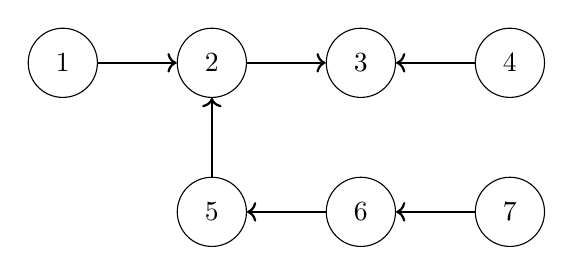
\begin{tikzpicture}
        \node[state](u1){1};
        \node[state, right=of u1](u2){2};
        \node[state, right=of u2](u3){3};
        \node[state, right=of u3](u4){4};
        \node[state, below=of u2](u5){5};
        \node[state, below=of u3](u6){6};
        \node[state, below=of u4](u7){7};
        \draw[->, thick] (u1) -- (u2);
        \draw[->, thick] (u2) -- (u3);
        \draw[->, thick] (u4) -- (u3);
        \draw[->, thick] (u5) -- (u2);
        \draw[->, thick] (u6) -- (u5);
        \draw[->, thick] (u7) -- (u6);
    \end{tikzpicture}
    \caption{Spanning tree of a graph rooted at vertex 3}
    \label{fig:example_spanning_tree}
\end{figure}

Additionally, let us denote the set of all spanning trees of \(G\) as \(T(G)\) and the subset of \(T(G)\) that includes only the spanning trees that are rooted at vertex \(v\) as \(T_v(G)\). The weight of a spanning tree \(t\) can be defined as the product of the weights of the edges it contains: 
\[w(t)=\prod_{e \in t} w(e)\]



\textbf{Theorem: Markov chain tree theorem} \newline
\textit{Let M be an irreducible Markov chain on n states with stationary distribution \(\pi_1, \pi_2, \dots, \pi_n\). Let \(G_M\) be the directed graph associated with \(M\). Then the probability of being at state \(u\) is given by:}

\begin{equation}\label{markov-chain-tree-theorem}
    \pi_i = \frac{\sum_{t \in T_i(G_M)} w(t)}{\sum_{t \in T(G_M)}w(t)}
\end{equation}

Equation \ref{markov-chain-tree-theorem} states that the probability of being at state \(u\) can be found by dividing the sum of the weights of all spanning trees rooted at \(u\) by the sum of the weights of all spanning trees of the graph. Let us ignore the denominator of that fraction for now and focus only on the numerator denoted as \(\tilde{\pi}_i=\sum_{t \in T_i(G_M)} w(t)\)

 

\newpage
\subsubsection{Spanning Trees rooted at \((0,0)\)}

Let us now consider some examples of spanning trees that are rooted at \((0,0)\). For each of the following examples the complete model is shown, then all possible spanning trees rooted at \((0,0)\) along with the weight associated with each spanning tree and finally the value of \(\tilde{\pi}_{(0,0)}\) which is the sum of all the weights of the spanning trees.

\begin{figure}[h]
    \centering
    \documentclass{article}

\usepackage{amsmath}
\usepackage{mathtools}
\usepackage{amsfonts} 
\usepackage{geometry}
\usepackage{graphicx}
\usepackage{soul}
\usepackage{indentfirst}
\usepackage{multicol}
\usepackage{tikz}
\usetikzlibrary{calc, automata, chains, arrows.meta, math}



\title{A game theoretic model of the behavioural gaming that takes place at the EMS - ED interface}
\author{}
\date{}

\begin{document}
\maketitle

\documentclass{article}

\usepackage{amsmath}
\usepackage{mathtools}
\usepackage{amsfonts} 
\usepackage{geometry}
\usepackage{graphicx}
\usepackage{soul}
\usepackage{indentfirst}
\usepackage{multicol}
\usepackage{tikz}
\usetikzlibrary{calc, automata, chains, arrows.meta, math}



\title{A game theoretic model of the behavioural gaming that takes place at the EMS - ED interface}
\author{}
\date{}

\begin{document}
\maketitle

\documentclass{article}

\usepackage{amsmath}
\usepackage{mathtools}
\usepackage{amsfonts} 
\usepackage{geometry}
\usepackage{graphicx}
\usepackage{soul}
\usepackage{indentfirst}
\usepackage{multicol}
\usepackage{tikz}
\usetikzlibrary{calc, automata, chains, arrows.meta, math}



\title{A game theoretic model of the behavioural gaming that takes place at the EMS - ED interface}
\author{}
\date{}

\begin{document}
\maketitle

\input{Abstract/main.tex}
\newpage

% Introduction of the project
\input{Introduction/main.tex}

% Game Theoretic Component
\input{Game_theory_component/main.tex}


\newpage
% Quick representation of the steps of methodology
\input{Methodology/Quick/main.tex}

\newpage
% Proper methodology
\input{Methodology/Proper/main.tex}

% Markov Chains
\input{MarkovChain/main.tex}

\newpage
% Heatmap comparisons
\input{Comparisons/Example_model/main.tex}


\newpage
\input{Miscellaneous/Useful_tikz/main.tex}


% Formulas used
\newpage
\input{Miscellaneous/Formulas/main.tex}

\end{document}

\newpage

% Introduction of the project
\documentclass{article}

\usepackage{amsmath}
\usepackage{mathtools}
\usepackage{amsfonts} 
\usepackage{geometry}
\usepackage{graphicx}
\usepackage{soul}
\usepackage{indentfirst}
\usepackage{multicol}
\usepackage{tikz}
\usetikzlibrary{calc, automata, chains, arrows.meta, math}



\title{A game theoretic model of the behavioural gaming that takes place at the EMS - ED interface}
\author{}
\date{}

\begin{document}
\maketitle

\input{Abstract/main.tex}
\newpage

% Introduction of the project
\input{Introduction/main.tex}

% Game Theoretic Component
\input{Game_theory_component/main.tex}


\newpage
% Quick representation of the steps of methodology
\input{Methodology/Quick/main.tex}

\newpage
% Proper methodology
\input{Methodology/Proper/main.tex}

% Markov Chains
\input{MarkovChain/main.tex}

\newpage
% Heatmap comparisons
\input{Comparisons/Example_model/main.tex}


\newpage
\input{Miscellaneous/Useful_tikz/main.tex}


% Formulas used
\newpage
\input{Miscellaneous/Formulas/main.tex}

\end{document}


% Game Theoretic Component
\documentclass{article}

\usepackage{amsmath}
\usepackage{mathtools}
\usepackage{amsfonts} 
\usepackage{geometry}
\usepackage{graphicx}
\usepackage{soul}
\usepackage{indentfirst}
\usepackage{multicol}
\usepackage{tikz}
\usetikzlibrary{calc, automata, chains, arrows.meta, math}



\title{A game theoretic model of the behavioural gaming that takes place at the EMS - ED interface}
\author{}
\date{}

\begin{document}
\maketitle

\input{Abstract/main.tex}
\newpage

% Introduction of the project
\input{Introduction/main.tex}

% Game Theoretic Component
\input{Game_theory_component/main.tex}


\newpage
% Quick representation of the steps of methodology
\input{Methodology/Quick/main.tex}

\newpage
% Proper methodology
\input{Methodology/Proper/main.tex}

% Markov Chains
\input{MarkovChain/main.tex}

\newpage
% Heatmap comparisons
\input{Comparisons/Example_model/main.tex}


\newpage
\input{Miscellaneous/Useful_tikz/main.tex}


% Formulas used
\newpage
\input{Miscellaneous/Formulas/main.tex}

\end{document}



\newpage
% Quick representation of the steps of methodology
\documentclass{article}

\usepackage{amsmath}
\usepackage{mathtools}
\usepackage{amsfonts} 
\usepackage{geometry}
\usepackage{graphicx}
\usepackage{soul}
\usepackage{indentfirst}
\usepackage{multicol}
\usepackage{tikz}
\usetikzlibrary{calc, automata, chains, arrows.meta, math}



\title{A game theoretic model of the behavioural gaming that takes place at the EMS - ED interface}
\author{}
\date{}

\begin{document}
\maketitle

\input{Abstract/main.tex}
\newpage

% Introduction of the project
\input{Introduction/main.tex}

% Game Theoretic Component
\input{Game_theory_component/main.tex}


\newpage
% Quick representation of the steps of methodology
\input{Methodology/Quick/main.tex}

\newpage
% Proper methodology
\input{Methodology/Proper/main.tex}

% Markov Chains
\input{MarkovChain/main.tex}

\newpage
% Heatmap comparisons
\input{Comparisons/Example_model/main.tex}


\newpage
\input{Miscellaneous/Useful_tikz/main.tex}


% Formulas used
\newpage
\input{Miscellaneous/Formulas/main.tex}

\end{document}


\newpage
% Proper methodology
\documentclass{article}

\usepackage{amsmath}
\usepackage{mathtools}
\usepackage{amsfonts} 
\usepackage{geometry}
\usepackage{graphicx}
\usepackage{soul}
\usepackage{indentfirst}
\usepackage{multicol}
\usepackage{tikz}
\usetikzlibrary{calc, automata, chains, arrows.meta, math}



\title{A game theoretic model of the behavioural gaming that takes place at the EMS - ED interface}
\author{}
\date{}

\begin{document}
\maketitle

\input{Abstract/main.tex}
\newpage

% Introduction of the project
\input{Introduction/main.tex}

% Game Theoretic Component
\input{Game_theory_component/main.tex}


\newpage
% Quick representation of the steps of methodology
\input{Methodology/Quick/main.tex}

\newpage
% Proper methodology
\input{Methodology/Proper/main.tex}

% Markov Chains
\input{MarkovChain/main.tex}

\newpage
% Heatmap comparisons
\input{Comparisons/Example_model/main.tex}


\newpage
\input{Miscellaneous/Useful_tikz/main.tex}


% Formulas used
\newpage
\input{Miscellaneous/Formulas/main.tex}

\end{document}


% Markov Chains
\documentclass{article}

\usepackage{amsmath}
\usepackage{mathtools}
\usepackage{amsfonts} 
\usepackage{geometry}
\usepackage{graphicx}
\usepackage{soul}
\usepackage{indentfirst}
\usepackage{multicol}
\usepackage{tikz}
\usetikzlibrary{calc, automata, chains, arrows.meta, math}



\title{A game theoretic model of the behavioural gaming that takes place at the EMS - ED interface}
\author{}
\date{}

\begin{document}
\maketitle

\input{Abstract/main.tex}
\newpage

% Introduction of the project
\input{Introduction/main.tex}

% Game Theoretic Component
\input{Game_theory_component/main.tex}


\newpage
% Quick representation of the steps of methodology
\input{Methodology/Quick/main.tex}

\newpage
% Proper methodology
\input{Methodology/Proper/main.tex}

% Markov Chains
\input{MarkovChain/main.tex}

\newpage
% Heatmap comparisons
\input{Comparisons/Example_model/main.tex}


\newpage
\input{Miscellaneous/Useful_tikz/main.tex}


% Formulas used
\newpage
\input{Miscellaneous/Formulas/main.tex}

\end{document}


\newpage
% Heatmap comparisons
\documentclass{article}

\usepackage{amsmath}
\usepackage{mathtools}
\usepackage{amsfonts} 
\usepackage{geometry}
\usepackage{graphicx}
\usepackage{soul}
\usepackage{indentfirst}
\usepackage{multicol}
\usepackage{tikz}
\usetikzlibrary{calc, automata, chains, arrows.meta, math}



\title{A game theoretic model of the behavioural gaming that takes place at the EMS - ED interface}
\author{}
\date{}

\begin{document}
\maketitle

\input{Abstract/main.tex}
\newpage

% Introduction of the project
\input{Introduction/main.tex}

% Game Theoretic Component
\input{Game_theory_component/main.tex}


\newpage
% Quick representation of the steps of methodology
\input{Methodology/Quick/main.tex}

\newpage
% Proper methodology
\input{Methodology/Proper/main.tex}

% Markov Chains
\input{MarkovChain/main.tex}

\newpage
% Heatmap comparisons
\input{Comparisons/Example_model/main.tex}


\newpage
\input{Miscellaneous/Useful_tikz/main.tex}


% Formulas used
\newpage
\input{Miscellaneous/Formulas/main.tex}

\end{document}



\newpage
\documentclass{article}

\usepackage{amsmath}
\usepackage{mathtools}
\usepackage{amsfonts} 
\usepackage{geometry}
\usepackage{graphicx}
\usepackage{soul}
\usepackage{indentfirst}
\usepackage{multicol}
\usepackage{tikz}
\usetikzlibrary{calc, automata, chains, arrows.meta, math}



\title{A game theoretic model of the behavioural gaming that takes place at the EMS - ED interface}
\author{}
\date{}

\begin{document}
\maketitle

\input{Abstract/main.tex}
\newpage

% Introduction of the project
\input{Introduction/main.tex}

% Game Theoretic Component
\input{Game_theory_component/main.tex}


\newpage
% Quick representation of the steps of methodology
\input{Methodology/Quick/main.tex}

\newpage
% Proper methodology
\input{Methodology/Proper/main.tex}

% Markov Chains
\input{MarkovChain/main.tex}

\newpage
% Heatmap comparisons
\input{Comparisons/Example_model/main.tex}


\newpage
\input{Miscellaneous/Useful_tikz/main.tex}


% Formulas used
\newpage
\input{Miscellaneous/Formulas/main.tex}

\end{document}



% Formulas used
\newpage
\documentclass{article}

\usepackage{amsmath}
\usepackage{mathtools}
\usepackage{amsfonts} 
\usepackage{geometry}
\usepackage{graphicx}
\usepackage{soul}
\usepackage{indentfirst}
\usepackage{multicol}
\usepackage{tikz}
\usetikzlibrary{calc, automata, chains, arrows.meta, math}



\title{A game theoretic model of the behavioural gaming that takes place at the EMS - ED interface}
\author{}
\date{}

\begin{document}
\maketitle

\input{Abstract/main.tex}
\newpage

% Introduction of the project
\input{Introduction/main.tex}

% Game Theoretic Component
\input{Game_theory_component/main.tex}


\newpage
% Quick representation of the steps of methodology
\input{Methodology/Quick/main.tex}

\newpage
% Proper methodology
\input{Methodology/Proper/main.tex}

% Markov Chains
\input{MarkovChain/main.tex}

\newpage
% Heatmap comparisons
\input{Comparisons/Example_model/main.tex}


\newpage
\input{Miscellaneous/Useful_tikz/main.tex}


% Formulas used
\newpage
\input{Miscellaneous/Formulas/main.tex}

\end{document}


\end{document}

\newpage

% Introduction of the project
\documentclass{article}

\usepackage{amsmath}
\usepackage{mathtools}
\usepackage{amsfonts} 
\usepackage{geometry}
\usepackage{graphicx}
\usepackage{soul}
\usepackage{indentfirst}
\usepackage{multicol}
\usepackage{tikz}
\usetikzlibrary{calc, automata, chains, arrows.meta, math}



\title{A game theoretic model of the behavioural gaming that takes place at the EMS - ED interface}
\author{}
\date{}

\begin{document}
\maketitle

\documentclass{article}

\usepackage{amsmath}
\usepackage{mathtools}
\usepackage{amsfonts} 
\usepackage{geometry}
\usepackage{graphicx}
\usepackage{soul}
\usepackage{indentfirst}
\usepackage{multicol}
\usepackage{tikz}
\usetikzlibrary{calc, automata, chains, arrows.meta, math}



\title{A game theoretic model of the behavioural gaming that takes place at the EMS - ED interface}
\author{}
\date{}

\begin{document}
\maketitle

\input{Abstract/main.tex}
\newpage

% Introduction of the project
\input{Introduction/main.tex}

% Game Theoretic Component
\input{Game_theory_component/main.tex}


\newpage
% Quick representation of the steps of methodology
\input{Methodology/Quick/main.tex}

\newpage
% Proper methodology
\input{Methodology/Proper/main.tex}

% Markov Chains
\input{MarkovChain/main.tex}

\newpage
% Heatmap comparisons
\input{Comparisons/Example_model/main.tex}


\newpage
\input{Miscellaneous/Useful_tikz/main.tex}


% Formulas used
\newpage
\input{Miscellaneous/Formulas/main.tex}

\end{document}

\newpage

% Introduction of the project
\documentclass{article}

\usepackage{amsmath}
\usepackage{mathtools}
\usepackage{amsfonts} 
\usepackage{geometry}
\usepackage{graphicx}
\usepackage{soul}
\usepackage{indentfirst}
\usepackage{multicol}
\usepackage{tikz}
\usetikzlibrary{calc, automata, chains, arrows.meta, math}



\title{A game theoretic model of the behavioural gaming that takes place at the EMS - ED interface}
\author{}
\date{}

\begin{document}
\maketitle

\input{Abstract/main.tex}
\newpage

% Introduction of the project
\input{Introduction/main.tex}

% Game Theoretic Component
\input{Game_theory_component/main.tex}


\newpage
% Quick representation of the steps of methodology
\input{Methodology/Quick/main.tex}

\newpage
% Proper methodology
\input{Methodology/Proper/main.tex}

% Markov Chains
\input{MarkovChain/main.tex}

\newpage
% Heatmap comparisons
\input{Comparisons/Example_model/main.tex}


\newpage
\input{Miscellaneous/Useful_tikz/main.tex}


% Formulas used
\newpage
\input{Miscellaneous/Formulas/main.tex}

\end{document}


% Game Theoretic Component
\documentclass{article}

\usepackage{amsmath}
\usepackage{mathtools}
\usepackage{amsfonts} 
\usepackage{geometry}
\usepackage{graphicx}
\usepackage{soul}
\usepackage{indentfirst}
\usepackage{multicol}
\usepackage{tikz}
\usetikzlibrary{calc, automata, chains, arrows.meta, math}



\title{A game theoretic model of the behavioural gaming that takes place at the EMS - ED interface}
\author{}
\date{}

\begin{document}
\maketitle

\input{Abstract/main.tex}
\newpage

% Introduction of the project
\input{Introduction/main.tex}

% Game Theoretic Component
\input{Game_theory_component/main.tex}


\newpage
% Quick representation of the steps of methodology
\input{Methodology/Quick/main.tex}

\newpage
% Proper methodology
\input{Methodology/Proper/main.tex}

% Markov Chains
\input{MarkovChain/main.tex}

\newpage
% Heatmap comparisons
\input{Comparisons/Example_model/main.tex}


\newpage
\input{Miscellaneous/Useful_tikz/main.tex}


% Formulas used
\newpage
\input{Miscellaneous/Formulas/main.tex}

\end{document}



\newpage
% Quick representation of the steps of methodology
\documentclass{article}

\usepackage{amsmath}
\usepackage{mathtools}
\usepackage{amsfonts} 
\usepackage{geometry}
\usepackage{graphicx}
\usepackage{soul}
\usepackage{indentfirst}
\usepackage{multicol}
\usepackage{tikz}
\usetikzlibrary{calc, automata, chains, arrows.meta, math}



\title{A game theoretic model of the behavioural gaming that takes place at the EMS - ED interface}
\author{}
\date{}

\begin{document}
\maketitle

\input{Abstract/main.tex}
\newpage

% Introduction of the project
\input{Introduction/main.tex}

% Game Theoretic Component
\input{Game_theory_component/main.tex}


\newpage
% Quick representation of the steps of methodology
\input{Methodology/Quick/main.tex}

\newpage
% Proper methodology
\input{Methodology/Proper/main.tex}

% Markov Chains
\input{MarkovChain/main.tex}

\newpage
% Heatmap comparisons
\input{Comparisons/Example_model/main.tex}


\newpage
\input{Miscellaneous/Useful_tikz/main.tex}


% Formulas used
\newpage
\input{Miscellaneous/Formulas/main.tex}

\end{document}


\newpage
% Proper methodology
\documentclass{article}

\usepackage{amsmath}
\usepackage{mathtools}
\usepackage{amsfonts} 
\usepackage{geometry}
\usepackage{graphicx}
\usepackage{soul}
\usepackage{indentfirst}
\usepackage{multicol}
\usepackage{tikz}
\usetikzlibrary{calc, automata, chains, arrows.meta, math}



\title{A game theoretic model of the behavioural gaming that takes place at the EMS - ED interface}
\author{}
\date{}

\begin{document}
\maketitle

\input{Abstract/main.tex}
\newpage

% Introduction of the project
\input{Introduction/main.tex}

% Game Theoretic Component
\input{Game_theory_component/main.tex}


\newpage
% Quick representation of the steps of methodology
\input{Methodology/Quick/main.tex}

\newpage
% Proper methodology
\input{Methodology/Proper/main.tex}

% Markov Chains
\input{MarkovChain/main.tex}

\newpage
% Heatmap comparisons
\input{Comparisons/Example_model/main.tex}


\newpage
\input{Miscellaneous/Useful_tikz/main.tex}


% Formulas used
\newpage
\input{Miscellaneous/Formulas/main.tex}

\end{document}


% Markov Chains
\documentclass{article}

\usepackage{amsmath}
\usepackage{mathtools}
\usepackage{amsfonts} 
\usepackage{geometry}
\usepackage{graphicx}
\usepackage{soul}
\usepackage{indentfirst}
\usepackage{multicol}
\usepackage{tikz}
\usetikzlibrary{calc, automata, chains, arrows.meta, math}



\title{A game theoretic model of the behavioural gaming that takes place at the EMS - ED interface}
\author{}
\date{}

\begin{document}
\maketitle

\input{Abstract/main.tex}
\newpage

% Introduction of the project
\input{Introduction/main.tex}

% Game Theoretic Component
\input{Game_theory_component/main.tex}


\newpage
% Quick representation of the steps of methodology
\input{Methodology/Quick/main.tex}

\newpage
% Proper methodology
\input{Methodology/Proper/main.tex}

% Markov Chains
\input{MarkovChain/main.tex}

\newpage
% Heatmap comparisons
\input{Comparisons/Example_model/main.tex}


\newpage
\input{Miscellaneous/Useful_tikz/main.tex}


% Formulas used
\newpage
\input{Miscellaneous/Formulas/main.tex}

\end{document}


\newpage
% Heatmap comparisons
\documentclass{article}

\usepackage{amsmath}
\usepackage{mathtools}
\usepackage{amsfonts} 
\usepackage{geometry}
\usepackage{graphicx}
\usepackage{soul}
\usepackage{indentfirst}
\usepackage{multicol}
\usepackage{tikz}
\usetikzlibrary{calc, automata, chains, arrows.meta, math}



\title{A game theoretic model of the behavioural gaming that takes place at the EMS - ED interface}
\author{}
\date{}

\begin{document}
\maketitle

\input{Abstract/main.tex}
\newpage

% Introduction of the project
\input{Introduction/main.tex}

% Game Theoretic Component
\input{Game_theory_component/main.tex}


\newpage
% Quick representation of the steps of methodology
\input{Methodology/Quick/main.tex}

\newpage
% Proper methodology
\input{Methodology/Proper/main.tex}

% Markov Chains
\input{MarkovChain/main.tex}

\newpage
% Heatmap comparisons
\input{Comparisons/Example_model/main.tex}


\newpage
\input{Miscellaneous/Useful_tikz/main.tex}


% Formulas used
\newpage
\input{Miscellaneous/Formulas/main.tex}

\end{document}



\newpage
\documentclass{article}

\usepackage{amsmath}
\usepackage{mathtools}
\usepackage{amsfonts} 
\usepackage{geometry}
\usepackage{graphicx}
\usepackage{soul}
\usepackage{indentfirst}
\usepackage{multicol}
\usepackage{tikz}
\usetikzlibrary{calc, automata, chains, arrows.meta, math}



\title{A game theoretic model of the behavioural gaming that takes place at the EMS - ED interface}
\author{}
\date{}

\begin{document}
\maketitle

\input{Abstract/main.tex}
\newpage

% Introduction of the project
\input{Introduction/main.tex}

% Game Theoretic Component
\input{Game_theory_component/main.tex}


\newpage
% Quick representation of the steps of methodology
\input{Methodology/Quick/main.tex}

\newpage
% Proper methodology
\input{Methodology/Proper/main.tex}

% Markov Chains
\input{MarkovChain/main.tex}

\newpage
% Heatmap comparisons
\input{Comparisons/Example_model/main.tex}


\newpage
\input{Miscellaneous/Useful_tikz/main.tex}


% Formulas used
\newpage
\input{Miscellaneous/Formulas/main.tex}

\end{document}



% Formulas used
\newpage
\documentclass{article}

\usepackage{amsmath}
\usepackage{mathtools}
\usepackage{amsfonts} 
\usepackage{geometry}
\usepackage{graphicx}
\usepackage{soul}
\usepackage{indentfirst}
\usepackage{multicol}
\usepackage{tikz}
\usetikzlibrary{calc, automata, chains, arrows.meta, math}



\title{A game theoretic model of the behavioural gaming that takes place at the EMS - ED interface}
\author{}
\date{}

\begin{document}
\maketitle

\input{Abstract/main.tex}
\newpage

% Introduction of the project
\input{Introduction/main.tex}

% Game Theoretic Component
\input{Game_theory_component/main.tex}


\newpage
% Quick representation of the steps of methodology
\input{Methodology/Quick/main.tex}

\newpage
% Proper methodology
\input{Methodology/Proper/main.tex}

% Markov Chains
\input{MarkovChain/main.tex}

\newpage
% Heatmap comparisons
\input{Comparisons/Example_model/main.tex}


\newpage
\input{Miscellaneous/Useful_tikz/main.tex}


% Formulas used
\newpage
\input{Miscellaneous/Formulas/main.tex}

\end{document}


\end{document}


% Game Theoretic Component
\documentclass{article}

\usepackage{amsmath}
\usepackage{mathtools}
\usepackage{amsfonts} 
\usepackage{geometry}
\usepackage{graphicx}
\usepackage{soul}
\usepackage{indentfirst}
\usepackage{multicol}
\usepackage{tikz}
\usetikzlibrary{calc, automata, chains, arrows.meta, math}



\title{A game theoretic model of the behavioural gaming that takes place at the EMS - ED interface}
\author{}
\date{}

\begin{document}
\maketitle

\documentclass{article}

\usepackage{amsmath}
\usepackage{mathtools}
\usepackage{amsfonts} 
\usepackage{geometry}
\usepackage{graphicx}
\usepackage{soul}
\usepackage{indentfirst}
\usepackage{multicol}
\usepackage{tikz}
\usetikzlibrary{calc, automata, chains, arrows.meta, math}



\title{A game theoretic model of the behavioural gaming that takes place at the EMS - ED interface}
\author{}
\date{}

\begin{document}
\maketitle

\input{Abstract/main.tex}
\newpage

% Introduction of the project
\input{Introduction/main.tex}

% Game Theoretic Component
\input{Game_theory_component/main.tex}


\newpage
% Quick representation of the steps of methodology
\input{Methodology/Quick/main.tex}

\newpage
% Proper methodology
\input{Methodology/Proper/main.tex}

% Markov Chains
\input{MarkovChain/main.tex}

\newpage
% Heatmap comparisons
\input{Comparisons/Example_model/main.tex}


\newpage
\input{Miscellaneous/Useful_tikz/main.tex}


% Formulas used
\newpage
\input{Miscellaneous/Formulas/main.tex}

\end{document}

\newpage

% Introduction of the project
\documentclass{article}

\usepackage{amsmath}
\usepackage{mathtools}
\usepackage{amsfonts} 
\usepackage{geometry}
\usepackage{graphicx}
\usepackage{soul}
\usepackage{indentfirst}
\usepackage{multicol}
\usepackage{tikz}
\usetikzlibrary{calc, automata, chains, arrows.meta, math}



\title{A game theoretic model of the behavioural gaming that takes place at the EMS - ED interface}
\author{}
\date{}

\begin{document}
\maketitle

\input{Abstract/main.tex}
\newpage

% Introduction of the project
\input{Introduction/main.tex}

% Game Theoretic Component
\input{Game_theory_component/main.tex}


\newpage
% Quick representation of the steps of methodology
\input{Methodology/Quick/main.tex}

\newpage
% Proper methodology
\input{Methodology/Proper/main.tex}

% Markov Chains
\input{MarkovChain/main.tex}

\newpage
% Heatmap comparisons
\input{Comparisons/Example_model/main.tex}


\newpage
\input{Miscellaneous/Useful_tikz/main.tex}


% Formulas used
\newpage
\input{Miscellaneous/Formulas/main.tex}

\end{document}


% Game Theoretic Component
\documentclass{article}

\usepackage{amsmath}
\usepackage{mathtools}
\usepackage{amsfonts} 
\usepackage{geometry}
\usepackage{graphicx}
\usepackage{soul}
\usepackage{indentfirst}
\usepackage{multicol}
\usepackage{tikz}
\usetikzlibrary{calc, automata, chains, arrows.meta, math}



\title{A game theoretic model of the behavioural gaming that takes place at the EMS - ED interface}
\author{}
\date{}

\begin{document}
\maketitle

\input{Abstract/main.tex}
\newpage

% Introduction of the project
\input{Introduction/main.tex}

% Game Theoretic Component
\input{Game_theory_component/main.tex}


\newpage
% Quick representation of the steps of methodology
\input{Methodology/Quick/main.tex}

\newpage
% Proper methodology
\input{Methodology/Proper/main.tex}

% Markov Chains
\input{MarkovChain/main.tex}

\newpage
% Heatmap comparisons
\input{Comparisons/Example_model/main.tex}


\newpage
\input{Miscellaneous/Useful_tikz/main.tex}


% Formulas used
\newpage
\input{Miscellaneous/Formulas/main.tex}

\end{document}



\newpage
% Quick representation of the steps of methodology
\documentclass{article}

\usepackage{amsmath}
\usepackage{mathtools}
\usepackage{amsfonts} 
\usepackage{geometry}
\usepackage{graphicx}
\usepackage{soul}
\usepackage{indentfirst}
\usepackage{multicol}
\usepackage{tikz}
\usetikzlibrary{calc, automata, chains, arrows.meta, math}



\title{A game theoretic model of the behavioural gaming that takes place at the EMS - ED interface}
\author{}
\date{}

\begin{document}
\maketitle

\input{Abstract/main.tex}
\newpage

% Introduction of the project
\input{Introduction/main.tex}

% Game Theoretic Component
\input{Game_theory_component/main.tex}


\newpage
% Quick representation of the steps of methodology
\input{Methodology/Quick/main.tex}

\newpage
% Proper methodology
\input{Methodology/Proper/main.tex}

% Markov Chains
\input{MarkovChain/main.tex}

\newpage
% Heatmap comparisons
\input{Comparisons/Example_model/main.tex}


\newpage
\input{Miscellaneous/Useful_tikz/main.tex}


% Formulas used
\newpage
\input{Miscellaneous/Formulas/main.tex}

\end{document}


\newpage
% Proper methodology
\documentclass{article}

\usepackage{amsmath}
\usepackage{mathtools}
\usepackage{amsfonts} 
\usepackage{geometry}
\usepackage{graphicx}
\usepackage{soul}
\usepackage{indentfirst}
\usepackage{multicol}
\usepackage{tikz}
\usetikzlibrary{calc, automata, chains, arrows.meta, math}



\title{A game theoretic model of the behavioural gaming that takes place at the EMS - ED interface}
\author{}
\date{}

\begin{document}
\maketitle

\input{Abstract/main.tex}
\newpage

% Introduction of the project
\input{Introduction/main.tex}

% Game Theoretic Component
\input{Game_theory_component/main.tex}


\newpage
% Quick representation of the steps of methodology
\input{Methodology/Quick/main.tex}

\newpage
% Proper methodology
\input{Methodology/Proper/main.tex}

% Markov Chains
\input{MarkovChain/main.tex}

\newpage
% Heatmap comparisons
\input{Comparisons/Example_model/main.tex}


\newpage
\input{Miscellaneous/Useful_tikz/main.tex}


% Formulas used
\newpage
\input{Miscellaneous/Formulas/main.tex}

\end{document}


% Markov Chains
\documentclass{article}

\usepackage{amsmath}
\usepackage{mathtools}
\usepackage{amsfonts} 
\usepackage{geometry}
\usepackage{graphicx}
\usepackage{soul}
\usepackage{indentfirst}
\usepackage{multicol}
\usepackage{tikz}
\usetikzlibrary{calc, automata, chains, arrows.meta, math}



\title{A game theoretic model of the behavioural gaming that takes place at the EMS - ED interface}
\author{}
\date{}

\begin{document}
\maketitle

\input{Abstract/main.tex}
\newpage

% Introduction of the project
\input{Introduction/main.tex}

% Game Theoretic Component
\input{Game_theory_component/main.tex}


\newpage
% Quick representation of the steps of methodology
\input{Methodology/Quick/main.tex}

\newpage
% Proper methodology
\input{Methodology/Proper/main.tex}

% Markov Chains
\input{MarkovChain/main.tex}

\newpage
% Heatmap comparisons
\input{Comparisons/Example_model/main.tex}


\newpage
\input{Miscellaneous/Useful_tikz/main.tex}


% Formulas used
\newpage
\input{Miscellaneous/Formulas/main.tex}

\end{document}


\newpage
% Heatmap comparisons
\documentclass{article}

\usepackage{amsmath}
\usepackage{mathtools}
\usepackage{amsfonts} 
\usepackage{geometry}
\usepackage{graphicx}
\usepackage{soul}
\usepackage{indentfirst}
\usepackage{multicol}
\usepackage{tikz}
\usetikzlibrary{calc, automata, chains, arrows.meta, math}



\title{A game theoretic model of the behavioural gaming that takes place at the EMS - ED interface}
\author{}
\date{}

\begin{document}
\maketitle

\input{Abstract/main.tex}
\newpage

% Introduction of the project
\input{Introduction/main.tex}

% Game Theoretic Component
\input{Game_theory_component/main.tex}


\newpage
% Quick representation of the steps of methodology
\input{Methodology/Quick/main.tex}

\newpage
% Proper methodology
\input{Methodology/Proper/main.tex}

% Markov Chains
\input{MarkovChain/main.tex}

\newpage
% Heatmap comparisons
\input{Comparisons/Example_model/main.tex}


\newpage
\input{Miscellaneous/Useful_tikz/main.tex}


% Formulas used
\newpage
\input{Miscellaneous/Formulas/main.tex}

\end{document}



\newpage
\documentclass{article}

\usepackage{amsmath}
\usepackage{mathtools}
\usepackage{amsfonts} 
\usepackage{geometry}
\usepackage{graphicx}
\usepackage{soul}
\usepackage{indentfirst}
\usepackage{multicol}
\usepackage{tikz}
\usetikzlibrary{calc, automata, chains, arrows.meta, math}



\title{A game theoretic model of the behavioural gaming that takes place at the EMS - ED interface}
\author{}
\date{}

\begin{document}
\maketitle

\input{Abstract/main.tex}
\newpage

% Introduction of the project
\input{Introduction/main.tex}

% Game Theoretic Component
\input{Game_theory_component/main.tex}


\newpage
% Quick representation of the steps of methodology
\input{Methodology/Quick/main.tex}

\newpage
% Proper methodology
\input{Methodology/Proper/main.tex}

% Markov Chains
\input{MarkovChain/main.tex}

\newpage
% Heatmap comparisons
\input{Comparisons/Example_model/main.tex}


\newpage
\input{Miscellaneous/Useful_tikz/main.tex}


% Formulas used
\newpage
\input{Miscellaneous/Formulas/main.tex}

\end{document}



% Formulas used
\newpage
\documentclass{article}

\usepackage{amsmath}
\usepackage{mathtools}
\usepackage{amsfonts} 
\usepackage{geometry}
\usepackage{graphicx}
\usepackage{soul}
\usepackage{indentfirst}
\usepackage{multicol}
\usepackage{tikz}
\usetikzlibrary{calc, automata, chains, arrows.meta, math}



\title{A game theoretic model of the behavioural gaming that takes place at the EMS - ED interface}
\author{}
\date{}

\begin{document}
\maketitle

\input{Abstract/main.tex}
\newpage

% Introduction of the project
\input{Introduction/main.tex}

% Game Theoretic Component
\input{Game_theory_component/main.tex}


\newpage
% Quick representation of the steps of methodology
\input{Methodology/Quick/main.tex}

\newpage
% Proper methodology
\input{Methodology/Proper/main.tex}

% Markov Chains
\input{MarkovChain/main.tex}

\newpage
% Heatmap comparisons
\input{Comparisons/Example_model/main.tex}


\newpage
\input{Miscellaneous/Useful_tikz/main.tex}


% Formulas used
\newpage
\input{Miscellaneous/Formulas/main.tex}

\end{document}


\end{document}



\newpage
% Quick representation of the steps of methodology
\documentclass{article}

\usepackage{amsmath}
\usepackage{mathtools}
\usepackage{amsfonts} 
\usepackage{geometry}
\usepackage{graphicx}
\usepackage{soul}
\usepackage{indentfirst}
\usepackage{multicol}
\usepackage{tikz}
\usetikzlibrary{calc, automata, chains, arrows.meta, math}



\title{A game theoretic model of the behavioural gaming that takes place at the EMS - ED interface}
\author{}
\date{}

\begin{document}
\maketitle

\documentclass{article}

\usepackage{amsmath}
\usepackage{mathtools}
\usepackage{amsfonts} 
\usepackage{geometry}
\usepackage{graphicx}
\usepackage{soul}
\usepackage{indentfirst}
\usepackage{multicol}
\usepackage{tikz}
\usetikzlibrary{calc, automata, chains, arrows.meta, math}



\title{A game theoretic model of the behavioural gaming that takes place at the EMS - ED interface}
\author{}
\date{}

\begin{document}
\maketitle

\input{Abstract/main.tex}
\newpage

% Introduction of the project
\input{Introduction/main.tex}

% Game Theoretic Component
\input{Game_theory_component/main.tex}


\newpage
% Quick representation of the steps of methodology
\input{Methodology/Quick/main.tex}

\newpage
% Proper methodology
\input{Methodology/Proper/main.tex}

% Markov Chains
\input{MarkovChain/main.tex}

\newpage
% Heatmap comparisons
\input{Comparisons/Example_model/main.tex}


\newpage
\input{Miscellaneous/Useful_tikz/main.tex}


% Formulas used
\newpage
\input{Miscellaneous/Formulas/main.tex}

\end{document}

\newpage

% Introduction of the project
\documentclass{article}

\usepackage{amsmath}
\usepackage{mathtools}
\usepackage{amsfonts} 
\usepackage{geometry}
\usepackage{graphicx}
\usepackage{soul}
\usepackage{indentfirst}
\usepackage{multicol}
\usepackage{tikz}
\usetikzlibrary{calc, automata, chains, arrows.meta, math}



\title{A game theoretic model of the behavioural gaming that takes place at the EMS - ED interface}
\author{}
\date{}

\begin{document}
\maketitle

\input{Abstract/main.tex}
\newpage

% Introduction of the project
\input{Introduction/main.tex}

% Game Theoretic Component
\input{Game_theory_component/main.tex}


\newpage
% Quick representation of the steps of methodology
\input{Methodology/Quick/main.tex}

\newpage
% Proper methodology
\input{Methodology/Proper/main.tex}

% Markov Chains
\input{MarkovChain/main.tex}

\newpage
% Heatmap comparisons
\input{Comparisons/Example_model/main.tex}


\newpage
\input{Miscellaneous/Useful_tikz/main.tex}


% Formulas used
\newpage
\input{Miscellaneous/Formulas/main.tex}

\end{document}


% Game Theoretic Component
\documentclass{article}

\usepackage{amsmath}
\usepackage{mathtools}
\usepackage{amsfonts} 
\usepackage{geometry}
\usepackage{graphicx}
\usepackage{soul}
\usepackage{indentfirst}
\usepackage{multicol}
\usepackage{tikz}
\usetikzlibrary{calc, automata, chains, arrows.meta, math}



\title{A game theoretic model of the behavioural gaming that takes place at the EMS - ED interface}
\author{}
\date{}

\begin{document}
\maketitle

\input{Abstract/main.tex}
\newpage

% Introduction of the project
\input{Introduction/main.tex}

% Game Theoretic Component
\input{Game_theory_component/main.tex}


\newpage
% Quick representation of the steps of methodology
\input{Methodology/Quick/main.tex}

\newpage
% Proper methodology
\input{Methodology/Proper/main.tex}

% Markov Chains
\input{MarkovChain/main.tex}

\newpage
% Heatmap comparisons
\input{Comparisons/Example_model/main.tex}


\newpage
\input{Miscellaneous/Useful_tikz/main.tex}


% Formulas used
\newpage
\input{Miscellaneous/Formulas/main.tex}

\end{document}



\newpage
% Quick representation of the steps of methodology
\documentclass{article}

\usepackage{amsmath}
\usepackage{mathtools}
\usepackage{amsfonts} 
\usepackage{geometry}
\usepackage{graphicx}
\usepackage{soul}
\usepackage{indentfirst}
\usepackage{multicol}
\usepackage{tikz}
\usetikzlibrary{calc, automata, chains, arrows.meta, math}



\title{A game theoretic model of the behavioural gaming that takes place at the EMS - ED interface}
\author{}
\date{}

\begin{document}
\maketitle

\input{Abstract/main.tex}
\newpage

% Introduction of the project
\input{Introduction/main.tex}

% Game Theoretic Component
\input{Game_theory_component/main.tex}


\newpage
% Quick representation of the steps of methodology
\input{Methodology/Quick/main.tex}

\newpage
% Proper methodology
\input{Methodology/Proper/main.tex}

% Markov Chains
\input{MarkovChain/main.tex}

\newpage
% Heatmap comparisons
\input{Comparisons/Example_model/main.tex}


\newpage
\input{Miscellaneous/Useful_tikz/main.tex}


% Formulas used
\newpage
\input{Miscellaneous/Formulas/main.tex}

\end{document}


\newpage
% Proper methodology
\documentclass{article}

\usepackage{amsmath}
\usepackage{mathtools}
\usepackage{amsfonts} 
\usepackage{geometry}
\usepackage{graphicx}
\usepackage{soul}
\usepackage{indentfirst}
\usepackage{multicol}
\usepackage{tikz}
\usetikzlibrary{calc, automata, chains, arrows.meta, math}



\title{A game theoretic model of the behavioural gaming that takes place at the EMS - ED interface}
\author{}
\date{}

\begin{document}
\maketitle

\input{Abstract/main.tex}
\newpage

% Introduction of the project
\input{Introduction/main.tex}

% Game Theoretic Component
\input{Game_theory_component/main.tex}


\newpage
% Quick representation of the steps of methodology
\input{Methodology/Quick/main.tex}

\newpage
% Proper methodology
\input{Methodology/Proper/main.tex}

% Markov Chains
\input{MarkovChain/main.tex}

\newpage
% Heatmap comparisons
\input{Comparisons/Example_model/main.tex}


\newpage
\input{Miscellaneous/Useful_tikz/main.tex}


% Formulas used
\newpage
\input{Miscellaneous/Formulas/main.tex}

\end{document}


% Markov Chains
\documentclass{article}

\usepackage{amsmath}
\usepackage{mathtools}
\usepackage{amsfonts} 
\usepackage{geometry}
\usepackage{graphicx}
\usepackage{soul}
\usepackage{indentfirst}
\usepackage{multicol}
\usepackage{tikz}
\usetikzlibrary{calc, automata, chains, arrows.meta, math}



\title{A game theoretic model of the behavioural gaming that takes place at the EMS - ED interface}
\author{}
\date{}

\begin{document}
\maketitle

\input{Abstract/main.tex}
\newpage

% Introduction of the project
\input{Introduction/main.tex}

% Game Theoretic Component
\input{Game_theory_component/main.tex}


\newpage
% Quick representation of the steps of methodology
\input{Methodology/Quick/main.tex}

\newpage
% Proper methodology
\input{Methodology/Proper/main.tex}

% Markov Chains
\input{MarkovChain/main.tex}

\newpage
% Heatmap comparisons
\input{Comparisons/Example_model/main.tex}


\newpage
\input{Miscellaneous/Useful_tikz/main.tex}


% Formulas used
\newpage
\input{Miscellaneous/Formulas/main.tex}

\end{document}


\newpage
% Heatmap comparisons
\documentclass{article}

\usepackage{amsmath}
\usepackage{mathtools}
\usepackage{amsfonts} 
\usepackage{geometry}
\usepackage{graphicx}
\usepackage{soul}
\usepackage{indentfirst}
\usepackage{multicol}
\usepackage{tikz}
\usetikzlibrary{calc, automata, chains, arrows.meta, math}



\title{A game theoretic model of the behavioural gaming that takes place at the EMS - ED interface}
\author{}
\date{}

\begin{document}
\maketitle

\input{Abstract/main.tex}
\newpage

% Introduction of the project
\input{Introduction/main.tex}

% Game Theoretic Component
\input{Game_theory_component/main.tex}


\newpage
% Quick representation of the steps of methodology
\input{Methodology/Quick/main.tex}

\newpage
% Proper methodology
\input{Methodology/Proper/main.tex}

% Markov Chains
\input{MarkovChain/main.tex}

\newpage
% Heatmap comparisons
\input{Comparisons/Example_model/main.tex}


\newpage
\input{Miscellaneous/Useful_tikz/main.tex}


% Formulas used
\newpage
\input{Miscellaneous/Formulas/main.tex}

\end{document}



\newpage
\documentclass{article}

\usepackage{amsmath}
\usepackage{mathtools}
\usepackage{amsfonts} 
\usepackage{geometry}
\usepackage{graphicx}
\usepackage{soul}
\usepackage{indentfirst}
\usepackage{multicol}
\usepackage{tikz}
\usetikzlibrary{calc, automata, chains, arrows.meta, math}



\title{A game theoretic model of the behavioural gaming that takes place at the EMS - ED interface}
\author{}
\date{}

\begin{document}
\maketitle

\input{Abstract/main.tex}
\newpage

% Introduction of the project
\input{Introduction/main.tex}

% Game Theoretic Component
\input{Game_theory_component/main.tex}


\newpage
% Quick representation of the steps of methodology
\input{Methodology/Quick/main.tex}

\newpage
% Proper methodology
\input{Methodology/Proper/main.tex}

% Markov Chains
\input{MarkovChain/main.tex}

\newpage
% Heatmap comparisons
\input{Comparisons/Example_model/main.tex}


\newpage
\input{Miscellaneous/Useful_tikz/main.tex}


% Formulas used
\newpage
\input{Miscellaneous/Formulas/main.tex}

\end{document}



% Formulas used
\newpage
\documentclass{article}

\usepackage{amsmath}
\usepackage{mathtools}
\usepackage{amsfonts} 
\usepackage{geometry}
\usepackage{graphicx}
\usepackage{soul}
\usepackage{indentfirst}
\usepackage{multicol}
\usepackage{tikz}
\usetikzlibrary{calc, automata, chains, arrows.meta, math}



\title{A game theoretic model of the behavioural gaming that takes place at the EMS - ED interface}
\author{}
\date{}

\begin{document}
\maketitle

\input{Abstract/main.tex}
\newpage

% Introduction of the project
\input{Introduction/main.tex}

% Game Theoretic Component
\input{Game_theory_component/main.tex}


\newpage
% Quick representation of the steps of methodology
\input{Methodology/Quick/main.tex}

\newpage
% Proper methodology
\input{Methodology/Proper/main.tex}

% Markov Chains
\input{MarkovChain/main.tex}

\newpage
% Heatmap comparisons
\input{Comparisons/Example_model/main.tex}


\newpage
\input{Miscellaneous/Useful_tikz/main.tex}


% Formulas used
\newpage
\input{Miscellaneous/Formulas/main.tex}

\end{document}


\end{document}


\newpage
% Proper methodology
\documentclass{article}

\usepackage{amsmath}
\usepackage{mathtools}
\usepackage{amsfonts} 
\usepackage{geometry}
\usepackage{graphicx}
\usepackage{soul}
\usepackage{indentfirst}
\usepackage{multicol}
\usepackage{tikz}
\usetikzlibrary{calc, automata, chains, arrows.meta, math}



\title{A game theoretic model of the behavioural gaming that takes place at the EMS - ED interface}
\author{}
\date{}

\begin{document}
\maketitle

\documentclass{article}

\usepackage{amsmath}
\usepackage{mathtools}
\usepackage{amsfonts} 
\usepackage{geometry}
\usepackage{graphicx}
\usepackage{soul}
\usepackage{indentfirst}
\usepackage{multicol}
\usepackage{tikz}
\usetikzlibrary{calc, automata, chains, arrows.meta, math}



\title{A game theoretic model of the behavioural gaming that takes place at the EMS - ED interface}
\author{}
\date{}

\begin{document}
\maketitle

\input{Abstract/main.tex}
\newpage

% Introduction of the project
\input{Introduction/main.tex}

% Game Theoretic Component
\input{Game_theory_component/main.tex}


\newpage
% Quick representation of the steps of methodology
\input{Methodology/Quick/main.tex}

\newpage
% Proper methodology
\input{Methodology/Proper/main.tex}

% Markov Chains
\input{MarkovChain/main.tex}

\newpage
% Heatmap comparisons
\input{Comparisons/Example_model/main.tex}


\newpage
\input{Miscellaneous/Useful_tikz/main.tex}


% Formulas used
\newpage
\input{Miscellaneous/Formulas/main.tex}

\end{document}

\newpage

% Introduction of the project
\documentclass{article}

\usepackage{amsmath}
\usepackage{mathtools}
\usepackage{amsfonts} 
\usepackage{geometry}
\usepackage{graphicx}
\usepackage{soul}
\usepackage{indentfirst}
\usepackage{multicol}
\usepackage{tikz}
\usetikzlibrary{calc, automata, chains, arrows.meta, math}



\title{A game theoretic model of the behavioural gaming that takes place at the EMS - ED interface}
\author{}
\date{}

\begin{document}
\maketitle

\input{Abstract/main.tex}
\newpage

% Introduction of the project
\input{Introduction/main.tex}

% Game Theoretic Component
\input{Game_theory_component/main.tex}


\newpage
% Quick representation of the steps of methodology
\input{Methodology/Quick/main.tex}

\newpage
% Proper methodology
\input{Methodology/Proper/main.tex}

% Markov Chains
\input{MarkovChain/main.tex}

\newpage
% Heatmap comparisons
\input{Comparisons/Example_model/main.tex}


\newpage
\input{Miscellaneous/Useful_tikz/main.tex}


% Formulas used
\newpage
\input{Miscellaneous/Formulas/main.tex}

\end{document}


% Game Theoretic Component
\documentclass{article}

\usepackage{amsmath}
\usepackage{mathtools}
\usepackage{amsfonts} 
\usepackage{geometry}
\usepackage{graphicx}
\usepackage{soul}
\usepackage{indentfirst}
\usepackage{multicol}
\usepackage{tikz}
\usetikzlibrary{calc, automata, chains, arrows.meta, math}



\title{A game theoretic model of the behavioural gaming that takes place at the EMS - ED interface}
\author{}
\date{}

\begin{document}
\maketitle

\input{Abstract/main.tex}
\newpage

% Introduction of the project
\input{Introduction/main.tex}

% Game Theoretic Component
\input{Game_theory_component/main.tex}


\newpage
% Quick representation of the steps of methodology
\input{Methodology/Quick/main.tex}

\newpage
% Proper methodology
\input{Methodology/Proper/main.tex}

% Markov Chains
\input{MarkovChain/main.tex}

\newpage
% Heatmap comparisons
\input{Comparisons/Example_model/main.tex}


\newpage
\input{Miscellaneous/Useful_tikz/main.tex}


% Formulas used
\newpage
\input{Miscellaneous/Formulas/main.tex}

\end{document}



\newpage
% Quick representation of the steps of methodology
\documentclass{article}

\usepackage{amsmath}
\usepackage{mathtools}
\usepackage{amsfonts} 
\usepackage{geometry}
\usepackage{graphicx}
\usepackage{soul}
\usepackage{indentfirst}
\usepackage{multicol}
\usepackage{tikz}
\usetikzlibrary{calc, automata, chains, arrows.meta, math}



\title{A game theoretic model of the behavioural gaming that takes place at the EMS - ED interface}
\author{}
\date{}

\begin{document}
\maketitle

\input{Abstract/main.tex}
\newpage

% Introduction of the project
\input{Introduction/main.tex}

% Game Theoretic Component
\input{Game_theory_component/main.tex}


\newpage
% Quick representation of the steps of methodology
\input{Methodology/Quick/main.tex}

\newpage
% Proper methodology
\input{Methodology/Proper/main.tex}

% Markov Chains
\input{MarkovChain/main.tex}

\newpage
% Heatmap comparisons
\input{Comparisons/Example_model/main.tex}


\newpage
\input{Miscellaneous/Useful_tikz/main.tex}


% Formulas used
\newpage
\input{Miscellaneous/Formulas/main.tex}

\end{document}


\newpage
% Proper methodology
\documentclass{article}

\usepackage{amsmath}
\usepackage{mathtools}
\usepackage{amsfonts} 
\usepackage{geometry}
\usepackage{graphicx}
\usepackage{soul}
\usepackage{indentfirst}
\usepackage{multicol}
\usepackage{tikz}
\usetikzlibrary{calc, automata, chains, arrows.meta, math}



\title{A game theoretic model of the behavioural gaming that takes place at the EMS - ED interface}
\author{}
\date{}

\begin{document}
\maketitle

\input{Abstract/main.tex}
\newpage

% Introduction of the project
\input{Introduction/main.tex}

% Game Theoretic Component
\input{Game_theory_component/main.tex}


\newpage
% Quick representation of the steps of methodology
\input{Methodology/Quick/main.tex}

\newpage
% Proper methodology
\input{Methodology/Proper/main.tex}

% Markov Chains
\input{MarkovChain/main.tex}

\newpage
% Heatmap comparisons
\input{Comparisons/Example_model/main.tex}


\newpage
\input{Miscellaneous/Useful_tikz/main.tex}


% Formulas used
\newpage
\input{Miscellaneous/Formulas/main.tex}

\end{document}


% Markov Chains
\documentclass{article}

\usepackage{amsmath}
\usepackage{mathtools}
\usepackage{amsfonts} 
\usepackage{geometry}
\usepackage{graphicx}
\usepackage{soul}
\usepackage{indentfirst}
\usepackage{multicol}
\usepackage{tikz}
\usetikzlibrary{calc, automata, chains, arrows.meta, math}



\title{A game theoretic model of the behavioural gaming that takes place at the EMS - ED interface}
\author{}
\date{}

\begin{document}
\maketitle

\input{Abstract/main.tex}
\newpage

% Introduction of the project
\input{Introduction/main.tex}

% Game Theoretic Component
\input{Game_theory_component/main.tex}


\newpage
% Quick representation of the steps of methodology
\input{Methodology/Quick/main.tex}

\newpage
% Proper methodology
\input{Methodology/Proper/main.tex}

% Markov Chains
\input{MarkovChain/main.tex}

\newpage
% Heatmap comparisons
\input{Comparisons/Example_model/main.tex}


\newpage
\input{Miscellaneous/Useful_tikz/main.tex}


% Formulas used
\newpage
\input{Miscellaneous/Formulas/main.tex}

\end{document}


\newpage
% Heatmap comparisons
\documentclass{article}

\usepackage{amsmath}
\usepackage{mathtools}
\usepackage{amsfonts} 
\usepackage{geometry}
\usepackage{graphicx}
\usepackage{soul}
\usepackage{indentfirst}
\usepackage{multicol}
\usepackage{tikz}
\usetikzlibrary{calc, automata, chains, arrows.meta, math}



\title{A game theoretic model of the behavioural gaming that takes place at the EMS - ED interface}
\author{}
\date{}

\begin{document}
\maketitle

\input{Abstract/main.tex}
\newpage

% Introduction of the project
\input{Introduction/main.tex}

% Game Theoretic Component
\input{Game_theory_component/main.tex}


\newpage
% Quick representation of the steps of methodology
\input{Methodology/Quick/main.tex}

\newpage
% Proper methodology
\input{Methodology/Proper/main.tex}

% Markov Chains
\input{MarkovChain/main.tex}

\newpage
% Heatmap comparisons
\input{Comparisons/Example_model/main.tex}


\newpage
\input{Miscellaneous/Useful_tikz/main.tex}


% Formulas used
\newpage
\input{Miscellaneous/Formulas/main.tex}

\end{document}



\newpage
\documentclass{article}

\usepackage{amsmath}
\usepackage{mathtools}
\usepackage{amsfonts} 
\usepackage{geometry}
\usepackage{graphicx}
\usepackage{soul}
\usepackage{indentfirst}
\usepackage{multicol}
\usepackage{tikz}
\usetikzlibrary{calc, automata, chains, arrows.meta, math}



\title{A game theoretic model of the behavioural gaming that takes place at the EMS - ED interface}
\author{}
\date{}

\begin{document}
\maketitle

\input{Abstract/main.tex}
\newpage

% Introduction of the project
\input{Introduction/main.tex}

% Game Theoretic Component
\input{Game_theory_component/main.tex}


\newpage
% Quick representation of the steps of methodology
\input{Methodology/Quick/main.tex}

\newpage
% Proper methodology
\input{Methodology/Proper/main.tex}

% Markov Chains
\input{MarkovChain/main.tex}

\newpage
% Heatmap comparisons
\input{Comparisons/Example_model/main.tex}


\newpage
\input{Miscellaneous/Useful_tikz/main.tex}


% Formulas used
\newpage
\input{Miscellaneous/Formulas/main.tex}

\end{document}



% Formulas used
\newpage
\documentclass{article}

\usepackage{amsmath}
\usepackage{mathtools}
\usepackage{amsfonts} 
\usepackage{geometry}
\usepackage{graphicx}
\usepackage{soul}
\usepackage{indentfirst}
\usepackage{multicol}
\usepackage{tikz}
\usetikzlibrary{calc, automata, chains, arrows.meta, math}



\title{A game theoretic model of the behavioural gaming that takes place at the EMS - ED interface}
\author{}
\date{}

\begin{document}
\maketitle

\input{Abstract/main.tex}
\newpage

% Introduction of the project
\input{Introduction/main.tex}

% Game Theoretic Component
\input{Game_theory_component/main.tex}


\newpage
% Quick representation of the steps of methodology
\input{Methodology/Quick/main.tex}

\newpage
% Proper methodology
\input{Methodology/Proper/main.tex}

% Markov Chains
\input{MarkovChain/main.tex}

\newpage
% Heatmap comparisons
\input{Comparisons/Example_model/main.tex}


\newpage
\input{Miscellaneous/Useful_tikz/main.tex}


% Formulas used
\newpage
\input{Miscellaneous/Formulas/main.tex}

\end{document}


\end{document}


% Markov Chains
\documentclass{article}

\usepackage{amsmath}
\usepackage{mathtools}
\usepackage{amsfonts} 
\usepackage{geometry}
\usepackage{graphicx}
\usepackage{soul}
\usepackage{indentfirst}
\usepackage{multicol}
\usepackage{tikz}
\usetikzlibrary{calc, automata, chains, arrows.meta, math}



\title{A game theoretic model of the behavioural gaming that takes place at the EMS - ED interface}
\author{}
\date{}

\begin{document}
\maketitle

\documentclass{article}

\usepackage{amsmath}
\usepackage{mathtools}
\usepackage{amsfonts} 
\usepackage{geometry}
\usepackage{graphicx}
\usepackage{soul}
\usepackage{indentfirst}
\usepackage{multicol}
\usepackage{tikz}
\usetikzlibrary{calc, automata, chains, arrows.meta, math}



\title{A game theoretic model of the behavioural gaming that takes place at the EMS - ED interface}
\author{}
\date{}

\begin{document}
\maketitle

\input{Abstract/main.tex}
\newpage

% Introduction of the project
\input{Introduction/main.tex}

% Game Theoretic Component
\input{Game_theory_component/main.tex}


\newpage
% Quick representation of the steps of methodology
\input{Methodology/Quick/main.tex}

\newpage
% Proper methodology
\input{Methodology/Proper/main.tex}

% Markov Chains
\input{MarkovChain/main.tex}

\newpage
% Heatmap comparisons
\input{Comparisons/Example_model/main.tex}


\newpage
\input{Miscellaneous/Useful_tikz/main.tex}


% Formulas used
\newpage
\input{Miscellaneous/Formulas/main.tex}

\end{document}

\newpage

% Introduction of the project
\documentclass{article}

\usepackage{amsmath}
\usepackage{mathtools}
\usepackage{amsfonts} 
\usepackage{geometry}
\usepackage{graphicx}
\usepackage{soul}
\usepackage{indentfirst}
\usepackage{multicol}
\usepackage{tikz}
\usetikzlibrary{calc, automata, chains, arrows.meta, math}



\title{A game theoretic model of the behavioural gaming that takes place at the EMS - ED interface}
\author{}
\date{}

\begin{document}
\maketitle

\input{Abstract/main.tex}
\newpage

% Introduction of the project
\input{Introduction/main.tex}

% Game Theoretic Component
\input{Game_theory_component/main.tex}


\newpage
% Quick representation of the steps of methodology
\input{Methodology/Quick/main.tex}

\newpage
% Proper methodology
\input{Methodology/Proper/main.tex}

% Markov Chains
\input{MarkovChain/main.tex}

\newpage
% Heatmap comparisons
\input{Comparisons/Example_model/main.tex}


\newpage
\input{Miscellaneous/Useful_tikz/main.tex}


% Formulas used
\newpage
\input{Miscellaneous/Formulas/main.tex}

\end{document}


% Game Theoretic Component
\documentclass{article}

\usepackage{amsmath}
\usepackage{mathtools}
\usepackage{amsfonts} 
\usepackage{geometry}
\usepackage{graphicx}
\usepackage{soul}
\usepackage{indentfirst}
\usepackage{multicol}
\usepackage{tikz}
\usetikzlibrary{calc, automata, chains, arrows.meta, math}



\title{A game theoretic model of the behavioural gaming that takes place at the EMS - ED interface}
\author{}
\date{}

\begin{document}
\maketitle

\input{Abstract/main.tex}
\newpage

% Introduction of the project
\input{Introduction/main.tex}

% Game Theoretic Component
\input{Game_theory_component/main.tex}


\newpage
% Quick representation of the steps of methodology
\input{Methodology/Quick/main.tex}

\newpage
% Proper methodology
\input{Methodology/Proper/main.tex}

% Markov Chains
\input{MarkovChain/main.tex}

\newpage
% Heatmap comparisons
\input{Comparisons/Example_model/main.tex}


\newpage
\input{Miscellaneous/Useful_tikz/main.tex}


% Formulas used
\newpage
\input{Miscellaneous/Formulas/main.tex}

\end{document}



\newpage
% Quick representation of the steps of methodology
\documentclass{article}

\usepackage{amsmath}
\usepackage{mathtools}
\usepackage{amsfonts} 
\usepackage{geometry}
\usepackage{graphicx}
\usepackage{soul}
\usepackage{indentfirst}
\usepackage{multicol}
\usepackage{tikz}
\usetikzlibrary{calc, automata, chains, arrows.meta, math}



\title{A game theoretic model of the behavioural gaming that takes place at the EMS - ED interface}
\author{}
\date{}

\begin{document}
\maketitle

\input{Abstract/main.tex}
\newpage

% Introduction of the project
\input{Introduction/main.tex}

% Game Theoretic Component
\input{Game_theory_component/main.tex}


\newpage
% Quick representation of the steps of methodology
\input{Methodology/Quick/main.tex}

\newpage
% Proper methodology
\input{Methodology/Proper/main.tex}

% Markov Chains
\input{MarkovChain/main.tex}

\newpage
% Heatmap comparisons
\input{Comparisons/Example_model/main.tex}


\newpage
\input{Miscellaneous/Useful_tikz/main.tex}


% Formulas used
\newpage
\input{Miscellaneous/Formulas/main.tex}

\end{document}


\newpage
% Proper methodology
\documentclass{article}

\usepackage{amsmath}
\usepackage{mathtools}
\usepackage{amsfonts} 
\usepackage{geometry}
\usepackage{graphicx}
\usepackage{soul}
\usepackage{indentfirst}
\usepackage{multicol}
\usepackage{tikz}
\usetikzlibrary{calc, automata, chains, arrows.meta, math}



\title{A game theoretic model of the behavioural gaming that takes place at the EMS - ED interface}
\author{}
\date{}

\begin{document}
\maketitle

\input{Abstract/main.tex}
\newpage

% Introduction of the project
\input{Introduction/main.tex}

% Game Theoretic Component
\input{Game_theory_component/main.tex}


\newpage
% Quick representation of the steps of methodology
\input{Methodology/Quick/main.tex}

\newpage
% Proper methodology
\input{Methodology/Proper/main.tex}

% Markov Chains
\input{MarkovChain/main.tex}

\newpage
% Heatmap comparisons
\input{Comparisons/Example_model/main.tex}


\newpage
\input{Miscellaneous/Useful_tikz/main.tex}


% Formulas used
\newpage
\input{Miscellaneous/Formulas/main.tex}

\end{document}


% Markov Chains
\documentclass{article}

\usepackage{amsmath}
\usepackage{mathtools}
\usepackage{amsfonts} 
\usepackage{geometry}
\usepackage{graphicx}
\usepackage{soul}
\usepackage{indentfirst}
\usepackage{multicol}
\usepackage{tikz}
\usetikzlibrary{calc, automata, chains, arrows.meta, math}



\title{A game theoretic model of the behavioural gaming that takes place at the EMS - ED interface}
\author{}
\date{}

\begin{document}
\maketitle

\input{Abstract/main.tex}
\newpage

% Introduction of the project
\input{Introduction/main.tex}

% Game Theoretic Component
\input{Game_theory_component/main.tex}


\newpage
% Quick representation of the steps of methodology
\input{Methodology/Quick/main.tex}

\newpage
% Proper methodology
\input{Methodology/Proper/main.tex}

% Markov Chains
\input{MarkovChain/main.tex}

\newpage
% Heatmap comparisons
\input{Comparisons/Example_model/main.tex}


\newpage
\input{Miscellaneous/Useful_tikz/main.tex}


% Formulas used
\newpage
\input{Miscellaneous/Formulas/main.tex}

\end{document}


\newpage
% Heatmap comparisons
\documentclass{article}

\usepackage{amsmath}
\usepackage{mathtools}
\usepackage{amsfonts} 
\usepackage{geometry}
\usepackage{graphicx}
\usepackage{soul}
\usepackage{indentfirst}
\usepackage{multicol}
\usepackage{tikz}
\usetikzlibrary{calc, automata, chains, arrows.meta, math}



\title{A game theoretic model of the behavioural gaming that takes place at the EMS - ED interface}
\author{}
\date{}

\begin{document}
\maketitle

\input{Abstract/main.tex}
\newpage

% Introduction of the project
\input{Introduction/main.tex}

% Game Theoretic Component
\input{Game_theory_component/main.tex}


\newpage
% Quick representation of the steps of methodology
\input{Methodology/Quick/main.tex}

\newpage
% Proper methodology
\input{Methodology/Proper/main.tex}

% Markov Chains
\input{MarkovChain/main.tex}

\newpage
% Heatmap comparisons
\input{Comparisons/Example_model/main.tex}


\newpage
\input{Miscellaneous/Useful_tikz/main.tex}


% Formulas used
\newpage
\input{Miscellaneous/Formulas/main.tex}

\end{document}



\newpage
\documentclass{article}

\usepackage{amsmath}
\usepackage{mathtools}
\usepackage{amsfonts} 
\usepackage{geometry}
\usepackage{graphicx}
\usepackage{soul}
\usepackage{indentfirst}
\usepackage{multicol}
\usepackage{tikz}
\usetikzlibrary{calc, automata, chains, arrows.meta, math}



\title{A game theoretic model of the behavioural gaming that takes place at the EMS - ED interface}
\author{}
\date{}

\begin{document}
\maketitle

\input{Abstract/main.tex}
\newpage

% Introduction of the project
\input{Introduction/main.tex}

% Game Theoretic Component
\input{Game_theory_component/main.tex}


\newpage
% Quick representation of the steps of methodology
\input{Methodology/Quick/main.tex}

\newpage
% Proper methodology
\input{Methodology/Proper/main.tex}

% Markov Chains
\input{MarkovChain/main.tex}

\newpage
% Heatmap comparisons
\input{Comparisons/Example_model/main.tex}


\newpage
\input{Miscellaneous/Useful_tikz/main.tex}


% Formulas used
\newpage
\input{Miscellaneous/Formulas/main.tex}

\end{document}



% Formulas used
\newpage
\documentclass{article}

\usepackage{amsmath}
\usepackage{mathtools}
\usepackage{amsfonts} 
\usepackage{geometry}
\usepackage{graphicx}
\usepackage{soul}
\usepackage{indentfirst}
\usepackage{multicol}
\usepackage{tikz}
\usetikzlibrary{calc, automata, chains, arrows.meta, math}



\title{A game theoretic model of the behavioural gaming that takes place at the EMS - ED interface}
\author{}
\date{}

\begin{document}
\maketitle

\input{Abstract/main.tex}
\newpage

% Introduction of the project
\input{Introduction/main.tex}

% Game Theoretic Component
\input{Game_theory_component/main.tex}


\newpage
% Quick representation of the steps of methodology
\input{Methodology/Quick/main.tex}

\newpage
% Proper methodology
\input{Methodology/Proper/main.tex}

% Markov Chains
\input{MarkovChain/main.tex}

\newpage
% Heatmap comparisons
\input{Comparisons/Example_model/main.tex}


\newpage
\input{Miscellaneous/Useful_tikz/main.tex}


% Formulas used
\newpage
\input{Miscellaneous/Formulas/main.tex}

\end{document}


\end{document}


\newpage
% Heatmap comparisons
\documentclass{article}

\usepackage{amsmath}
\usepackage{mathtools}
\usepackage{amsfonts} 
\usepackage{geometry}
\usepackage{graphicx}
\usepackage{soul}
\usepackage{indentfirst}
\usepackage{multicol}
\usepackage{tikz}
\usetikzlibrary{calc, automata, chains, arrows.meta, math}



\title{A game theoretic model of the behavioural gaming that takes place at the EMS - ED interface}
\author{}
\date{}

\begin{document}
\maketitle

\documentclass{article}

\usepackage{amsmath}
\usepackage{mathtools}
\usepackage{amsfonts} 
\usepackage{geometry}
\usepackage{graphicx}
\usepackage{soul}
\usepackage{indentfirst}
\usepackage{multicol}
\usepackage{tikz}
\usetikzlibrary{calc, automata, chains, arrows.meta, math}



\title{A game theoretic model of the behavioural gaming that takes place at the EMS - ED interface}
\author{}
\date{}

\begin{document}
\maketitle

\input{Abstract/main.tex}
\newpage

% Introduction of the project
\input{Introduction/main.tex}

% Game Theoretic Component
\input{Game_theory_component/main.tex}


\newpage
% Quick representation of the steps of methodology
\input{Methodology/Quick/main.tex}

\newpage
% Proper methodology
\input{Methodology/Proper/main.tex}

% Markov Chains
\input{MarkovChain/main.tex}

\newpage
% Heatmap comparisons
\input{Comparisons/Example_model/main.tex}


\newpage
\input{Miscellaneous/Useful_tikz/main.tex}


% Formulas used
\newpage
\input{Miscellaneous/Formulas/main.tex}

\end{document}

\newpage

% Introduction of the project
\documentclass{article}

\usepackage{amsmath}
\usepackage{mathtools}
\usepackage{amsfonts} 
\usepackage{geometry}
\usepackage{graphicx}
\usepackage{soul}
\usepackage{indentfirst}
\usepackage{multicol}
\usepackage{tikz}
\usetikzlibrary{calc, automata, chains, arrows.meta, math}



\title{A game theoretic model of the behavioural gaming that takes place at the EMS - ED interface}
\author{}
\date{}

\begin{document}
\maketitle

\input{Abstract/main.tex}
\newpage

% Introduction of the project
\input{Introduction/main.tex}

% Game Theoretic Component
\input{Game_theory_component/main.tex}


\newpage
% Quick representation of the steps of methodology
\input{Methodology/Quick/main.tex}

\newpage
% Proper methodology
\input{Methodology/Proper/main.tex}

% Markov Chains
\input{MarkovChain/main.tex}

\newpage
% Heatmap comparisons
\input{Comparisons/Example_model/main.tex}


\newpage
\input{Miscellaneous/Useful_tikz/main.tex}


% Formulas used
\newpage
\input{Miscellaneous/Formulas/main.tex}

\end{document}


% Game Theoretic Component
\documentclass{article}

\usepackage{amsmath}
\usepackage{mathtools}
\usepackage{amsfonts} 
\usepackage{geometry}
\usepackage{graphicx}
\usepackage{soul}
\usepackage{indentfirst}
\usepackage{multicol}
\usepackage{tikz}
\usetikzlibrary{calc, automata, chains, arrows.meta, math}



\title{A game theoretic model of the behavioural gaming that takes place at the EMS - ED interface}
\author{}
\date{}

\begin{document}
\maketitle

\input{Abstract/main.tex}
\newpage

% Introduction of the project
\input{Introduction/main.tex}

% Game Theoretic Component
\input{Game_theory_component/main.tex}


\newpage
% Quick representation of the steps of methodology
\input{Methodology/Quick/main.tex}

\newpage
% Proper methodology
\input{Methodology/Proper/main.tex}

% Markov Chains
\input{MarkovChain/main.tex}

\newpage
% Heatmap comparisons
\input{Comparisons/Example_model/main.tex}


\newpage
\input{Miscellaneous/Useful_tikz/main.tex}


% Formulas used
\newpage
\input{Miscellaneous/Formulas/main.tex}

\end{document}



\newpage
% Quick representation of the steps of methodology
\documentclass{article}

\usepackage{amsmath}
\usepackage{mathtools}
\usepackage{amsfonts} 
\usepackage{geometry}
\usepackage{graphicx}
\usepackage{soul}
\usepackage{indentfirst}
\usepackage{multicol}
\usepackage{tikz}
\usetikzlibrary{calc, automata, chains, arrows.meta, math}



\title{A game theoretic model of the behavioural gaming that takes place at the EMS - ED interface}
\author{}
\date{}

\begin{document}
\maketitle

\input{Abstract/main.tex}
\newpage

% Introduction of the project
\input{Introduction/main.tex}

% Game Theoretic Component
\input{Game_theory_component/main.tex}


\newpage
% Quick representation of the steps of methodology
\input{Methodology/Quick/main.tex}

\newpage
% Proper methodology
\input{Methodology/Proper/main.tex}

% Markov Chains
\input{MarkovChain/main.tex}

\newpage
% Heatmap comparisons
\input{Comparisons/Example_model/main.tex}


\newpage
\input{Miscellaneous/Useful_tikz/main.tex}


% Formulas used
\newpage
\input{Miscellaneous/Formulas/main.tex}

\end{document}


\newpage
% Proper methodology
\documentclass{article}

\usepackage{amsmath}
\usepackage{mathtools}
\usepackage{amsfonts} 
\usepackage{geometry}
\usepackage{graphicx}
\usepackage{soul}
\usepackage{indentfirst}
\usepackage{multicol}
\usepackage{tikz}
\usetikzlibrary{calc, automata, chains, arrows.meta, math}



\title{A game theoretic model of the behavioural gaming that takes place at the EMS - ED interface}
\author{}
\date{}

\begin{document}
\maketitle

\input{Abstract/main.tex}
\newpage

% Introduction of the project
\input{Introduction/main.tex}

% Game Theoretic Component
\input{Game_theory_component/main.tex}


\newpage
% Quick representation of the steps of methodology
\input{Methodology/Quick/main.tex}

\newpage
% Proper methodology
\input{Methodology/Proper/main.tex}

% Markov Chains
\input{MarkovChain/main.tex}

\newpage
% Heatmap comparisons
\input{Comparisons/Example_model/main.tex}


\newpage
\input{Miscellaneous/Useful_tikz/main.tex}


% Formulas used
\newpage
\input{Miscellaneous/Formulas/main.tex}

\end{document}


% Markov Chains
\documentclass{article}

\usepackage{amsmath}
\usepackage{mathtools}
\usepackage{amsfonts} 
\usepackage{geometry}
\usepackage{graphicx}
\usepackage{soul}
\usepackage{indentfirst}
\usepackage{multicol}
\usepackage{tikz}
\usetikzlibrary{calc, automata, chains, arrows.meta, math}



\title{A game theoretic model of the behavioural gaming that takes place at the EMS - ED interface}
\author{}
\date{}

\begin{document}
\maketitle

\input{Abstract/main.tex}
\newpage

% Introduction of the project
\input{Introduction/main.tex}

% Game Theoretic Component
\input{Game_theory_component/main.tex}


\newpage
% Quick representation of the steps of methodology
\input{Methodology/Quick/main.tex}

\newpage
% Proper methodology
\input{Methodology/Proper/main.tex}

% Markov Chains
\input{MarkovChain/main.tex}

\newpage
% Heatmap comparisons
\input{Comparisons/Example_model/main.tex}


\newpage
\input{Miscellaneous/Useful_tikz/main.tex}


% Formulas used
\newpage
\input{Miscellaneous/Formulas/main.tex}

\end{document}


\newpage
% Heatmap comparisons
\documentclass{article}

\usepackage{amsmath}
\usepackage{mathtools}
\usepackage{amsfonts} 
\usepackage{geometry}
\usepackage{graphicx}
\usepackage{soul}
\usepackage{indentfirst}
\usepackage{multicol}
\usepackage{tikz}
\usetikzlibrary{calc, automata, chains, arrows.meta, math}



\title{A game theoretic model of the behavioural gaming that takes place at the EMS - ED interface}
\author{}
\date{}

\begin{document}
\maketitle

\input{Abstract/main.tex}
\newpage

% Introduction of the project
\input{Introduction/main.tex}

% Game Theoretic Component
\input{Game_theory_component/main.tex}


\newpage
% Quick representation of the steps of methodology
\input{Methodology/Quick/main.tex}

\newpage
% Proper methodology
\input{Methodology/Proper/main.tex}

% Markov Chains
\input{MarkovChain/main.tex}

\newpage
% Heatmap comparisons
\input{Comparisons/Example_model/main.tex}


\newpage
\input{Miscellaneous/Useful_tikz/main.tex}


% Formulas used
\newpage
\input{Miscellaneous/Formulas/main.tex}

\end{document}



\newpage
\documentclass{article}

\usepackage{amsmath}
\usepackage{mathtools}
\usepackage{amsfonts} 
\usepackage{geometry}
\usepackage{graphicx}
\usepackage{soul}
\usepackage{indentfirst}
\usepackage{multicol}
\usepackage{tikz}
\usetikzlibrary{calc, automata, chains, arrows.meta, math}



\title{A game theoretic model of the behavioural gaming that takes place at the EMS - ED interface}
\author{}
\date{}

\begin{document}
\maketitle

\input{Abstract/main.tex}
\newpage

% Introduction of the project
\input{Introduction/main.tex}

% Game Theoretic Component
\input{Game_theory_component/main.tex}


\newpage
% Quick representation of the steps of methodology
\input{Methodology/Quick/main.tex}

\newpage
% Proper methodology
\input{Methodology/Proper/main.tex}

% Markov Chains
\input{MarkovChain/main.tex}

\newpage
% Heatmap comparisons
\input{Comparisons/Example_model/main.tex}


\newpage
\input{Miscellaneous/Useful_tikz/main.tex}


% Formulas used
\newpage
\input{Miscellaneous/Formulas/main.tex}

\end{document}



% Formulas used
\newpage
\documentclass{article}

\usepackage{amsmath}
\usepackage{mathtools}
\usepackage{amsfonts} 
\usepackage{geometry}
\usepackage{graphicx}
\usepackage{soul}
\usepackage{indentfirst}
\usepackage{multicol}
\usepackage{tikz}
\usetikzlibrary{calc, automata, chains, arrows.meta, math}



\title{A game theoretic model of the behavioural gaming that takes place at the EMS - ED interface}
\author{}
\date{}

\begin{document}
\maketitle

\input{Abstract/main.tex}
\newpage

% Introduction of the project
\input{Introduction/main.tex}

% Game Theoretic Component
\input{Game_theory_component/main.tex}


\newpage
% Quick representation of the steps of methodology
\input{Methodology/Quick/main.tex}

\newpage
% Proper methodology
\input{Methodology/Proper/main.tex}

% Markov Chains
\input{MarkovChain/main.tex}

\newpage
% Heatmap comparisons
\input{Comparisons/Example_model/main.tex}


\newpage
\input{Miscellaneous/Useful_tikz/main.tex}


% Formulas used
\newpage
\input{Miscellaneous/Formulas/main.tex}

\end{document}


\end{document}



\newpage
\documentclass{article}

\usepackage{amsmath}
\usepackage{mathtools}
\usepackage{amsfonts} 
\usepackage{geometry}
\usepackage{graphicx}
\usepackage{soul}
\usepackage{indentfirst}
\usepackage{multicol}
\usepackage{tikz}
\usetikzlibrary{calc, automata, chains, arrows.meta, math}



\title{A game theoretic model of the behavioural gaming that takes place at the EMS - ED interface}
\author{}
\date{}

\begin{document}
\maketitle

\documentclass{article}

\usepackage{amsmath}
\usepackage{mathtools}
\usepackage{amsfonts} 
\usepackage{geometry}
\usepackage{graphicx}
\usepackage{soul}
\usepackage{indentfirst}
\usepackage{multicol}
\usepackage{tikz}
\usetikzlibrary{calc, automata, chains, arrows.meta, math}



\title{A game theoretic model of the behavioural gaming that takes place at the EMS - ED interface}
\author{}
\date{}

\begin{document}
\maketitle

\input{Abstract/main.tex}
\newpage

% Introduction of the project
\input{Introduction/main.tex}

% Game Theoretic Component
\input{Game_theory_component/main.tex}


\newpage
% Quick representation of the steps of methodology
\input{Methodology/Quick/main.tex}

\newpage
% Proper methodology
\input{Methodology/Proper/main.tex}

% Markov Chains
\input{MarkovChain/main.tex}

\newpage
% Heatmap comparisons
\input{Comparisons/Example_model/main.tex}


\newpage
\input{Miscellaneous/Useful_tikz/main.tex}


% Formulas used
\newpage
\input{Miscellaneous/Formulas/main.tex}

\end{document}

\newpage

% Introduction of the project
\documentclass{article}

\usepackage{amsmath}
\usepackage{mathtools}
\usepackage{amsfonts} 
\usepackage{geometry}
\usepackage{graphicx}
\usepackage{soul}
\usepackage{indentfirst}
\usepackage{multicol}
\usepackage{tikz}
\usetikzlibrary{calc, automata, chains, arrows.meta, math}



\title{A game theoretic model of the behavioural gaming that takes place at the EMS - ED interface}
\author{}
\date{}

\begin{document}
\maketitle

\input{Abstract/main.tex}
\newpage

% Introduction of the project
\input{Introduction/main.tex}

% Game Theoretic Component
\input{Game_theory_component/main.tex}


\newpage
% Quick representation of the steps of methodology
\input{Methodology/Quick/main.tex}

\newpage
% Proper methodology
\input{Methodology/Proper/main.tex}

% Markov Chains
\input{MarkovChain/main.tex}

\newpage
% Heatmap comparisons
\input{Comparisons/Example_model/main.tex}


\newpage
\input{Miscellaneous/Useful_tikz/main.tex}


% Formulas used
\newpage
\input{Miscellaneous/Formulas/main.tex}

\end{document}


% Game Theoretic Component
\documentclass{article}

\usepackage{amsmath}
\usepackage{mathtools}
\usepackage{amsfonts} 
\usepackage{geometry}
\usepackage{graphicx}
\usepackage{soul}
\usepackage{indentfirst}
\usepackage{multicol}
\usepackage{tikz}
\usetikzlibrary{calc, automata, chains, arrows.meta, math}



\title{A game theoretic model of the behavioural gaming that takes place at the EMS - ED interface}
\author{}
\date{}

\begin{document}
\maketitle

\input{Abstract/main.tex}
\newpage

% Introduction of the project
\input{Introduction/main.tex}

% Game Theoretic Component
\input{Game_theory_component/main.tex}


\newpage
% Quick representation of the steps of methodology
\input{Methodology/Quick/main.tex}

\newpage
% Proper methodology
\input{Methodology/Proper/main.tex}

% Markov Chains
\input{MarkovChain/main.tex}

\newpage
% Heatmap comparisons
\input{Comparisons/Example_model/main.tex}


\newpage
\input{Miscellaneous/Useful_tikz/main.tex}


% Formulas used
\newpage
\input{Miscellaneous/Formulas/main.tex}

\end{document}



\newpage
% Quick representation of the steps of methodology
\documentclass{article}

\usepackage{amsmath}
\usepackage{mathtools}
\usepackage{amsfonts} 
\usepackage{geometry}
\usepackage{graphicx}
\usepackage{soul}
\usepackage{indentfirst}
\usepackage{multicol}
\usepackage{tikz}
\usetikzlibrary{calc, automata, chains, arrows.meta, math}



\title{A game theoretic model of the behavioural gaming that takes place at the EMS - ED interface}
\author{}
\date{}

\begin{document}
\maketitle

\input{Abstract/main.tex}
\newpage

% Introduction of the project
\input{Introduction/main.tex}

% Game Theoretic Component
\input{Game_theory_component/main.tex}


\newpage
% Quick representation of the steps of methodology
\input{Methodology/Quick/main.tex}

\newpage
% Proper methodology
\input{Methodology/Proper/main.tex}

% Markov Chains
\input{MarkovChain/main.tex}

\newpage
% Heatmap comparisons
\input{Comparisons/Example_model/main.tex}


\newpage
\input{Miscellaneous/Useful_tikz/main.tex}


% Formulas used
\newpage
\input{Miscellaneous/Formulas/main.tex}

\end{document}


\newpage
% Proper methodology
\documentclass{article}

\usepackage{amsmath}
\usepackage{mathtools}
\usepackage{amsfonts} 
\usepackage{geometry}
\usepackage{graphicx}
\usepackage{soul}
\usepackage{indentfirst}
\usepackage{multicol}
\usepackage{tikz}
\usetikzlibrary{calc, automata, chains, arrows.meta, math}



\title{A game theoretic model of the behavioural gaming that takes place at the EMS - ED interface}
\author{}
\date{}

\begin{document}
\maketitle

\input{Abstract/main.tex}
\newpage

% Introduction of the project
\input{Introduction/main.tex}

% Game Theoretic Component
\input{Game_theory_component/main.tex}


\newpage
% Quick representation of the steps of methodology
\input{Methodology/Quick/main.tex}

\newpage
% Proper methodology
\input{Methodology/Proper/main.tex}

% Markov Chains
\input{MarkovChain/main.tex}

\newpage
% Heatmap comparisons
\input{Comparisons/Example_model/main.tex}


\newpage
\input{Miscellaneous/Useful_tikz/main.tex}


% Formulas used
\newpage
\input{Miscellaneous/Formulas/main.tex}

\end{document}


% Markov Chains
\documentclass{article}

\usepackage{amsmath}
\usepackage{mathtools}
\usepackage{amsfonts} 
\usepackage{geometry}
\usepackage{graphicx}
\usepackage{soul}
\usepackage{indentfirst}
\usepackage{multicol}
\usepackage{tikz}
\usetikzlibrary{calc, automata, chains, arrows.meta, math}



\title{A game theoretic model of the behavioural gaming that takes place at the EMS - ED interface}
\author{}
\date{}

\begin{document}
\maketitle

\input{Abstract/main.tex}
\newpage

% Introduction of the project
\input{Introduction/main.tex}

% Game Theoretic Component
\input{Game_theory_component/main.tex}


\newpage
% Quick representation of the steps of methodology
\input{Methodology/Quick/main.tex}

\newpage
% Proper methodology
\input{Methodology/Proper/main.tex}

% Markov Chains
\input{MarkovChain/main.tex}

\newpage
% Heatmap comparisons
\input{Comparisons/Example_model/main.tex}


\newpage
\input{Miscellaneous/Useful_tikz/main.tex}


% Formulas used
\newpage
\input{Miscellaneous/Formulas/main.tex}

\end{document}


\newpage
% Heatmap comparisons
\documentclass{article}

\usepackage{amsmath}
\usepackage{mathtools}
\usepackage{amsfonts} 
\usepackage{geometry}
\usepackage{graphicx}
\usepackage{soul}
\usepackage{indentfirst}
\usepackage{multicol}
\usepackage{tikz}
\usetikzlibrary{calc, automata, chains, arrows.meta, math}



\title{A game theoretic model of the behavioural gaming that takes place at the EMS - ED interface}
\author{}
\date{}

\begin{document}
\maketitle

\input{Abstract/main.tex}
\newpage

% Introduction of the project
\input{Introduction/main.tex}

% Game Theoretic Component
\input{Game_theory_component/main.tex}


\newpage
% Quick representation of the steps of methodology
\input{Methodology/Quick/main.tex}

\newpage
% Proper methodology
\input{Methodology/Proper/main.tex}

% Markov Chains
\input{MarkovChain/main.tex}

\newpage
% Heatmap comparisons
\input{Comparisons/Example_model/main.tex}


\newpage
\input{Miscellaneous/Useful_tikz/main.tex}


% Formulas used
\newpage
\input{Miscellaneous/Formulas/main.tex}

\end{document}



\newpage
\documentclass{article}

\usepackage{amsmath}
\usepackage{mathtools}
\usepackage{amsfonts} 
\usepackage{geometry}
\usepackage{graphicx}
\usepackage{soul}
\usepackage{indentfirst}
\usepackage{multicol}
\usepackage{tikz}
\usetikzlibrary{calc, automata, chains, arrows.meta, math}



\title{A game theoretic model of the behavioural gaming that takes place at the EMS - ED interface}
\author{}
\date{}

\begin{document}
\maketitle

\input{Abstract/main.tex}
\newpage

% Introduction of the project
\input{Introduction/main.tex}

% Game Theoretic Component
\input{Game_theory_component/main.tex}


\newpage
% Quick representation of the steps of methodology
\input{Methodology/Quick/main.tex}

\newpage
% Proper methodology
\input{Methodology/Proper/main.tex}

% Markov Chains
\input{MarkovChain/main.tex}

\newpage
% Heatmap comparisons
\input{Comparisons/Example_model/main.tex}


\newpage
\input{Miscellaneous/Useful_tikz/main.tex}


% Formulas used
\newpage
\input{Miscellaneous/Formulas/main.tex}

\end{document}



% Formulas used
\newpage
\documentclass{article}

\usepackage{amsmath}
\usepackage{mathtools}
\usepackage{amsfonts} 
\usepackage{geometry}
\usepackage{graphicx}
\usepackage{soul}
\usepackage{indentfirst}
\usepackage{multicol}
\usepackage{tikz}
\usetikzlibrary{calc, automata, chains, arrows.meta, math}



\title{A game theoretic model of the behavioural gaming that takes place at the EMS - ED interface}
\author{}
\date{}

\begin{document}
\maketitle

\input{Abstract/main.tex}
\newpage

% Introduction of the project
\input{Introduction/main.tex}

% Game Theoretic Component
\input{Game_theory_component/main.tex}


\newpage
% Quick representation of the steps of methodology
\input{Methodology/Quick/main.tex}

\newpage
% Proper methodology
\input{Methodology/Proper/main.tex}

% Markov Chains
\input{MarkovChain/main.tex}

\newpage
% Heatmap comparisons
\input{Comparisons/Example_model/main.tex}


\newpage
\input{Miscellaneous/Useful_tikz/main.tex}


% Formulas used
\newpage
\input{Miscellaneous/Formulas/main.tex}

\end{document}


\end{document}



% Formulas used
\newpage
\documentclass{article}

\usepackage{amsmath}
\usepackage{mathtools}
\usepackage{amsfonts} 
\usepackage{geometry}
\usepackage{graphicx}
\usepackage{soul}
\usepackage{indentfirst}
\usepackage{multicol}
\usepackage{tikz}
\usetikzlibrary{calc, automata, chains, arrows.meta, math}



\title{A game theoretic model of the behavioural gaming that takes place at the EMS - ED interface}
\author{}
\date{}

\begin{document}
\maketitle

\documentclass{article}

\usepackage{amsmath}
\usepackage{mathtools}
\usepackage{amsfonts} 
\usepackage{geometry}
\usepackage{graphicx}
\usepackage{soul}
\usepackage{indentfirst}
\usepackage{multicol}
\usepackage{tikz}
\usetikzlibrary{calc, automata, chains, arrows.meta, math}



\title{A game theoretic model of the behavioural gaming that takes place at the EMS - ED interface}
\author{}
\date{}

\begin{document}
\maketitle

\input{Abstract/main.tex}
\newpage

% Introduction of the project
\input{Introduction/main.tex}

% Game Theoretic Component
\input{Game_theory_component/main.tex}


\newpage
% Quick representation of the steps of methodology
\input{Methodology/Quick/main.tex}

\newpage
% Proper methodology
\input{Methodology/Proper/main.tex}

% Markov Chains
\input{MarkovChain/main.tex}

\newpage
% Heatmap comparisons
\input{Comparisons/Example_model/main.tex}


\newpage
\input{Miscellaneous/Useful_tikz/main.tex}


% Formulas used
\newpage
\input{Miscellaneous/Formulas/main.tex}

\end{document}

\newpage

% Introduction of the project
\documentclass{article}

\usepackage{amsmath}
\usepackage{mathtools}
\usepackage{amsfonts} 
\usepackage{geometry}
\usepackage{graphicx}
\usepackage{soul}
\usepackage{indentfirst}
\usepackage{multicol}
\usepackage{tikz}
\usetikzlibrary{calc, automata, chains, arrows.meta, math}



\title{A game theoretic model of the behavioural gaming that takes place at the EMS - ED interface}
\author{}
\date{}

\begin{document}
\maketitle

\input{Abstract/main.tex}
\newpage

% Introduction of the project
\input{Introduction/main.tex}

% Game Theoretic Component
\input{Game_theory_component/main.tex}


\newpage
% Quick representation of the steps of methodology
\input{Methodology/Quick/main.tex}

\newpage
% Proper methodology
\input{Methodology/Proper/main.tex}

% Markov Chains
\input{MarkovChain/main.tex}

\newpage
% Heatmap comparisons
\input{Comparisons/Example_model/main.tex}


\newpage
\input{Miscellaneous/Useful_tikz/main.tex}


% Formulas used
\newpage
\input{Miscellaneous/Formulas/main.tex}

\end{document}


% Game Theoretic Component
\documentclass{article}

\usepackage{amsmath}
\usepackage{mathtools}
\usepackage{amsfonts} 
\usepackage{geometry}
\usepackage{graphicx}
\usepackage{soul}
\usepackage{indentfirst}
\usepackage{multicol}
\usepackage{tikz}
\usetikzlibrary{calc, automata, chains, arrows.meta, math}



\title{A game theoretic model of the behavioural gaming that takes place at the EMS - ED interface}
\author{}
\date{}

\begin{document}
\maketitle

\input{Abstract/main.tex}
\newpage

% Introduction of the project
\input{Introduction/main.tex}

% Game Theoretic Component
\input{Game_theory_component/main.tex}


\newpage
% Quick representation of the steps of methodology
\input{Methodology/Quick/main.tex}

\newpage
% Proper methodology
\input{Methodology/Proper/main.tex}

% Markov Chains
\input{MarkovChain/main.tex}

\newpage
% Heatmap comparisons
\input{Comparisons/Example_model/main.tex}


\newpage
\input{Miscellaneous/Useful_tikz/main.tex}


% Formulas used
\newpage
\input{Miscellaneous/Formulas/main.tex}

\end{document}



\newpage
% Quick representation of the steps of methodology
\documentclass{article}

\usepackage{amsmath}
\usepackage{mathtools}
\usepackage{amsfonts} 
\usepackage{geometry}
\usepackage{graphicx}
\usepackage{soul}
\usepackage{indentfirst}
\usepackage{multicol}
\usepackage{tikz}
\usetikzlibrary{calc, automata, chains, arrows.meta, math}



\title{A game theoretic model of the behavioural gaming that takes place at the EMS - ED interface}
\author{}
\date{}

\begin{document}
\maketitle

\input{Abstract/main.tex}
\newpage

% Introduction of the project
\input{Introduction/main.tex}

% Game Theoretic Component
\input{Game_theory_component/main.tex}


\newpage
% Quick representation of the steps of methodology
\input{Methodology/Quick/main.tex}

\newpage
% Proper methodology
\input{Methodology/Proper/main.tex}

% Markov Chains
\input{MarkovChain/main.tex}

\newpage
% Heatmap comparisons
\input{Comparisons/Example_model/main.tex}


\newpage
\input{Miscellaneous/Useful_tikz/main.tex}


% Formulas used
\newpage
\input{Miscellaneous/Formulas/main.tex}

\end{document}


\newpage
% Proper methodology
\documentclass{article}

\usepackage{amsmath}
\usepackage{mathtools}
\usepackage{amsfonts} 
\usepackage{geometry}
\usepackage{graphicx}
\usepackage{soul}
\usepackage{indentfirst}
\usepackage{multicol}
\usepackage{tikz}
\usetikzlibrary{calc, automata, chains, arrows.meta, math}



\title{A game theoretic model of the behavioural gaming that takes place at the EMS - ED interface}
\author{}
\date{}

\begin{document}
\maketitle

\input{Abstract/main.tex}
\newpage

% Introduction of the project
\input{Introduction/main.tex}

% Game Theoretic Component
\input{Game_theory_component/main.tex}


\newpage
% Quick representation of the steps of methodology
\input{Methodology/Quick/main.tex}

\newpage
% Proper methodology
\input{Methodology/Proper/main.tex}

% Markov Chains
\input{MarkovChain/main.tex}

\newpage
% Heatmap comparisons
\input{Comparisons/Example_model/main.tex}


\newpage
\input{Miscellaneous/Useful_tikz/main.tex}


% Formulas used
\newpage
\input{Miscellaneous/Formulas/main.tex}

\end{document}


% Markov Chains
\documentclass{article}

\usepackage{amsmath}
\usepackage{mathtools}
\usepackage{amsfonts} 
\usepackage{geometry}
\usepackage{graphicx}
\usepackage{soul}
\usepackage{indentfirst}
\usepackage{multicol}
\usepackage{tikz}
\usetikzlibrary{calc, automata, chains, arrows.meta, math}



\title{A game theoretic model of the behavioural gaming that takes place at the EMS - ED interface}
\author{}
\date{}

\begin{document}
\maketitle

\input{Abstract/main.tex}
\newpage

% Introduction of the project
\input{Introduction/main.tex}

% Game Theoretic Component
\input{Game_theory_component/main.tex}


\newpage
% Quick representation of the steps of methodology
\input{Methodology/Quick/main.tex}

\newpage
% Proper methodology
\input{Methodology/Proper/main.tex}

% Markov Chains
\input{MarkovChain/main.tex}

\newpage
% Heatmap comparisons
\input{Comparisons/Example_model/main.tex}


\newpage
\input{Miscellaneous/Useful_tikz/main.tex}


% Formulas used
\newpage
\input{Miscellaneous/Formulas/main.tex}

\end{document}


\newpage
% Heatmap comparisons
\documentclass{article}

\usepackage{amsmath}
\usepackage{mathtools}
\usepackage{amsfonts} 
\usepackage{geometry}
\usepackage{graphicx}
\usepackage{soul}
\usepackage{indentfirst}
\usepackage{multicol}
\usepackage{tikz}
\usetikzlibrary{calc, automata, chains, arrows.meta, math}



\title{A game theoretic model of the behavioural gaming that takes place at the EMS - ED interface}
\author{}
\date{}

\begin{document}
\maketitle

\input{Abstract/main.tex}
\newpage

% Introduction of the project
\input{Introduction/main.tex}

% Game Theoretic Component
\input{Game_theory_component/main.tex}


\newpage
% Quick representation of the steps of methodology
\input{Methodology/Quick/main.tex}

\newpage
% Proper methodology
\input{Methodology/Proper/main.tex}

% Markov Chains
\input{MarkovChain/main.tex}

\newpage
% Heatmap comparisons
\input{Comparisons/Example_model/main.tex}


\newpage
\input{Miscellaneous/Useful_tikz/main.tex}


% Formulas used
\newpage
\input{Miscellaneous/Formulas/main.tex}

\end{document}



\newpage
\documentclass{article}

\usepackage{amsmath}
\usepackage{mathtools}
\usepackage{amsfonts} 
\usepackage{geometry}
\usepackage{graphicx}
\usepackage{soul}
\usepackage{indentfirst}
\usepackage{multicol}
\usepackage{tikz}
\usetikzlibrary{calc, automata, chains, arrows.meta, math}



\title{A game theoretic model of the behavioural gaming that takes place at the EMS - ED interface}
\author{}
\date{}

\begin{document}
\maketitle

\input{Abstract/main.tex}
\newpage

% Introduction of the project
\input{Introduction/main.tex}

% Game Theoretic Component
\input{Game_theory_component/main.tex}


\newpage
% Quick representation of the steps of methodology
\input{Methodology/Quick/main.tex}

\newpage
% Proper methodology
\input{Methodology/Proper/main.tex}

% Markov Chains
\input{MarkovChain/main.tex}

\newpage
% Heatmap comparisons
\input{Comparisons/Example_model/main.tex}


\newpage
\input{Miscellaneous/Useful_tikz/main.tex}


% Formulas used
\newpage
\input{Miscellaneous/Formulas/main.tex}

\end{document}



% Formulas used
\newpage
\documentclass{article}

\usepackage{amsmath}
\usepackage{mathtools}
\usepackage{amsfonts} 
\usepackage{geometry}
\usepackage{graphicx}
\usepackage{soul}
\usepackage{indentfirst}
\usepackage{multicol}
\usepackage{tikz}
\usetikzlibrary{calc, automata, chains, arrows.meta, math}



\title{A game theoretic model of the behavioural gaming that takes place at the EMS - ED interface}
\author{}
\date{}

\begin{document}
\maketitle

\input{Abstract/main.tex}
\newpage

% Introduction of the project
\input{Introduction/main.tex}

% Game Theoretic Component
\input{Game_theory_component/main.tex}


\newpage
% Quick representation of the steps of methodology
\input{Methodology/Quick/main.tex}

\newpage
% Proper methodology
\input{Methodology/Proper/main.tex}

% Markov Chains
\input{MarkovChain/main.tex}

\newpage
% Heatmap comparisons
\input{Comparisons/Example_model/main.tex}


\newpage
\input{Miscellaneous/Useful_tikz/main.tex}


% Formulas used
\newpage
\input{Miscellaneous/Formulas/main.tex}

\end{document}


\end{document}


\end{document}

\end{figure}

\begin{multicols}{2}
    \begin{center}
        \input{MarkovChain/closed_form_state_probs/spanning_trees_1121/main_0.tex}
    \end{center}

    \begin{flalign*}
        \xrightarrow{\hspace*{2cm}} \hspace{1cm} \lambda^A \mu^3
    \end{flalign*}
\end{multicols}


\begin{multicols}{2}
    \begin{center}
        \input{MarkovChain/closed_form_state_probs/spanning_trees_1121/main_1.tex}
    \end{center}

    \begin{flalign*}
        \xrightarrow{\hspace*{2cm}} \hspace{1cm} \mu^4
    \end{flalign*}
\end{multicols}

\begin{equation*}
    \tilde{\pi}_{(0,0)} = \mu^4 + \lambda^A \mu^3
\end{equation*}



\newpage
\begin{figure}[h]
    \centering
    \documentclass{article}

\usepackage{amsmath}
\usepackage{mathtools}
\usepackage{amsfonts} 
\usepackage{geometry}
\usepackage{graphicx}
\usepackage{soul}
\usepackage{indentfirst}
\usepackage{multicol}
\usepackage{tikz}
\usetikzlibrary{calc, automata, chains, arrows.meta, math}



\title{A game theoretic model of the behavioural gaming that takes place at the EMS - ED interface}
\author{}
\date{}

\begin{document}
\maketitle

\documentclass{article}

\usepackage{amsmath}
\usepackage{mathtools}
\usepackage{amsfonts} 
\usepackage{geometry}
\usepackage{graphicx}
\usepackage{soul}
\usepackage{indentfirst}
\usepackage{multicol}
\usepackage{tikz}
\usetikzlibrary{calc, automata, chains, arrows.meta, math}



\title{A game theoretic model of the behavioural gaming that takes place at the EMS - ED interface}
\author{}
\date{}

\begin{document}
\maketitle

\documentclass{article}

\usepackage{amsmath}
\usepackage{mathtools}
\usepackage{amsfonts} 
\usepackage{geometry}
\usepackage{graphicx}
\usepackage{soul}
\usepackage{indentfirst}
\usepackage{multicol}
\usepackage{tikz}
\usetikzlibrary{calc, automata, chains, arrows.meta, math}



\title{A game theoretic model of the behavioural gaming that takes place at the EMS - ED interface}
\author{}
\date{}

\begin{document}
\maketitle

\input{Abstract/main.tex}
\newpage

% Introduction of the project
\input{Introduction/main.tex}

% Game Theoretic Component
\input{Game_theory_component/main.tex}


\newpage
% Quick representation of the steps of methodology
\input{Methodology/Quick/main.tex}

\newpage
% Proper methodology
\input{Methodology/Proper/main.tex}

% Markov Chains
\input{MarkovChain/main.tex}

\newpage
% Heatmap comparisons
\input{Comparisons/Example_model/main.tex}


\newpage
\input{Miscellaneous/Useful_tikz/main.tex}


% Formulas used
\newpage
\input{Miscellaneous/Formulas/main.tex}

\end{document}

\newpage

% Introduction of the project
\documentclass{article}

\usepackage{amsmath}
\usepackage{mathtools}
\usepackage{amsfonts} 
\usepackage{geometry}
\usepackage{graphicx}
\usepackage{soul}
\usepackage{indentfirst}
\usepackage{multicol}
\usepackage{tikz}
\usetikzlibrary{calc, automata, chains, arrows.meta, math}



\title{A game theoretic model of the behavioural gaming that takes place at the EMS - ED interface}
\author{}
\date{}

\begin{document}
\maketitle

\input{Abstract/main.tex}
\newpage

% Introduction of the project
\input{Introduction/main.tex}

% Game Theoretic Component
\input{Game_theory_component/main.tex}


\newpage
% Quick representation of the steps of methodology
\input{Methodology/Quick/main.tex}

\newpage
% Proper methodology
\input{Methodology/Proper/main.tex}

% Markov Chains
\input{MarkovChain/main.tex}

\newpage
% Heatmap comparisons
\input{Comparisons/Example_model/main.tex}


\newpage
\input{Miscellaneous/Useful_tikz/main.tex}


% Formulas used
\newpage
\input{Miscellaneous/Formulas/main.tex}

\end{document}


% Game Theoretic Component
\documentclass{article}

\usepackage{amsmath}
\usepackage{mathtools}
\usepackage{amsfonts} 
\usepackage{geometry}
\usepackage{graphicx}
\usepackage{soul}
\usepackage{indentfirst}
\usepackage{multicol}
\usepackage{tikz}
\usetikzlibrary{calc, automata, chains, arrows.meta, math}



\title{A game theoretic model of the behavioural gaming that takes place at the EMS - ED interface}
\author{}
\date{}

\begin{document}
\maketitle

\input{Abstract/main.tex}
\newpage

% Introduction of the project
\input{Introduction/main.tex}

% Game Theoretic Component
\input{Game_theory_component/main.tex}


\newpage
% Quick representation of the steps of methodology
\input{Methodology/Quick/main.tex}

\newpage
% Proper methodology
\input{Methodology/Proper/main.tex}

% Markov Chains
\input{MarkovChain/main.tex}

\newpage
% Heatmap comparisons
\input{Comparisons/Example_model/main.tex}


\newpage
\input{Miscellaneous/Useful_tikz/main.tex}


% Formulas used
\newpage
\input{Miscellaneous/Formulas/main.tex}

\end{document}



\newpage
% Quick representation of the steps of methodology
\documentclass{article}

\usepackage{amsmath}
\usepackage{mathtools}
\usepackage{amsfonts} 
\usepackage{geometry}
\usepackage{graphicx}
\usepackage{soul}
\usepackage{indentfirst}
\usepackage{multicol}
\usepackage{tikz}
\usetikzlibrary{calc, automata, chains, arrows.meta, math}



\title{A game theoretic model of the behavioural gaming that takes place at the EMS - ED interface}
\author{}
\date{}

\begin{document}
\maketitle

\input{Abstract/main.tex}
\newpage

% Introduction of the project
\input{Introduction/main.tex}

% Game Theoretic Component
\input{Game_theory_component/main.tex}


\newpage
% Quick representation of the steps of methodology
\input{Methodology/Quick/main.tex}

\newpage
% Proper methodology
\input{Methodology/Proper/main.tex}

% Markov Chains
\input{MarkovChain/main.tex}

\newpage
% Heatmap comparisons
\input{Comparisons/Example_model/main.tex}


\newpage
\input{Miscellaneous/Useful_tikz/main.tex}


% Formulas used
\newpage
\input{Miscellaneous/Formulas/main.tex}

\end{document}


\newpage
% Proper methodology
\documentclass{article}

\usepackage{amsmath}
\usepackage{mathtools}
\usepackage{amsfonts} 
\usepackage{geometry}
\usepackage{graphicx}
\usepackage{soul}
\usepackage{indentfirst}
\usepackage{multicol}
\usepackage{tikz}
\usetikzlibrary{calc, automata, chains, arrows.meta, math}



\title{A game theoretic model of the behavioural gaming that takes place at the EMS - ED interface}
\author{}
\date{}

\begin{document}
\maketitle

\input{Abstract/main.tex}
\newpage

% Introduction of the project
\input{Introduction/main.tex}

% Game Theoretic Component
\input{Game_theory_component/main.tex}


\newpage
% Quick representation of the steps of methodology
\input{Methodology/Quick/main.tex}

\newpage
% Proper methodology
\input{Methodology/Proper/main.tex}

% Markov Chains
\input{MarkovChain/main.tex}

\newpage
% Heatmap comparisons
\input{Comparisons/Example_model/main.tex}


\newpage
\input{Miscellaneous/Useful_tikz/main.tex}


% Formulas used
\newpage
\input{Miscellaneous/Formulas/main.tex}

\end{document}


% Markov Chains
\documentclass{article}

\usepackage{amsmath}
\usepackage{mathtools}
\usepackage{amsfonts} 
\usepackage{geometry}
\usepackage{graphicx}
\usepackage{soul}
\usepackage{indentfirst}
\usepackage{multicol}
\usepackage{tikz}
\usetikzlibrary{calc, automata, chains, arrows.meta, math}



\title{A game theoretic model of the behavioural gaming that takes place at the EMS - ED interface}
\author{}
\date{}

\begin{document}
\maketitle

\input{Abstract/main.tex}
\newpage

% Introduction of the project
\input{Introduction/main.tex}

% Game Theoretic Component
\input{Game_theory_component/main.tex}


\newpage
% Quick representation of the steps of methodology
\input{Methodology/Quick/main.tex}

\newpage
% Proper methodology
\input{Methodology/Proper/main.tex}

% Markov Chains
\input{MarkovChain/main.tex}

\newpage
% Heatmap comparisons
\input{Comparisons/Example_model/main.tex}


\newpage
\input{Miscellaneous/Useful_tikz/main.tex}


% Formulas used
\newpage
\input{Miscellaneous/Formulas/main.tex}

\end{document}


\newpage
% Heatmap comparisons
\documentclass{article}

\usepackage{amsmath}
\usepackage{mathtools}
\usepackage{amsfonts} 
\usepackage{geometry}
\usepackage{graphicx}
\usepackage{soul}
\usepackage{indentfirst}
\usepackage{multicol}
\usepackage{tikz}
\usetikzlibrary{calc, automata, chains, arrows.meta, math}



\title{A game theoretic model of the behavioural gaming that takes place at the EMS - ED interface}
\author{}
\date{}

\begin{document}
\maketitle

\input{Abstract/main.tex}
\newpage

% Introduction of the project
\input{Introduction/main.tex}

% Game Theoretic Component
\input{Game_theory_component/main.tex}


\newpage
% Quick representation of the steps of methodology
\input{Methodology/Quick/main.tex}

\newpage
% Proper methodology
\input{Methodology/Proper/main.tex}

% Markov Chains
\input{MarkovChain/main.tex}

\newpage
% Heatmap comparisons
\input{Comparisons/Example_model/main.tex}


\newpage
\input{Miscellaneous/Useful_tikz/main.tex}


% Formulas used
\newpage
\input{Miscellaneous/Formulas/main.tex}

\end{document}



\newpage
\documentclass{article}

\usepackage{amsmath}
\usepackage{mathtools}
\usepackage{amsfonts} 
\usepackage{geometry}
\usepackage{graphicx}
\usepackage{soul}
\usepackage{indentfirst}
\usepackage{multicol}
\usepackage{tikz}
\usetikzlibrary{calc, automata, chains, arrows.meta, math}



\title{A game theoretic model of the behavioural gaming that takes place at the EMS - ED interface}
\author{}
\date{}

\begin{document}
\maketitle

\input{Abstract/main.tex}
\newpage

% Introduction of the project
\input{Introduction/main.tex}

% Game Theoretic Component
\input{Game_theory_component/main.tex}


\newpage
% Quick representation of the steps of methodology
\input{Methodology/Quick/main.tex}

\newpage
% Proper methodology
\input{Methodology/Proper/main.tex}

% Markov Chains
\input{MarkovChain/main.tex}

\newpage
% Heatmap comparisons
\input{Comparisons/Example_model/main.tex}


\newpage
\input{Miscellaneous/Useful_tikz/main.tex}


% Formulas used
\newpage
\input{Miscellaneous/Formulas/main.tex}

\end{document}



% Formulas used
\newpage
\documentclass{article}

\usepackage{amsmath}
\usepackage{mathtools}
\usepackage{amsfonts} 
\usepackage{geometry}
\usepackage{graphicx}
\usepackage{soul}
\usepackage{indentfirst}
\usepackage{multicol}
\usepackage{tikz}
\usetikzlibrary{calc, automata, chains, arrows.meta, math}



\title{A game theoretic model of the behavioural gaming that takes place at the EMS - ED interface}
\author{}
\date{}

\begin{document}
\maketitle

\input{Abstract/main.tex}
\newpage

% Introduction of the project
\input{Introduction/main.tex}

% Game Theoretic Component
\input{Game_theory_component/main.tex}


\newpage
% Quick representation of the steps of methodology
\input{Methodology/Quick/main.tex}

\newpage
% Proper methodology
\input{Methodology/Proper/main.tex}

% Markov Chains
\input{MarkovChain/main.tex}

\newpage
% Heatmap comparisons
\input{Comparisons/Example_model/main.tex}


\newpage
\input{Miscellaneous/Useful_tikz/main.tex}


% Formulas used
\newpage
\input{Miscellaneous/Formulas/main.tex}

\end{document}


\end{document}

\newpage

% Introduction of the project
\documentclass{article}

\usepackage{amsmath}
\usepackage{mathtools}
\usepackage{amsfonts} 
\usepackage{geometry}
\usepackage{graphicx}
\usepackage{soul}
\usepackage{indentfirst}
\usepackage{multicol}
\usepackage{tikz}
\usetikzlibrary{calc, automata, chains, arrows.meta, math}



\title{A game theoretic model of the behavioural gaming that takes place at the EMS - ED interface}
\author{}
\date{}

\begin{document}
\maketitle

\documentclass{article}

\usepackage{amsmath}
\usepackage{mathtools}
\usepackage{amsfonts} 
\usepackage{geometry}
\usepackage{graphicx}
\usepackage{soul}
\usepackage{indentfirst}
\usepackage{multicol}
\usepackage{tikz}
\usetikzlibrary{calc, automata, chains, arrows.meta, math}



\title{A game theoretic model of the behavioural gaming that takes place at the EMS - ED interface}
\author{}
\date{}

\begin{document}
\maketitle

\input{Abstract/main.tex}
\newpage

% Introduction of the project
\input{Introduction/main.tex}

% Game Theoretic Component
\input{Game_theory_component/main.tex}


\newpage
% Quick representation of the steps of methodology
\input{Methodology/Quick/main.tex}

\newpage
% Proper methodology
\input{Methodology/Proper/main.tex}

% Markov Chains
\input{MarkovChain/main.tex}

\newpage
% Heatmap comparisons
\input{Comparisons/Example_model/main.tex}


\newpage
\input{Miscellaneous/Useful_tikz/main.tex}


% Formulas used
\newpage
\input{Miscellaneous/Formulas/main.tex}

\end{document}

\newpage

% Introduction of the project
\documentclass{article}

\usepackage{amsmath}
\usepackage{mathtools}
\usepackage{amsfonts} 
\usepackage{geometry}
\usepackage{graphicx}
\usepackage{soul}
\usepackage{indentfirst}
\usepackage{multicol}
\usepackage{tikz}
\usetikzlibrary{calc, automata, chains, arrows.meta, math}



\title{A game theoretic model of the behavioural gaming that takes place at the EMS - ED interface}
\author{}
\date{}

\begin{document}
\maketitle

\input{Abstract/main.tex}
\newpage

% Introduction of the project
\input{Introduction/main.tex}

% Game Theoretic Component
\input{Game_theory_component/main.tex}


\newpage
% Quick representation of the steps of methodology
\input{Methodology/Quick/main.tex}

\newpage
% Proper methodology
\input{Methodology/Proper/main.tex}

% Markov Chains
\input{MarkovChain/main.tex}

\newpage
% Heatmap comparisons
\input{Comparisons/Example_model/main.tex}


\newpage
\input{Miscellaneous/Useful_tikz/main.tex}


% Formulas used
\newpage
\input{Miscellaneous/Formulas/main.tex}

\end{document}


% Game Theoretic Component
\documentclass{article}

\usepackage{amsmath}
\usepackage{mathtools}
\usepackage{amsfonts} 
\usepackage{geometry}
\usepackage{graphicx}
\usepackage{soul}
\usepackage{indentfirst}
\usepackage{multicol}
\usepackage{tikz}
\usetikzlibrary{calc, automata, chains, arrows.meta, math}



\title{A game theoretic model of the behavioural gaming that takes place at the EMS - ED interface}
\author{}
\date{}

\begin{document}
\maketitle

\input{Abstract/main.tex}
\newpage

% Introduction of the project
\input{Introduction/main.tex}

% Game Theoretic Component
\input{Game_theory_component/main.tex}


\newpage
% Quick representation of the steps of methodology
\input{Methodology/Quick/main.tex}

\newpage
% Proper methodology
\input{Methodology/Proper/main.tex}

% Markov Chains
\input{MarkovChain/main.tex}

\newpage
% Heatmap comparisons
\input{Comparisons/Example_model/main.tex}


\newpage
\input{Miscellaneous/Useful_tikz/main.tex}


% Formulas used
\newpage
\input{Miscellaneous/Formulas/main.tex}

\end{document}



\newpage
% Quick representation of the steps of methodology
\documentclass{article}

\usepackage{amsmath}
\usepackage{mathtools}
\usepackage{amsfonts} 
\usepackage{geometry}
\usepackage{graphicx}
\usepackage{soul}
\usepackage{indentfirst}
\usepackage{multicol}
\usepackage{tikz}
\usetikzlibrary{calc, automata, chains, arrows.meta, math}



\title{A game theoretic model of the behavioural gaming that takes place at the EMS - ED interface}
\author{}
\date{}

\begin{document}
\maketitle

\input{Abstract/main.tex}
\newpage

% Introduction of the project
\input{Introduction/main.tex}

% Game Theoretic Component
\input{Game_theory_component/main.tex}


\newpage
% Quick representation of the steps of methodology
\input{Methodology/Quick/main.tex}

\newpage
% Proper methodology
\input{Methodology/Proper/main.tex}

% Markov Chains
\input{MarkovChain/main.tex}

\newpage
% Heatmap comparisons
\input{Comparisons/Example_model/main.tex}


\newpage
\input{Miscellaneous/Useful_tikz/main.tex}


% Formulas used
\newpage
\input{Miscellaneous/Formulas/main.tex}

\end{document}


\newpage
% Proper methodology
\documentclass{article}

\usepackage{amsmath}
\usepackage{mathtools}
\usepackage{amsfonts} 
\usepackage{geometry}
\usepackage{graphicx}
\usepackage{soul}
\usepackage{indentfirst}
\usepackage{multicol}
\usepackage{tikz}
\usetikzlibrary{calc, automata, chains, arrows.meta, math}



\title{A game theoretic model of the behavioural gaming that takes place at the EMS - ED interface}
\author{}
\date{}

\begin{document}
\maketitle

\input{Abstract/main.tex}
\newpage

% Introduction of the project
\input{Introduction/main.tex}

% Game Theoretic Component
\input{Game_theory_component/main.tex}


\newpage
% Quick representation of the steps of methodology
\input{Methodology/Quick/main.tex}

\newpage
% Proper methodology
\input{Methodology/Proper/main.tex}

% Markov Chains
\input{MarkovChain/main.tex}

\newpage
% Heatmap comparisons
\input{Comparisons/Example_model/main.tex}


\newpage
\input{Miscellaneous/Useful_tikz/main.tex}


% Formulas used
\newpage
\input{Miscellaneous/Formulas/main.tex}

\end{document}


% Markov Chains
\documentclass{article}

\usepackage{amsmath}
\usepackage{mathtools}
\usepackage{amsfonts} 
\usepackage{geometry}
\usepackage{graphicx}
\usepackage{soul}
\usepackage{indentfirst}
\usepackage{multicol}
\usepackage{tikz}
\usetikzlibrary{calc, automata, chains, arrows.meta, math}



\title{A game theoretic model of the behavioural gaming that takes place at the EMS - ED interface}
\author{}
\date{}

\begin{document}
\maketitle

\input{Abstract/main.tex}
\newpage

% Introduction of the project
\input{Introduction/main.tex}

% Game Theoretic Component
\input{Game_theory_component/main.tex}


\newpage
% Quick representation of the steps of methodology
\input{Methodology/Quick/main.tex}

\newpage
% Proper methodology
\input{Methodology/Proper/main.tex}

% Markov Chains
\input{MarkovChain/main.tex}

\newpage
% Heatmap comparisons
\input{Comparisons/Example_model/main.tex}


\newpage
\input{Miscellaneous/Useful_tikz/main.tex}


% Formulas used
\newpage
\input{Miscellaneous/Formulas/main.tex}

\end{document}


\newpage
% Heatmap comparisons
\documentclass{article}

\usepackage{amsmath}
\usepackage{mathtools}
\usepackage{amsfonts} 
\usepackage{geometry}
\usepackage{graphicx}
\usepackage{soul}
\usepackage{indentfirst}
\usepackage{multicol}
\usepackage{tikz}
\usetikzlibrary{calc, automata, chains, arrows.meta, math}



\title{A game theoretic model of the behavioural gaming that takes place at the EMS - ED interface}
\author{}
\date{}

\begin{document}
\maketitle

\input{Abstract/main.tex}
\newpage

% Introduction of the project
\input{Introduction/main.tex}

% Game Theoretic Component
\input{Game_theory_component/main.tex}


\newpage
% Quick representation of the steps of methodology
\input{Methodology/Quick/main.tex}

\newpage
% Proper methodology
\input{Methodology/Proper/main.tex}

% Markov Chains
\input{MarkovChain/main.tex}

\newpage
% Heatmap comparisons
\input{Comparisons/Example_model/main.tex}


\newpage
\input{Miscellaneous/Useful_tikz/main.tex}


% Formulas used
\newpage
\input{Miscellaneous/Formulas/main.tex}

\end{document}



\newpage
\documentclass{article}

\usepackage{amsmath}
\usepackage{mathtools}
\usepackage{amsfonts} 
\usepackage{geometry}
\usepackage{graphicx}
\usepackage{soul}
\usepackage{indentfirst}
\usepackage{multicol}
\usepackage{tikz}
\usetikzlibrary{calc, automata, chains, arrows.meta, math}



\title{A game theoretic model of the behavioural gaming that takes place at the EMS - ED interface}
\author{}
\date{}

\begin{document}
\maketitle

\input{Abstract/main.tex}
\newpage

% Introduction of the project
\input{Introduction/main.tex}

% Game Theoretic Component
\input{Game_theory_component/main.tex}


\newpage
% Quick representation of the steps of methodology
\input{Methodology/Quick/main.tex}

\newpage
% Proper methodology
\input{Methodology/Proper/main.tex}

% Markov Chains
\input{MarkovChain/main.tex}

\newpage
% Heatmap comparisons
\input{Comparisons/Example_model/main.tex}


\newpage
\input{Miscellaneous/Useful_tikz/main.tex}


% Formulas used
\newpage
\input{Miscellaneous/Formulas/main.tex}

\end{document}



% Formulas used
\newpage
\documentclass{article}

\usepackage{amsmath}
\usepackage{mathtools}
\usepackage{amsfonts} 
\usepackage{geometry}
\usepackage{graphicx}
\usepackage{soul}
\usepackage{indentfirst}
\usepackage{multicol}
\usepackage{tikz}
\usetikzlibrary{calc, automata, chains, arrows.meta, math}



\title{A game theoretic model of the behavioural gaming that takes place at the EMS - ED interface}
\author{}
\date{}

\begin{document}
\maketitle

\input{Abstract/main.tex}
\newpage

% Introduction of the project
\input{Introduction/main.tex}

% Game Theoretic Component
\input{Game_theory_component/main.tex}


\newpage
% Quick representation of the steps of methodology
\input{Methodology/Quick/main.tex}

\newpage
% Proper methodology
\input{Methodology/Proper/main.tex}

% Markov Chains
\input{MarkovChain/main.tex}

\newpage
% Heatmap comparisons
\input{Comparisons/Example_model/main.tex}


\newpage
\input{Miscellaneous/Useful_tikz/main.tex}


% Formulas used
\newpage
\input{Miscellaneous/Formulas/main.tex}

\end{document}


\end{document}


% Game Theoretic Component
\documentclass{article}

\usepackage{amsmath}
\usepackage{mathtools}
\usepackage{amsfonts} 
\usepackage{geometry}
\usepackage{graphicx}
\usepackage{soul}
\usepackage{indentfirst}
\usepackage{multicol}
\usepackage{tikz}
\usetikzlibrary{calc, automata, chains, arrows.meta, math}



\title{A game theoretic model of the behavioural gaming that takes place at the EMS - ED interface}
\author{}
\date{}

\begin{document}
\maketitle

\documentclass{article}

\usepackage{amsmath}
\usepackage{mathtools}
\usepackage{amsfonts} 
\usepackage{geometry}
\usepackage{graphicx}
\usepackage{soul}
\usepackage{indentfirst}
\usepackage{multicol}
\usepackage{tikz}
\usetikzlibrary{calc, automata, chains, arrows.meta, math}



\title{A game theoretic model of the behavioural gaming that takes place at the EMS - ED interface}
\author{}
\date{}

\begin{document}
\maketitle

\input{Abstract/main.tex}
\newpage

% Introduction of the project
\input{Introduction/main.tex}

% Game Theoretic Component
\input{Game_theory_component/main.tex}


\newpage
% Quick representation of the steps of methodology
\input{Methodology/Quick/main.tex}

\newpage
% Proper methodology
\input{Methodology/Proper/main.tex}

% Markov Chains
\input{MarkovChain/main.tex}

\newpage
% Heatmap comparisons
\input{Comparisons/Example_model/main.tex}


\newpage
\input{Miscellaneous/Useful_tikz/main.tex}


% Formulas used
\newpage
\input{Miscellaneous/Formulas/main.tex}

\end{document}

\newpage

% Introduction of the project
\documentclass{article}

\usepackage{amsmath}
\usepackage{mathtools}
\usepackage{amsfonts} 
\usepackage{geometry}
\usepackage{graphicx}
\usepackage{soul}
\usepackage{indentfirst}
\usepackage{multicol}
\usepackage{tikz}
\usetikzlibrary{calc, automata, chains, arrows.meta, math}



\title{A game theoretic model of the behavioural gaming that takes place at the EMS - ED interface}
\author{}
\date{}

\begin{document}
\maketitle

\input{Abstract/main.tex}
\newpage

% Introduction of the project
\input{Introduction/main.tex}

% Game Theoretic Component
\input{Game_theory_component/main.tex}


\newpage
% Quick representation of the steps of methodology
\input{Methodology/Quick/main.tex}

\newpage
% Proper methodology
\input{Methodology/Proper/main.tex}

% Markov Chains
\input{MarkovChain/main.tex}

\newpage
% Heatmap comparisons
\input{Comparisons/Example_model/main.tex}


\newpage
\input{Miscellaneous/Useful_tikz/main.tex}


% Formulas used
\newpage
\input{Miscellaneous/Formulas/main.tex}

\end{document}


% Game Theoretic Component
\documentclass{article}

\usepackage{amsmath}
\usepackage{mathtools}
\usepackage{amsfonts} 
\usepackage{geometry}
\usepackage{graphicx}
\usepackage{soul}
\usepackage{indentfirst}
\usepackage{multicol}
\usepackage{tikz}
\usetikzlibrary{calc, automata, chains, arrows.meta, math}



\title{A game theoretic model of the behavioural gaming that takes place at the EMS - ED interface}
\author{}
\date{}

\begin{document}
\maketitle

\input{Abstract/main.tex}
\newpage

% Introduction of the project
\input{Introduction/main.tex}

% Game Theoretic Component
\input{Game_theory_component/main.tex}


\newpage
% Quick representation of the steps of methodology
\input{Methodology/Quick/main.tex}

\newpage
% Proper methodology
\input{Methodology/Proper/main.tex}

% Markov Chains
\input{MarkovChain/main.tex}

\newpage
% Heatmap comparisons
\input{Comparisons/Example_model/main.tex}


\newpage
\input{Miscellaneous/Useful_tikz/main.tex}


% Formulas used
\newpage
\input{Miscellaneous/Formulas/main.tex}

\end{document}



\newpage
% Quick representation of the steps of methodology
\documentclass{article}

\usepackage{amsmath}
\usepackage{mathtools}
\usepackage{amsfonts} 
\usepackage{geometry}
\usepackage{graphicx}
\usepackage{soul}
\usepackage{indentfirst}
\usepackage{multicol}
\usepackage{tikz}
\usetikzlibrary{calc, automata, chains, arrows.meta, math}



\title{A game theoretic model of the behavioural gaming that takes place at the EMS - ED interface}
\author{}
\date{}

\begin{document}
\maketitle

\input{Abstract/main.tex}
\newpage

% Introduction of the project
\input{Introduction/main.tex}

% Game Theoretic Component
\input{Game_theory_component/main.tex}


\newpage
% Quick representation of the steps of methodology
\input{Methodology/Quick/main.tex}

\newpage
% Proper methodology
\input{Methodology/Proper/main.tex}

% Markov Chains
\input{MarkovChain/main.tex}

\newpage
% Heatmap comparisons
\input{Comparisons/Example_model/main.tex}


\newpage
\input{Miscellaneous/Useful_tikz/main.tex}


% Formulas used
\newpage
\input{Miscellaneous/Formulas/main.tex}

\end{document}


\newpage
% Proper methodology
\documentclass{article}

\usepackage{amsmath}
\usepackage{mathtools}
\usepackage{amsfonts} 
\usepackage{geometry}
\usepackage{graphicx}
\usepackage{soul}
\usepackage{indentfirst}
\usepackage{multicol}
\usepackage{tikz}
\usetikzlibrary{calc, automata, chains, arrows.meta, math}



\title{A game theoretic model of the behavioural gaming that takes place at the EMS - ED interface}
\author{}
\date{}

\begin{document}
\maketitle

\input{Abstract/main.tex}
\newpage

% Introduction of the project
\input{Introduction/main.tex}

% Game Theoretic Component
\input{Game_theory_component/main.tex}


\newpage
% Quick representation of the steps of methodology
\input{Methodology/Quick/main.tex}

\newpage
% Proper methodology
\input{Methodology/Proper/main.tex}

% Markov Chains
\input{MarkovChain/main.tex}

\newpage
% Heatmap comparisons
\input{Comparisons/Example_model/main.tex}


\newpage
\input{Miscellaneous/Useful_tikz/main.tex}


% Formulas used
\newpage
\input{Miscellaneous/Formulas/main.tex}

\end{document}


% Markov Chains
\documentclass{article}

\usepackage{amsmath}
\usepackage{mathtools}
\usepackage{amsfonts} 
\usepackage{geometry}
\usepackage{graphicx}
\usepackage{soul}
\usepackage{indentfirst}
\usepackage{multicol}
\usepackage{tikz}
\usetikzlibrary{calc, automata, chains, arrows.meta, math}



\title{A game theoretic model of the behavioural gaming that takes place at the EMS - ED interface}
\author{}
\date{}

\begin{document}
\maketitle

\input{Abstract/main.tex}
\newpage

% Introduction of the project
\input{Introduction/main.tex}

% Game Theoretic Component
\input{Game_theory_component/main.tex}


\newpage
% Quick representation of the steps of methodology
\input{Methodology/Quick/main.tex}

\newpage
% Proper methodology
\input{Methodology/Proper/main.tex}

% Markov Chains
\input{MarkovChain/main.tex}

\newpage
% Heatmap comparisons
\input{Comparisons/Example_model/main.tex}


\newpage
\input{Miscellaneous/Useful_tikz/main.tex}


% Formulas used
\newpage
\input{Miscellaneous/Formulas/main.tex}

\end{document}


\newpage
% Heatmap comparisons
\documentclass{article}

\usepackage{amsmath}
\usepackage{mathtools}
\usepackage{amsfonts} 
\usepackage{geometry}
\usepackage{graphicx}
\usepackage{soul}
\usepackage{indentfirst}
\usepackage{multicol}
\usepackage{tikz}
\usetikzlibrary{calc, automata, chains, arrows.meta, math}



\title{A game theoretic model of the behavioural gaming that takes place at the EMS - ED interface}
\author{}
\date{}

\begin{document}
\maketitle

\input{Abstract/main.tex}
\newpage

% Introduction of the project
\input{Introduction/main.tex}

% Game Theoretic Component
\input{Game_theory_component/main.tex}


\newpage
% Quick representation of the steps of methodology
\input{Methodology/Quick/main.tex}

\newpage
% Proper methodology
\input{Methodology/Proper/main.tex}

% Markov Chains
\input{MarkovChain/main.tex}

\newpage
% Heatmap comparisons
\input{Comparisons/Example_model/main.tex}


\newpage
\input{Miscellaneous/Useful_tikz/main.tex}


% Formulas used
\newpage
\input{Miscellaneous/Formulas/main.tex}

\end{document}



\newpage
\documentclass{article}

\usepackage{amsmath}
\usepackage{mathtools}
\usepackage{amsfonts} 
\usepackage{geometry}
\usepackage{graphicx}
\usepackage{soul}
\usepackage{indentfirst}
\usepackage{multicol}
\usepackage{tikz}
\usetikzlibrary{calc, automata, chains, arrows.meta, math}



\title{A game theoretic model of the behavioural gaming that takes place at the EMS - ED interface}
\author{}
\date{}

\begin{document}
\maketitle

\input{Abstract/main.tex}
\newpage

% Introduction of the project
\input{Introduction/main.tex}

% Game Theoretic Component
\input{Game_theory_component/main.tex}


\newpage
% Quick representation of the steps of methodology
\input{Methodology/Quick/main.tex}

\newpage
% Proper methodology
\input{Methodology/Proper/main.tex}

% Markov Chains
\input{MarkovChain/main.tex}

\newpage
% Heatmap comparisons
\input{Comparisons/Example_model/main.tex}


\newpage
\input{Miscellaneous/Useful_tikz/main.tex}


% Formulas used
\newpage
\input{Miscellaneous/Formulas/main.tex}

\end{document}



% Formulas used
\newpage
\documentclass{article}

\usepackage{amsmath}
\usepackage{mathtools}
\usepackage{amsfonts} 
\usepackage{geometry}
\usepackage{graphicx}
\usepackage{soul}
\usepackage{indentfirst}
\usepackage{multicol}
\usepackage{tikz}
\usetikzlibrary{calc, automata, chains, arrows.meta, math}



\title{A game theoretic model of the behavioural gaming that takes place at the EMS - ED interface}
\author{}
\date{}

\begin{document}
\maketitle

\input{Abstract/main.tex}
\newpage

% Introduction of the project
\input{Introduction/main.tex}

% Game Theoretic Component
\input{Game_theory_component/main.tex}


\newpage
% Quick representation of the steps of methodology
\input{Methodology/Quick/main.tex}

\newpage
% Proper methodology
\input{Methodology/Proper/main.tex}

% Markov Chains
\input{MarkovChain/main.tex}

\newpage
% Heatmap comparisons
\input{Comparisons/Example_model/main.tex}


\newpage
\input{Miscellaneous/Useful_tikz/main.tex}


% Formulas used
\newpage
\input{Miscellaneous/Formulas/main.tex}

\end{document}


\end{document}



\newpage
% Quick representation of the steps of methodology
\documentclass{article}

\usepackage{amsmath}
\usepackage{mathtools}
\usepackage{amsfonts} 
\usepackage{geometry}
\usepackage{graphicx}
\usepackage{soul}
\usepackage{indentfirst}
\usepackage{multicol}
\usepackage{tikz}
\usetikzlibrary{calc, automata, chains, arrows.meta, math}



\title{A game theoretic model of the behavioural gaming that takes place at the EMS - ED interface}
\author{}
\date{}

\begin{document}
\maketitle

\documentclass{article}

\usepackage{amsmath}
\usepackage{mathtools}
\usepackage{amsfonts} 
\usepackage{geometry}
\usepackage{graphicx}
\usepackage{soul}
\usepackage{indentfirst}
\usepackage{multicol}
\usepackage{tikz}
\usetikzlibrary{calc, automata, chains, arrows.meta, math}



\title{A game theoretic model of the behavioural gaming that takes place at the EMS - ED interface}
\author{}
\date{}

\begin{document}
\maketitle

\input{Abstract/main.tex}
\newpage

% Introduction of the project
\input{Introduction/main.tex}

% Game Theoretic Component
\input{Game_theory_component/main.tex}


\newpage
% Quick representation of the steps of methodology
\input{Methodology/Quick/main.tex}

\newpage
% Proper methodology
\input{Methodology/Proper/main.tex}

% Markov Chains
\input{MarkovChain/main.tex}

\newpage
% Heatmap comparisons
\input{Comparisons/Example_model/main.tex}


\newpage
\input{Miscellaneous/Useful_tikz/main.tex}


% Formulas used
\newpage
\input{Miscellaneous/Formulas/main.tex}

\end{document}

\newpage

% Introduction of the project
\documentclass{article}

\usepackage{amsmath}
\usepackage{mathtools}
\usepackage{amsfonts} 
\usepackage{geometry}
\usepackage{graphicx}
\usepackage{soul}
\usepackage{indentfirst}
\usepackage{multicol}
\usepackage{tikz}
\usetikzlibrary{calc, automata, chains, arrows.meta, math}



\title{A game theoretic model of the behavioural gaming that takes place at the EMS - ED interface}
\author{}
\date{}

\begin{document}
\maketitle

\input{Abstract/main.tex}
\newpage

% Introduction of the project
\input{Introduction/main.tex}

% Game Theoretic Component
\input{Game_theory_component/main.tex}


\newpage
% Quick representation of the steps of methodology
\input{Methodology/Quick/main.tex}

\newpage
% Proper methodology
\input{Methodology/Proper/main.tex}

% Markov Chains
\input{MarkovChain/main.tex}

\newpage
% Heatmap comparisons
\input{Comparisons/Example_model/main.tex}


\newpage
\input{Miscellaneous/Useful_tikz/main.tex}


% Formulas used
\newpage
\input{Miscellaneous/Formulas/main.tex}

\end{document}


% Game Theoretic Component
\documentclass{article}

\usepackage{amsmath}
\usepackage{mathtools}
\usepackage{amsfonts} 
\usepackage{geometry}
\usepackage{graphicx}
\usepackage{soul}
\usepackage{indentfirst}
\usepackage{multicol}
\usepackage{tikz}
\usetikzlibrary{calc, automata, chains, arrows.meta, math}



\title{A game theoretic model of the behavioural gaming that takes place at the EMS - ED interface}
\author{}
\date{}

\begin{document}
\maketitle

\input{Abstract/main.tex}
\newpage

% Introduction of the project
\input{Introduction/main.tex}

% Game Theoretic Component
\input{Game_theory_component/main.tex}


\newpage
% Quick representation of the steps of methodology
\input{Methodology/Quick/main.tex}

\newpage
% Proper methodology
\input{Methodology/Proper/main.tex}

% Markov Chains
\input{MarkovChain/main.tex}

\newpage
% Heatmap comparisons
\input{Comparisons/Example_model/main.tex}


\newpage
\input{Miscellaneous/Useful_tikz/main.tex}


% Formulas used
\newpage
\input{Miscellaneous/Formulas/main.tex}

\end{document}



\newpage
% Quick representation of the steps of methodology
\documentclass{article}

\usepackage{amsmath}
\usepackage{mathtools}
\usepackage{amsfonts} 
\usepackage{geometry}
\usepackage{graphicx}
\usepackage{soul}
\usepackage{indentfirst}
\usepackage{multicol}
\usepackage{tikz}
\usetikzlibrary{calc, automata, chains, arrows.meta, math}



\title{A game theoretic model of the behavioural gaming that takes place at the EMS - ED interface}
\author{}
\date{}

\begin{document}
\maketitle

\input{Abstract/main.tex}
\newpage

% Introduction of the project
\input{Introduction/main.tex}

% Game Theoretic Component
\input{Game_theory_component/main.tex}


\newpage
% Quick representation of the steps of methodology
\input{Methodology/Quick/main.tex}

\newpage
% Proper methodology
\input{Methodology/Proper/main.tex}

% Markov Chains
\input{MarkovChain/main.tex}

\newpage
% Heatmap comparisons
\input{Comparisons/Example_model/main.tex}


\newpage
\input{Miscellaneous/Useful_tikz/main.tex}


% Formulas used
\newpage
\input{Miscellaneous/Formulas/main.tex}

\end{document}


\newpage
% Proper methodology
\documentclass{article}

\usepackage{amsmath}
\usepackage{mathtools}
\usepackage{amsfonts} 
\usepackage{geometry}
\usepackage{graphicx}
\usepackage{soul}
\usepackage{indentfirst}
\usepackage{multicol}
\usepackage{tikz}
\usetikzlibrary{calc, automata, chains, arrows.meta, math}



\title{A game theoretic model of the behavioural gaming that takes place at the EMS - ED interface}
\author{}
\date{}

\begin{document}
\maketitle

\input{Abstract/main.tex}
\newpage

% Introduction of the project
\input{Introduction/main.tex}

% Game Theoretic Component
\input{Game_theory_component/main.tex}


\newpage
% Quick representation of the steps of methodology
\input{Methodology/Quick/main.tex}

\newpage
% Proper methodology
\input{Methodology/Proper/main.tex}

% Markov Chains
\input{MarkovChain/main.tex}

\newpage
% Heatmap comparisons
\input{Comparisons/Example_model/main.tex}


\newpage
\input{Miscellaneous/Useful_tikz/main.tex}


% Formulas used
\newpage
\input{Miscellaneous/Formulas/main.tex}

\end{document}


% Markov Chains
\documentclass{article}

\usepackage{amsmath}
\usepackage{mathtools}
\usepackage{amsfonts} 
\usepackage{geometry}
\usepackage{graphicx}
\usepackage{soul}
\usepackage{indentfirst}
\usepackage{multicol}
\usepackage{tikz}
\usetikzlibrary{calc, automata, chains, arrows.meta, math}



\title{A game theoretic model of the behavioural gaming that takes place at the EMS - ED interface}
\author{}
\date{}

\begin{document}
\maketitle

\input{Abstract/main.tex}
\newpage

% Introduction of the project
\input{Introduction/main.tex}

% Game Theoretic Component
\input{Game_theory_component/main.tex}


\newpage
% Quick representation of the steps of methodology
\input{Methodology/Quick/main.tex}

\newpage
% Proper methodology
\input{Methodology/Proper/main.tex}

% Markov Chains
\input{MarkovChain/main.tex}

\newpage
% Heatmap comparisons
\input{Comparisons/Example_model/main.tex}


\newpage
\input{Miscellaneous/Useful_tikz/main.tex}


% Formulas used
\newpage
\input{Miscellaneous/Formulas/main.tex}

\end{document}


\newpage
% Heatmap comparisons
\documentclass{article}

\usepackage{amsmath}
\usepackage{mathtools}
\usepackage{amsfonts} 
\usepackage{geometry}
\usepackage{graphicx}
\usepackage{soul}
\usepackage{indentfirst}
\usepackage{multicol}
\usepackage{tikz}
\usetikzlibrary{calc, automata, chains, arrows.meta, math}



\title{A game theoretic model of the behavioural gaming that takes place at the EMS - ED interface}
\author{}
\date{}

\begin{document}
\maketitle

\input{Abstract/main.tex}
\newpage

% Introduction of the project
\input{Introduction/main.tex}

% Game Theoretic Component
\input{Game_theory_component/main.tex}


\newpage
% Quick representation of the steps of methodology
\input{Methodology/Quick/main.tex}

\newpage
% Proper methodology
\input{Methodology/Proper/main.tex}

% Markov Chains
\input{MarkovChain/main.tex}

\newpage
% Heatmap comparisons
\input{Comparisons/Example_model/main.tex}


\newpage
\input{Miscellaneous/Useful_tikz/main.tex}


% Formulas used
\newpage
\input{Miscellaneous/Formulas/main.tex}

\end{document}



\newpage
\documentclass{article}

\usepackage{amsmath}
\usepackage{mathtools}
\usepackage{amsfonts} 
\usepackage{geometry}
\usepackage{graphicx}
\usepackage{soul}
\usepackage{indentfirst}
\usepackage{multicol}
\usepackage{tikz}
\usetikzlibrary{calc, automata, chains, arrows.meta, math}



\title{A game theoretic model of the behavioural gaming that takes place at the EMS - ED interface}
\author{}
\date{}

\begin{document}
\maketitle

\input{Abstract/main.tex}
\newpage

% Introduction of the project
\input{Introduction/main.tex}

% Game Theoretic Component
\input{Game_theory_component/main.tex}


\newpage
% Quick representation of the steps of methodology
\input{Methodology/Quick/main.tex}

\newpage
% Proper methodology
\input{Methodology/Proper/main.tex}

% Markov Chains
\input{MarkovChain/main.tex}

\newpage
% Heatmap comparisons
\input{Comparisons/Example_model/main.tex}


\newpage
\input{Miscellaneous/Useful_tikz/main.tex}


% Formulas used
\newpage
\input{Miscellaneous/Formulas/main.tex}

\end{document}



% Formulas used
\newpage
\documentclass{article}

\usepackage{amsmath}
\usepackage{mathtools}
\usepackage{amsfonts} 
\usepackage{geometry}
\usepackage{graphicx}
\usepackage{soul}
\usepackage{indentfirst}
\usepackage{multicol}
\usepackage{tikz}
\usetikzlibrary{calc, automata, chains, arrows.meta, math}



\title{A game theoretic model of the behavioural gaming that takes place at the EMS - ED interface}
\author{}
\date{}

\begin{document}
\maketitle

\input{Abstract/main.tex}
\newpage

% Introduction of the project
\input{Introduction/main.tex}

% Game Theoretic Component
\input{Game_theory_component/main.tex}


\newpage
% Quick representation of the steps of methodology
\input{Methodology/Quick/main.tex}

\newpage
% Proper methodology
\input{Methodology/Proper/main.tex}

% Markov Chains
\input{MarkovChain/main.tex}

\newpage
% Heatmap comparisons
\input{Comparisons/Example_model/main.tex}


\newpage
\input{Miscellaneous/Useful_tikz/main.tex}


% Formulas used
\newpage
\input{Miscellaneous/Formulas/main.tex}

\end{document}


\end{document}


\newpage
% Proper methodology
\documentclass{article}

\usepackage{amsmath}
\usepackage{mathtools}
\usepackage{amsfonts} 
\usepackage{geometry}
\usepackage{graphicx}
\usepackage{soul}
\usepackage{indentfirst}
\usepackage{multicol}
\usepackage{tikz}
\usetikzlibrary{calc, automata, chains, arrows.meta, math}



\title{A game theoretic model of the behavioural gaming that takes place at the EMS - ED interface}
\author{}
\date{}

\begin{document}
\maketitle

\documentclass{article}

\usepackage{amsmath}
\usepackage{mathtools}
\usepackage{amsfonts} 
\usepackage{geometry}
\usepackage{graphicx}
\usepackage{soul}
\usepackage{indentfirst}
\usepackage{multicol}
\usepackage{tikz}
\usetikzlibrary{calc, automata, chains, arrows.meta, math}



\title{A game theoretic model of the behavioural gaming that takes place at the EMS - ED interface}
\author{}
\date{}

\begin{document}
\maketitle

\input{Abstract/main.tex}
\newpage

% Introduction of the project
\input{Introduction/main.tex}

% Game Theoretic Component
\input{Game_theory_component/main.tex}


\newpage
% Quick representation of the steps of methodology
\input{Methodology/Quick/main.tex}

\newpage
% Proper methodology
\input{Methodology/Proper/main.tex}

% Markov Chains
\input{MarkovChain/main.tex}

\newpage
% Heatmap comparisons
\input{Comparisons/Example_model/main.tex}


\newpage
\input{Miscellaneous/Useful_tikz/main.tex}


% Formulas used
\newpage
\input{Miscellaneous/Formulas/main.tex}

\end{document}

\newpage

% Introduction of the project
\documentclass{article}

\usepackage{amsmath}
\usepackage{mathtools}
\usepackage{amsfonts} 
\usepackage{geometry}
\usepackage{graphicx}
\usepackage{soul}
\usepackage{indentfirst}
\usepackage{multicol}
\usepackage{tikz}
\usetikzlibrary{calc, automata, chains, arrows.meta, math}



\title{A game theoretic model of the behavioural gaming that takes place at the EMS - ED interface}
\author{}
\date{}

\begin{document}
\maketitle

\input{Abstract/main.tex}
\newpage

% Introduction of the project
\input{Introduction/main.tex}

% Game Theoretic Component
\input{Game_theory_component/main.tex}


\newpage
% Quick representation of the steps of methodology
\input{Methodology/Quick/main.tex}

\newpage
% Proper methodology
\input{Methodology/Proper/main.tex}

% Markov Chains
\input{MarkovChain/main.tex}

\newpage
% Heatmap comparisons
\input{Comparisons/Example_model/main.tex}


\newpage
\input{Miscellaneous/Useful_tikz/main.tex}


% Formulas used
\newpage
\input{Miscellaneous/Formulas/main.tex}

\end{document}


% Game Theoretic Component
\documentclass{article}

\usepackage{amsmath}
\usepackage{mathtools}
\usepackage{amsfonts} 
\usepackage{geometry}
\usepackage{graphicx}
\usepackage{soul}
\usepackage{indentfirst}
\usepackage{multicol}
\usepackage{tikz}
\usetikzlibrary{calc, automata, chains, arrows.meta, math}



\title{A game theoretic model of the behavioural gaming that takes place at the EMS - ED interface}
\author{}
\date{}

\begin{document}
\maketitle

\input{Abstract/main.tex}
\newpage

% Introduction of the project
\input{Introduction/main.tex}

% Game Theoretic Component
\input{Game_theory_component/main.tex}


\newpage
% Quick representation of the steps of methodology
\input{Methodology/Quick/main.tex}

\newpage
% Proper methodology
\input{Methodology/Proper/main.tex}

% Markov Chains
\input{MarkovChain/main.tex}

\newpage
% Heatmap comparisons
\input{Comparisons/Example_model/main.tex}


\newpage
\input{Miscellaneous/Useful_tikz/main.tex}


% Formulas used
\newpage
\input{Miscellaneous/Formulas/main.tex}

\end{document}



\newpage
% Quick representation of the steps of methodology
\documentclass{article}

\usepackage{amsmath}
\usepackage{mathtools}
\usepackage{amsfonts} 
\usepackage{geometry}
\usepackage{graphicx}
\usepackage{soul}
\usepackage{indentfirst}
\usepackage{multicol}
\usepackage{tikz}
\usetikzlibrary{calc, automata, chains, arrows.meta, math}



\title{A game theoretic model of the behavioural gaming that takes place at the EMS - ED interface}
\author{}
\date{}

\begin{document}
\maketitle

\input{Abstract/main.tex}
\newpage

% Introduction of the project
\input{Introduction/main.tex}

% Game Theoretic Component
\input{Game_theory_component/main.tex}


\newpage
% Quick representation of the steps of methodology
\input{Methodology/Quick/main.tex}

\newpage
% Proper methodology
\input{Methodology/Proper/main.tex}

% Markov Chains
\input{MarkovChain/main.tex}

\newpage
% Heatmap comparisons
\input{Comparisons/Example_model/main.tex}


\newpage
\input{Miscellaneous/Useful_tikz/main.tex}


% Formulas used
\newpage
\input{Miscellaneous/Formulas/main.tex}

\end{document}


\newpage
% Proper methodology
\documentclass{article}

\usepackage{amsmath}
\usepackage{mathtools}
\usepackage{amsfonts} 
\usepackage{geometry}
\usepackage{graphicx}
\usepackage{soul}
\usepackage{indentfirst}
\usepackage{multicol}
\usepackage{tikz}
\usetikzlibrary{calc, automata, chains, arrows.meta, math}



\title{A game theoretic model of the behavioural gaming that takes place at the EMS - ED interface}
\author{}
\date{}

\begin{document}
\maketitle

\input{Abstract/main.tex}
\newpage

% Introduction of the project
\input{Introduction/main.tex}

% Game Theoretic Component
\input{Game_theory_component/main.tex}


\newpage
% Quick representation of the steps of methodology
\input{Methodology/Quick/main.tex}

\newpage
% Proper methodology
\input{Methodology/Proper/main.tex}

% Markov Chains
\input{MarkovChain/main.tex}

\newpage
% Heatmap comparisons
\input{Comparisons/Example_model/main.tex}


\newpage
\input{Miscellaneous/Useful_tikz/main.tex}


% Formulas used
\newpage
\input{Miscellaneous/Formulas/main.tex}

\end{document}


% Markov Chains
\documentclass{article}

\usepackage{amsmath}
\usepackage{mathtools}
\usepackage{amsfonts} 
\usepackage{geometry}
\usepackage{graphicx}
\usepackage{soul}
\usepackage{indentfirst}
\usepackage{multicol}
\usepackage{tikz}
\usetikzlibrary{calc, automata, chains, arrows.meta, math}



\title{A game theoretic model of the behavioural gaming that takes place at the EMS - ED interface}
\author{}
\date{}

\begin{document}
\maketitle

\input{Abstract/main.tex}
\newpage

% Introduction of the project
\input{Introduction/main.tex}

% Game Theoretic Component
\input{Game_theory_component/main.tex}


\newpage
% Quick representation of the steps of methodology
\input{Methodology/Quick/main.tex}

\newpage
% Proper methodology
\input{Methodology/Proper/main.tex}

% Markov Chains
\input{MarkovChain/main.tex}

\newpage
% Heatmap comparisons
\input{Comparisons/Example_model/main.tex}


\newpage
\input{Miscellaneous/Useful_tikz/main.tex}


% Formulas used
\newpage
\input{Miscellaneous/Formulas/main.tex}

\end{document}


\newpage
% Heatmap comparisons
\documentclass{article}

\usepackage{amsmath}
\usepackage{mathtools}
\usepackage{amsfonts} 
\usepackage{geometry}
\usepackage{graphicx}
\usepackage{soul}
\usepackage{indentfirst}
\usepackage{multicol}
\usepackage{tikz}
\usetikzlibrary{calc, automata, chains, arrows.meta, math}



\title{A game theoretic model of the behavioural gaming that takes place at the EMS - ED interface}
\author{}
\date{}

\begin{document}
\maketitle

\input{Abstract/main.tex}
\newpage

% Introduction of the project
\input{Introduction/main.tex}

% Game Theoretic Component
\input{Game_theory_component/main.tex}


\newpage
% Quick representation of the steps of methodology
\input{Methodology/Quick/main.tex}

\newpage
% Proper methodology
\input{Methodology/Proper/main.tex}

% Markov Chains
\input{MarkovChain/main.tex}

\newpage
% Heatmap comparisons
\input{Comparisons/Example_model/main.tex}


\newpage
\input{Miscellaneous/Useful_tikz/main.tex}


% Formulas used
\newpage
\input{Miscellaneous/Formulas/main.tex}

\end{document}



\newpage
\documentclass{article}

\usepackage{amsmath}
\usepackage{mathtools}
\usepackage{amsfonts} 
\usepackage{geometry}
\usepackage{graphicx}
\usepackage{soul}
\usepackage{indentfirst}
\usepackage{multicol}
\usepackage{tikz}
\usetikzlibrary{calc, automata, chains, arrows.meta, math}



\title{A game theoretic model of the behavioural gaming that takes place at the EMS - ED interface}
\author{}
\date{}

\begin{document}
\maketitle

\input{Abstract/main.tex}
\newpage

% Introduction of the project
\input{Introduction/main.tex}

% Game Theoretic Component
\input{Game_theory_component/main.tex}


\newpage
% Quick representation of the steps of methodology
\input{Methodology/Quick/main.tex}

\newpage
% Proper methodology
\input{Methodology/Proper/main.tex}

% Markov Chains
\input{MarkovChain/main.tex}

\newpage
% Heatmap comparisons
\input{Comparisons/Example_model/main.tex}


\newpage
\input{Miscellaneous/Useful_tikz/main.tex}


% Formulas used
\newpage
\input{Miscellaneous/Formulas/main.tex}

\end{document}



% Formulas used
\newpage
\documentclass{article}

\usepackage{amsmath}
\usepackage{mathtools}
\usepackage{amsfonts} 
\usepackage{geometry}
\usepackage{graphicx}
\usepackage{soul}
\usepackage{indentfirst}
\usepackage{multicol}
\usepackage{tikz}
\usetikzlibrary{calc, automata, chains, arrows.meta, math}



\title{A game theoretic model of the behavioural gaming that takes place at the EMS - ED interface}
\author{}
\date{}

\begin{document}
\maketitle

\input{Abstract/main.tex}
\newpage

% Introduction of the project
\input{Introduction/main.tex}

% Game Theoretic Component
\input{Game_theory_component/main.tex}


\newpage
% Quick representation of the steps of methodology
\input{Methodology/Quick/main.tex}

\newpage
% Proper methodology
\input{Methodology/Proper/main.tex}

% Markov Chains
\input{MarkovChain/main.tex}

\newpage
% Heatmap comparisons
\input{Comparisons/Example_model/main.tex}


\newpage
\input{Miscellaneous/Useful_tikz/main.tex}


% Formulas used
\newpage
\input{Miscellaneous/Formulas/main.tex}

\end{document}


\end{document}


% Markov Chains
\documentclass{article}

\usepackage{amsmath}
\usepackage{mathtools}
\usepackage{amsfonts} 
\usepackage{geometry}
\usepackage{graphicx}
\usepackage{soul}
\usepackage{indentfirst}
\usepackage{multicol}
\usepackage{tikz}
\usetikzlibrary{calc, automata, chains, arrows.meta, math}



\title{A game theoretic model of the behavioural gaming that takes place at the EMS - ED interface}
\author{}
\date{}

\begin{document}
\maketitle

\documentclass{article}

\usepackage{amsmath}
\usepackage{mathtools}
\usepackage{amsfonts} 
\usepackage{geometry}
\usepackage{graphicx}
\usepackage{soul}
\usepackage{indentfirst}
\usepackage{multicol}
\usepackage{tikz}
\usetikzlibrary{calc, automata, chains, arrows.meta, math}



\title{A game theoretic model of the behavioural gaming that takes place at the EMS - ED interface}
\author{}
\date{}

\begin{document}
\maketitle

\input{Abstract/main.tex}
\newpage

% Introduction of the project
\input{Introduction/main.tex}

% Game Theoretic Component
\input{Game_theory_component/main.tex}


\newpage
% Quick representation of the steps of methodology
\input{Methodology/Quick/main.tex}

\newpage
% Proper methodology
\input{Methodology/Proper/main.tex}

% Markov Chains
\input{MarkovChain/main.tex}

\newpage
% Heatmap comparisons
\input{Comparisons/Example_model/main.tex}


\newpage
\input{Miscellaneous/Useful_tikz/main.tex}


% Formulas used
\newpage
\input{Miscellaneous/Formulas/main.tex}

\end{document}

\newpage

% Introduction of the project
\documentclass{article}

\usepackage{amsmath}
\usepackage{mathtools}
\usepackage{amsfonts} 
\usepackage{geometry}
\usepackage{graphicx}
\usepackage{soul}
\usepackage{indentfirst}
\usepackage{multicol}
\usepackage{tikz}
\usetikzlibrary{calc, automata, chains, arrows.meta, math}



\title{A game theoretic model of the behavioural gaming that takes place at the EMS - ED interface}
\author{}
\date{}

\begin{document}
\maketitle

\input{Abstract/main.tex}
\newpage

% Introduction of the project
\input{Introduction/main.tex}

% Game Theoretic Component
\input{Game_theory_component/main.tex}


\newpage
% Quick representation of the steps of methodology
\input{Methodology/Quick/main.tex}

\newpage
% Proper methodology
\input{Methodology/Proper/main.tex}

% Markov Chains
\input{MarkovChain/main.tex}

\newpage
% Heatmap comparisons
\input{Comparisons/Example_model/main.tex}


\newpage
\input{Miscellaneous/Useful_tikz/main.tex}


% Formulas used
\newpage
\input{Miscellaneous/Formulas/main.tex}

\end{document}


% Game Theoretic Component
\documentclass{article}

\usepackage{amsmath}
\usepackage{mathtools}
\usepackage{amsfonts} 
\usepackage{geometry}
\usepackage{graphicx}
\usepackage{soul}
\usepackage{indentfirst}
\usepackage{multicol}
\usepackage{tikz}
\usetikzlibrary{calc, automata, chains, arrows.meta, math}



\title{A game theoretic model of the behavioural gaming that takes place at the EMS - ED interface}
\author{}
\date{}

\begin{document}
\maketitle

\input{Abstract/main.tex}
\newpage

% Introduction of the project
\input{Introduction/main.tex}

% Game Theoretic Component
\input{Game_theory_component/main.tex}


\newpage
% Quick representation of the steps of methodology
\input{Methodology/Quick/main.tex}

\newpage
% Proper methodology
\input{Methodology/Proper/main.tex}

% Markov Chains
\input{MarkovChain/main.tex}

\newpage
% Heatmap comparisons
\input{Comparisons/Example_model/main.tex}


\newpage
\input{Miscellaneous/Useful_tikz/main.tex}


% Formulas used
\newpage
\input{Miscellaneous/Formulas/main.tex}

\end{document}



\newpage
% Quick representation of the steps of methodology
\documentclass{article}

\usepackage{amsmath}
\usepackage{mathtools}
\usepackage{amsfonts} 
\usepackage{geometry}
\usepackage{graphicx}
\usepackage{soul}
\usepackage{indentfirst}
\usepackage{multicol}
\usepackage{tikz}
\usetikzlibrary{calc, automata, chains, arrows.meta, math}



\title{A game theoretic model of the behavioural gaming that takes place at the EMS - ED interface}
\author{}
\date{}

\begin{document}
\maketitle

\input{Abstract/main.tex}
\newpage

% Introduction of the project
\input{Introduction/main.tex}

% Game Theoretic Component
\input{Game_theory_component/main.tex}


\newpage
% Quick representation of the steps of methodology
\input{Methodology/Quick/main.tex}

\newpage
% Proper methodology
\input{Methodology/Proper/main.tex}

% Markov Chains
\input{MarkovChain/main.tex}

\newpage
% Heatmap comparisons
\input{Comparisons/Example_model/main.tex}


\newpage
\input{Miscellaneous/Useful_tikz/main.tex}


% Formulas used
\newpage
\input{Miscellaneous/Formulas/main.tex}

\end{document}


\newpage
% Proper methodology
\documentclass{article}

\usepackage{amsmath}
\usepackage{mathtools}
\usepackage{amsfonts} 
\usepackage{geometry}
\usepackage{graphicx}
\usepackage{soul}
\usepackage{indentfirst}
\usepackage{multicol}
\usepackage{tikz}
\usetikzlibrary{calc, automata, chains, arrows.meta, math}



\title{A game theoretic model of the behavioural gaming that takes place at the EMS - ED interface}
\author{}
\date{}

\begin{document}
\maketitle

\input{Abstract/main.tex}
\newpage

% Introduction of the project
\input{Introduction/main.tex}

% Game Theoretic Component
\input{Game_theory_component/main.tex}


\newpage
% Quick representation of the steps of methodology
\input{Methodology/Quick/main.tex}

\newpage
% Proper methodology
\input{Methodology/Proper/main.tex}

% Markov Chains
\input{MarkovChain/main.tex}

\newpage
% Heatmap comparisons
\input{Comparisons/Example_model/main.tex}


\newpage
\input{Miscellaneous/Useful_tikz/main.tex}


% Formulas used
\newpage
\input{Miscellaneous/Formulas/main.tex}

\end{document}


% Markov Chains
\documentclass{article}

\usepackage{amsmath}
\usepackage{mathtools}
\usepackage{amsfonts} 
\usepackage{geometry}
\usepackage{graphicx}
\usepackage{soul}
\usepackage{indentfirst}
\usepackage{multicol}
\usepackage{tikz}
\usetikzlibrary{calc, automata, chains, arrows.meta, math}



\title{A game theoretic model of the behavioural gaming that takes place at the EMS - ED interface}
\author{}
\date{}

\begin{document}
\maketitle

\input{Abstract/main.tex}
\newpage

% Introduction of the project
\input{Introduction/main.tex}

% Game Theoretic Component
\input{Game_theory_component/main.tex}


\newpage
% Quick representation of the steps of methodology
\input{Methodology/Quick/main.tex}

\newpage
% Proper methodology
\input{Methodology/Proper/main.tex}

% Markov Chains
\input{MarkovChain/main.tex}

\newpage
% Heatmap comparisons
\input{Comparisons/Example_model/main.tex}


\newpage
\input{Miscellaneous/Useful_tikz/main.tex}


% Formulas used
\newpage
\input{Miscellaneous/Formulas/main.tex}

\end{document}


\newpage
% Heatmap comparisons
\documentclass{article}

\usepackage{amsmath}
\usepackage{mathtools}
\usepackage{amsfonts} 
\usepackage{geometry}
\usepackage{graphicx}
\usepackage{soul}
\usepackage{indentfirst}
\usepackage{multicol}
\usepackage{tikz}
\usetikzlibrary{calc, automata, chains, arrows.meta, math}



\title{A game theoretic model of the behavioural gaming that takes place at the EMS - ED interface}
\author{}
\date{}

\begin{document}
\maketitle

\input{Abstract/main.tex}
\newpage

% Introduction of the project
\input{Introduction/main.tex}

% Game Theoretic Component
\input{Game_theory_component/main.tex}


\newpage
% Quick representation of the steps of methodology
\input{Methodology/Quick/main.tex}

\newpage
% Proper methodology
\input{Methodology/Proper/main.tex}

% Markov Chains
\input{MarkovChain/main.tex}

\newpage
% Heatmap comparisons
\input{Comparisons/Example_model/main.tex}


\newpage
\input{Miscellaneous/Useful_tikz/main.tex}


% Formulas used
\newpage
\input{Miscellaneous/Formulas/main.tex}

\end{document}



\newpage
\documentclass{article}

\usepackage{amsmath}
\usepackage{mathtools}
\usepackage{amsfonts} 
\usepackage{geometry}
\usepackage{graphicx}
\usepackage{soul}
\usepackage{indentfirst}
\usepackage{multicol}
\usepackage{tikz}
\usetikzlibrary{calc, automata, chains, arrows.meta, math}



\title{A game theoretic model of the behavioural gaming that takes place at the EMS - ED interface}
\author{}
\date{}

\begin{document}
\maketitle

\input{Abstract/main.tex}
\newpage

% Introduction of the project
\input{Introduction/main.tex}

% Game Theoretic Component
\input{Game_theory_component/main.tex}


\newpage
% Quick representation of the steps of methodology
\input{Methodology/Quick/main.tex}

\newpage
% Proper methodology
\input{Methodology/Proper/main.tex}

% Markov Chains
\input{MarkovChain/main.tex}

\newpage
% Heatmap comparisons
\input{Comparisons/Example_model/main.tex}


\newpage
\input{Miscellaneous/Useful_tikz/main.tex}


% Formulas used
\newpage
\input{Miscellaneous/Formulas/main.tex}

\end{document}



% Formulas used
\newpage
\documentclass{article}

\usepackage{amsmath}
\usepackage{mathtools}
\usepackage{amsfonts} 
\usepackage{geometry}
\usepackage{graphicx}
\usepackage{soul}
\usepackage{indentfirst}
\usepackage{multicol}
\usepackage{tikz}
\usetikzlibrary{calc, automata, chains, arrows.meta, math}



\title{A game theoretic model of the behavioural gaming that takes place at the EMS - ED interface}
\author{}
\date{}

\begin{document}
\maketitle

\input{Abstract/main.tex}
\newpage

% Introduction of the project
\input{Introduction/main.tex}

% Game Theoretic Component
\input{Game_theory_component/main.tex}


\newpage
% Quick representation of the steps of methodology
\input{Methodology/Quick/main.tex}

\newpage
% Proper methodology
\input{Methodology/Proper/main.tex}

% Markov Chains
\input{MarkovChain/main.tex}

\newpage
% Heatmap comparisons
\input{Comparisons/Example_model/main.tex}


\newpage
\input{Miscellaneous/Useful_tikz/main.tex}


% Formulas used
\newpage
\input{Miscellaneous/Formulas/main.tex}

\end{document}


\end{document}


\newpage
% Heatmap comparisons
\documentclass{article}

\usepackage{amsmath}
\usepackage{mathtools}
\usepackage{amsfonts} 
\usepackage{geometry}
\usepackage{graphicx}
\usepackage{soul}
\usepackage{indentfirst}
\usepackage{multicol}
\usepackage{tikz}
\usetikzlibrary{calc, automata, chains, arrows.meta, math}



\title{A game theoretic model of the behavioural gaming that takes place at the EMS - ED interface}
\author{}
\date{}

\begin{document}
\maketitle

\documentclass{article}

\usepackage{amsmath}
\usepackage{mathtools}
\usepackage{amsfonts} 
\usepackage{geometry}
\usepackage{graphicx}
\usepackage{soul}
\usepackage{indentfirst}
\usepackage{multicol}
\usepackage{tikz}
\usetikzlibrary{calc, automata, chains, arrows.meta, math}



\title{A game theoretic model of the behavioural gaming that takes place at the EMS - ED interface}
\author{}
\date{}

\begin{document}
\maketitle

\input{Abstract/main.tex}
\newpage

% Introduction of the project
\input{Introduction/main.tex}

% Game Theoretic Component
\input{Game_theory_component/main.tex}


\newpage
% Quick representation of the steps of methodology
\input{Methodology/Quick/main.tex}

\newpage
% Proper methodology
\input{Methodology/Proper/main.tex}

% Markov Chains
\input{MarkovChain/main.tex}

\newpage
% Heatmap comparisons
\input{Comparisons/Example_model/main.tex}


\newpage
\input{Miscellaneous/Useful_tikz/main.tex}


% Formulas used
\newpage
\input{Miscellaneous/Formulas/main.tex}

\end{document}

\newpage

% Introduction of the project
\documentclass{article}

\usepackage{amsmath}
\usepackage{mathtools}
\usepackage{amsfonts} 
\usepackage{geometry}
\usepackage{graphicx}
\usepackage{soul}
\usepackage{indentfirst}
\usepackage{multicol}
\usepackage{tikz}
\usetikzlibrary{calc, automata, chains, arrows.meta, math}



\title{A game theoretic model of the behavioural gaming that takes place at the EMS - ED interface}
\author{}
\date{}

\begin{document}
\maketitle

\input{Abstract/main.tex}
\newpage

% Introduction of the project
\input{Introduction/main.tex}

% Game Theoretic Component
\input{Game_theory_component/main.tex}


\newpage
% Quick representation of the steps of methodology
\input{Methodology/Quick/main.tex}

\newpage
% Proper methodology
\input{Methodology/Proper/main.tex}

% Markov Chains
\input{MarkovChain/main.tex}

\newpage
% Heatmap comparisons
\input{Comparisons/Example_model/main.tex}


\newpage
\input{Miscellaneous/Useful_tikz/main.tex}


% Formulas used
\newpage
\input{Miscellaneous/Formulas/main.tex}

\end{document}


% Game Theoretic Component
\documentclass{article}

\usepackage{amsmath}
\usepackage{mathtools}
\usepackage{amsfonts} 
\usepackage{geometry}
\usepackage{graphicx}
\usepackage{soul}
\usepackage{indentfirst}
\usepackage{multicol}
\usepackage{tikz}
\usetikzlibrary{calc, automata, chains, arrows.meta, math}



\title{A game theoretic model of the behavioural gaming that takes place at the EMS - ED interface}
\author{}
\date{}

\begin{document}
\maketitle

\input{Abstract/main.tex}
\newpage

% Introduction of the project
\input{Introduction/main.tex}

% Game Theoretic Component
\input{Game_theory_component/main.tex}


\newpage
% Quick representation of the steps of methodology
\input{Methodology/Quick/main.tex}

\newpage
% Proper methodology
\input{Methodology/Proper/main.tex}

% Markov Chains
\input{MarkovChain/main.tex}

\newpage
% Heatmap comparisons
\input{Comparisons/Example_model/main.tex}


\newpage
\input{Miscellaneous/Useful_tikz/main.tex}


% Formulas used
\newpage
\input{Miscellaneous/Formulas/main.tex}

\end{document}



\newpage
% Quick representation of the steps of methodology
\documentclass{article}

\usepackage{amsmath}
\usepackage{mathtools}
\usepackage{amsfonts} 
\usepackage{geometry}
\usepackage{graphicx}
\usepackage{soul}
\usepackage{indentfirst}
\usepackage{multicol}
\usepackage{tikz}
\usetikzlibrary{calc, automata, chains, arrows.meta, math}



\title{A game theoretic model of the behavioural gaming that takes place at the EMS - ED interface}
\author{}
\date{}

\begin{document}
\maketitle

\input{Abstract/main.tex}
\newpage

% Introduction of the project
\input{Introduction/main.tex}

% Game Theoretic Component
\input{Game_theory_component/main.tex}


\newpage
% Quick representation of the steps of methodology
\input{Methodology/Quick/main.tex}

\newpage
% Proper methodology
\input{Methodology/Proper/main.tex}

% Markov Chains
\input{MarkovChain/main.tex}

\newpage
% Heatmap comparisons
\input{Comparisons/Example_model/main.tex}


\newpage
\input{Miscellaneous/Useful_tikz/main.tex}


% Formulas used
\newpage
\input{Miscellaneous/Formulas/main.tex}

\end{document}


\newpage
% Proper methodology
\documentclass{article}

\usepackage{amsmath}
\usepackage{mathtools}
\usepackage{amsfonts} 
\usepackage{geometry}
\usepackage{graphicx}
\usepackage{soul}
\usepackage{indentfirst}
\usepackage{multicol}
\usepackage{tikz}
\usetikzlibrary{calc, automata, chains, arrows.meta, math}



\title{A game theoretic model of the behavioural gaming that takes place at the EMS - ED interface}
\author{}
\date{}

\begin{document}
\maketitle

\input{Abstract/main.tex}
\newpage

% Introduction of the project
\input{Introduction/main.tex}

% Game Theoretic Component
\input{Game_theory_component/main.tex}


\newpage
% Quick representation of the steps of methodology
\input{Methodology/Quick/main.tex}

\newpage
% Proper methodology
\input{Methodology/Proper/main.tex}

% Markov Chains
\input{MarkovChain/main.tex}

\newpage
% Heatmap comparisons
\input{Comparisons/Example_model/main.tex}


\newpage
\input{Miscellaneous/Useful_tikz/main.tex}


% Formulas used
\newpage
\input{Miscellaneous/Formulas/main.tex}

\end{document}


% Markov Chains
\documentclass{article}

\usepackage{amsmath}
\usepackage{mathtools}
\usepackage{amsfonts} 
\usepackage{geometry}
\usepackage{graphicx}
\usepackage{soul}
\usepackage{indentfirst}
\usepackage{multicol}
\usepackage{tikz}
\usetikzlibrary{calc, automata, chains, arrows.meta, math}



\title{A game theoretic model of the behavioural gaming that takes place at the EMS - ED interface}
\author{}
\date{}

\begin{document}
\maketitle

\input{Abstract/main.tex}
\newpage

% Introduction of the project
\input{Introduction/main.tex}

% Game Theoretic Component
\input{Game_theory_component/main.tex}


\newpage
% Quick representation of the steps of methodology
\input{Methodology/Quick/main.tex}

\newpage
% Proper methodology
\input{Methodology/Proper/main.tex}

% Markov Chains
\input{MarkovChain/main.tex}

\newpage
% Heatmap comparisons
\input{Comparisons/Example_model/main.tex}


\newpage
\input{Miscellaneous/Useful_tikz/main.tex}


% Formulas used
\newpage
\input{Miscellaneous/Formulas/main.tex}

\end{document}


\newpage
% Heatmap comparisons
\documentclass{article}

\usepackage{amsmath}
\usepackage{mathtools}
\usepackage{amsfonts} 
\usepackage{geometry}
\usepackage{graphicx}
\usepackage{soul}
\usepackage{indentfirst}
\usepackage{multicol}
\usepackage{tikz}
\usetikzlibrary{calc, automata, chains, arrows.meta, math}



\title{A game theoretic model of the behavioural gaming that takes place at the EMS - ED interface}
\author{}
\date{}

\begin{document}
\maketitle

\input{Abstract/main.tex}
\newpage

% Introduction of the project
\input{Introduction/main.tex}

% Game Theoretic Component
\input{Game_theory_component/main.tex}


\newpage
% Quick representation of the steps of methodology
\input{Methodology/Quick/main.tex}

\newpage
% Proper methodology
\input{Methodology/Proper/main.tex}

% Markov Chains
\input{MarkovChain/main.tex}

\newpage
% Heatmap comparisons
\input{Comparisons/Example_model/main.tex}


\newpage
\input{Miscellaneous/Useful_tikz/main.tex}


% Formulas used
\newpage
\input{Miscellaneous/Formulas/main.tex}

\end{document}



\newpage
\documentclass{article}

\usepackage{amsmath}
\usepackage{mathtools}
\usepackage{amsfonts} 
\usepackage{geometry}
\usepackage{graphicx}
\usepackage{soul}
\usepackage{indentfirst}
\usepackage{multicol}
\usepackage{tikz}
\usetikzlibrary{calc, automata, chains, arrows.meta, math}



\title{A game theoretic model of the behavioural gaming that takes place at the EMS - ED interface}
\author{}
\date{}

\begin{document}
\maketitle

\input{Abstract/main.tex}
\newpage

% Introduction of the project
\input{Introduction/main.tex}

% Game Theoretic Component
\input{Game_theory_component/main.tex}


\newpage
% Quick representation of the steps of methodology
\input{Methodology/Quick/main.tex}

\newpage
% Proper methodology
\input{Methodology/Proper/main.tex}

% Markov Chains
\input{MarkovChain/main.tex}

\newpage
% Heatmap comparisons
\input{Comparisons/Example_model/main.tex}


\newpage
\input{Miscellaneous/Useful_tikz/main.tex}


% Formulas used
\newpage
\input{Miscellaneous/Formulas/main.tex}

\end{document}



% Formulas used
\newpage
\documentclass{article}

\usepackage{amsmath}
\usepackage{mathtools}
\usepackage{amsfonts} 
\usepackage{geometry}
\usepackage{graphicx}
\usepackage{soul}
\usepackage{indentfirst}
\usepackage{multicol}
\usepackage{tikz}
\usetikzlibrary{calc, automata, chains, arrows.meta, math}



\title{A game theoretic model of the behavioural gaming that takes place at the EMS - ED interface}
\author{}
\date{}

\begin{document}
\maketitle

\input{Abstract/main.tex}
\newpage

% Introduction of the project
\input{Introduction/main.tex}

% Game Theoretic Component
\input{Game_theory_component/main.tex}


\newpage
% Quick representation of the steps of methodology
\input{Methodology/Quick/main.tex}

\newpage
% Proper methodology
\input{Methodology/Proper/main.tex}

% Markov Chains
\input{MarkovChain/main.tex}

\newpage
% Heatmap comparisons
\input{Comparisons/Example_model/main.tex}


\newpage
\input{Miscellaneous/Useful_tikz/main.tex}


% Formulas used
\newpage
\input{Miscellaneous/Formulas/main.tex}

\end{document}


\end{document}



\newpage
\documentclass{article}

\usepackage{amsmath}
\usepackage{mathtools}
\usepackage{amsfonts} 
\usepackage{geometry}
\usepackage{graphicx}
\usepackage{soul}
\usepackage{indentfirst}
\usepackage{multicol}
\usepackage{tikz}
\usetikzlibrary{calc, automata, chains, arrows.meta, math}



\title{A game theoretic model of the behavioural gaming that takes place at the EMS - ED interface}
\author{}
\date{}

\begin{document}
\maketitle

\documentclass{article}

\usepackage{amsmath}
\usepackage{mathtools}
\usepackage{amsfonts} 
\usepackage{geometry}
\usepackage{graphicx}
\usepackage{soul}
\usepackage{indentfirst}
\usepackage{multicol}
\usepackage{tikz}
\usetikzlibrary{calc, automata, chains, arrows.meta, math}



\title{A game theoretic model of the behavioural gaming that takes place at the EMS - ED interface}
\author{}
\date{}

\begin{document}
\maketitle

\input{Abstract/main.tex}
\newpage

% Introduction of the project
\input{Introduction/main.tex}

% Game Theoretic Component
\input{Game_theory_component/main.tex}


\newpage
% Quick representation of the steps of methodology
\input{Methodology/Quick/main.tex}

\newpage
% Proper methodology
\input{Methodology/Proper/main.tex}

% Markov Chains
\input{MarkovChain/main.tex}

\newpage
% Heatmap comparisons
\input{Comparisons/Example_model/main.tex}


\newpage
\input{Miscellaneous/Useful_tikz/main.tex}


% Formulas used
\newpage
\input{Miscellaneous/Formulas/main.tex}

\end{document}

\newpage

% Introduction of the project
\documentclass{article}

\usepackage{amsmath}
\usepackage{mathtools}
\usepackage{amsfonts} 
\usepackage{geometry}
\usepackage{graphicx}
\usepackage{soul}
\usepackage{indentfirst}
\usepackage{multicol}
\usepackage{tikz}
\usetikzlibrary{calc, automata, chains, arrows.meta, math}



\title{A game theoretic model of the behavioural gaming that takes place at the EMS - ED interface}
\author{}
\date{}

\begin{document}
\maketitle

\input{Abstract/main.tex}
\newpage

% Introduction of the project
\input{Introduction/main.tex}

% Game Theoretic Component
\input{Game_theory_component/main.tex}


\newpage
% Quick representation of the steps of methodology
\input{Methodology/Quick/main.tex}

\newpage
% Proper methodology
\input{Methodology/Proper/main.tex}

% Markov Chains
\input{MarkovChain/main.tex}

\newpage
% Heatmap comparisons
\input{Comparisons/Example_model/main.tex}


\newpage
\input{Miscellaneous/Useful_tikz/main.tex}


% Formulas used
\newpage
\input{Miscellaneous/Formulas/main.tex}

\end{document}


% Game Theoretic Component
\documentclass{article}

\usepackage{amsmath}
\usepackage{mathtools}
\usepackage{amsfonts} 
\usepackage{geometry}
\usepackage{graphicx}
\usepackage{soul}
\usepackage{indentfirst}
\usepackage{multicol}
\usepackage{tikz}
\usetikzlibrary{calc, automata, chains, arrows.meta, math}



\title{A game theoretic model of the behavioural gaming that takes place at the EMS - ED interface}
\author{}
\date{}

\begin{document}
\maketitle

\input{Abstract/main.tex}
\newpage

% Introduction of the project
\input{Introduction/main.tex}

% Game Theoretic Component
\input{Game_theory_component/main.tex}


\newpage
% Quick representation of the steps of methodology
\input{Methodology/Quick/main.tex}

\newpage
% Proper methodology
\input{Methodology/Proper/main.tex}

% Markov Chains
\input{MarkovChain/main.tex}

\newpage
% Heatmap comparisons
\input{Comparisons/Example_model/main.tex}


\newpage
\input{Miscellaneous/Useful_tikz/main.tex}


% Formulas used
\newpage
\input{Miscellaneous/Formulas/main.tex}

\end{document}



\newpage
% Quick representation of the steps of methodology
\documentclass{article}

\usepackage{amsmath}
\usepackage{mathtools}
\usepackage{amsfonts} 
\usepackage{geometry}
\usepackage{graphicx}
\usepackage{soul}
\usepackage{indentfirst}
\usepackage{multicol}
\usepackage{tikz}
\usetikzlibrary{calc, automata, chains, arrows.meta, math}



\title{A game theoretic model of the behavioural gaming that takes place at the EMS - ED interface}
\author{}
\date{}

\begin{document}
\maketitle

\input{Abstract/main.tex}
\newpage

% Introduction of the project
\input{Introduction/main.tex}

% Game Theoretic Component
\input{Game_theory_component/main.tex}


\newpage
% Quick representation of the steps of methodology
\input{Methodology/Quick/main.tex}

\newpage
% Proper methodology
\input{Methodology/Proper/main.tex}

% Markov Chains
\input{MarkovChain/main.tex}

\newpage
% Heatmap comparisons
\input{Comparisons/Example_model/main.tex}


\newpage
\input{Miscellaneous/Useful_tikz/main.tex}


% Formulas used
\newpage
\input{Miscellaneous/Formulas/main.tex}

\end{document}


\newpage
% Proper methodology
\documentclass{article}

\usepackage{amsmath}
\usepackage{mathtools}
\usepackage{amsfonts} 
\usepackage{geometry}
\usepackage{graphicx}
\usepackage{soul}
\usepackage{indentfirst}
\usepackage{multicol}
\usepackage{tikz}
\usetikzlibrary{calc, automata, chains, arrows.meta, math}



\title{A game theoretic model of the behavioural gaming that takes place at the EMS - ED interface}
\author{}
\date{}

\begin{document}
\maketitle

\input{Abstract/main.tex}
\newpage

% Introduction of the project
\input{Introduction/main.tex}

% Game Theoretic Component
\input{Game_theory_component/main.tex}


\newpage
% Quick representation of the steps of methodology
\input{Methodology/Quick/main.tex}

\newpage
% Proper methodology
\input{Methodology/Proper/main.tex}

% Markov Chains
\input{MarkovChain/main.tex}

\newpage
% Heatmap comparisons
\input{Comparisons/Example_model/main.tex}


\newpage
\input{Miscellaneous/Useful_tikz/main.tex}


% Formulas used
\newpage
\input{Miscellaneous/Formulas/main.tex}

\end{document}


% Markov Chains
\documentclass{article}

\usepackage{amsmath}
\usepackage{mathtools}
\usepackage{amsfonts} 
\usepackage{geometry}
\usepackage{graphicx}
\usepackage{soul}
\usepackage{indentfirst}
\usepackage{multicol}
\usepackage{tikz}
\usetikzlibrary{calc, automata, chains, arrows.meta, math}



\title{A game theoretic model of the behavioural gaming that takes place at the EMS - ED interface}
\author{}
\date{}

\begin{document}
\maketitle

\input{Abstract/main.tex}
\newpage

% Introduction of the project
\input{Introduction/main.tex}

% Game Theoretic Component
\input{Game_theory_component/main.tex}


\newpage
% Quick representation of the steps of methodology
\input{Methodology/Quick/main.tex}

\newpage
% Proper methodology
\input{Methodology/Proper/main.tex}

% Markov Chains
\input{MarkovChain/main.tex}

\newpage
% Heatmap comparisons
\input{Comparisons/Example_model/main.tex}


\newpage
\input{Miscellaneous/Useful_tikz/main.tex}


% Formulas used
\newpage
\input{Miscellaneous/Formulas/main.tex}

\end{document}


\newpage
% Heatmap comparisons
\documentclass{article}

\usepackage{amsmath}
\usepackage{mathtools}
\usepackage{amsfonts} 
\usepackage{geometry}
\usepackage{graphicx}
\usepackage{soul}
\usepackage{indentfirst}
\usepackage{multicol}
\usepackage{tikz}
\usetikzlibrary{calc, automata, chains, arrows.meta, math}



\title{A game theoretic model of the behavioural gaming that takes place at the EMS - ED interface}
\author{}
\date{}

\begin{document}
\maketitle

\input{Abstract/main.tex}
\newpage

% Introduction of the project
\input{Introduction/main.tex}

% Game Theoretic Component
\input{Game_theory_component/main.tex}


\newpage
% Quick representation of the steps of methodology
\input{Methodology/Quick/main.tex}

\newpage
% Proper methodology
\input{Methodology/Proper/main.tex}

% Markov Chains
\input{MarkovChain/main.tex}

\newpage
% Heatmap comparisons
\input{Comparisons/Example_model/main.tex}


\newpage
\input{Miscellaneous/Useful_tikz/main.tex}


% Formulas used
\newpage
\input{Miscellaneous/Formulas/main.tex}

\end{document}



\newpage
\documentclass{article}

\usepackage{amsmath}
\usepackage{mathtools}
\usepackage{amsfonts} 
\usepackage{geometry}
\usepackage{graphicx}
\usepackage{soul}
\usepackage{indentfirst}
\usepackage{multicol}
\usepackage{tikz}
\usetikzlibrary{calc, automata, chains, arrows.meta, math}



\title{A game theoretic model of the behavioural gaming that takes place at the EMS - ED interface}
\author{}
\date{}

\begin{document}
\maketitle

\input{Abstract/main.tex}
\newpage

% Introduction of the project
\input{Introduction/main.tex}

% Game Theoretic Component
\input{Game_theory_component/main.tex}


\newpage
% Quick representation of the steps of methodology
\input{Methodology/Quick/main.tex}

\newpage
% Proper methodology
\input{Methodology/Proper/main.tex}

% Markov Chains
\input{MarkovChain/main.tex}

\newpage
% Heatmap comparisons
\input{Comparisons/Example_model/main.tex}


\newpage
\input{Miscellaneous/Useful_tikz/main.tex}


% Formulas used
\newpage
\input{Miscellaneous/Formulas/main.tex}

\end{document}



% Formulas used
\newpage
\documentclass{article}

\usepackage{amsmath}
\usepackage{mathtools}
\usepackage{amsfonts} 
\usepackage{geometry}
\usepackage{graphicx}
\usepackage{soul}
\usepackage{indentfirst}
\usepackage{multicol}
\usepackage{tikz}
\usetikzlibrary{calc, automata, chains, arrows.meta, math}



\title{A game theoretic model of the behavioural gaming that takes place at the EMS - ED interface}
\author{}
\date{}

\begin{document}
\maketitle

\input{Abstract/main.tex}
\newpage

% Introduction of the project
\input{Introduction/main.tex}

% Game Theoretic Component
\input{Game_theory_component/main.tex}


\newpage
% Quick representation of the steps of methodology
\input{Methodology/Quick/main.tex}

\newpage
% Proper methodology
\input{Methodology/Proper/main.tex}

% Markov Chains
\input{MarkovChain/main.tex}

\newpage
% Heatmap comparisons
\input{Comparisons/Example_model/main.tex}


\newpage
\input{Miscellaneous/Useful_tikz/main.tex}


% Formulas used
\newpage
\input{Miscellaneous/Formulas/main.tex}

\end{document}


\end{document}



% Formulas used
\newpage
\documentclass{article}

\usepackage{amsmath}
\usepackage{mathtools}
\usepackage{amsfonts} 
\usepackage{geometry}
\usepackage{graphicx}
\usepackage{soul}
\usepackage{indentfirst}
\usepackage{multicol}
\usepackage{tikz}
\usetikzlibrary{calc, automata, chains, arrows.meta, math}



\title{A game theoretic model of the behavioural gaming that takes place at the EMS - ED interface}
\author{}
\date{}

\begin{document}
\maketitle

\documentclass{article}

\usepackage{amsmath}
\usepackage{mathtools}
\usepackage{amsfonts} 
\usepackage{geometry}
\usepackage{graphicx}
\usepackage{soul}
\usepackage{indentfirst}
\usepackage{multicol}
\usepackage{tikz}
\usetikzlibrary{calc, automata, chains, arrows.meta, math}



\title{A game theoretic model of the behavioural gaming that takes place at the EMS - ED interface}
\author{}
\date{}

\begin{document}
\maketitle

\input{Abstract/main.tex}
\newpage

% Introduction of the project
\input{Introduction/main.tex}

% Game Theoretic Component
\input{Game_theory_component/main.tex}


\newpage
% Quick representation of the steps of methodology
\input{Methodology/Quick/main.tex}

\newpage
% Proper methodology
\input{Methodology/Proper/main.tex}

% Markov Chains
\input{MarkovChain/main.tex}

\newpage
% Heatmap comparisons
\input{Comparisons/Example_model/main.tex}


\newpage
\input{Miscellaneous/Useful_tikz/main.tex}


% Formulas used
\newpage
\input{Miscellaneous/Formulas/main.tex}

\end{document}

\newpage

% Introduction of the project
\documentclass{article}

\usepackage{amsmath}
\usepackage{mathtools}
\usepackage{amsfonts} 
\usepackage{geometry}
\usepackage{graphicx}
\usepackage{soul}
\usepackage{indentfirst}
\usepackage{multicol}
\usepackage{tikz}
\usetikzlibrary{calc, automata, chains, arrows.meta, math}



\title{A game theoretic model of the behavioural gaming that takes place at the EMS - ED interface}
\author{}
\date{}

\begin{document}
\maketitle

\input{Abstract/main.tex}
\newpage

% Introduction of the project
\input{Introduction/main.tex}

% Game Theoretic Component
\input{Game_theory_component/main.tex}


\newpage
% Quick representation of the steps of methodology
\input{Methodology/Quick/main.tex}

\newpage
% Proper methodology
\input{Methodology/Proper/main.tex}

% Markov Chains
\input{MarkovChain/main.tex}

\newpage
% Heatmap comparisons
\input{Comparisons/Example_model/main.tex}


\newpage
\input{Miscellaneous/Useful_tikz/main.tex}


% Formulas used
\newpage
\input{Miscellaneous/Formulas/main.tex}

\end{document}


% Game Theoretic Component
\documentclass{article}

\usepackage{amsmath}
\usepackage{mathtools}
\usepackage{amsfonts} 
\usepackage{geometry}
\usepackage{graphicx}
\usepackage{soul}
\usepackage{indentfirst}
\usepackage{multicol}
\usepackage{tikz}
\usetikzlibrary{calc, automata, chains, arrows.meta, math}



\title{A game theoretic model of the behavioural gaming that takes place at the EMS - ED interface}
\author{}
\date{}

\begin{document}
\maketitle

\input{Abstract/main.tex}
\newpage

% Introduction of the project
\input{Introduction/main.tex}

% Game Theoretic Component
\input{Game_theory_component/main.tex}


\newpage
% Quick representation of the steps of methodology
\input{Methodology/Quick/main.tex}

\newpage
% Proper methodology
\input{Methodology/Proper/main.tex}

% Markov Chains
\input{MarkovChain/main.tex}

\newpage
% Heatmap comparisons
\input{Comparisons/Example_model/main.tex}


\newpage
\input{Miscellaneous/Useful_tikz/main.tex}


% Formulas used
\newpage
\input{Miscellaneous/Formulas/main.tex}

\end{document}



\newpage
% Quick representation of the steps of methodology
\documentclass{article}

\usepackage{amsmath}
\usepackage{mathtools}
\usepackage{amsfonts} 
\usepackage{geometry}
\usepackage{graphicx}
\usepackage{soul}
\usepackage{indentfirst}
\usepackage{multicol}
\usepackage{tikz}
\usetikzlibrary{calc, automata, chains, arrows.meta, math}



\title{A game theoretic model of the behavioural gaming that takes place at the EMS - ED interface}
\author{}
\date{}

\begin{document}
\maketitle

\input{Abstract/main.tex}
\newpage

% Introduction of the project
\input{Introduction/main.tex}

% Game Theoretic Component
\input{Game_theory_component/main.tex}


\newpage
% Quick representation of the steps of methodology
\input{Methodology/Quick/main.tex}

\newpage
% Proper methodology
\input{Methodology/Proper/main.tex}

% Markov Chains
\input{MarkovChain/main.tex}

\newpage
% Heatmap comparisons
\input{Comparisons/Example_model/main.tex}


\newpage
\input{Miscellaneous/Useful_tikz/main.tex}


% Formulas used
\newpage
\input{Miscellaneous/Formulas/main.tex}

\end{document}


\newpage
% Proper methodology
\documentclass{article}

\usepackage{amsmath}
\usepackage{mathtools}
\usepackage{amsfonts} 
\usepackage{geometry}
\usepackage{graphicx}
\usepackage{soul}
\usepackage{indentfirst}
\usepackage{multicol}
\usepackage{tikz}
\usetikzlibrary{calc, automata, chains, arrows.meta, math}



\title{A game theoretic model of the behavioural gaming that takes place at the EMS - ED interface}
\author{}
\date{}

\begin{document}
\maketitle

\input{Abstract/main.tex}
\newpage

% Introduction of the project
\input{Introduction/main.tex}

% Game Theoretic Component
\input{Game_theory_component/main.tex}


\newpage
% Quick representation of the steps of methodology
\input{Methodology/Quick/main.tex}

\newpage
% Proper methodology
\input{Methodology/Proper/main.tex}

% Markov Chains
\input{MarkovChain/main.tex}

\newpage
% Heatmap comparisons
\input{Comparisons/Example_model/main.tex}


\newpage
\input{Miscellaneous/Useful_tikz/main.tex}


% Formulas used
\newpage
\input{Miscellaneous/Formulas/main.tex}

\end{document}


% Markov Chains
\documentclass{article}

\usepackage{amsmath}
\usepackage{mathtools}
\usepackage{amsfonts} 
\usepackage{geometry}
\usepackage{graphicx}
\usepackage{soul}
\usepackage{indentfirst}
\usepackage{multicol}
\usepackage{tikz}
\usetikzlibrary{calc, automata, chains, arrows.meta, math}



\title{A game theoretic model of the behavioural gaming that takes place at the EMS - ED interface}
\author{}
\date{}

\begin{document}
\maketitle

\input{Abstract/main.tex}
\newpage

% Introduction of the project
\input{Introduction/main.tex}

% Game Theoretic Component
\input{Game_theory_component/main.tex}


\newpage
% Quick representation of the steps of methodology
\input{Methodology/Quick/main.tex}

\newpage
% Proper methodology
\input{Methodology/Proper/main.tex}

% Markov Chains
\input{MarkovChain/main.tex}

\newpage
% Heatmap comparisons
\input{Comparisons/Example_model/main.tex}


\newpage
\input{Miscellaneous/Useful_tikz/main.tex}


% Formulas used
\newpage
\input{Miscellaneous/Formulas/main.tex}

\end{document}


\newpage
% Heatmap comparisons
\documentclass{article}

\usepackage{amsmath}
\usepackage{mathtools}
\usepackage{amsfonts} 
\usepackage{geometry}
\usepackage{graphicx}
\usepackage{soul}
\usepackage{indentfirst}
\usepackage{multicol}
\usepackage{tikz}
\usetikzlibrary{calc, automata, chains, arrows.meta, math}



\title{A game theoretic model of the behavioural gaming that takes place at the EMS - ED interface}
\author{}
\date{}

\begin{document}
\maketitle

\input{Abstract/main.tex}
\newpage

% Introduction of the project
\input{Introduction/main.tex}

% Game Theoretic Component
\input{Game_theory_component/main.tex}


\newpage
% Quick representation of the steps of methodology
\input{Methodology/Quick/main.tex}

\newpage
% Proper methodology
\input{Methodology/Proper/main.tex}

% Markov Chains
\input{MarkovChain/main.tex}

\newpage
% Heatmap comparisons
\input{Comparisons/Example_model/main.tex}


\newpage
\input{Miscellaneous/Useful_tikz/main.tex}


% Formulas used
\newpage
\input{Miscellaneous/Formulas/main.tex}

\end{document}



\newpage
\documentclass{article}

\usepackage{amsmath}
\usepackage{mathtools}
\usepackage{amsfonts} 
\usepackage{geometry}
\usepackage{graphicx}
\usepackage{soul}
\usepackage{indentfirst}
\usepackage{multicol}
\usepackage{tikz}
\usetikzlibrary{calc, automata, chains, arrows.meta, math}



\title{A game theoretic model of the behavioural gaming that takes place at the EMS - ED interface}
\author{}
\date{}

\begin{document}
\maketitle

\input{Abstract/main.tex}
\newpage

% Introduction of the project
\input{Introduction/main.tex}

% Game Theoretic Component
\input{Game_theory_component/main.tex}


\newpage
% Quick representation of the steps of methodology
\input{Methodology/Quick/main.tex}

\newpage
% Proper methodology
\input{Methodology/Proper/main.tex}

% Markov Chains
\input{MarkovChain/main.tex}

\newpage
% Heatmap comparisons
\input{Comparisons/Example_model/main.tex}


\newpage
\input{Miscellaneous/Useful_tikz/main.tex}


% Formulas used
\newpage
\input{Miscellaneous/Formulas/main.tex}

\end{document}



% Formulas used
\newpage
\documentclass{article}

\usepackage{amsmath}
\usepackage{mathtools}
\usepackage{amsfonts} 
\usepackage{geometry}
\usepackage{graphicx}
\usepackage{soul}
\usepackage{indentfirst}
\usepackage{multicol}
\usepackage{tikz}
\usetikzlibrary{calc, automata, chains, arrows.meta, math}



\title{A game theoretic model of the behavioural gaming that takes place at the EMS - ED interface}
\author{}
\date{}

\begin{document}
\maketitle

\input{Abstract/main.tex}
\newpage

% Introduction of the project
\input{Introduction/main.tex}

% Game Theoretic Component
\input{Game_theory_component/main.tex}


\newpage
% Quick representation of the steps of methodology
\input{Methodology/Quick/main.tex}

\newpage
% Proper methodology
\input{Methodology/Proper/main.tex}

% Markov Chains
\input{MarkovChain/main.tex}

\newpage
% Heatmap comparisons
\input{Comparisons/Example_model/main.tex}


\newpage
\input{Miscellaneous/Useful_tikz/main.tex}


% Formulas used
\newpage
\input{Miscellaneous/Formulas/main.tex}

\end{document}


\end{document}


\end{document}

\end{figure}


\begin{multicols}{2}
    \begin{figure}[H]
        \centering
        \scalebox{0.7}{\input{MarkovChain/closed_form_state_probs/spanning_trees_1131/main_0.tex}}
    \end{figure}

    \begin{flalign*}
        \xrightarrow{\hspace*{2cm}} \hspace{1cm} (\lambda^A)^2 \mu^4
    \end{flalign*}
\end{multicols}

\begin{multicols}{2}
    \begin{figure}[H]
        \centering
        \scalebox{0.7}{\input{MarkovChain/closed_form_state_probs/spanning_trees_1131/main_1.tex}}
    \end{figure}

    \begin{flalign*}
        \xrightarrow{\hspace*{2cm}} \hspace{1cm} \lambda^A \mu^5
    \end{flalign*}
\end{multicols}

\begin{multicols}{2}
    \begin{figure}[H]
        \centering
        \scalebox{0.7}{\input{MarkovChain/closed_form_state_probs/spanning_trees_1131/main_2.tex}}
    \end{figure}

    \begin{flalign*}
        \xrightarrow{\hspace*{2cm}} \hspace{1cm} \lambda^A \mu^5
    \end{flalign*}
\end{multicols}

\begin{multicols}{2}
    \begin{figure}[H]
        \centering
        \scalebox{0.7}{\input{MarkovChain/closed_form_state_probs/spanning_trees_1131/main_3.tex}}
    \end{figure}

    \begin{flalign*}
        \xrightarrow{\hspace*{2cm}} \hspace{1cm} \lambda^A \lambda^o \mu^4
    \end{flalign*}
\end{multicols}

\begin{multicols}{2}
    \begin{figure}[H]
        \centering
        \scalebox{0.7}{\input{MarkovChain/closed_form_state_probs/spanning_trees_1131/main_4.tex}}
    \end{figure}

    \begin{flalign*}
        \xrightarrow{\hspace*{2cm}} \hspace{1cm} \mu^6
    \end{flalign*}
\end{multicols}

\begin{equation*}
    \tilde{\pi}_{(0,0)} = (\lambda^A)^2 \mu^4 + 2 \lambda^A \mu^5 + \lambda^A \lambda^o \mu^4 + \mu^6
\end{equation*}


\newpage
\begin{figure}[h]
    \centering
    \documentclass{article}

\usepackage{amsmath}
\usepackage{mathtools}
\usepackage{amsfonts} 
\usepackage{geometry}
\usepackage{graphicx}
\usepackage{soul}
\usepackage{indentfirst}
\usepackage{multicol}
\usepackage{tikz}
\usetikzlibrary{calc, automata, chains, arrows.meta, math}



\title{A game theoretic model of the behavioural gaming that takes place at the EMS - ED interface}
\author{}
\date{}

\begin{document}
\maketitle

\documentclass{article}

\usepackage{amsmath}
\usepackage{mathtools}
\usepackage{amsfonts} 
\usepackage{geometry}
\usepackage{graphicx}
\usepackage{soul}
\usepackage{indentfirst}
\usepackage{multicol}
\usepackage{tikz}
\usetikzlibrary{calc, automata, chains, arrows.meta, math}



\title{A game theoretic model of the behavioural gaming that takes place at the EMS - ED interface}
\author{}
\date{}

\begin{document}
\maketitle

\documentclass{article}

\usepackage{amsmath}
\usepackage{mathtools}
\usepackage{amsfonts} 
\usepackage{geometry}
\usepackage{graphicx}
\usepackage{soul}
\usepackage{indentfirst}
\usepackage{multicol}
\usepackage{tikz}
\usetikzlibrary{calc, automata, chains, arrows.meta, math}



\title{A game theoretic model of the behavioural gaming that takes place at the EMS - ED interface}
\author{}
\date{}

\begin{document}
\maketitle

\input{Abstract/main.tex}
\newpage

% Introduction of the project
\input{Introduction/main.tex}

% Game Theoretic Component
\input{Game_theory_component/main.tex}


\newpage
% Quick representation of the steps of methodology
\input{Methodology/Quick/main.tex}

\newpage
% Proper methodology
\input{Methodology/Proper/main.tex}

% Markov Chains
\input{MarkovChain/main.tex}

\newpage
% Heatmap comparisons
\input{Comparisons/Example_model/main.tex}


\newpage
\input{Miscellaneous/Useful_tikz/main.tex}


% Formulas used
\newpage
\input{Miscellaneous/Formulas/main.tex}

\end{document}

\newpage

% Introduction of the project
\documentclass{article}

\usepackage{amsmath}
\usepackage{mathtools}
\usepackage{amsfonts} 
\usepackage{geometry}
\usepackage{graphicx}
\usepackage{soul}
\usepackage{indentfirst}
\usepackage{multicol}
\usepackage{tikz}
\usetikzlibrary{calc, automata, chains, arrows.meta, math}



\title{A game theoretic model of the behavioural gaming that takes place at the EMS - ED interface}
\author{}
\date{}

\begin{document}
\maketitle

\input{Abstract/main.tex}
\newpage

% Introduction of the project
\input{Introduction/main.tex}

% Game Theoretic Component
\input{Game_theory_component/main.tex}


\newpage
% Quick representation of the steps of methodology
\input{Methodology/Quick/main.tex}

\newpage
% Proper methodology
\input{Methodology/Proper/main.tex}

% Markov Chains
\input{MarkovChain/main.tex}

\newpage
% Heatmap comparisons
\input{Comparisons/Example_model/main.tex}


\newpage
\input{Miscellaneous/Useful_tikz/main.tex}


% Formulas used
\newpage
\input{Miscellaneous/Formulas/main.tex}

\end{document}


% Game Theoretic Component
\documentclass{article}

\usepackage{amsmath}
\usepackage{mathtools}
\usepackage{amsfonts} 
\usepackage{geometry}
\usepackage{graphicx}
\usepackage{soul}
\usepackage{indentfirst}
\usepackage{multicol}
\usepackage{tikz}
\usetikzlibrary{calc, automata, chains, arrows.meta, math}



\title{A game theoretic model of the behavioural gaming that takes place at the EMS - ED interface}
\author{}
\date{}

\begin{document}
\maketitle

\input{Abstract/main.tex}
\newpage

% Introduction of the project
\input{Introduction/main.tex}

% Game Theoretic Component
\input{Game_theory_component/main.tex}


\newpage
% Quick representation of the steps of methodology
\input{Methodology/Quick/main.tex}

\newpage
% Proper methodology
\input{Methodology/Proper/main.tex}

% Markov Chains
\input{MarkovChain/main.tex}

\newpage
% Heatmap comparisons
\input{Comparisons/Example_model/main.tex}


\newpage
\input{Miscellaneous/Useful_tikz/main.tex}


% Formulas used
\newpage
\input{Miscellaneous/Formulas/main.tex}

\end{document}



\newpage
% Quick representation of the steps of methodology
\documentclass{article}

\usepackage{amsmath}
\usepackage{mathtools}
\usepackage{amsfonts} 
\usepackage{geometry}
\usepackage{graphicx}
\usepackage{soul}
\usepackage{indentfirst}
\usepackage{multicol}
\usepackage{tikz}
\usetikzlibrary{calc, automata, chains, arrows.meta, math}



\title{A game theoretic model of the behavioural gaming that takes place at the EMS - ED interface}
\author{}
\date{}

\begin{document}
\maketitle

\input{Abstract/main.tex}
\newpage

% Introduction of the project
\input{Introduction/main.tex}

% Game Theoretic Component
\input{Game_theory_component/main.tex}


\newpage
% Quick representation of the steps of methodology
\input{Methodology/Quick/main.tex}

\newpage
% Proper methodology
\input{Methodology/Proper/main.tex}

% Markov Chains
\input{MarkovChain/main.tex}

\newpage
% Heatmap comparisons
\input{Comparisons/Example_model/main.tex}


\newpage
\input{Miscellaneous/Useful_tikz/main.tex}


% Formulas used
\newpage
\input{Miscellaneous/Formulas/main.tex}

\end{document}


\newpage
% Proper methodology
\documentclass{article}

\usepackage{amsmath}
\usepackage{mathtools}
\usepackage{amsfonts} 
\usepackage{geometry}
\usepackage{graphicx}
\usepackage{soul}
\usepackage{indentfirst}
\usepackage{multicol}
\usepackage{tikz}
\usetikzlibrary{calc, automata, chains, arrows.meta, math}



\title{A game theoretic model of the behavioural gaming that takes place at the EMS - ED interface}
\author{}
\date{}

\begin{document}
\maketitle

\input{Abstract/main.tex}
\newpage

% Introduction of the project
\input{Introduction/main.tex}

% Game Theoretic Component
\input{Game_theory_component/main.tex}


\newpage
% Quick representation of the steps of methodology
\input{Methodology/Quick/main.tex}

\newpage
% Proper methodology
\input{Methodology/Proper/main.tex}

% Markov Chains
\input{MarkovChain/main.tex}

\newpage
% Heatmap comparisons
\input{Comparisons/Example_model/main.tex}


\newpage
\input{Miscellaneous/Useful_tikz/main.tex}


% Formulas used
\newpage
\input{Miscellaneous/Formulas/main.tex}

\end{document}


% Markov Chains
\documentclass{article}

\usepackage{amsmath}
\usepackage{mathtools}
\usepackage{amsfonts} 
\usepackage{geometry}
\usepackage{graphicx}
\usepackage{soul}
\usepackage{indentfirst}
\usepackage{multicol}
\usepackage{tikz}
\usetikzlibrary{calc, automata, chains, arrows.meta, math}



\title{A game theoretic model of the behavioural gaming that takes place at the EMS - ED interface}
\author{}
\date{}

\begin{document}
\maketitle

\input{Abstract/main.tex}
\newpage

% Introduction of the project
\input{Introduction/main.tex}

% Game Theoretic Component
\input{Game_theory_component/main.tex}


\newpage
% Quick representation of the steps of methodology
\input{Methodology/Quick/main.tex}

\newpage
% Proper methodology
\input{Methodology/Proper/main.tex}

% Markov Chains
\input{MarkovChain/main.tex}

\newpage
% Heatmap comparisons
\input{Comparisons/Example_model/main.tex}


\newpage
\input{Miscellaneous/Useful_tikz/main.tex}


% Formulas used
\newpage
\input{Miscellaneous/Formulas/main.tex}

\end{document}


\newpage
% Heatmap comparisons
\documentclass{article}

\usepackage{amsmath}
\usepackage{mathtools}
\usepackage{amsfonts} 
\usepackage{geometry}
\usepackage{graphicx}
\usepackage{soul}
\usepackage{indentfirst}
\usepackage{multicol}
\usepackage{tikz}
\usetikzlibrary{calc, automata, chains, arrows.meta, math}



\title{A game theoretic model of the behavioural gaming that takes place at the EMS - ED interface}
\author{}
\date{}

\begin{document}
\maketitle

\input{Abstract/main.tex}
\newpage

% Introduction of the project
\input{Introduction/main.tex}

% Game Theoretic Component
\input{Game_theory_component/main.tex}


\newpage
% Quick representation of the steps of methodology
\input{Methodology/Quick/main.tex}

\newpage
% Proper methodology
\input{Methodology/Proper/main.tex}

% Markov Chains
\input{MarkovChain/main.tex}

\newpage
% Heatmap comparisons
\input{Comparisons/Example_model/main.tex}


\newpage
\input{Miscellaneous/Useful_tikz/main.tex}


% Formulas used
\newpage
\input{Miscellaneous/Formulas/main.tex}

\end{document}



\newpage
\documentclass{article}

\usepackage{amsmath}
\usepackage{mathtools}
\usepackage{amsfonts} 
\usepackage{geometry}
\usepackage{graphicx}
\usepackage{soul}
\usepackage{indentfirst}
\usepackage{multicol}
\usepackage{tikz}
\usetikzlibrary{calc, automata, chains, arrows.meta, math}



\title{A game theoretic model of the behavioural gaming that takes place at the EMS - ED interface}
\author{}
\date{}

\begin{document}
\maketitle

\input{Abstract/main.tex}
\newpage

% Introduction of the project
\input{Introduction/main.tex}

% Game Theoretic Component
\input{Game_theory_component/main.tex}


\newpage
% Quick representation of the steps of methodology
\input{Methodology/Quick/main.tex}

\newpage
% Proper methodology
\input{Methodology/Proper/main.tex}

% Markov Chains
\input{MarkovChain/main.tex}

\newpage
% Heatmap comparisons
\input{Comparisons/Example_model/main.tex}


\newpage
\input{Miscellaneous/Useful_tikz/main.tex}


% Formulas used
\newpage
\input{Miscellaneous/Formulas/main.tex}

\end{document}



% Formulas used
\newpage
\documentclass{article}

\usepackage{amsmath}
\usepackage{mathtools}
\usepackage{amsfonts} 
\usepackage{geometry}
\usepackage{graphicx}
\usepackage{soul}
\usepackage{indentfirst}
\usepackage{multicol}
\usepackage{tikz}
\usetikzlibrary{calc, automata, chains, arrows.meta, math}



\title{A game theoretic model of the behavioural gaming that takes place at the EMS - ED interface}
\author{}
\date{}

\begin{document}
\maketitle

\input{Abstract/main.tex}
\newpage

% Introduction of the project
\input{Introduction/main.tex}

% Game Theoretic Component
\input{Game_theory_component/main.tex}


\newpage
% Quick representation of the steps of methodology
\input{Methodology/Quick/main.tex}

\newpage
% Proper methodology
\input{Methodology/Proper/main.tex}

% Markov Chains
\input{MarkovChain/main.tex}

\newpage
% Heatmap comparisons
\input{Comparisons/Example_model/main.tex}


\newpage
\input{Miscellaneous/Useful_tikz/main.tex}


% Formulas used
\newpage
\input{Miscellaneous/Formulas/main.tex}

\end{document}


\end{document}

\newpage

% Introduction of the project
\documentclass{article}

\usepackage{amsmath}
\usepackage{mathtools}
\usepackage{amsfonts} 
\usepackage{geometry}
\usepackage{graphicx}
\usepackage{soul}
\usepackage{indentfirst}
\usepackage{multicol}
\usepackage{tikz}
\usetikzlibrary{calc, automata, chains, arrows.meta, math}



\title{A game theoretic model of the behavioural gaming that takes place at the EMS - ED interface}
\author{}
\date{}

\begin{document}
\maketitle

\documentclass{article}

\usepackage{amsmath}
\usepackage{mathtools}
\usepackage{amsfonts} 
\usepackage{geometry}
\usepackage{graphicx}
\usepackage{soul}
\usepackage{indentfirst}
\usepackage{multicol}
\usepackage{tikz}
\usetikzlibrary{calc, automata, chains, arrows.meta, math}



\title{A game theoretic model of the behavioural gaming that takes place at the EMS - ED interface}
\author{}
\date{}

\begin{document}
\maketitle

\input{Abstract/main.tex}
\newpage

% Introduction of the project
\input{Introduction/main.tex}

% Game Theoretic Component
\input{Game_theory_component/main.tex}


\newpage
% Quick representation of the steps of methodology
\input{Methodology/Quick/main.tex}

\newpage
% Proper methodology
\input{Methodology/Proper/main.tex}

% Markov Chains
\input{MarkovChain/main.tex}

\newpage
% Heatmap comparisons
\input{Comparisons/Example_model/main.tex}


\newpage
\input{Miscellaneous/Useful_tikz/main.tex}


% Formulas used
\newpage
\input{Miscellaneous/Formulas/main.tex}

\end{document}

\newpage

% Introduction of the project
\documentclass{article}

\usepackage{amsmath}
\usepackage{mathtools}
\usepackage{amsfonts} 
\usepackage{geometry}
\usepackage{graphicx}
\usepackage{soul}
\usepackage{indentfirst}
\usepackage{multicol}
\usepackage{tikz}
\usetikzlibrary{calc, automata, chains, arrows.meta, math}



\title{A game theoretic model of the behavioural gaming that takes place at the EMS - ED interface}
\author{}
\date{}

\begin{document}
\maketitle

\input{Abstract/main.tex}
\newpage

% Introduction of the project
\input{Introduction/main.tex}

% Game Theoretic Component
\input{Game_theory_component/main.tex}


\newpage
% Quick representation of the steps of methodology
\input{Methodology/Quick/main.tex}

\newpage
% Proper methodology
\input{Methodology/Proper/main.tex}

% Markov Chains
\input{MarkovChain/main.tex}

\newpage
% Heatmap comparisons
\input{Comparisons/Example_model/main.tex}


\newpage
\input{Miscellaneous/Useful_tikz/main.tex}


% Formulas used
\newpage
\input{Miscellaneous/Formulas/main.tex}

\end{document}


% Game Theoretic Component
\documentclass{article}

\usepackage{amsmath}
\usepackage{mathtools}
\usepackage{amsfonts} 
\usepackage{geometry}
\usepackage{graphicx}
\usepackage{soul}
\usepackage{indentfirst}
\usepackage{multicol}
\usepackage{tikz}
\usetikzlibrary{calc, automata, chains, arrows.meta, math}



\title{A game theoretic model of the behavioural gaming that takes place at the EMS - ED interface}
\author{}
\date{}

\begin{document}
\maketitle

\input{Abstract/main.tex}
\newpage

% Introduction of the project
\input{Introduction/main.tex}

% Game Theoretic Component
\input{Game_theory_component/main.tex}


\newpage
% Quick representation of the steps of methodology
\input{Methodology/Quick/main.tex}

\newpage
% Proper methodology
\input{Methodology/Proper/main.tex}

% Markov Chains
\input{MarkovChain/main.tex}

\newpage
% Heatmap comparisons
\input{Comparisons/Example_model/main.tex}


\newpage
\input{Miscellaneous/Useful_tikz/main.tex}


% Formulas used
\newpage
\input{Miscellaneous/Formulas/main.tex}

\end{document}



\newpage
% Quick representation of the steps of methodology
\documentclass{article}

\usepackage{amsmath}
\usepackage{mathtools}
\usepackage{amsfonts} 
\usepackage{geometry}
\usepackage{graphicx}
\usepackage{soul}
\usepackage{indentfirst}
\usepackage{multicol}
\usepackage{tikz}
\usetikzlibrary{calc, automata, chains, arrows.meta, math}



\title{A game theoretic model of the behavioural gaming that takes place at the EMS - ED interface}
\author{}
\date{}

\begin{document}
\maketitle

\input{Abstract/main.tex}
\newpage

% Introduction of the project
\input{Introduction/main.tex}

% Game Theoretic Component
\input{Game_theory_component/main.tex}


\newpage
% Quick representation of the steps of methodology
\input{Methodology/Quick/main.tex}

\newpage
% Proper methodology
\input{Methodology/Proper/main.tex}

% Markov Chains
\input{MarkovChain/main.tex}

\newpage
% Heatmap comparisons
\input{Comparisons/Example_model/main.tex}


\newpage
\input{Miscellaneous/Useful_tikz/main.tex}


% Formulas used
\newpage
\input{Miscellaneous/Formulas/main.tex}

\end{document}


\newpage
% Proper methodology
\documentclass{article}

\usepackage{amsmath}
\usepackage{mathtools}
\usepackage{amsfonts} 
\usepackage{geometry}
\usepackage{graphicx}
\usepackage{soul}
\usepackage{indentfirst}
\usepackage{multicol}
\usepackage{tikz}
\usetikzlibrary{calc, automata, chains, arrows.meta, math}



\title{A game theoretic model of the behavioural gaming that takes place at the EMS - ED interface}
\author{}
\date{}

\begin{document}
\maketitle

\input{Abstract/main.tex}
\newpage

% Introduction of the project
\input{Introduction/main.tex}

% Game Theoretic Component
\input{Game_theory_component/main.tex}


\newpage
% Quick representation of the steps of methodology
\input{Methodology/Quick/main.tex}

\newpage
% Proper methodology
\input{Methodology/Proper/main.tex}

% Markov Chains
\input{MarkovChain/main.tex}

\newpage
% Heatmap comparisons
\input{Comparisons/Example_model/main.tex}


\newpage
\input{Miscellaneous/Useful_tikz/main.tex}


% Formulas used
\newpage
\input{Miscellaneous/Formulas/main.tex}

\end{document}


% Markov Chains
\documentclass{article}

\usepackage{amsmath}
\usepackage{mathtools}
\usepackage{amsfonts} 
\usepackage{geometry}
\usepackage{graphicx}
\usepackage{soul}
\usepackage{indentfirst}
\usepackage{multicol}
\usepackage{tikz}
\usetikzlibrary{calc, automata, chains, arrows.meta, math}



\title{A game theoretic model of the behavioural gaming that takes place at the EMS - ED interface}
\author{}
\date{}

\begin{document}
\maketitle

\input{Abstract/main.tex}
\newpage

% Introduction of the project
\input{Introduction/main.tex}

% Game Theoretic Component
\input{Game_theory_component/main.tex}


\newpage
% Quick representation of the steps of methodology
\input{Methodology/Quick/main.tex}

\newpage
% Proper methodology
\input{Methodology/Proper/main.tex}

% Markov Chains
\input{MarkovChain/main.tex}

\newpage
% Heatmap comparisons
\input{Comparisons/Example_model/main.tex}


\newpage
\input{Miscellaneous/Useful_tikz/main.tex}


% Formulas used
\newpage
\input{Miscellaneous/Formulas/main.tex}

\end{document}


\newpage
% Heatmap comparisons
\documentclass{article}

\usepackage{amsmath}
\usepackage{mathtools}
\usepackage{amsfonts} 
\usepackage{geometry}
\usepackage{graphicx}
\usepackage{soul}
\usepackage{indentfirst}
\usepackage{multicol}
\usepackage{tikz}
\usetikzlibrary{calc, automata, chains, arrows.meta, math}



\title{A game theoretic model of the behavioural gaming that takes place at the EMS - ED interface}
\author{}
\date{}

\begin{document}
\maketitle

\input{Abstract/main.tex}
\newpage

% Introduction of the project
\input{Introduction/main.tex}

% Game Theoretic Component
\input{Game_theory_component/main.tex}


\newpage
% Quick representation of the steps of methodology
\input{Methodology/Quick/main.tex}

\newpage
% Proper methodology
\input{Methodology/Proper/main.tex}

% Markov Chains
\input{MarkovChain/main.tex}

\newpage
% Heatmap comparisons
\input{Comparisons/Example_model/main.tex}


\newpage
\input{Miscellaneous/Useful_tikz/main.tex}


% Formulas used
\newpage
\input{Miscellaneous/Formulas/main.tex}

\end{document}



\newpage
\documentclass{article}

\usepackage{amsmath}
\usepackage{mathtools}
\usepackage{amsfonts} 
\usepackage{geometry}
\usepackage{graphicx}
\usepackage{soul}
\usepackage{indentfirst}
\usepackage{multicol}
\usepackage{tikz}
\usetikzlibrary{calc, automata, chains, arrows.meta, math}



\title{A game theoretic model of the behavioural gaming that takes place at the EMS - ED interface}
\author{}
\date{}

\begin{document}
\maketitle

\input{Abstract/main.tex}
\newpage

% Introduction of the project
\input{Introduction/main.tex}

% Game Theoretic Component
\input{Game_theory_component/main.tex}


\newpage
% Quick representation of the steps of methodology
\input{Methodology/Quick/main.tex}

\newpage
% Proper methodology
\input{Methodology/Proper/main.tex}

% Markov Chains
\input{MarkovChain/main.tex}

\newpage
% Heatmap comparisons
\input{Comparisons/Example_model/main.tex}


\newpage
\input{Miscellaneous/Useful_tikz/main.tex}


% Formulas used
\newpage
\input{Miscellaneous/Formulas/main.tex}

\end{document}



% Formulas used
\newpage
\documentclass{article}

\usepackage{amsmath}
\usepackage{mathtools}
\usepackage{amsfonts} 
\usepackage{geometry}
\usepackage{graphicx}
\usepackage{soul}
\usepackage{indentfirst}
\usepackage{multicol}
\usepackage{tikz}
\usetikzlibrary{calc, automata, chains, arrows.meta, math}



\title{A game theoretic model of the behavioural gaming that takes place at the EMS - ED interface}
\author{}
\date{}

\begin{document}
\maketitle

\input{Abstract/main.tex}
\newpage

% Introduction of the project
\input{Introduction/main.tex}

% Game Theoretic Component
\input{Game_theory_component/main.tex}


\newpage
% Quick representation of the steps of methodology
\input{Methodology/Quick/main.tex}

\newpage
% Proper methodology
\input{Methodology/Proper/main.tex}

% Markov Chains
\input{MarkovChain/main.tex}

\newpage
% Heatmap comparisons
\input{Comparisons/Example_model/main.tex}


\newpage
\input{Miscellaneous/Useful_tikz/main.tex}


% Formulas used
\newpage
\input{Miscellaneous/Formulas/main.tex}

\end{document}


\end{document}


% Game Theoretic Component
\documentclass{article}

\usepackage{amsmath}
\usepackage{mathtools}
\usepackage{amsfonts} 
\usepackage{geometry}
\usepackage{graphicx}
\usepackage{soul}
\usepackage{indentfirst}
\usepackage{multicol}
\usepackage{tikz}
\usetikzlibrary{calc, automata, chains, arrows.meta, math}



\title{A game theoretic model of the behavioural gaming that takes place at the EMS - ED interface}
\author{}
\date{}

\begin{document}
\maketitle

\documentclass{article}

\usepackage{amsmath}
\usepackage{mathtools}
\usepackage{amsfonts} 
\usepackage{geometry}
\usepackage{graphicx}
\usepackage{soul}
\usepackage{indentfirst}
\usepackage{multicol}
\usepackage{tikz}
\usetikzlibrary{calc, automata, chains, arrows.meta, math}



\title{A game theoretic model of the behavioural gaming that takes place at the EMS - ED interface}
\author{}
\date{}

\begin{document}
\maketitle

\input{Abstract/main.tex}
\newpage

% Introduction of the project
\input{Introduction/main.tex}

% Game Theoretic Component
\input{Game_theory_component/main.tex}


\newpage
% Quick representation of the steps of methodology
\input{Methodology/Quick/main.tex}

\newpage
% Proper methodology
\input{Methodology/Proper/main.tex}

% Markov Chains
\input{MarkovChain/main.tex}

\newpage
% Heatmap comparisons
\input{Comparisons/Example_model/main.tex}


\newpage
\input{Miscellaneous/Useful_tikz/main.tex}


% Formulas used
\newpage
\input{Miscellaneous/Formulas/main.tex}

\end{document}

\newpage

% Introduction of the project
\documentclass{article}

\usepackage{amsmath}
\usepackage{mathtools}
\usepackage{amsfonts} 
\usepackage{geometry}
\usepackage{graphicx}
\usepackage{soul}
\usepackage{indentfirst}
\usepackage{multicol}
\usepackage{tikz}
\usetikzlibrary{calc, automata, chains, arrows.meta, math}



\title{A game theoretic model of the behavioural gaming that takes place at the EMS - ED interface}
\author{}
\date{}

\begin{document}
\maketitle

\input{Abstract/main.tex}
\newpage

% Introduction of the project
\input{Introduction/main.tex}

% Game Theoretic Component
\input{Game_theory_component/main.tex}


\newpage
% Quick representation of the steps of methodology
\input{Methodology/Quick/main.tex}

\newpage
% Proper methodology
\input{Methodology/Proper/main.tex}

% Markov Chains
\input{MarkovChain/main.tex}

\newpage
% Heatmap comparisons
\input{Comparisons/Example_model/main.tex}


\newpage
\input{Miscellaneous/Useful_tikz/main.tex}


% Formulas used
\newpage
\input{Miscellaneous/Formulas/main.tex}

\end{document}


% Game Theoretic Component
\documentclass{article}

\usepackage{amsmath}
\usepackage{mathtools}
\usepackage{amsfonts} 
\usepackage{geometry}
\usepackage{graphicx}
\usepackage{soul}
\usepackage{indentfirst}
\usepackage{multicol}
\usepackage{tikz}
\usetikzlibrary{calc, automata, chains, arrows.meta, math}



\title{A game theoretic model of the behavioural gaming that takes place at the EMS - ED interface}
\author{}
\date{}

\begin{document}
\maketitle

\input{Abstract/main.tex}
\newpage

% Introduction of the project
\input{Introduction/main.tex}

% Game Theoretic Component
\input{Game_theory_component/main.tex}


\newpage
% Quick representation of the steps of methodology
\input{Methodology/Quick/main.tex}

\newpage
% Proper methodology
\input{Methodology/Proper/main.tex}

% Markov Chains
\input{MarkovChain/main.tex}

\newpage
% Heatmap comparisons
\input{Comparisons/Example_model/main.tex}


\newpage
\input{Miscellaneous/Useful_tikz/main.tex}


% Formulas used
\newpage
\input{Miscellaneous/Formulas/main.tex}

\end{document}



\newpage
% Quick representation of the steps of methodology
\documentclass{article}

\usepackage{amsmath}
\usepackage{mathtools}
\usepackage{amsfonts} 
\usepackage{geometry}
\usepackage{graphicx}
\usepackage{soul}
\usepackage{indentfirst}
\usepackage{multicol}
\usepackage{tikz}
\usetikzlibrary{calc, automata, chains, arrows.meta, math}



\title{A game theoretic model of the behavioural gaming that takes place at the EMS - ED interface}
\author{}
\date{}

\begin{document}
\maketitle

\input{Abstract/main.tex}
\newpage

% Introduction of the project
\input{Introduction/main.tex}

% Game Theoretic Component
\input{Game_theory_component/main.tex}


\newpage
% Quick representation of the steps of methodology
\input{Methodology/Quick/main.tex}

\newpage
% Proper methodology
\input{Methodology/Proper/main.tex}

% Markov Chains
\input{MarkovChain/main.tex}

\newpage
% Heatmap comparisons
\input{Comparisons/Example_model/main.tex}


\newpage
\input{Miscellaneous/Useful_tikz/main.tex}


% Formulas used
\newpage
\input{Miscellaneous/Formulas/main.tex}

\end{document}


\newpage
% Proper methodology
\documentclass{article}

\usepackage{amsmath}
\usepackage{mathtools}
\usepackage{amsfonts} 
\usepackage{geometry}
\usepackage{graphicx}
\usepackage{soul}
\usepackage{indentfirst}
\usepackage{multicol}
\usepackage{tikz}
\usetikzlibrary{calc, automata, chains, arrows.meta, math}



\title{A game theoretic model of the behavioural gaming that takes place at the EMS - ED interface}
\author{}
\date{}

\begin{document}
\maketitle

\input{Abstract/main.tex}
\newpage

% Introduction of the project
\input{Introduction/main.tex}

% Game Theoretic Component
\input{Game_theory_component/main.tex}


\newpage
% Quick representation of the steps of methodology
\input{Methodology/Quick/main.tex}

\newpage
% Proper methodology
\input{Methodology/Proper/main.tex}

% Markov Chains
\input{MarkovChain/main.tex}

\newpage
% Heatmap comparisons
\input{Comparisons/Example_model/main.tex}


\newpage
\input{Miscellaneous/Useful_tikz/main.tex}


% Formulas used
\newpage
\input{Miscellaneous/Formulas/main.tex}

\end{document}


% Markov Chains
\documentclass{article}

\usepackage{amsmath}
\usepackage{mathtools}
\usepackage{amsfonts} 
\usepackage{geometry}
\usepackage{graphicx}
\usepackage{soul}
\usepackage{indentfirst}
\usepackage{multicol}
\usepackage{tikz}
\usetikzlibrary{calc, automata, chains, arrows.meta, math}



\title{A game theoretic model of the behavioural gaming that takes place at the EMS - ED interface}
\author{}
\date{}

\begin{document}
\maketitle

\input{Abstract/main.tex}
\newpage

% Introduction of the project
\input{Introduction/main.tex}

% Game Theoretic Component
\input{Game_theory_component/main.tex}


\newpage
% Quick representation of the steps of methodology
\input{Methodology/Quick/main.tex}

\newpage
% Proper methodology
\input{Methodology/Proper/main.tex}

% Markov Chains
\input{MarkovChain/main.tex}

\newpage
% Heatmap comparisons
\input{Comparisons/Example_model/main.tex}


\newpage
\input{Miscellaneous/Useful_tikz/main.tex}


% Formulas used
\newpage
\input{Miscellaneous/Formulas/main.tex}

\end{document}


\newpage
% Heatmap comparisons
\documentclass{article}

\usepackage{amsmath}
\usepackage{mathtools}
\usepackage{amsfonts} 
\usepackage{geometry}
\usepackage{graphicx}
\usepackage{soul}
\usepackage{indentfirst}
\usepackage{multicol}
\usepackage{tikz}
\usetikzlibrary{calc, automata, chains, arrows.meta, math}



\title{A game theoretic model of the behavioural gaming that takes place at the EMS - ED interface}
\author{}
\date{}

\begin{document}
\maketitle

\input{Abstract/main.tex}
\newpage

% Introduction of the project
\input{Introduction/main.tex}

% Game Theoretic Component
\input{Game_theory_component/main.tex}


\newpage
% Quick representation of the steps of methodology
\input{Methodology/Quick/main.tex}

\newpage
% Proper methodology
\input{Methodology/Proper/main.tex}

% Markov Chains
\input{MarkovChain/main.tex}

\newpage
% Heatmap comparisons
\input{Comparisons/Example_model/main.tex}


\newpage
\input{Miscellaneous/Useful_tikz/main.tex}


% Formulas used
\newpage
\input{Miscellaneous/Formulas/main.tex}

\end{document}



\newpage
\documentclass{article}

\usepackage{amsmath}
\usepackage{mathtools}
\usepackage{amsfonts} 
\usepackage{geometry}
\usepackage{graphicx}
\usepackage{soul}
\usepackage{indentfirst}
\usepackage{multicol}
\usepackage{tikz}
\usetikzlibrary{calc, automata, chains, arrows.meta, math}



\title{A game theoretic model of the behavioural gaming that takes place at the EMS - ED interface}
\author{}
\date{}

\begin{document}
\maketitle

\input{Abstract/main.tex}
\newpage

% Introduction of the project
\input{Introduction/main.tex}

% Game Theoretic Component
\input{Game_theory_component/main.tex}


\newpage
% Quick representation of the steps of methodology
\input{Methodology/Quick/main.tex}

\newpage
% Proper methodology
\input{Methodology/Proper/main.tex}

% Markov Chains
\input{MarkovChain/main.tex}

\newpage
% Heatmap comparisons
\input{Comparisons/Example_model/main.tex}


\newpage
\input{Miscellaneous/Useful_tikz/main.tex}


% Formulas used
\newpage
\input{Miscellaneous/Formulas/main.tex}

\end{document}



% Formulas used
\newpage
\documentclass{article}

\usepackage{amsmath}
\usepackage{mathtools}
\usepackage{amsfonts} 
\usepackage{geometry}
\usepackage{graphicx}
\usepackage{soul}
\usepackage{indentfirst}
\usepackage{multicol}
\usepackage{tikz}
\usetikzlibrary{calc, automata, chains, arrows.meta, math}



\title{A game theoretic model of the behavioural gaming that takes place at the EMS - ED interface}
\author{}
\date{}

\begin{document}
\maketitle

\input{Abstract/main.tex}
\newpage

% Introduction of the project
\input{Introduction/main.tex}

% Game Theoretic Component
\input{Game_theory_component/main.tex}


\newpage
% Quick representation of the steps of methodology
\input{Methodology/Quick/main.tex}

\newpage
% Proper methodology
\input{Methodology/Proper/main.tex}

% Markov Chains
\input{MarkovChain/main.tex}

\newpage
% Heatmap comparisons
\input{Comparisons/Example_model/main.tex}


\newpage
\input{Miscellaneous/Useful_tikz/main.tex}


% Formulas used
\newpage
\input{Miscellaneous/Formulas/main.tex}

\end{document}


\end{document}



\newpage
% Quick representation of the steps of methodology
\documentclass{article}

\usepackage{amsmath}
\usepackage{mathtools}
\usepackage{amsfonts} 
\usepackage{geometry}
\usepackage{graphicx}
\usepackage{soul}
\usepackage{indentfirst}
\usepackage{multicol}
\usepackage{tikz}
\usetikzlibrary{calc, automata, chains, arrows.meta, math}



\title{A game theoretic model of the behavioural gaming that takes place at the EMS - ED interface}
\author{}
\date{}

\begin{document}
\maketitle

\documentclass{article}

\usepackage{amsmath}
\usepackage{mathtools}
\usepackage{amsfonts} 
\usepackage{geometry}
\usepackage{graphicx}
\usepackage{soul}
\usepackage{indentfirst}
\usepackage{multicol}
\usepackage{tikz}
\usetikzlibrary{calc, automata, chains, arrows.meta, math}



\title{A game theoretic model of the behavioural gaming that takes place at the EMS - ED interface}
\author{}
\date{}

\begin{document}
\maketitle

\input{Abstract/main.tex}
\newpage

% Introduction of the project
\input{Introduction/main.tex}

% Game Theoretic Component
\input{Game_theory_component/main.tex}


\newpage
% Quick representation of the steps of methodology
\input{Methodology/Quick/main.tex}

\newpage
% Proper methodology
\input{Methodology/Proper/main.tex}

% Markov Chains
\input{MarkovChain/main.tex}

\newpage
% Heatmap comparisons
\input{Comparisons/Example_model/main.tex}


\newpage
\input{Miscellaneous/Useful_tikz/main.tex}


% Formulas used
\newpage
\input{Miscellaneous/Formulas/main.tex}

\end{document}

\newpage

% Introduction of the project
\documentclass{article}

\usepackage{amsmath}
\usepackage{mathtools}
\usepackage{amsfonts} 
\usepackage{geometry}
\usepackage{graphicx}
\usepackage{soul}
\usepackage{indentfirst}
\usepackage{multicol}
\usepackage{tikz}
\usetikzlibrary{calc, automata, chains, arrows.meta, math}



\title{A game theoretic model of the behavioural gaming that takes place at the EMS - ED interface}
\author{}
\date{}

\begin{document}
\maketitle

\input{Abstract/main.tex}
\newpage

% Introduction of the project
\input{Introduction/main.tex}

% Game Theoretic Component
\input{Game_theory_component/main.tex}


\newpage
% Quick representation of the steps of methodology
\input{Methodology/Quick/main.tex}

\newpage
% Proper methodology
\input{Methodology/Proper/main.tex}

% Markov Chains
\input{MarkovChain/main.tex}

\newpage
% Heatmap comparisons
\input{Comparisons/Example_model/main.tex}


\newpage
\input{Miscellaneous/Useful_tikz/main.tex}


% Formulas used
\newpage
\input{Miscellaneous/Formulas/main.tex}

\end{document}


% Game Theoretic Component
\documentclass{article}

\usepackage{amsmath}
\usepackage{mathtools}
\usepackage{amsfonts} 
\usepackage{geometry}
\usepackage{graphicx}
\usepackage{soul}
\usepackage{indentfirst}
\usepackage{multicol}
\usepackage{tikz}
\usetikzlibrary{calc, automata, chains, arrows.meta, math}



\title{A game theoretic model of the behavioural gaming that takes place at the EMS - ED interface}
\author{}
\date{}

\begin{document}
\maketitle

\input{Abstract/main.tex}
\newpage

% Introduction of the project
\input{Introduction/main.tex}

% Game Theoretic Component
\input{Game_theory_component/main.tex}


\newpage
% Quick representation of the steps of methodology
\input{Methodology/Quick/main.tex}

\newpage
% Proper methodology
\input{Methodology/Proper/main.tex}

% Markov Chains
\input{MarkovChain/main.tex}

\newpage
% Heatmap comparisons
\input{Comparisons/Example_model/main.tex}


\newpage
\input{Miscellaneous/Useful_tikz/main.tex}


% Formulas used
\newpage
\input{Miscellaneous/Formulas/main.tex}

\end{document}



\newpage
% Quick representation of the steps of methodology
\documentclass{article}

\usepackage{amsmath}
\usepackage{mathtools}
\usepackage{amsfonts} 
\usepackage{geometry}
\usepackage{graphicx}
\usepackage{soul}
\usepackage{indentfirst}
\usepackage{multicol}
\usepackage{tikz}
\usetikzlibrary{calc, automata, chains, arrows.meta, math}



\title{A game theoretic model of the behavioural gaming that takes place at the EMS - ED interface}
\author{}
\date{}

\begin{document}
\maketitle

\input{Abstract/main.tex}
\newpage

% Introduction of the project
\input{Introduction/main.tex}

% Game Theoretic Component
\input{Game_theory_component/main.tex}


\newpage
% Quick representation of the steps of methodology
\input{Methodology/Quick/main.tex}

\newpage
% Proper methodology
\input{Methodology/Proper/main.tex}

% Markov Chains
\input{MarkovChain/main.tex}

\newpage
% Heatmap comparisons
\input{Comparisons/Example_model/main.tex}


\newpage
\input{Miscellaneous/Useful_tikz/main.tex}


% Formulas used
\newpage
\input{Miscellaneous/Formulas/main.tex}

\end{document}


\newpage
% Proper methodology
\documentclass{article}

\usepackage{amsmath}
\usepackage{mathtools}
\usepackage{amsfonts} 
\usepackage{geometry}
\usepackage{graphicx}
\usepackage{soul}
\usepackage{indentfirst}
\usepackage{multicol}
\usepackage{tikz}
\usetikzlibrary{calc, automata, chains, arrows.meta, math}



\title{A game theoretic model of the behavioural gaming that takes place at the EMS - ED interface}
\author{}
\date{}

\begin{document}
\maketitle

\input{Abstract/main.tex}
\newpage

% Introduction of the project
\input{Introduction/main.tex}

% Game Theoretic Component
\input{Game_theory_component/main.tex}


\newpage
% Quick representation of the steps of methodology
\input{Methodology/Quick/main.tex}

\newpage
% Proper methodology
\input{Methodology/Proper/main.tex}

% Markov Chains
\input{MarkovChain/main.tex}

\newpage
% Heatmap comparisons
\input{Comparisons/Example_model/main.tex}


\newpage
\input{Miscellaneous/Useful_tikz/main.tex}


% Formulas used
\newpage
\input{Miscellaneous/Formulas/main.tex}

\end{document}


% Markov Chains
\documentclass{article}

\usepackage{amsmath}
\usepackage{mathtools}
\usepackage{amsfonts} 
\usepackage{geometry}
\usepackage{graphicx}
\usepackage{soul}
\usepackage{indentfirst}
\usepackage{multicol}
\usepackage{tikz}
\usetikzlibrary{calc, automata, chains, arrows.meta, math}



\title{A game theoretic model of the behavioural gaming that takes place at the EMS - ED interface}
\author{}
\date{}

\begin{document}
\maketitle

\input{Abstract/main.tex}
\newpage

% Introduction of the project
\input{Introduction/main.tex}

% Game Theoretic Component
\input{Game_theory_component/main.tex}


\newpage
% Quick representation of the steps of methodology
\input{Methodology/Quick/main.tex}

\newpage
% Proper methodology
\input{Methodology/Proper/main.tex}

% Markov Chains
\input{MarkovChain/main.tex}

\newpage
% Heatmap comparisons
\input{Comparisons/Example_model/main.tex}


\newpage
\input{Miscellaneous/Useful_tikz/main.tex}


% Formulas used
\newpage
\input{Miscellaneous/Formulas/main.tex}

\end{document}


\newpage
% Heatmap comparisons
\documentclass{article}

\usepackage{amsmath}
\usepackage{mathtools}
\usepackage{amsfonts} 
\usepackage{geometry}
\usepackage{graphicx}
\usepackage{soul}
\usepackage{indentfirst}
\usepackage{multicol}
\usepackage{tikz}
\usetikzlibrary{calc, automata, chains, arrows.meta, math}



\title{A game theoretic model of the behavioural gaming that takes place at the EMS - ED interface}
\author{}
\date{}

\begin{document}
\maketitle

\input{Abstract/main.tex}
\newpage

% Introduction of the project
\input{Introduction/main.tex}

% Game Theoretic Component
\input{Game_theory_component/main.tex}


\newpage
% Quick representation of the steps of methodology
\input{Methodology/Quick/main.tex}

\newpage
% Proper methodology
\input{Methodology/Proper/main.tex}

% Markov Chains
\input{MarkovChain/main.tex}

\newpage
% Heatmap comparisons
\input{Comparisons/Example_model/main.tex}


\newpage
\input{Miscellaneous/Useful_tikz/main.tex}


% Formulas used
\newpage
\input{Miscellaneous/Formulas/main.tex}

\end{document}



\newpage
\documentclass{article}

\usepackage{amsmath}
\usepackage{mathtools}
\usepackage{amsfonts} 
\usepackage{geometry}
\usepackage{graphicx}
\usepackage{soul}
\usepackage{indentfirst}
\usepackage{multicol}
\usepackage{tikz}
\usetikzlibrary{calc, automata, chains, arrows.meta, math}



\title{A game theoretic model of the behavioural gaming that takes place at the EMS - ED interface}
\author{}
\date{}

\begin{document}
\maketitle

\input{Abstract/main.tex}
\newpage

% Introduction of the project
\input{Introduction/main.tex}

% Game Theoretic Component
\input{Game_theory_component/main.tex}


\newpage
% Quick representation of the steps of methodology
\input{Methodology/Quick/main.tex}

\newpage
% Proper methodology
\input{Methodology/Proper/main.tex}

% Markov Chains
\input{MarkovChain/main.tex}

\newpage
% Heatmap comparisons
\input{Comparisons/Example_model/main.tex}


\newpage
\input{Miscellaneous/Useful_tikz/main.tex}


% Formulas used
\newpage
\input{Miscellaneous/Formulas/main.tex}

\end{document}



% Formulas used
\newpage
\documentclass{article}

\usepackage{amsmath}
\usepackage{mathtools}
\usepackage{amsfonts} 
\usepackage{geometry}
\usepackage{graphicx}
\usepackage{soul}
\usepackage{indentfirst}
\usepackage{multicol}
\usepackage{tikz}
\usetikzlibrary{calc, automata, chains, arrows.meta, math}



\title{A game theoretic model of the behavioural gaming that takes place at the EMS - ED interface}
\author{}
\date{}

\begin{document}
\maketitle

\input{Abstract/main.tex}
\newpage

% Introduction of the project
\input{Introduction/main.tex}

% Game Theoretic Component
\input{Game_theory_component/main.tex}


\newpage
% Quick representation of the steps of methodology
\input{Methodology/Quick/main.tex}

\newpage
% Proper methodology
\input{Methodology/Proper/main.tex}

% Markov Chains
\input{MarkovChain/main.tex}

\newpage
% Heatmap comparisons
\input{Comparisons/Example_model/main.tex}


\newpage
\input{Miscellaneous/Useful_tikz/main.tex}


% Formulas used
\newpage
\input{Miscellaneous/Formulas/main.tex}

\end{document}


\end{document}


\newpage
% Proper methodology
\documentclass{article}

\usepackage{amsmath}
\usepackage{mathtools}
\usepackage{amsfonts} 
\usepackage{geometry}
\usepackage{graphicx}
\usepackage{soul}
\usepackage{indentfirst}
\usepackage{multicol}
\usepackage{tikz}
\usetikzlibrary{calc, automata, chains, arrows.meta, math}



\title{A game theoretic model of the behavioural gaming that takes place at the EMS - ED interface}
\author{}
\date{}

\begin{document}
\maketitle

\documentclass{article}

\usepackage{amsmath}
\usepackage{mathtools}
\usepackage{amsfonts} 
\usepackage{geometry}
\usepackage{graphicx}
\usepackage{soul}
\usepackage{indentfirst}
\usepackage{multicol}
\usepackage{tikz}
\usetikzlibrary{calc, automata, chains, arrows.meta, math}



\title{A game theoretic model of the behavioural gaming that takes place at the EMS - ED interface}
\author{}
\date{}

\begin{document}
\maketitle

\input{Abstract/main.tex}
\newpage

% Introduction of the project
\input{Introduction/main.tex}

% Game Theoretic Component
\input{Game_theory_component/main.tex}


\newpage
% Quick representation of the steps of methodology
\input{Methodology/Quick/main.tex}

\newpage
% Proper methodology
\input{Methodology/Proper/main.tex}

% Markov Chains
\input{MarkovChain/main.tex}

\newpage
% Heatmap comparisons
\input{Comparisons/Example_model/main.tex}


\newpage
\input{Miscellaneous/Useful_tikz/main.tex}


% Formulas used
\newpage
\input{Miscellaneous/Formulas/main.tex}

\end{document}

\newpage

% Introduction of the project
\documentclass{article}

\usepackage{amsmath}
\usepackage{mathtools}
\usepackage{amsfonts} 
\usepackage{geometry}
\usepackage{graphicx}
\usepackage{soul}
\usepackage{indentfirst}
\usepackage{multicol}
\usepackage{tikz}
\usetikzlibrary{calc, automata, chains, arrows.meta, math}



\title{A game theoretic model of the behavioural gaming that takes place at the EMS - ED interface}
\author{}
\date{}

\begin{document}
\maketitle

\input{Abstract/main.tex}
\newpage

% Introduction of the project
\input{Introduction/main.tex}

% Game Theoretic Component
\input{Game_theory_component/main.tex}


\newpage
% Quick representation of the steps of methodology
\input{Methodology/Quick/main.tex}

\newpage
% Proper methodology
\input{Methodology/Proper/main.tex}

% Markov Chains
\input{MarkovChain/main.tex}

\newpage
% Heatmap comparisons
\input{Comparisons/Example_model/main.tex}


\newpage
\input{Miscellaneous/Useful_tikz/main.tex}


% Formulas used
\newpage
\input{Miscellaneous/Formulas/main.tex}

\end{document}


% Game Theoretic Component
\documentclass{article}

\usepackage{amsmath}
\usepackage{mathtools}
\usepackage{amsfonts} 
\usepackage{geometry}
\usepackage{graphicx}
\usepackage{soul}
\usepackage{indentfirst}
\usepackage{multicol}
\usepackage{tikz}
\usetikzlibrary{calc, automata, chains, arrows.meta, math}



\title{A game theoretic model of the behavioural gaming that takes place at the EMS - ED interface}
\author{}
\date{}

\begin{document}
\maketitle

\input{Abstract/main.tex}
\newpage

% Introduction of the project
\input{Introduction/main.tex}

% Game Theoretic Component
\input{Game_theory_component/main.tex}


\newpage
% Quick representation of the steps of methodology
\input{Methodology/Quick/main.tex}

\newpage
% Proper methodology
\input{Methodology/Proper/main.tex}

% Markov Chains
\input{MarkovChain/main.tex}

\newpage
% Heatmap comparisons
\input{Comparisons/Example_model/main.tex}


\newpage
\input{Miscellaneous/Useful_tikz/main.tex}


% Formulas used
\newpage
\input{Miscellaneous/Formulas/main.tex}

\end{document}



\newpage
% Quick representation of the steps of methodology
\documentclass{article}

\usepackage{amsmath}
\usepackage{mathtools}
\usepackage{amsfonts} 
\usepackage{geometry}
\usepackage{graphicx}
\usepackage{soul}
\usepackage{indentfirst}
\usepackage{multicol}
\usepackage{tikz}
\usetikzlibrary{calc, automata, chains, arrows.meta, math}



\title{A game theoretic model of the behavioural gaming that takes place at the EMS - ED interface}
\author{}
\date{}

\begin{document}
\maketitle

\input{Abstract/main.tex}
\newpage

% Introduction of the project
\input{Introduction/main.tex}

% Game Theoretic Component
\input{Game_theory_component/main.tex}


\newpage
% Quick representation of the steps of methodology
\input{Methodology/Quick/main.tex}

\newpage
% Proper methodology
\input{Methodology/Proper/main.tex}

% Markov Chains
\input{MarkovChain/main.tex}

\newpage
% Heatmap comparisons
\input{Comparisons/Example_model/main.tex}


\newpage
\input{Miscellaneous/Useful_tikz/main.tex}


% Formulas used
\newpage
\input{Miscellaneous/Formulas/main.tex}

\end{document}


\newpage
% Proper methodology
\documentclass{article}

\usepackage{amsmath}
\usepackage{mathtools}
\usepackage{amsfonts} 
\usepackage{geometry}
\usepackage{graphicx}
\usepackage{soul}
\usepackage{indentfirst}
\usepackage{multicol}
\usepackage{tikz}
\usetikzlibrary{calc, automata, chains, arrows.meta, math}



\title{A game theoretic model of the behavioural gaming that takes place at the EMS - ED interface}
\author{}
\date{}

\begin{document}
\maketitle

\input{Abstract/main.tex}
\newpage

% Introduction of the project
\input{Introduction/main.tex}

% Game Theoretic Component
\input{Game_theory_component/main.tex}


\newpage
% Quick representation of the steps of methodology
\input{Methodology/Quick/main.tex}

\newpage
% Proper methodology
\input{Methodology/Proper/main.tex}

% Markov Chains
\input{MarkovChain/main.tex}

\newpage
% Heatmap comparisons
\input{Comparisons/Example_model/main.tex}


\newpage
\input{Miscellaneous/Useful_tikz/main.tex}


% Formulas used
\newpage
\input{Miscellaneous/Formulas/main.tex}

\end{document}


% Markov Chains
\documentclass{article}

\usepackage{amsmath}
\usepackage{mathtools}
\usepackage{amsfonts} 
\usepackage{geometry}
\usepackage{graphicx}
\usepackage{soul}
\usepackage{indentfirst}
\usepackage{multicol}
\usepackage{tikz}
\usetikzlibrary{calc, automata, chains, arrows.meta, math}



\title{A game theoretic model of the behavioural gaming that takes place at the EMS - ED interface}
\author{}
\date{}

\begin{document}
\maketitle

\input{Abstract/main.tex}
\newpage

% Introduction of the project
\input{Introduction/main.tex}

% Game Theoretic Component
\input{Game_theory_component/main.tex}


\newpage
% Quick representation of the steps of methodology
\input{Methodology/Quick/main.tex}

\newpage
% Proper methodology
\input{Methodology/Proper/main.tex}

% Markov Chains
\input{MarkovChain/main.tex}

\newpage
% Heatmap comparisons
\input{Comparisons/Example_model/main.tex}


\newpage
\input{Miscellaneous/Useful_tikz/main.tex}


% Formulas used
\newpage
\input{Miscellaneous/Formulas/main.tex}

\end{document}


\newpage
% Heatmap comparisons
\documentclass{article}

\usepackage{amsmath}
\usepackage{mathtools}
\usepackage{amsfonts} 
\usepackage{geometry}
\usepackage{graphicx}
\usepackage{soul}
\usepackage{indentfirst}
\usepackage{multicol}
\usepackage{tikz}
\usetikzlibrary{calc, automata, chains, arrows.meta, math}



\title{A game theoretic model of the behavioural gaming that takes place at the EMS - ED interface}
\author{}
\date{}

\begin{document}
\maketitle

\input{Abstract/main.tex}
\newpage

% Introduction of the project
\input{Introduction/main.tex}

% Game Theoretic Component
\input{Game_theory_component/main.tex}


\newpage
% Quick representation of the steps of methodology
\input{Methodology/Quick/main.tex}

\newpage
% Proper methodology
\input{Methodology/Proper/main.tex}

% Markov Chains
\input{MarkovChain/main.tex}

\newpage
% Heatmap comparisons
\input{Comparisons/Example_model/main.tex}


\newpage
\input{Miscellaneous/Useful_tikz/main.tex}


% Formulas used
\newpage
\input{Miscellaneous/Formulas/main.tex}

\end{document}



\newpage
\documentclass{article}

\usepackage{amsmath}
\usepackage{mathtools}
\usepackage{amsfonts} 
\usepackage{geometry}
\usepackage{graphicx}
\usepackage{soul}
\usepackage{indentfirst}
\usepackage{multicol}
\usepackage{tikz}
\usetikzlibrary{calc, automata, chains, arrows.meta, math}



\title{A game theoretic model of the behavioural gaming that takes place at the EMS - ED interface}
\author{}
\date{}

\begin{document}
\maketitle

\input{Abstract/main.tex}
\newpage

% Introduction of the project
\input{Introduction/main.tex}

% Game Theoretic Component
\input{Game_theory_component/main.tex}


\newpage
% Quick representation of the steps of methodology
\input{Methodology/Quick/main.tex}

\newpage
% Proper methodology
\input{Methodology/Proper/main.tex}

% Markov Chains
\input{MarkovChain/main.tex}

\newpage
% Heatmap comparisons
\input{Comparisons/Example_model/main.tex}


\newpage
\input{Miscellaneous/Useful_tikz/main.tex}


% Formulas used
\newpage
\input{Miscellaneous/Formulas/main.tex}

\end{document}



% Formulas used
\newpage
\documentclass{article}

\usepackage{amsmath}
\usepackage{mathtools}
\usepackage{amsfonts} 
\usepackage{geometry}
\usepackage{graphicx}
\usepackage{soul}
\usepackage{indentfirst}
\usepackage{multicol}
\usepackage{tikz}
\usetikzlibrary{calc, automata, chains, arrows.meta, math}



\title{A game theoretic model of the behavioural gaming that takes place at the EMS - ED interface}
\author{}
\date{}

\begin{document}
\maketitle

\input{Abstract/main.tex}
\newpage

% Introduction of the project
\input{Introduction/main.tex}

% Game Theoretic Component
\input{Game_theory_component/main.tex}


\newpage
% Quick representation of the steps of methodology
\input{Methodology/Quick/main.tex}

\newpage
% Proper methodology
\input{Methodology/Proper/main.tex}

% Markov Chains
\input{MarkovChain/main.tex}

\newpage
% Heatmap comparisons
\input{Comparisons/Example_model/main.tex}


\newpage
\input{Miscellaneous/Useful_tikz/main.tex}


% Formulas used
\newpage
\input{Miscellaneous/Formulas/main.tex}

\end{document}


\end{document}


% Markov Chains
\documentclass{article}

\usepackage{amsmath}
\usepackage{mathtools}
\usepackage{amsfonts} 
\usepackage{geometry}
\usepackage{graphicx}
\usepackage{soul}
\usepackage{indentfirst}
\usepackage{multicol}
\usepackage{tikz}
\usetikzlibrary{calc, automata, chains, arrows.meta, math}



\title{A game theoretic model of the behavioural gaming that takes place at the EMS - ED interface}
\author{}
\date{}

\begin{document}
\maketitle

\documentclass{article}

\usepackage{amsmath}
\usepackage{mathtools}
\usepackage{amsfonts} 
\usepackage{geometry}
\usepackage{graphicx}
\usepackage{soul}
\usepackage{indentfirst}
\usepackage{multicol}
\usepackage{tikz}
\usetikzlibrary{calc, automata, chains, arrows.meta, math}



\title{A game theoretic model of the behavioural gaming that takes place at the EMS - ED interface}
\author{}
\date{}

\begin{document}
\maketitle

\input{Abstract/main.tex}
\newpage

% Introduction of the project
\input{Introduction/main.tex}

% Game Theoretic Component
\input{Game_theory_component/main.tex}


\newpage
% Quick representation of the steps of methodology
\input{Methodology/Quick/main.tex}

\newpage
% Proper methodology
\input{Methodology/Proper/main.tex}

% Markov Chains
\input{MarkovChain/main.tex}

\newpage
% Heatmap comparisons
\input{Comparisons/Example_model/main.tex}


\newpage
\input{Miscellaneous/Useful_tikz/main.tex}


% Formulas used
\newpage
\input{Miscellaneous/Formulas/main.tex}

\end{document}

\newpage

% Introduction of the project
\documentclass{article}

\usepackage{amsmath}
\usepackage{mathtools}
\usepackage{amsfonts} 
\usepackage{geometry}
\usepackage{graphicx}
\usepackage{soul}
\usepackage{indentfirst}
\usepackage{multicol}
\usepackage{tikz}
\usetikzlibrary{calc, automata, chains, arrows.meta, math}



\title{A game theoretic model of the behavioural gaming that takes place at the EMS - ED interface}
\author{}
\date{}

\begin{document}
\maketitle

\input{Abstract/main.tex}
\newpage

% Introduction of the project
\input{Introduction/main.tex}

% Game Theoretic Component
\input{Game_theory_component/main.tex}


\newpage
% Quick representation of the steps of methodology
\input{Methodology/Quick/main.tex}

\newpage
% Proper methodology
\input{Methodology/Proper/main.tex}

% Markov Chains
\input{MarkovChain/main.tex}

\newpage
% Heatmap comparisons
\input{Comparisons/Example_model/main.tex}


\newpage
\input{Miscellaneous/Useful_tikz/main.tex}


% Formulas used
\newpage
\input{Miscellaneous/Formulas/main.tex}

\end{document}


% Game Theoretic Component
\documentclass{article}

\usepackage{amsmath}
\usepackage{mathtools}
\usepackage{amsfonts} 
\usepackage{geometry}
\usepackage{graphicx}
\usepackage{soul}
\usepackage{indentfirst}
\usepackage{multicol}
\usepackage{tikz}
\usetikzlibrary{calc, automata, chains, arrows.meta, math}



\title{A game theoretic model of the behavioural gaming that takes place at the EMS - ED interface}
\author{}
\date{}

\begin{document}
\maketitle

\input{Abstract/main.tex}
\newpage

% Introduction of the project
\input{Introduction/main.tex}

% Game Theoretic Component
\input{Game_theory_component/main.tex}


\newpage
% Quick representation of the steps of methodology
\input{Methodology/Quick/main.tex}

\newpage
% Proper methodology
\input{Methodology/Proper/main.tex}

% Markov Chains
\input{MarkovChain/main.tex}

\newpage
% Heatmap comparisons
\input{Comparisons/Example_model/main.tex}


\newpage
\input{Miscellaneous/Useful_tikz/main.tex}


% Formulas used
\newpage
\input{Miscellaneous/Formulas/main.tex}

\end{document}



\newpage
% Quick representation of the steps of methodology
\documentclass{article}

\usepackage{amsmath}
\usepackage{mathtools}
\usepackage{amsfonts} 
\usepackage{geometry}
\usepackage{graphicx}
\usepackage{soul}
\usepackage{indentfirst}
\usepackage{multicol}
\usepackage{tikz}
\usetikzlibrary{calc, automata, chains, arrows.meta, math}



\title{A game theoretic model of the behavioural gaming that takes place at the EMS - ED interface}
\author{}
\date{}

\begin{document}
\maketitle

\input{Abstract/main.tex}
\newpage

% Introduction of the project
\input{Introduction/main.tex}

% Game Theoretic Component
\input{Game_theory_component/main.tex}


\newpage
% Quick representation of the steps of methodology
\input{Methodology/Quick/main.tex}

\newpage
% Proper methodology
\input{Methodology/Proper/main.tex}

% Markov Chains
\input{MarkovChain/main.tex}

\newpage
% Heatmap comparisons
\input{Comparisons/Example_model/main.tex}


\newpage
\input{Miscellaneous/Useful_tikz/main.tex}


% Formulas used
\newpage
\input{Miscellaneous/Formulas/main.tex}

\end{document}


\newpage
% Proper methodology
\documentclass{article}

\usepackage{amsmath}
\usepackage{mathtools}
\usepackage{amsfonts} 
\usepackage{geometry}
\usepackage{graphicx}
\usepackage{soul}
\usepackage{indentfirst}
\usepackage{multicol}
\usepackage{tikz}
\usetikzlibrary{calc, automata, chains, arrows.meta, math}



\title{A game theoretic model of the behavioural gaming that takes place at the EMS - ED interface}
\author{}
\date{}

\begin{document}
\maketitle

\input{Abstract/main.tex}
\newpage

% Introduction of the project
\input{Introduction/main.tex}

% Game Theoretic Component
\input{Game_theory_component/main.tex}


\newpage
% Quick representation of the steps of methodology
\input{Methodology/Quick/main.tex}

\newpage
% Proper methodology
\input{Methodology/Proper/main.tex}

% Markov Chains
\input{MarkovChain/main.tex}

\newpage
% Heatmap comparisons
\input{Comparisons/Example_model/main.tex}


\newpage
\input{Miscellaneous/Useful_tikz/main.tex}


% Formulas used
\newpage
\input{Miscellaneous/Formulas/main.tex}

\end{document}


% Markov Chains
\documentclass{article}

\usepackage{amsmath}
\usepackage{mathtools}
\usepackage{amsfonts} 
\usepackage{geometry}
\usepackage{graphicx}
\usepackage{soul}
\usepackage{indentfirst}
\usepackage{multicol}
\usepackage{tikz}
\usetikzlibrary{calc, automata, chains, arrows.meta, math}



\title{A game theoretic model of the behavioural gaming that takes place at the EMS - ED interface}
\author{}
\date{}

\begin{document}
\maketitle

\input{Abstract/main.tex}
\newpage

% Introduction of the project
\input{Introduction/main.tex}

% Game Theoretic Component
\input{Game_theory_component/main.tex}


\newpage
% Quick representation of the steps of methodology
\input{Methodology/Quick/main.tex}

\newpage
% Proper methodology
\input{Methodology/Proper/main.tex}

% Markov Chains
\input{MarkovChain/main.tex}

\newpage
% Heatmap comparisons
\input{Comparisons/Example_model/main.tex}


\newpage
\input{Miscellaneous/Useful_tikz/main.tex}


% Formulas used
\newpage
\input{Miscellaneous/Formulas/main.tex}

\end{document}


\newpage
% Heatmap comparisons
\documentclass{article}

\usepackage{amsmath}
\usepackage{mathtools}
\usepackage{amsfonts} 
\usepackage{geometry}
\usepackage{graphicx}
\usepackage{soul}
\usepackage{indentfirst}
\usepackage{multicol}
\usepackage{tikz}
\usetikzlibrary{calc, automata, chains, arrows.meta, math}



\title{A game theoretic model of the behavioural gaming that takes place at the EMS - ED interface}
\author{}
\date{}

\begin{document}
\maketitle

\input{Abstract/main.tex}
\newpage

% Introduction of the project
\input{Introduction/main.tex}

% Game Theoretic Component
\input{Game_theory_component/main.tex}


\newpage
% Quick representation of the steps of methodology
\input{Methodology/Quick/main.tex}

\newpage
% Proper methodology
\input{Methodology/Proper/main.tex}

% Markov Chains
\input{MarkovChain/main.tex}

\newpage
% Heatmap comparisons
\input{Comparisons/Example_model/main.tex}


\newpage
\input{Miscellaneous/Useful_tikz/main.tex}


% Formulas used
\newpage
\input{Miscellaneous/Formulas/main.tex}

\end{document}



\newpage
\documentclass{article}

\usepackage{amsmath}
\usepackage{mathtools}
\usepackage{amsfonts} 
\usepackage{geometry}
\usepackage{graphicx}
\usepackage{soul}
\usepackage{indentfirst}
\usepackage{multicol}
\usepackage{tikz}
\usetikzlibrary{calc, automata, chains, arrows.meta, math}



\title{A game theoretic model of the behavioural gaming that takes place at the EMS - ED interface}
\author{}
\date{}

\begin{document}
\maketitle

\input{Abstract/main.tex}
\newpage

% Introduction of the project
\input{Introduction/main.tex}

% Game Theoretic Component
\input{Game_theory_component/main.tex}


\newpage
% Quick representation of the steps of methodology
\input{Methodology/Quick/main.tex}

\newpage
% Proper methodology
\input{Methodology/Proper/main.tex}

% Markov Chains
\input{MarkovChain/main.tex}

\newpage
% Heatmap comparisons
\input{Comparisons/Example_model/main.tex}


\newpage
\input{Miscellaneous/Useful_tikz/main.tex}


% Formulas used
\newpage
\input{Miscellaneous/Formulas/main.tex}

\end{document}



% Formulas used
\newpage
\documentclass{article}

\usepackage{amsmath}
\usepackage{mathtools}
\usepackage{amsfonts} 
\usepackage{geometry}
\usepackage{graphicx}
\usepackage{soul}
\usepackage{indentfirst}
\usepackage{multicol}
\usepackage{tikz}
\usetikzlibrary{calc, automata, chains, arrows.meta, math}



\title{A game theoretic model of the behavioural gaming that takes place at the EMS - ED interface}
\author{}
\date{}

\begin{document}
\maketitle

\input{Abstract/main.tex}
\newpage

% Introduction of the project
\input{Introduction/main.tex}

% Game Theoretic Component
\input{Game_theory_component/main.tex}


\newpage
% Quick representation of the steps of methodology
\input{Methodology/Quick/main.tex}

\newpage
% Proper methodology
\input{Methodology/Proper/main.tex}

% Markov Chains
\input{MarkovChain/main.tex}

\newpage
% Heatmap comparisons
\input{Comparisons/Example_model/main.tex}


\newpage
\input{Miscellaneous/Useful_tikz/main.tex}


% Formulas used
\newpage
\input{Miscellaneous/Formulas/main.tex}

\end{document}


\end{document}


\newpage
% Heatmap comparisons
\documentclass{article}

\usepackage{amsmath}
\usepackage{mathtools}
\usepackage{amsfonts} 
\usepackage{geometry}
\usepackage{graphicx}
\usepackage{soul}
\usepackage{indentfirst}
\usepackage{multicol}
\usepackage{tikz}
\usetikzlibrary{calc, automata, chains, arrows.meta, math}



\title{A game theoretic model of the behavioural gaming that takes place at the EMS - ED interface}
\author{}
\date{}

\begin{document}
\maketitle

\documentclass{article}

\usepackage{amsmath}
\usepackage{mathtools}
\usepackage{amsfonts} 
\usepackage{geometry}
\usepackage{graphicx}
\usepackage{soul}
\usepackage{indentfirst}
\usepackage{multicol}
\usepackage{tikz}
\usetikzlibrary{calc, automata, chains, arrows.meta, math}



\title{A game theoretic model of the behavioural gaming that takes place at the EMS - ED interface}
\author{}
\date{}

\begin{document}
\maketitle

\input{Abstract/main.tex}
\newpage

% Introduction of the project
\input{Introduction/main.tex}

% Game Theoretic Component
\input{Game_theory_component/main.tex}


\newpage
% Quick representation of the steps of methodology
\input{Methodology/Quick/main.tex}

\newpage
% Proper methodology
\input{Methodology/Proper/main.tex}

% Markov Chains
\input{MarkovChain/main.tex}

\newpage
% Heatmap comparisons
\input{Comparisons/Example_model/main.tex}


\newpage
\input{Miscellaneous/Useful_tikz/main.tex}


% Formulas used
\newpage
\input{Miscellaneous/Formulas/main.tex}

\end{document}

\newpage

% Introduction of the project
\documentclass{article}

\usepackage{amsmath}
\usepackage{mathtools}
\usepackage{amsfonts} 
\usepackage{geometry}
\usepackage{graphicx}
\usepackage{soul}
\usepackage{indentfirst}
\usepackage{multicol}
\usepackage{tikz}
\usetikzlibrary{calc, automata, chains, arrows.meta, math}



\title{A game theoretic model of the behavioural gaming that takes place at the EMS - ED interface}
\author{}
\date{}

\begin{document}
\maketitle

\input{Abstract/main.tex}
\newpage

% Introduction of the project
\input{Introduction/main.tex}

% Game Theoretic Component
\input{Game_theory_component/main.tex}


\newpage
% Quick representation of the steps of methodology
\input{Methodology/Quick/main.tex}

\newpage
% Proper methodology
\input{Methodology/Proper/main.tex}

% Markov Chains
\input{MarkovChain/main.tex}

\newpage
% Heatmap comparisons
\input{Comparisons/Example_model/main.tex}


\newpage
\input{Miscellaneous/Useful_tikz/main.tex}


% Formulas used
\newpage
\input{Miscellaneous/Formulas/main.tex}

\end{document}


% Game Theoretic Component
\documentclass{article}

\usepackage{amsmath}
\usepackage{mathtools}
\usepackage{amsfonts} 
\usepackage{geometry}
\usepackage{graphicx}
\usepackage{soul}
\usepackage{indentfirst}
\usepackage{multicol}
\usepackage{tikz}
\usetikzlibrary{calc, automata, chains, arrows.meta, math}



\title{A game theoretic model of the behavioural gaming that takes place at the EMS - ED interface}
\author{}
\date{}

\begin{document}
\maketitle

\input{Abstract/main.tex}
\newpage

% Introduction of the project
\input{Introduction/main.tex}

% Game Theoretic Component
\input{Game_theory_component/main.tex}


\newpage
% Quick representation of the steps of methodology
\input{Methodology/Quick/main.tex}

\newpage
% Proper methodology
\input{Methodology/Proper/main.tex}

% Markov Chains
\input{MarkovChain/main.tex}

\newpage
% Heatmap comparisons
\input{Comparisons/Example_model/main.tex}


\newpage
\input{Miscellaneous/Useful_tikz/main.tex}


% Formulas used
\newpage
\input{Miscellaneous/Formulas/main.tex}

\end{document}



\newpage
% Quick representation of the steps of methodology
\documentclass{article}

\usepackage{amsmath}
\usepackage{mathtools}
\usepackage{amsfonts} 
\usepackage{geometry}
\usepackage{graphicx}
\usepackage{soul}
\usepackage{indentfirst}
\usepackage{multicol}
\usepackage{tikz}
\usetikzlibrary{calc, automata, chains, arrows.meta, math}



\title{A game theoretic model of the behavioural gaming that takes place at the EMS - ED interface}
\author{}
\date{}

\begin{document}
\maketitle

\input{Abstract/main.tex}
\newpage

% Introduction of the project
\input{Introduction/main.tex}

% Game Theoretic Component
\input{Game_theory_component/main.tex}


\newpage
% Quick representation of the steps of methodology
\input{Methodology/Quick/main.tex}

\newpage
% Proper methodology
\input{Methodology/Proper/main.tex}

% Markov Chains
\input{MarkovChain/main.tex}

\newpage
% Heatmap comparisons
\input{Comparisons/Example_model/main.tex}


\newpage
\input{Miscellaneous/Useful_tikz/main.tex}


% Formulas used
\newpage
\input{Miscellaneous/Formulas/main.tex}

\end{document}


\newpage
% Proper methodology
\documentclass{article}

\usepackage{amsmath}
\usepackage{mathtools}
\usepackage{amsfonts} 
\usepackage{geometry}
\usepackage{graphicx}
\usepackage{soul}
\usepackage{indentfirst}
\usepackage{multicol}
\usepackage{tikz}
\usetikzlibrary{calc, automata, chains, arrows.meta, math}



\title{A game theoretic model of the behavioural gaming that takes place at the EMS - ED interface}
\author{}
\date{}

\begin{document}
\maketitle

\input{Abstract/main.tex}
\newpage

% Introduction of the project
\input{Introduction/main.tex}

% Game Theoretic Component
\input{Game_theory_component/main.tex}


\newpage
% Quick representation of the steps of methodology
\input{Methodology/Quick/main.tex}

\newpage
% Proper methodology
\input{Methodology/Proper/main.tex}

% Markov Chains
\input{MarkovChain/main.tex}

\newpage
% Heatmap comparisons
\input{Comparisons/Example_model/main.tex}


\newpage
\input{Miscellaneous/Useful_tikz/main.tex}


% Formulas used
\newpage
\input{Miscellaneous/Formulas/main.tex}

\end{document}


% Markov Chains
\documentclass{article}

\usepackage{amsmath}
\usepackage{mathtools}
\usepackage{amsfonts} 
\usepackage{geometry}
\usepackage{graphicx}
\usepackage{soul}
\usepackage{indentfirst}
\usepackage{multicol}
\usepackage{tikz}
\usetikzlibrary{calc, automata, chains, arrows.meta, math}



\title{A game theoretic model of the behavioural gaming that takes place at the EMS - ED interface}
\author{}
\date{}

\begin{document}
\maketitle

\input{Abstract/main.tex}
\newpage

% Introduction of the project
\input{Introduction/main.tex}

% Game Theoretic Component
\input{Game_theory_component/main.tex}


\newpage
% Quick representation of the steps of methodology
\input{Methodology/Quick/main.tex}

\newpage
% Proper methodology
\input{Methodology/Proper/main.tex}

% Markov Chains
\input{MarkovChain/main.tex}

\newpage
% Heatmap comparisons
\input{Comparisons/Example_model/main.tex}


\newpage
\input{Miscellaneous/Useful_tikz/main.tex}


% Formulas used
\newpage
\input{Miscellaneous/Formulas/main.tex}

\end{document}


\newpage
% Heatmap comparisons
\documentclass{article}

\usepackage{amsmath}
\usepackage{mathtools}
\usepackage{amsfonts} 
\usepackage{geometry}
\usepackage{graphicx}
\usepackage{soul}
\usepackage{indentfirst}
\usepackage{multicol}
\usepackage{tikz}
\usetikzlibrary{calc, automata, chains, arrows.meta, math}



\title{A game theoretic model of the behavioural gaming that takes place at the EMS - ED interface}
\author{}
\date{}

\begin{document}
\maketitle

\input{Abstract/main.tex}
\newpage

% Introduction of the project
\input{Introduction/main.tex}

% Game Theoretic Component
\input{Game_theory_component/main.tex}


\newpage
% Quick representation of the steps of methodology
\input{Methodology/Quick/main.tex}

\newpage
% Proper methodology
\input{Methodology/Proper/main.tex}

% Markov Chains
\input{MarkovChain/main.tex}

\newpage
% Heatmap comparisons
\input{Comparisons/Example_model/main.tex}


\newpage
\input{Miscellaneous/Useful_tikz/main.tex}


% Formulas used
\newpage
\input{Miscellaneous/Formulas/main.tex}

\end{document}



\newpage
\documentclass{article}

\usepackage{amsmath}
\usepackage{mathtools}
\usepackage{amsfonts} 
\usepackage{geometry}
\usepackage{graphicx}
\usepackage{soul}
\usepackage{indentfirst}
\usepackage{multicol}
\usepackage{tikz}
\usetikzlibrary{calc, automata, chains, arrows.meta, math}



\title{A game theoretic model of the behavioural gaming that takes place at the EMS - ED interface}
\author{}
\date{}

\begin{document}
\maketitle

\input{Abstract/main.tex}
\newpage

% Introduction of the project
\input{Introduction/main.tex}

% Game Theoretic Component
\input{Game_theory_component/main.tex}


\newpage
% Quick representation of the steps of methodology
\input{Methodology/Quick/main.tex}

\newpage
% Proper methodology
\input{Methodology/Proper/main.tex}

% Markov Chains
\input{MarkovChain/main.tex}

\newpage
% Heatmap comparisons
\input{Comparisons/Example_model/main.tex}


\newpage
\input{Miscellaneous/Useful_tikz/main.tex}


% Formulas used
\newpage
\input{Miscellaneous/Formulas/main.tex}

\end{document}



% Formulas used
\newpage
\documentclass{article}

\usepackage{amsmath}
\usepackage{mathtools}
\usepackage{amsfonts} 
\usepackage{geometry}
\usepackage{graphicx}
\usepackage{soul}
\usepackage{indentfirst}
\usepackage{multicol}
\usepackage{tikz}
\usetikzlibrary{calc, automata, chains, arrows.meta, math}



\title{A game theoretic model of the behavioural gaming that takes place at the EMS - ED interface}
\author{}
\date{}

\begin{document}
\maketitle

\input{Abstract/main.tex}
\newpage

% Introduction of the project
\input{Introduction/main.tex}

% Game Theoretic Component
\input{Game_theory_component/main.tex}


\newpage
% Quick representation of the steps of methodology
\input{Methodology/Quick/main.tex}

\newpage
% Proper methodology
\input{Methodology/Proper/main.tex}

% Markov Chains
\input{MarkovChain/main.tex}

\newpage
% Heatmap comparisons
\input{Comparisons/Example_model/main.tex}


\newpage
\input{Miscellaneous/Useful_tikz/main.tex}


% Formulas used
\newpage
\input{Miscellaneous/Formulas/main.tex}

\end{document}


\end{document}



\newpage
\documentclass{article}

\usepackage{amsmath}
\usepackage{mathtools}
\usepackage{amsfonts} 
\usepackage{geometry}
\usepackage{graphicx}
\usepackage{soul}
\usepackage{indentfirst}
\usepackage{multicol}
\usepackage{tikz}
\usetikzlibrary{calc, automata, chains, arrows.meta, math}



\title{A game theoretic model of the behavioural gaming that takes place at the EMS - ED interface}
\author{}
\date{}

\begin{document}
\maketitle

\documentclass{article}

\usepackage{amsmath}
\usepackage{mathtools}
\usepackage{amsfonts} 
\usepackage{geometry}
\usepackage{graphicx}
\usepackage{soul}
\usepackage{indentfirst}
\usepackage{multicol}
\usepackage{tikz}
\usetikzlibrary{calc, automata, chains, arrows.meta, math}



\title{A game theoretic model of the behavioural gaming that takes place at the EMS - ED interface}
\author{}
\date{}

\begin{document}
\maketitle

\input{Abstract/main.tex}
\newpage

% Introduction of the project
\input{Introduction/main.tex}

% Game Theoretic Component
\input{Game_theory_component/main.tex}


\newpage
% Quick representation of the steps of methodology
\input{Methodology/Quick/main.tex}

\newpage
% Proper methodology
\input{Methodology/Proper/main.tex}

% Markov Chains
\input{MarkovChain/main.tex}

\newpage
% Heatmap comparisons
\input{Comparisons/Example_model/main.tex}


\newpage
\input{Miscellaneous/Useful_tikz/main.tex}


% Formulas used
\newpage
\input{Miscellaneous/Formulas/main.tex}

\end{document}

\newpage

% Introduction of the project
\documentclass{article}

\usepackage{amsmath}
\usepackage{mathtools}
\usepackage{amsfonts} 
\usepackage{geometry}
\usepackage{graphicx}
\usepackage{soul}
\usepackage{indentfirst}
\usepackage{multicol}
\usepackage{tikz}
\usetikzlibrary{calc, automata, chains, arrows.meta, math}



\title{A game theoretic model of the behavioural gaming that takes place at the EMS - ED interface}
\author{}
\date{}

\begin{document}
\maketitle

\input{Abstract/main.tex}
\newpage

% Introduction of the project
\input{Introduction/main.tex}

% Game Theoretic Component
\input{Game_theory_component/main.tex}


\newpage
% Quick representation of the steps of methodology
\input{Methodology/Quick/main.tex}

\newpage
% Proper methodology
\input{Methodology/Proper/main.tex}

% Markov Chains
\input{MarkovChain/main.tex}

\newpage
% Heatmap comparisons
\input{Comparisons/Example_model/main.tex}


\newpage
\input{Miscellaneous/Useful_tikz/main.tex}


% Formulas used
\newpage
\input{Miscellaneous/Formulas/main.tex}

\end{document}


% Game Theoretic Component
\documentclass{article}

\usepackage{amsmath}
\usepackage{mathtools}
\usepackage{amsfonts} 
\usepackage{geometry}
\usepackage{graphicx}
\usepackage{soul}
\usepackage{indentfirst}
\usepackage{multicol}
\usepackage{tikz}
\usetikzlibrary{calc, automata, chains, arrows.meta, math}



\title{A game theoretic model of the behavioural gaming that takes place at the EMS - ED interface}
\author{}
\date{}

\begin{document}
\maketitle

\input{Abstract/main.tex}
\newpage

% Introduction of the project
\input{Introduction/main.tex}

% Game Theoretic Component
\input{Game_theory_component/main.tex}


\newpage
% Quick representation of the steps of methodology
\input{Methodology/Quick/main.tex}

\newpage
% Proper methodology
\input{Methodology/Proper/main.tex}

% Markov Chains
\input{MarkovChain/main.tex}

\newpage
% Heatmap comparisons
\input{Comparisons/Example_model/main.tex}


\newpage
\input{Miscellaneous/Useful_tikz/main.tex}


% Formulas used
\newpage
\input{Miscellaneous/Formulas/main.tex}

\end{document}



\newpage
% Quick representation of the steps of methodology
\documentclass{article}

\usepackage{amsmath}
\usepackage{mathtools}
\usepackage{amsfonts} 
\usepackage{geometry}
\usepackage{graphicx}
\usepackage{soul}
\usepackage{indentfirst}
\usepackage{multicol}
\usepackage{tikz}
\usetikzlibrary{calc, automata, chains, arrows.meta, math}



\title{A game theoretic model of the behavioural gaming that takes place at the EMS - ED interface}
\author{}
\date{}

\begin{document}
\maketitle

\input{Abstract/main.tex}
\newpage

% Introduction of the project
\input{Introduction/main.tex}

% Game Theoretic Component
\input{Game_theory_component/main.tex}


\newpage
% Quick representation of the steps of methodology
\input{Methodology/Quick/main.tex}

\newpage
% Proper methodology
\input{Methodology/Proper/main.tex}

% Markov Chains
\input{MarkovChain/main.tex}

\newpage
% Heatmap comparisons
\input{Comparisons/Example_model/main.tex}


\newpage
\input{Miscellaneous/Useful_tikz/main.tex}


% Formulas used
\newpage
\input{Miscellaneous/Formulas/main.tex}

\end{document}


\newpage
% Proper methodology
\documentclass{article}

\usepackage{amsmath}
\usepackage{mathtools}
\usepackage{amsfonts} 
\usepackage{geometry}
\usepackage{graphicx}
\usepackage{soul}
\usepackage{indentfirst}
\usepackage{multicol}
\usepackage{tikz}
\usetikzlibrary{calc, automata, chains, arrows.meta, math}



\title{A game theoretic model of the behavioural gaming that takes place at the EMS - ED interface}
\author{}
\date{}

\begin{document}
\maketitle

\input{Abstract/main.tex}
\newpage

% Introduction of the project
\input{Introduction/main.tex}

% Game Theoretic Component
\input{Game_theory_component/main.tex}


\newpage
% Quick representation of the steps of methodology
\input{Methodology/Quick/main.tex}

\newpage
% Proper methodology
\input{Methodology/Proper/main.tex}

% Markov Chains
\input{MarkovChain/main.tex}

\newpage
% Heatmap comparisons
\input{Comparisons/Example_model/main.tex}


\newpage
\input{Miscellaneous/Useful_tikz/main.tex}


% Formulas used
\newpage
\input{Miscellaneous/Formulas/main.tex}

\end{document}


% Markov Chains
\documentclass{article}

\usepackage{amsmath}
\usepackage{mathtools}
\usepackage{amsfonts} 
\usepackage{geometry}
\usepackage{graphicx}
\usepackage{soul}
\usepackage{indentfirst}
\usepackage{multicol}
\usepackage{tikz}
\usetikzlibrary{calc, automata, chains, arrows.meta, math}



\title{A game theoretic model of the behavioural gaming that takes place at the EMS - ED interface}
\author{}
\date{}

\begin{document}
\maketitle

\input{Abstract/main.tex}
\newpage

% Introduction of the project
\input{Introduction/main.tex}

% Game Theoretic Component
\input{Game_theory_component/main.tex}


\newpage
% Quick representation of the steps of methodology
\input{Methodology/Quick/main.tex}

\newpage
% Proper methodology
\input{Methodology/Proper/main.tex}

% Markov Chains
\input{MarkovChain/main.tex}

\newpage
% Heatmap comparisons
\input{Comparisons/Example_model/main.tex}


\newpage
\input{Miscellaneous/Useful_tikz/main.tex}


% Formulas used
\newpage
\input{Miscellaneous/Formulas/main.tex}

\end{document}


\newpage
% Heatmap comparisons
\documentclass{article}

\usepackage{amsmath}
\usepackage{mathtools}
\usepackage{amsfonts} 
\usepackage{geometry}
\usepackage{graphicx}
\usepackage{soul}
\usepackage{indentfirst}
\usepackage{multicol}
\usepackage{tikz}
\usetikzlibrary{calc, automata, chains, arrows.meta, math}



\title{A game theoretic model of the behavioural gaming that takes place at the EMS - ED interface}
\author{}
\date{}

\begin{document}
\maketitle

\input{Abstract/main.tex}
\newpage

% Introduction of the project
\input{Introduction/main.tex}

% Game Theoretic Component
\input{Game_theory_component/main.tex}


\newpage
% Quick representation of the steps of methodology
\input{Methodology/Quick/main.tex}

\newpage
% Proper methodology
\input{Methodology/Proper/main.tex}

% Markov Chains
\input{MarkovChain/main.tex}

\newpage
% Heatmap comparisons
\input{Comparisons/Example_model/main.tex}


\newpage
\input{Miscellaneous/Useful_tikz/main.tex}


% Formulas used
\newpage
\input{Miscellaneous/Formulas/main.tex}

\end{document}



\newpage
\documentclass{article}

\usepackage{amsmath}
\usepackage{mathtools}
\usepackage{amsfonts} 
\usepackage{geometry}
\usepackage{graphicx}
\usepackage{soul}
\usepackage{indentfirst}
\usepackage{multicol}
\usepackage{tikz}
\usetikzlibrary{calc, automata, chains, arrows.meta, math}



\title{A game theoretic model of the behavioural gaming that takes place at the EMS - ED interface}
\author{}
\date{}

\begin{document}
\maketitle

\input{Abstract/main.tex}
\newpage

% Introduction of the project
\input{Introduction/main.tex}

% Game Theoretic Component
\input{Game_theory_component/main.tex}


\newpage
% Quick representation of the steps of methodology
\input{Methodology/Quick/main.tex}

\newpage
% Proper methodology
\input{Methodology/Proper/main.tex}

% Markov Chains
\input{MarkovChain/main.tex}

\newpage
% Heatmap comparisons
\input{Comparisons/Example_model/main.tex}


\newpage
\input{Miscellaneous/Useful_tikz/main.tex}


% Formulas used
\newpage
\input{Miscellaneous/Formulas/main.tex}

\end{document}



% Formulas used
\newpage
\documentclass{article}

\usepackage{amsmath}
\usepackage{mathtools}
\usepackage{amsfonts} 
\usepackage{geometry}
\usepackage{graphicx}
\usepackage{soul}
\usepackage{indentfirst}
\usepackage{multicol}
\usepackage{tikz}
\usetikzlibrary{calc, automata, chains, arrows.meta, math}



\title{A game theoretic model of the behavioural gaming that takes place at the EMS - ED interface}
\author{}
\date{}

\begin{document}
\maketitle

\input{Abstract/main.tex}
\newpage

% Introduction of the project
\input{Introduction/main.tex}

% Game Theoretic Component
\input{Game_theory_component/main.tex}


\newpage
% Quick representation of the steps of methodology
\input{Methodology/Quick/main.tex}

\newpage
% Proper methodology
\input{Methodology/Proper/main.tex}

% Markov Chains
\input{MarkovChain/main.tex}

\newpage
% Heatmap comparisons
\input{Comparisons/Example_model/main.tex}


\newpage
\input{Miscellaneous/Useful_tikz/main.tex}


% Formulas used
\newpage
\input{Miscellaneous/Formulas/main.tex}

\end{document}


\end{document}



% Formulas used
\newpage
\documentclass{article}

\usepackage{amsmath}
\usepackage{mathtools}
\usepackage{amsfonts} 
\usepackage{geometry}
\usepackage{graphicx}
\usepackage{soul}
\usepackage{indentfirst}
\usepackage{multicol}
\usepackage{tikz}
\usetikzlibrary{calc, automata, chains, arrows.meta, math}



\title{A game theoretic model of the behavioural gaming that takes place at the EMS - ED interface}
\author{}
\date{}

\begin{document}
\maketitle

\documentclass{article}

\usepackage{amsmath}
\usepackage{mathtools}
\usepackage{amsfonts} 
\usepackage{geometry}
\usepackage{graphicx}
\usepackage{soul}
\usepackage{indentfirst}
\usepackage{multicol}
\usepackage{tikz}
\usetikzlibrary{calc, automata, chains, arrows.meta, math}



\title{A game theoretic model of the behavioural gaming that takes place at the EMS - ED interface}
\author{}
\date{}

\begin{document}
\maketitle

\input{Abstract/main.tex}
\newpage

% Introduction of the project
\input{Introduction/main.tex}

% Game Theoretic Component
\input{Game_theory_component/main.tex}


\newpage
% Quick representation of the steps of methodology
\input{Methodology/Quick/main.tex}

\newpage
% Proper methodology
\input{Methodology/Proper/main.tex}

% Markov Chains
\input{MarkovChain/main.tex}

\newpage
% Heatmap comparisons
\input{Comparisons/Example_model/main.tex}


\newpage
\input{Miscellaneous/Useful_tikz/main.tex}


% Formulas used
\newpage
\input{Miscellaneous/Formulas/main.tex}

\end{document}

\newpage

% Introduction of the project
\documentclass{article}

\usepackage{amsmath}
\usepackage{mathtools}
\usepackage{amsfonts} 
\usepackage{geometry}
\usepackage{graphicx}
\usepackage{soul}
\usepackage{indentfirst}
\usepackage{multicol}
\usepackage{tikz}
\usetikzlibrary{calc, automata, chains, arrows.meta, math}



\title{A game theoretic model of the behavioural gaming that takes place at the EMS - ED interface}
\author{}
\date{}

\begin{document}
\maketitle

\input{Abstract/main.tex}
\newpage

% Introduction of the project
\input{Introduction/main.tex}

% Game Theoretic Component
\input{Game_theory_component/main.tex}


\newpage
% Quick representation of the steps of methodology
\input{Methodology/Quick/main.tex}

\newpage
% Proper methodology
\input{Methodology/Proper/main.tex}

% Markov Chains
\input{MarkovChain/main.tex}

\newpage
% Heatmap comparisons
\input{Comparisons/Example_model/main.tex}


\newpage
\input{Miscellaneous/Useful_tikz/main.tex}


% Formulas used
\newpage
\input{Miscellaneous/Formulas/main.tex}

\end{document}


% Game Theoretic Component
\documentclass{article}

\usepackage{amsmath}
\usepackage{mathtools}
\usepackage{amsfonts} 
\usepackage{geometry}
\usepackage{graphicx}
\usepackage{soul}
\usepackage{indentfirst}
\usepackage{multicol}
\usepackage{tikz}
\usetikzlibrary{calc, automata, chains, arrows.meta, math}



\title{A game theoretic model of the behavioural gaming that takes place at the EMS - ED interface}
\author{}
\date{}

\begin{document}
\maketitle

\input{Abstract/main.tex}
\newpage

% Introduction of the project
\input{Introduction/main.tex}

% Game Theoretic Component
\input{Game_theory_component/main.tex}


\newpage
% Quick representation of the steps of methodology
\input{Methodology/Quick/main.tex}

\newpage
% Proper methodology
\input{Methodology/Proper/main.tex}

% Markov Chains
\input{MarkovChain/main.tex}

\newpage
% Heatmap comparisons
\input{Comparisons/Example_model/main.tex}


\newpage
\input{Miscellaneous/Useful_tikz/main.tex}


% Formulas used
\newpage
\input{Miscellaneous/Formulas/main.tex}

\end{document}



\newpage
% Quick representation of the steps of methodology
\documentclass{article}

\usepackage{amsmath}
\usepackage{mathtools}
\usepackage{amsfonts} 
\usepackage{geometry}
\usepackage{graphicx}
\usepackage{soul}
\usepackage{indentfirst}
\usepackage{multicol}
\usepackage{tikz}
\usetikzlibrary{calc, automata, chains, arrows.meta, math}



\title{A game theoretic model of the behavioural gaming that takes place at the EMS - ED interface}
\author{}
\date{}

\begin{document}
\maketitle

\input{Abstract/main.tex}
\newpage

% Introduction of the project
\input{Introduction/main.tex}

% Game Theoretic Component
\input{Game_theory_component/main.tex}


\newpage
% Quick representation of the steps of methodology
\input{Methodology/Quick/main.tex}

\newpage
% Proper methodology
\input{Methodology/Proper/main.tex}

% Markov Chains
\input{MarkovChain/main.tex}

\newpage
% Heatmap comparisons
\input{Comparisons/Example_model/main.tex}


\newpage
\input{Miscellaneous/Useful_tikz/main.tex}


% Formulas used
\newpage
\input{Miscellaneous/Formulas/main.tex}

\end{document}


\newpage
% Proper methodology
\documentclass{article}

\usepackage{amsmath}
\usepackage{mathtools}
\usepackage{amsfonts} 
\usepackage{geometry}
\usepackage{graphicx}
\usepackage{soul}
\usepackage{indentfirst}
\usepackage{multicol}
\usepackage{tikz}
\usetikzlibrary{calc, automata, chains, arrows.meta, math}



\title{A game theoretic model of the behavioural gaming that takes place at the EMS - ED interface}
\author{}
\date{}

\begin{document}
\maketitle

\input{Abstract/main.tex}
\newpage

% Introduction of the project
\input{Introduction/main.tex}

% Game Theoretic Component
\input{Game_theory_component/main.tex}


\newpage
% Quick representation of the steps of methodology
\input{Methodology/Quick/main.tex}

\newpage
% Proper methodology
\input{Methodology/Proper/main.tex}

% Markov Chains
\input{MarkovChain/main.tex}

\newpage
% Heatmap comparisons
\input{Comparisons/Example_model/main.tex}


\newpage
\input{Miscellaneous/Useful_tikz/main.tex}


% Formulas used
\newpage
\input{Miscellaneous/Formulas/main.tex}

\end{document}


% Markov Chains
\documentclass{article}

\usepackage{amsmath}
\usepackage{mathtools}
\usepackage{amsfonts} 
\usepackage{geometry}
\usepackage{graphicx}
\usepackage{soul}
\usepackage{indentfirst}
\usepackage{multicol}
\usepackage{tikz}
\usetikzlibrary{calc, automata, chains, arrows.meta, math}



\title{A game theoretic model of the behavioural gaming that takes place at the EMS - ED interface}
\author{}
\date{}

\begin{document}
\maketitle

\input{Abstract/main.tex}
\newpage

% Introduction of the project
\input{Introduction/main.tex}

% Game Theoretic Component
\input{Game_theory_component/main.tex}


\newpage
% Quick representation of the steps of methodology
\input{Methodology/Quick/main.tex}

\newpage
% Proper methodology
\input{Methodology/Proper/main.tex}

% Markov Chains
\input{MarkovChain/main.tex}

\newpage
% Heatmap comparisons
\input{Comparisons/Example_model/main.tex}


\newpage
\input{Miscellaneous/Useful_tikz/main.tex}


% Formulas used
\newpage
\input{Miscellaneous/Formulas/main.tex}

\end{document}


\newpage
% Heatmap comparisons
\documentclass{article}

\usepackage{amsmath}
\usepackage{mathtools}
\usepackage{amsfonts} 
\usepackage{geometry}
\usepackage{graphicx}
\usepackage{soul}
\usepackage{indentfirst}
\usepackage{multicol}
\usepackage{tikz}
\usetikzlibrary{calc, automata, chains, arrows.meta, math}



\title{A game theoretic model of the behavioural gaming that takes place at the EMS - ED interface}
\author{}
\date{}

\begin{document}
\maketitle

\input{Abstract/main.tex}
\newpage

% Introduction of the project
\input{Introduction/main.tex}

% Game Theoretic Component
\input{Game_theory_component/main.tex}


\newpage
% Quick representation of the steps of methodology
\input{Methodology/Quick/main.tex}

\newpage
% Proper methodology
\input{Methodology/Proper/main.tex}

% Markov Chains
\input{MarkovChain/main.tex}

\newpage
% Heatmap comparisons
\input{Comparisons/Example_model/main.tex}


\newpage
\input{Miscellaneous/Useful_tikz/main.tex}


% Formulas used
\newpage
\input{Miscellaneous/Formulas/main.tex}

\end{document}



\newpage
\documentclass{article}

\usepackage{amsmath}
\usepackage{mathtools}
\usepackage{amsfonts} 
\usepackage{geometry}
\usepackage{graphicx}
\usepackage{soul}
\usepackage{indentfirst}
\usepackage{multicol}
\usepackage{tikz}
\usetikzlibrary{calc, automata, chains, arrows.meta, math}



\title{A game theoretic model of the behavioural gaming that takes place at the EMS - ED interface}
\author{}
\date{}

\begin{document}
\maketitle

\input{Abstract/main.tex}
\newpage

% Introduction of the project
\input{Introduction/main.tex}

% Game Theoretic Component
\input{Game_theory_component/main.tex}


\newpage
% Quick representation of the steps of methodology
\input{Methodology/Quick/main.tex}

\newpage
% Proper methodology
\input{Methodology/Proper/main.tex}

% Markov Chains
\input{MarkovChain/main.tex}

\newpage
% Heatmap comparisons
\input{Comparisons/Example_model/main.tex}


\newpage
\input{Miscellaneous/Useful_tikz/main.tex}


% Formulas used
\newpage
\input{Miscellaneous/Formulas/main.tex}

\end{document}



% Formulas used
\newpage
\documentclass{article}

\usepackage{amsmath}
\usepackage{mathtools}
\usepackage{amsfonts} 
\usepackage{geometry}
\usepackage{graphicx}
\usepackage{soul}
\usepackage{indentfirst}
\usepackage{multicol}
\usepackage{tikz}
\usetikzlibrary{calc, automata, chains, arrows.meta, math}



\title{A game theoretic model of the behavioural gaming that takes place at the EMS - ED interface}
\author{}
\date{}

\begin{document}
\maketitle

\input{Abstract/main.tex}
\newpage

% Introduction of the project
\input{Introduction/main.tex}

% Game Theoretic Component
\input{Game_theory_component/main.tex}


\newpage
% Quick representation of the steps of methodology
\input{Methodology/Quick/main.tex}

\newpage
% Proper methodology
\input{Methodology/Proper/main.tex}

% Markov Chains
\input{MarkovChain/main.tex}

\newpage
% Heatmap comparisons
\input{Comparisons/Example_model/main.tex}


\newpage
\input{Miscellaneous/Useful_tikz/main.tex}


% Formulas used
\newpage
\input{Miscellaneous/Formulas/main.tex}

\end{document}


\end{document}


\end{document}

\end{figure}

\begin{multicols}{4}
    \begin{figure}[H]
        \centering
        \scalebox{0.6}{\input{MarkovChain/closed_form_state_probs/spanning_trees_1122/main_0.tex}}
    \end{figure}
    \vspace*{\fill}
    \columnbreak
    \vspace*{0cm}
    \begin{equation*}
        (\lambda^A)^2 \mu^4
    \end{equation*}
    \vspace*{\fill}
    \columnbreak
    \begin{figure}[H]
        \centering
        \scalebox{0.6}{\input{MarkovChain/closed_form_state_probs/spanning_trees_1122/main_1.tex}}
    \end{figure}
    \vspace*{\fill}
    \columnbreak
    \vspace*{0.3cm}
    \begin{equation*}
        \lambda^A \mu^5
    \end{equation*}
\end{multicols}

\begin{multicols}{4}
    \begin{figure}[H]
        \centering
        \scalebox{0.6}{\input{MarkovChain/closed_form_state_probs/spanning_trees_1122/main_2.tex}}
    \end{figure}
    \vspace*{\fill}
    \columnbreak
    \vspace*{0.3cm}
    \begin{equation*}
        \lambda^A \mu^5
    \end{equation*}
    \vspace*{\fill}
    \columnbreak
    \begin{figure}[H]
        \centering
        \scalebox{0.6}{\input{MarkovChain/closed_form_state_probs/spanning_trees_1122/main_3.tex}}
    \end{figure}
    \vspace*{\fill}
    \columnbreak
    \vspace*{0.3cm}
    \begin{equation*}
        \mu^6
    \end{equation*}
\end{multicols}


\begin{equation*}
    \tilde{\pi}_{(0,0)} = (\lambda^A)^2 \mu^4 + 2 \lambda^A \mu^5 + \mu^6
\end{equation*}

\newpage
\subsubsection{Conjecture of adding rows}

Let us consider three Markov models with the same number of servers \(C=1\), the same threshold \(T=1\), the same system capacity \(N=2\) but different parking capacity \(M=1\), \(M=2\) and \(M=3\).


\begin{multicols}{3}
    \begin{figure}[H]
        \centering
        \scalebox{0.8}{\documentclass{article}

\usepackage{amsmath}
\usepackage{mathtools}
\usepackage{amsfonts} 
\usepackage{geometry}
\usepackage{graphicx}
\usepackage{soul}
\usepackage{indentfirst}
\usepackage{multicol}
\usepackage{tikz}
\usetikzlibrary{calc, automata, chains, arrows.meta, math}



\title{A game theoretic model of the behavioural gaming that takes place at the EMS - ED interface}
\author{}
\date{}

\begin{document}
\maketitle

\documentclass{article}

\usepackage{amsmath}
\usepackage{mathtools}
\usepackage{amsfonts} 
\usepackage{geometry}
\usepackage{graphicx}
\usepackage{soul}
\usepackage{indentfirst}
\usepackage{multicol}
\usepackage{tikz}
\usetikzlibrary{calc, automata, chains, arrows.meta, math}



\title{A game theoretic model of the behavioural gaming that takes place at the EMS - ED interface}
\author{}
\date{}

\begin{document}
\maketitle

\documentclass{article}

\usepackage{amsmath}
\usepackage{mathtools}
\usepackage{amsfonts} 
\usepackage{geometry}
\usepackage{graphicx}
\usepackage{soul}
\usepackage{indentfirst}
\usepackage{multicol}
\usepackage{tikz}
\usetikzlibrary{calc, automata, chains, arrows.meta, math}



\title{A game theoretic model of the behavioural gaming that takes place at the EMS - ED interface}
\author{}
\date{}

\begin{document}
\maketitle

\input{Abstract/main.tex}
\newpage

% Introduction of the project
\input{Introduction/main.tex}

% Game Theoretic Component
\input{Game_theory_component/main.tex}


\newpage
% Quick representation of the steps of methodology
\input{Methodology/Quick/main.tex}

\newpage
% Proper methodology
\input{Methodology/Proper/main.tex}

% Markov Chains
\input{MarkovChain/main.tex}

\newpage
% Heatmap comparisons
\input{Comparisons/Example_model/main.tex}


\newpage
\input{Miscellaneous/Useful_tikz/main.tex}


% Formulas used
\newpage
\input{Miscellaneous/Formulas/main.tex}

\end{document}

\newpage

% Introduction of the project
\documentclass{article}

\usepackage{amsmath}
\usepackage{mathtools}
\usepackage{amsfonts} 
\usepackage{geometry}
\usepackage{graphicx}
\usepackage{soul}
\usepackage{indentfirst}
\usepackage{multicol}
\usepackage{tikz}
\usetikzlibrary{calc, automata, chains, arrows.meta, math}



\title{A game theoretic model of the behavioural gaming that takes place at the EMS - ED interface}
\author{}
\date{}

\begin{document}
\maketitle

\input{Abstract/main.tex}
\newpage

% Introduction of the project
\input{Introduction/main.tex}

% Game Theoretic Component
\input{Game_theory_component/main.tex}


\newpage
% Quick representation of the steps of methodology
\input{Methodology/Quick/main.tex}

\newpage
% Proper methodology
\input{Methodology/Proper/main.tex}

% Markov Chains
\input{MarkovChain/main.tex}

\newpage
% Heatmap comparisons
\input{Comparisons/Example_model/main.tex}


\newpage
\input{Miscellaneous/Useful_tikz/main.tex}


% Formulas used
\newpage
\input{Miscellaneous/Formulas/main.tex}

\end{document}


% Game Theoretic Component
\documentclass{article}

\usepackage{amsmath}
\usepackage{mathtools}
\usepackage{amsfonts} 
\usepackage{geometry}
\usepackage{graphicx}
\usepackage{soul}
\usepackage{indentfirst}
\usepackage{multicol}
\usepackage{tikz}
\usetikzlibrary{calc, automata, chains, arrows.meta, math}



\title{A game theoretic model of the behavioural gaming that takes place at the EMS - ED interface}
\author{}
\date{}

\begin{document}
\maketitle

\input{Abstract/main.tex}
\newpage

% Introduction of the project
\input{Introduction/main.tex}

% Game Theoretic Component
\input{Game_theory_component/main.tex}


\newpage
% Quick representation of the steps of methodology
\input{Methodology/Quick/main.tex}

\newpage
% Proper methodology
\input{Methodology/Proper/main.tex}

% Markov Chains
\input{MarkovChain/main.tex}

\newpage
% Heatmap comparisons
\input{Comparisons/Example_model/main.tex}


\newpage
\input{Miscellaneous/Useful_tikz/main.tex}


% Formulas used
\newpage
\input{Miscellaneous/Formulas/main.tex}

\end{document}



\newpage
% Quick representation of the steps of methodology
\documentclass{article}

\usepackage{amsmath}
\usepackage{mathtools}
\usepackage{amsfonts} 
\usepackage{geometry}
\usepackage{graphicx}
\usepackage{soul}
\usepackage{indentfirst}
\usepackage{multicol}
\usepackage{tikz}
\usetikzlibrary{calc, automata, chains, arrows.meta, math}



\title{A game theoretic model of the behavioural gaming that takes place at the EMS - ED interface}
\author{}
\date{}

\begin{document}
\maketitle

\input{Abstract/main.tex}
\newpage

% Introduction of the project
\input{Introduction/main.tex}

% Game Theoretic Component
\input{Game_theory_component/main.tex}


\newpage
% Quick representation of the steps of methodology
\input{Methodology/Quick/main.tex}

\newpage
% Proper methodology
\input{Methodology/Proper/main.tex}

% Markov Chains
\input{MarkovChain/main.tex}

\newpage
% Heatmap comparisons
\input{Comparisons/Example_model/main.tex}


\newpage
\input{Miscellaneous/Useful_tikz/main.tex}


% Formulas used
\newpage
\input{Miscellaneous/Formulas/main.tex}

\end{document}


\newpage
% Proper methodology
\documentclass{article}

\usepackage{amsmath}
\usepackage{mathtools}
\usepackage{amsfonts} 
\usepackage{geometry}
\usepackage{graphicx}
\usepackage{soul}
\usepackage{indentfirst}
\usepackage{multicol}
\usepackage{tikz}
\usetikzlibrary{calc, automata, chains, arrows.meta, math}



\title{A game theoretic model of the behavioural gaming that takes place at the EMS - ED interface}
\author{}
\date{}

\begin{document}
\maketitle

\input{Abstract/main.tex}
\newpage

% Introduction of the project
\input{Introduction/main.tex}

% Game Theoretic Component
\input{Game_theory_component/main.tex}


\newpage
% Quick representation of the steps of methodology
\input{Methodology/Quick/main.tex}

\newpage
% Proper methodology
\input{Methodology/Proper/main.tex}

% Markov Chains
\input{MarkovChain/main.tex}

\newpage
% Heatmap comparisons
\input{Comparisons/Example_model/main.tex}


\newpage
\input{Miscellaneous/Useful_tikz/main.tex}


% Formulas used
\newpage
\input{Miscellaneous/Formulas/main.tex}

\end{document}


% Markov Chains
\documentclass{article}

\usepackage{amsmath}
\usepackage{mathtools}
\usepackage{amsfonts} 
\usepackage{geometry}
\usepackage{graphicx}
\usepackage{soul}
\usepackage{indentfirst}
\usepackage{multicol}
\usepackage{tikz}
\usetikzlibrary{calc, automata, chains, arrows.meta, math}



\title{A game theoretic model of the behavioural gaming that takes place at the EMS - ED interface}
\author{}
\date{}

\begin{document}
\maketitle

\input{Abstract/main.tex}
\newpage

% Introduction of the project
\input{Introduction/main.tex}

% Game Theoretic Component
\input{Game_theory_component/main.tex}


\newpage
% Quick representation of the steps of methodology
\input{Methodology/Quick/main.tex}

\newpage
% Proper methodology
\input{Methodology/Proper/main.tex}

% Markov Chains
\input{MarkovChain/main.tex}

\newpage
% Heatmap comparisons
\input{Comparisons/Example_model/main.tex}


\newpage
\input{Miscellaneous/Useful_tikz/main.tex}


% Formulas used
\newpage
\input{Miscellaneous/Formulas/main.tex}

\end{document}


\newpage
% Heatmap comparisons
\documentclass{article}

\usepackage{amsmath}
\usepackage{mathtools}
\usepackage{amsfonts} 
\usepackage{geometry}
\usepackage{graphicx}
\usepackage{soul}
\usepackage{indentfirst}
\usepackage{multicol}
\usepackage{tikz}
\usetikzlibrary{calc, automata, chains, arrows.meta, math}



\title{A game theoretic model of the behavioural gaming that takes place at the EMS - ED interface}
\author{}
\date{}

\begin{document}
\maketitle

\input{Abstract/main.tex}
\newpage

% Introduction of the project
\input{Introduction/main.tex}

% Game Theoretic Component
\input{Game_theory_component/main.tex}


\newpage
% Quick representation of the steps of methodology
\input{Methodology/Quick/main.tex}

\newpage
% Proper methodology
\input{Methodology/Proper/main.tex}

% Markov Chains
\input{MarkovChain/main.tex}

\newpage
% Heatmap comparisons
\input{Comparisons/Example_model/main.tex}


\newpage
\input{Miscellaneous/Useful_tikz/main.tex}


% Formulas used
\newpage
\input{Miscellaneous/Formulas/main.tex}

\end{document}



\newpage
\documentclass{article}

\usepackage{amsmath}
\usepackage{mathtools}
\usepackage{amsfonts} 
\usepackage{geometry}
\usepackage{graphicx}
\usepackage{soul}
\usepackage{indentfirst}
\usepackage{multicol}
\usepackage{tikz}
\usetikzlibrary{calc, automata, chains, arrows.meta, math}



\title{A game theoretic model of the behavioural gaming that takes place at the EMS - ED interface}
\author{}
\date{}

\begin{document}
\maketitle

\input{Abstract/main.tex}
\newpage

% Introduction of the project
\input{Introduction/main.tex}

% Game Theoretic Component
\input{Game_theory_component/main.tex}


\newpage
% Quick representation of the steps of methodology
\input{Methodology/Quick/main.tex}

\newpage
% Proper methodology
\input{Methodology/Proper/main.tex}

% Markov Chains
\input{MarkovChain/main.tex}

\newpage
% Heatmap comparisons
\input{Comparisons/Example_model/main.tex}


\newpage
\input{Miscellaneous/Useful_tikz/main.tex}


% Formulas used
\newpage
\input{Miscellaneous/Formulas/main.tex}

\end{document}



% Formulas used
\newpage
\documentclass{article}

\usepackage{amsmath}
\usepackage{mathtools}
\usepackage{amsfonts} 
\usepackage{geometry}
\usepackage{graphicx}
\usepackage{soul}
\usepackage{indentfirst}
\usepackage{multicol}
\usepackage{tikz}
\usetikzlibrary{calc, automata, chains, arrows.meta, math}



\title{A game theoretic model of the behavioural gaming that takes place at the EMS - ED interface}
\author{}
\date{}

\begin{document}
\maketitle

\input{Abstract/main.tex}
\newpage

% Introduction of the project
\input{Introduction/main.tex}

% Game Theoretic Component
\input{Game_theory_component/main.tex}


\newpage
% Quick representation of the steps of methodology
\input{Methodology/Quick/main.tex}

\newpage
% Proper methodology
\input{Methodology/Proper/main.tex}

% Markov Chains
\input{MarkovChain/main.tex}

\newpage
% Heatmap comparisons
\input{Comparisons/Example_model/main.tex}


\newpage
\input{Miscellaneous/Useful_tikz/main.tex}


% Formulas used
\newpage
\input{Miscellaneous/Formulas/main.tex}

\end{document}


\end{document}

\newpage

% Introduction of the project
\documentclass{article}

\usepackage{amsmath}
\usepackage{mathtools}
\usepackage{amsfonts} 
\usepackage{geometry}
\usepackage{graphicx}
\usepackage{soul}
\usepackage{indentfirst}
\usepackage{multicol}
\usepackage{tikz}
\usetikzlibrary{calc, automata, chains, arrows.meta, math}



\title{A game theoretic model of the behavioural gaming that takes place at the EMS - ED interface}
\author{}
\date{}

\begin{document}
\maketitle

\documentclass{article}

\usepackage{amsmath}
\usepackage{mathtools}
\usepackage{amsfonts} 
\usepackage{geometry}
\usepackage{graphicx}
\usepackage{soul}
\usepackage{indentfirst}
\usepackage{multicol}
\usepackage{tikz}
\usetikzlibrary{calc, automata, chains, arrows.meta, math}



\title{A game theoretic model of the behavioural gaming that takes place at the EMS - ED interface}
\author{}
\date{}

\begin{document}
\maketitle

\input{Abstract/main.tex}
\newpage

% Introduction of the project
\input{Introduction/main.tex}

% Game Theoretic Component
\input{Game_theory_component/main.tex}


\newpage
% Quick representation of the steps of methodology
\input{Methodology/Quick/main.tex}

\newpage
% Proper methodology
\input{Methodology/Proper/main.tex}

% Markov Chains
\input{MarkovChain/main.tex}

\newpage
% Heatmap comparisons
\input{Comparisons/Example_model/main.tex}


\newpage
\input{Miscellaneous/Useful_tikz/main.tex}


% Formulas used
\newpage
\input{Miscellaneous/Formulas/main.tex}

\end{document}

\newpage

% Introduction of the project
\documentclass{article}

\usepackage{amsmath}
\usepackage{mathtools}
\usepackage{amsfonts} 
\usepackage{geometry}
\usepackage{graphicx}
\usepackage{soul}
\usepackage{indentfirst}
\usepackage{multicol}
\usepackage{tikz}
\usetikzlibrary{calc, automata, chains, arrows.meta, math}



\title{A game theoretic model of the behavioural gaming that takes place at the EMS - ED interface}
\author{}
\date{}

\begin{document}
\maketitle

\input{Abstract/main.tex}
\newpage

% Introduction of the project
\input{Introduction/main.tex}

% Game Theoretic Component
\input{Game_theory_component/main.tex}


\newpage
% Quick representation of the steps of methodology
\input{Methodology/Quick/main.tex}

\newpage
% Proper methodology
\input{Methodology/Proper/main.tex}

% Markov Chains
\input{MarkovChain/main.tex}

\newpage
% Heatmap comparisons
\input{Comparisons/Example_model/main.tex}


\newpage
\input{Miscellaneous/Useful_tikz/main.tex}


% Formulas used
\newpage
\input{Miscellaneous/Formulas/main.tex}

\end{document}


% Game Theoretic Component
\documentclass{article}

\usepackage{amsmath}
\usepackage{mathtools}
\usepackage{amsfonts} 
\usepackage{geometry}
\usepackage{graphicx}
\usepackage{soul}
\usepackage{indentfirst}
\usepackage{multicol}
\usepackage{tikz}
\usetikzlibrary{calc, automata, chains, arrows.meta, math}



\title{A game theoretic model of the behavioural gaming that takes place at the EMS - ED interface}
\author{}
\date{}

\begin{document}
\maketitle

\input{Abstract/main.tex}
\newpage

% Introduction of the project
\input{Introduction/main.tex}

% Game Theoretic Component
\input{Game_theory_component/main.tex}


\newpage
% Quick representation of the steps of methodology
\input{Methodology/Quick/main.tex}

\newpage
% Proper methodology
\input{Methodology/Proper/main.tex}

% Markov Chains
\input{MarkovChain/main.tex}

\newpage
% Heatmap comparisons
\input{Comparisons/Example_model/main.tex}


\newpage
\input{Miscellaneous/Useful_tikz/main.tex}


% Formulas used
\newpage
\input{Miscellaneous/Formulas/main.tex}

\end{document}



\newpage
% Quick representation of the steps of methodology
\documentclass{article}

\usepackage{amsmath}
\usepackage{mathtools}
\usepackage{amsfonts} 
\usepackage{geometry}
\usepackage{graphicx}
\usepackage{soul}
\usepackage{indentfirst}
\usepackage{multicol}
\usepackage{tikz}
\usetikzlibrary{calc, automata, chains, arrows.meta, math}



\title{A game theoretic model of the behavioural gaming that takes place at the EMS - ED interface}
\author{}
\date{}

\begin{document}
\maketitle

\input{Abstract/main.tex}
\newpage

% Introduction of the project
\input{Introduction/main.tex}

% Game Theoretic Component
\input{Game_theory_component/main.tex}


\newpage
% Quick representation of the steps of methodology
\input{Methodology/Quick/main.tex}

\newpage
% Proper methodology
\input{Methodology/Proper/main.tex}

% Markov Chains
\input{MarkovChain/main.tex}

\newpage
% Heatmap comparisons
\input{Comparisons/Example_model/main.tex}


\newpage
\input{Miscellaneous/Useful_tikz/main.tex}


% Formulas used
\newpage
\input{Miscellaneous/Formulas/main.tex}

\end{document}


\newpage
% Proper methodology
\documentclass{article}

\usepackage{amsmath}
\usepackage{mathtools}
\usepackage{amsfonts} 
\usepackage{geometry}
\usepackage{graphicx}
\usepackage{soul}
\usepackage{indentfirst}
\usepackage{multicol}
\usepackage{tikz}
\usetikzlibrary{calc, automata, chains, arrows.meta, math}



\title{A game theoretic model of the behavioural gaming that takes place at the EMS - ED interface}
\author{}
\date{}

\begin{document}
\maketitle

\input{Abstract/main.tex}
\newpage

% Introduction of the project
\input{Introduction/main.tex}

% Game Theoretic Component
\input{Game_theory_component/main.tex}


\newpage
% Quick representation of the steps of methodology
\input{Methodology/Quick/main.tex}

\newpage
% Proper methodology
\input{Methodology/Proper/main.tex}

% Markov Chains
\input{MarkovChain/main.tex}

\newpage
% Heatmap comparisons
\input{Comparisons/Example_model/main.tex}


\newpage
\input{Miscellaneous/Useful_tikz/main.tex}


% Formulas used
\newpage
\input{Miscellaneous/Formulas/main.tex}

\end{document}


% Markov Chains
\documentclass{article}

\usepackage{amsmath}
\usepackage{mathtools}
\usepackage{amsfonts} 
\usepackage{geometry}
\usepackage{graphicx}
\usepackage{soul}
\usepackage{indentfirst}
\usepackage{multicol}
\usepackage{tikz}
\usetikzlibrary{calc, automata, chains, arrows.meta, math}



\title{A game theoretic model of the behavioural gaming that takes place at the EMS - ED interface}
\author{}
\date{}

\begin{document}
\maketitle

\input{Abstract/main.tex}
\newpage

% Introduction of the project
\input{Introduction/main.tex}

% Game Theoretic Component
\input{Game_theory_component/main.tex}


\newpage
% Quick representation of the steps of methodology
\input{Methodology/Quick/main.tex}

\newpage
% Proper methodology
\input{Methodology/Proper/main.tex}

% Markov Chains
\input{MarkovChain/main.tex}

\newpage
% Heatmap comparisons
\input{Comparisons/Example_model/main.tex}


\newpage
\input{Miscellaneous/Useful_tikz/main.tex}


% Formulas used
\newpage
\input{Miscellaneous/Formulas/main.tex}

\end{document}


\newpage
% Heatmap comparisons
\documentclass{article}

\usepackage{amsmath}
\usepackage{mathtools}
\usepackage{amsfonts} 
\usepackage{geometry}
\usepackage{graphicx}
\usepackage{soul}
\usepackage{indentfirst}
\usepackage{multicol}
\usepackage{tikz}
\usetikzlibrary{calc, automata, chains, arrows.meta, math}



\title{A game theoretic model of the behavioural gaming that takes place at the EMS - ED interface}
\author{}
\date{}

\begin{document}
\maketitle

\input{Abstract/main.tex}
\newpage

% Introduction of the project
\input{Introduction/main.tex}

% Game Theoretic Component
\input{Game_theory_component/main.tex}


\newpage
% Quick representation of the steps of methodology
\input{Methodology/Quick/main.tex}

\newpage
% Proper methodology
\input{Methodology/Proper/main.tex}

% Markov Chains
\input{MarkovChain/main.tex}

\newpage
% Heatmap comparisons
\input{Comparisons/Example_model/main.tex}


\newpage
\input{Miscellaneous/Useful_tikz/main.tex}


% Formulas used
\newpage
\input{Miscellaneous/Formulas/main.tex}

\end{document}



\newpage
\documentclass{article}

\usepackage{amsmath}
\usepackage{mathtools}
\usepackage{amsfonts} 
\usepackage{geometry}
\usepackage{graphicx}
\usepackage{soul}
\usepackage{indentfirst}
\usepackage{multicol}
\usepackage{tikz}
\usetikzlibrary{calc, automata, chains, arrows.meta, math}



\title{A game theoretic model of the behavioural gaming that takes place at the EMS - ED interface}
\author{}
\date{}

\begin{document}
\maketitle

\input{Abstract/main.tex}
\newpage

% Introduction of the project
\input{Introduction/main.tex}

% Game Theoretic Component
\input{Game_theory_component/main.tex}


\newpage
% Quick representation of the steps of methodology
\input{Methodology/Quick/main.tex}

\newpage
% Proper methodology
\input{Methodology/Proper/main.tex}

% Markov Chains
\input{MarkovChain/main.tex}

\newpage
% Heatmap comparisons
\input{Comparisons/Example_model/main.tex}


\newpage
\input{Miscellaneous/Useful_tikz/main.tex}


% Formulas used
\newpage
\input{Miscellaneous/Formulas/main.tex}

\end{document}



% Formulas used
\newpage
\documentclass{article}

\usepackage{amsmath}
\usepackage{mathtools}
\usepackage{amsfonts} 
\usepackage{geometry}
\usepackage{graphicx}
\usepackage{soul}
\usepackage{indentfirst}
\usepackage{multicol}
\usepackage{tikz}
\usetikzlibrary{calc, automata, chains, arrows.meta, math}



\title{A game theoretic model of the behavioural gaming that takes place at the EMS - ED interface}
\author{}
\date{}

\begin{document}
\maketitle

\input{Abstract/main.tex}
\newpage

% Introduction of the project
\input{Introduction/main.tex}

% Game Theoretic Component
\input{Game_theory_component/main.tex}


\newpage
% Quick representation of the steps of methodology
\input{Methodology/Quick/main.tex}

\newpage
% Proper methodology
\input{Methodology/Proper/main.tex}

% Markov Chains
\input{MarkovChain/main.tex}

\newpage
% Heatmap comparisons
\input{Comparisons/Example_model/main.tex}


\newpage
\input{Miscellaneous/Useful_tikz/main.tex}


% Formulas used
\newpage
\input{Miscellaneous/Formulas/main.tex}

\end{document}


\end{document}


% Game Theoretic Component
\documentclass{article}

\usepackage{amsmath}
\usepackage{mathtools}
\usepackage{amsfonts} 
\usepackage{geometry}
\usepackage{graphicx}
\usepackage{soul}
\usepackage{indentfirst}
\usepackage{multicol}
\usepackage{tikz}
\usetikzlibrary{calc, automata, chains, arrows.meta, math}



\title{A game theoretic model of the behavioural gaming that takes place at the EMS - ED interface}
\author{}
\date{}

\begin{document}
\maketitle

\documentclass{article}

\usepackage{amsmath}
\usepackage{mathtools}
\usepackage{amsfonts} 
\usepackage{geometry}
\usepackage{graphicx}
\usepackage{soul}
\usepackage{indentfirst}
\usepackage{multicol}
\usepackage{tikz}
\usetikzlibrary{calc, automata, chains, arrows.meta, math}



\title{A game theoretic model of the behavioural gaming that takes place at the EMS - ED interface}
\author{}
\date{}

\begin{document}
\maketitle

\input{Abstract/main.tex}
\newpage

% Introduction of the project
\input{Introduction/main.tex}

% Game Theoretic Component
\input{Game_theory_component/main.tex}


\newpage
% Quick representation of the steps of methodology
\input{Methodology/Quick/main.tex}

\newpage
% Proper methodology
\input{Methodology/Proper/main.tex}

% Markov Chains
\input{MarkovChain/main.tex}

\newpage
% Heatmap comparisons
\input{Comparisons/Example_model/main.tex}


\newpage
\input{Miscellaneous/Useful_tikz/main.tex}


% Formulas used
\newpage
\input{Miscellaneous/Formulas/main.tex}

\end{document}

\newpage

% Introduction of the project
\documentclass{article}

\usepackage{amsmath}
\usepackage{mathtools}
\usepackage{amsfonts} 
\usepackage{geometry}
\usepackage{graphicx}
\usepackage{soul}
\usepackage{indentfirst}
\usepackage{multicol}
\usepackage{tikz}
\usetikzlibrary{calc, automata, chains, arrows.meta, math}



\title{A game theoretic model of the behavioural gaming that takes place at the EMS - ED interface}
\author{}
\date{}

\begin{document}
\maketitle

\input{Abstract/main.tex}
\newpage

% Introduction of the project
\input{Introduction/main.tex}

% Game Theoretic Component
\input{Game_theory_component/main.tex}


\newpage
% Quick representation of the steps of methodology
\input{Methodology/Quick/main.tex}

\newpage
% Proper methodology
\input{Methodology/Proper/main.tex}

% Markov Chains
\input{MarkovChain/main.tex}

\newpage
% Heatmap comparisons
\input{Comparisons/Example_model/main.tex}


\newpage
\input{Miscellaneous/Useful_tikz/main.tex}


% Formulas used
\newpage
\input{Miscellaneous/Formulas/main.tex}

\end{document}


% Game Theoretic Component
\documentclass{article}

\usepackage{amsmath}
\usepackage{mathtools}
\usepackage{amsfonts} 
\usepackage{geometry}
\usepackage{graphicx}
\usepackage{soul}
\usepackage{indentfirst}
\usepackage{multicol}
\usepackage{tikz}
\usetikzlibrary{calc, automata, chains, arrows.meta, math}



\title{A game theoretic model of the behavioural gaming that takes place at the EMS - ED interface}
\author{}
\date{}

\begin{document}
\maketitle

\input{Abstract/main.tex}
\newpage

% Introduction of the project
\input{Introduction/main.tex}

% Game Theoretic Component
\input{Game_theory_component/main.tex}


\newpage
% Quick representation of the steps of methodology
\input{Methodology/Quick/main.tex}

\newpage
% Proper methodology
\input{Methodology/Proper/main.tex}

% Markov Chains
\input{MarkovChain/main.tex}

\newpage
% Heatmap comparisons
\input{Comparisons/Example_model/main.tex}


\newpage
\input{Miscellaneous/Useful_tikz/main.tex}


% Formulas used
\newpage
\input{Miscellaneous/Formulas/main.tex}

\end{document}



\newpage
% Quick representation of the steps of methodology
\documentclass{article}

\usepackage{amsmath}
\usepackage{mathtools}
\usepackage{amsfonts} 
\usepackage{geometry}
\usepackage{graphicx}
\usepackage{soul}
\usepackage{indentfirst}
\usepackage{multicol}
\usepackage{tikz}
\usetikzlibrary{calc, automata, chains, arrows.meta, math}



\title{A game theoretic model of the behavioural gaming that takes place at the EMS - ED interface}
\author{}
\date{}

\begin{document}
\maketitle

\input{Abstract/main.tex}
\newpage

% Introduction of the project
\input{Introduction/main.tex}

% Game Theoretic Component
\input{Game_theory_component/main.tex}


\newpage
% Quick representation of the steps of methodology
\input{Methodology/Quick/main.tex}

\newpage
% Proper methodology
\input{Methodology/Proper/main.tex}

% Markov Chains
\input{MarkovChain/main.tex}

\newpage
% Heatmap comparisons
\input{Comparisons/Example_model/main.tex}


\newpage
\input{Miscellaneous/Useful_tikz/main.tex}


% Formulas used
\newpage
\input{Miscellaneous/Formulas/main.tex}

\end{document}


\newpage
% Proper methodology
\documentclass{article}

\usepackage{amsmath}
\usepackage{mathtools}
\usepackage{amsfonts} 
\usepackage{geometry}
\usepackage{graphicx}
\usepackage{soul}
\usepackage{indentfirst}
\usepackage{multicol}
\usepackage{tikz}
\usetikzlibrary{calc, automata, chains, arrows.meta, math}



\title{A game theoretic model of the behavioural gaming that takes place at the EMS - ED interface}
\author{}
\date{}

\begin{document}
\maketitle

\input{Abstract/main.tex}
\newpage

% Introduction of the project
\input{Introduction/main.tex}

% Game Theoretic Component
\input{Game_theory_component/main.tex}


\newpage
% Quick representation of the steps of methodology
\input{Methodology/Quick/main.tex}

\newpage
% Proper methodology
\input{Methodology/Proper/main.tex}

% Markov Chains
\input{MarkovChain/main.tex}

\newpage
% Heatmap comparisons
\input{Comparisons/Example_model/main.tex}


\newpage
\input{Miscellaneous/Useful_tikz/main.tex}


% Formulas used
\newpage
\input{Miscellaneous/Formulas/main.tex}

\end{document}


% Markov Chains
\documentclass{article}

\usepackage{amsmath}
\usepackage{mathtools}
\usepackage{amsfonts} 
\usepackage{geometry}
\usepackage{graphicx}
\usepackage{soul}
\usepackage{indentfirst}
\usepackage{multicol}
\usepackage{tikz}
\usetikzlibrary{calc, automata, chains, arrows.meta, math}



\title{A game theoretic model of the behavioural gaming that takes place at the EMS - ED interface}
\author{}
\date{}

\begin{document}
\maketitle

\input{Abstract/main.tex}
\newpage

% Introduction of the project
\input{Introduction/main.tex}

% Game Theoretic Component
\input{Game_theory_component/main.tex}


\newpage
% Quick representation of the steps of methodology
\input{Methodology/Quick/main.tex}

\newpage
% Proper methodology
\input{Methodology/Proper/main.tex}

% Markov Chains
\input{MarkovChain/main.tex}

\newpage
% Heatmap comparisons
\input{Comparisons/Example_model/main.tex}


\newpage
\input{Miscellaneous/Useful_tikz/main.tex}


% Formulas used
\newpage
\input{Miscellaneous/Formulas/main.tex}

\end{document}


\newpage
% Heatmap comparisons
\documentclass{article}

\usepackage{amsmath}
\usepackage{mathtools}
\usepackage{amsfonts} 
\usepackage{geometry}
\usepackage{graphicx}
\usepackage{soul}
\usepackage{indentfirst}
\usepackage{multicol}
\usepackage{tikz}
\usetikzlibrary{calc, automata, chains, arrows.meta, math}



\title{A game theoretic model of the behavioural gaming that takes place at the EMS - ED interface}
\author{}
\date{}

\begin{document}
\maketitle

\input{Abstract/main.tex}
\newpage

% Introduction of the project
\input{Introduction/main.tex}

% Game Theoretic Component
\input{Game_theory_component/main.tex}


\newpage
% Quick representation of the steps of methodology
\input{Methodology/Quick/main.tex}

\newpage
% Proper methodology
\input{Methodology/Proper/main.tex}

% Markov Chains
\input{MarkovChain/main.tex}

\newpage
% Heatmap comparisons
\input{Comparisons/Example_model/main.tex}


\newpage
\input{Miscellaneous/Useful_tikz/main.tex}


% Formulas used
\newpage
\input{Miscellaneous/Formulas/main.tex}

\end{document}



\newpage
\documentclass{article}

\usepackage{amsmath}
\usepackage{mathtools}
\usepackage{amsfonts} 
\usepackage{geometry}
\usepackage{graphicx}
\usepackage{soul}
\usepackage{indentfirst}
\usepackage{multicol}
\usepackage{tikz}
\usetikzlibrary{calc, automata, chains, arrows.meta, math}



\title{A game theoretic model of the behavioural gaming that takes place at the EMS - ED interface}
\author{}
\date{}

\begin{document}
\maketitle

\input{Abstract/main.tex}
\newpage

% Introduction of the project
\input{Introduction/main.tex}

% Game Theoretic Component
\input{Game_theory_component/main.tex}


\newpage
% Quick representation of the steps of methodology
\input{Methodology/Quick/main.tex}

\newpage
% Proper methodology
\input{Methodology/Proper/main.tex}

% Markov Chains
\input{MarkovChain/main.tex}

\newpage
% Heatmap comparisons
\input{Comparisons/Example_model/main.tex}


\newpage
\input{Miscellaneous/Useful_tikz/main.tex}


% Formulas used
\newpage
\input{Miscellaneous/Formulas/main.tex}

\end{document}



% Formulas used
\newpage
\documentclass{article}

\usepackage{amsmath}
\usepackage{mathtools}
\usepackage{amsfonts} 
\usepackage{geometry}
\usepackage{graphicx}
\usepackage{soul}
\usepackage{indentfirst}
\usepackage{multicol}
\usepackage{tikz}
\usetikzlibrary{calc, automata, chains, arrows.meta, math}



\title{A game theoretic model of the behavioural gaming that takes place at the EMS - ED interface}
\author{}
\date{}

\begin{document}
\maketitle

\input{Abstract/main.tex}
\newpage

% Introduction of the project
\input{Introduction/main.tex}

% Game Theoretic Component
\input{Game_theory_component/main.tex}


\newpage
% Quick representation of the steps of methodology
\input{Methodology/Quick/main.tex}

\newpage
% Proper methodology
\input{Methodology/Proper/main.tex}

% Markov Chains
\input{MarkovChain/main.tex}

\newpage
% Heatmap comparisons
\input{Comparisons/Example_model/main.tex}


\newpage
\input{Miscellaneous/Useful_tikz/main.tex}


% Formulas used
\newpage
\input{Miscellaneous/Formulas/main.tex}

\end{document}


\end{document}



\newpage
% Quick representation of the steps of methodology
\documentclass{article}

\usepackage{amsmath}
\usepackage{mathtools}
\usepackage{amsfonts} 
\usepackage{geometry}
\usepackage{graphicx}
\usepackage{soul}
\usepackage{indentfirst}
\usepackage{multicol}
\usepackage{tikz}
\usetikzlibrary{calc, automata, chains, arrows.meta, math}



\title{A game theoretic model of the behavioural gaming that takes place at the EMS - ED interface}
\author{}
\date{}

\begin{document}
\maketitle

\documentclass{article}

\usepackage{amsmath}
\usepackage{mathtools}
\usepackage{amsfonts} 
\usepackage{geometry}
\usepackage{graphicx}
\usepackage{soul}
\usepackage{indentfirst}
\usepackage{multicol}
\usepackage{tikz}
\usetikzlibrary{calc, automata, chains, arrows.meta, math}



\title{A game theoretic model of the behavioural gaming that takes place at the EMS - ED interface}
\author{}
\date{}

\begin{document}
\maketitle

\input{Abstract/main.tex}
\newpage

% Introduction of the project
\input{Introduction/main.tex}

% Game Theoretic Component
\input{Game_theory_component/main.tex}


\newpage
% Quick representation of the steps of methodology
\input{Methodology/Quick/main.tex}

\newpage
% Proper methodology
\input{Methodology/Proper/main.tex}

% Markov Chains
\input{MarkovChain/main.tex}

\newpage
% Heatmap comparisons
\input{Comparisons/Example_model/main.tex}


\newpage
\input{Miscellaneous/Useful_tikz/main.tex}


% Formulas used
\newpage
\input{Miscellaneous/Formulas/main.tex}

\end{document}

\newpage

% Introduction of the project
\documentclass{article}

\usepackage{amsmath}
\usepackage{mathtools}
\usepackage{amsfonts} 
\usepackage{geometry}
\usepackage{graphicx}
\usepackage{soul}
\usepackage{indentfirst}
\usepackage{multicol}
\usepackage{tikz}
\usetikzlibrary{calc, automata, chains, arrows.meta, math}



\title{A game theoretic model of the behavioural gaming that takes place at the EMS - ED interface}
\author{}
\date{}

\begin{document}
\maketitle

\input{Abstract/main.tex}
\newpage

% Introduction of the project
\input{Introduction/main.tex}

% Game Theoretic Component
\input{Game_theory_component/main.tex}


\newpage
% Quick representation of the steps of methodology
\input{Methodology/Quick/main.tex}

\newpage
% Proper methodology
\input{Methodology/Proper/main.tex}

% Markov Chains
\input{MarkovChain/main.tex}

\newpage
% Heatmap comparisons
\input{Comparisons/Example_model/main.tex}


\newpage
\input{Miscellaneous/Useful_tikz/main.tex}


% Formulas used
\newpage
\input{Miscellaneous/Formulas/main.tex}

\end{document}


% Game Theoretic Component
\documentclass{article}

\usepackage{amsmath}
\usepackage{mathtools}
\usepackage{amsfonts} 
\usepackage{geometry}
\usepackage{graphicx}
\usepackage{soul}
\usepackage{indentfirst}
\usepackage{multicol}
\usepackage{tikz}
\usetikzlibrary{calc, automata, chains, arrows.meta, math}



\title{A game theoretic model of the behavioural gaming that takes place at the EMS - ED interface}
\author{}
\date{}

\begin{document}
\maketitle

\input{Abstract/main.tex}
\newpage

% Introduction of the project
\input{Introduction/main.tex}

% Game Theoretic Component
\input{Game_theory_component/main.tex}


\newpage
% Quick representation of the steps of methodology
\input{Methodology/Quick/main.tex}

\newpage
% Proper methodology
\input{Methodology/Proper/main.tex}

% Markov Chains
\input{MarkovChain/main.tex}

\newpage
% Heatmap comparisons
\input{Comparisons/Example_model/main.tex}


\newpage
\input{Miscellaneous/Useful_tikz/main.tex}


% Formulas used
\newpage
\input{Miscellaneous/Formulas/main.tex}

\end{document}



\newpage
% Quick representation of the steps of methodology
\documentclass{article}

\usepackage{amsmath}
\usepackage{mathtools}
\usepackage{amsfonts} 
\usepackage{geometry}
\usepackage{graphicx}
\usepackage{soul}
\usepackage{indentfirst}
\usepackage{multicol}
\usepackage{tikz}
\usetikzlibrary{calc, automata, chains, arrows.meta, math}



\title{A game theoretic model of the behavioural gaming that takes place at the EMS - ED interface}
\author{}
\date{}

\begin{document}
\maketitle

\input{Abstract/main.tex}
\newpage

% Introduction of the project
\input{Introduction/main.tex}

% Game Theoretic Component
\input{Game_theory_component/main.tex}


\newpage
% Quick representation of the steps of methodology
\input{Methodology/Quick/main.tex}

\newpage
% Proper methodology
\input{Methodology/Proper/main.tex}

% Markov Chains
\input{MarkovChain/main.tex}

\newpage
% Heatmap comparisons
\input{Comparisons/Example_model/main.tex}


\newpage
\input{Miscellaneous/Useful_tikz/main.tex}


% Formulas used
\newpage
\input{Miscellaneous/Formulas/main.tex}

\end{document}


\newpage
% Proper methodology
\documentclass{article}

\usepackage{amsmath}
\usepackage{mathtools}
\usepackage{amsfonts} 
\usepackage{geometry}
\usepackage{graphicx}
\usepackage{soul}
\usepackage{indentfirst}
\usepackage{multicol}
\usepackage{tikz}
\usetikzlibrary{calc, automata, chains, arrows.meta, math}



\title{A game theoretic model of the behavioural gaming that takes place at the EMS - ED interface}
\author{}
\date{}

\begin{document}
\maketitle

\input{Abstract/main.tex}
\newpage

% Introduction of the project
\input{Introduction/main.tex}

% Game Theoretic Component
\input{Game_theory_component/main.tex}


\newpage
% Quick representation of the steps of methodology
\input{Methodology/Quick/main.tex}

\newpage
% Proper methodology
\input{Methodology/Proper/main.tex}

% Markov Chains
\input{MarkovChain/main.tex}

\newpage
% Heatmap comparisons
\input{Comparisons/Example_model/main.tex}


\newpage
\input{Miscellaneous/Useful_tikz/main.tex}


% Formulas used
\newpage
\input{Miscellaneous/Formulas/main.tex}

\end{document}


% Markov Chains
\documentclass{article}

\usepackage{amsmath}
\usepackage{mathtools}
\usepackage{amsfonts} 
\usepackage{geometry}
\usepackage{graphicx}
\usepackage{soul}
\usepackage{indentfirst}
\usepackage{multicol}
\usepackage{tikz}
\usetikzlibrary{calc, automata, chains, arrows.meta, math}



\title{A game theoretic model of the behavioural gaming that takes place at the EMS - ED interface}
\author{}
\date{}

\begin{document}
\maketitle

\input{Abstract/main.tex}
\newpage

% Introduction of the project
\input{Introduction/main.tex}

% Game Theoretic Component
\input{Game_theory_component/main.tex}


\newpage
% Quick representation of the steps of methodology
\input{Methodology/Quick/main.tex}

\newpage
% Proper methodology
\input{Methodology/Proper/main.tex}

% Markov Chains
\input{MarkovChain/main.tex}

\newpage
% Heatmap comparisons
\input{Comparisons/Example_model/main.tex}


\newpage
\input{Miscellaneous/Useful_tikz/main.tex}


% Formulas used
\newpage
\input{Miscellaneous/Formulas/main.tex}

\end{document}


\newpage
% Heatmap comparisons
\documentclass{article}

\usepackage{amsmath}
\usepackage{mathtools}
\usepackage{amsfonts} 
\usepackage{geometry}
\usepackage{graphicx}
\usepackage{soul}
\usepackage{indentfirst}
\usepackage{multicol}
\usepackage{tikz}
\usetikzlibrary{calc, automata, chains, arrows.meta, math}



\title{A game theoretic model of the behavioural gaming that takes place at the EMS - ED interface}
\author{}
\date{}

\begin{document}
\maketitle

\input{Abstract/main.tex}
\newpage

% Introduction of the project
\input{Introduction/main.tex}

% Game Theoretic Component
\input{Game_theory_component/main.tex}


\newpage
% Quick representation of the steps of methodology
\input{Methodology/Quick/main.tex}

\newpage
% Proper methodology
\input{Methodology/Proper/main.tex}

% Markov Chains
\input{MarkovChain/main.tex}

\newpage
% Heatmap comparisons
\input{Comparisons/Example_model/main.tex}


\newpage
\input{Miscellaneous/Useful_tikz/main.tex}


% Formulas used
\newpage
\input{Miscellaneous/Formulas/main.tex}

\end{document}



\newpage
\documentclass{article}

\usepackage{amsmath}
\usepackage{mathtools}
\usepackage{amsfonts} 
\usepackage{geometry}
\usepackage{graphicx}
\usepackage{soul}
\usepackage{indentfirst}
\usepackage{multicol}
\usepackage{tikz}
\usetikzlibrary{calc, automata, chains, arrows.meta, math}



\title{A game theoretic model of the behavioural gaming that takes place at the EMS - ED interface}
\author{}
\date{}

\begin{document}
\maketitle

\input{Abstract/main.tex}
\newpage

% Introduction of the project
\input{Introduction/main.tex}

% Game Theoretic Component
\input{Game_theory_component/main.tex}


\newpage
% Quick representation of the steps of methodology
\input{Methodology/Quick/main.tex}

\newpage
% Proper methodology
\input{Methodology/Proper/main.tex}

% Markov Chains
\input{MarkovChain/main.tex}

\newpage
% Heatmap comparisons
\input{Comparisons/Example_model/main.tex}


\newpage
\input{Miscellaneous/Useful_tikz/main.tex}


% Formulas used
\newpage
\input{Miscellaneous/Formulas/main.tex}

\end{document}



% Formulas used
\newpage
\documentclass{article}

\usepackage{amsmath}
\usepackage{mathtools}
\usepackage{amsfonts} 
\usepackage{geometry}
\usepackage{graphicx}
\usepackage{soul}
\usepackage{indentfirst}
\usepackage{multicol}
\usepackage{tikz}
\usetikzlibrary{calc, automata, chains, arrows.meta, math}



\title{A game theoretic model of the behavioural gaming that takes place at the EMS - ED interface}
\author{}
\date{}

\begin{document}
\maketitle

\input{Abstract/main.tex}
\newpage

% Introduction of the project
\input{Introduction/main.tex}

% Game Theoretic Component
\input{Game_theory_component/main.tex}


\newpage
% Quick representation of the steps of methodology
\input{Methodology/Quick/main.tex}

\newpage
% Proper methodology
\input{Methodology/Proper/main.tex}

% Markov Chains
\input{MarkovChain/main.tex}

\newpage
% Heatmap comparisons
\input{Comparisons/Example_model/main.tex}


\newpage
\input{Miscellaneous/Useful_tikz/main.tex}


% Formulas used
\newpage
\input{Miscellaneous/Formulas/main.tex}

\end{document}


\end{document}


\newpage
% Proper methodology
\documentclass{article}

\usepackage{amsmath}
\usepackage{mathtools}
\usepackage{amsfonts} 
\usepackage{geometry}
\usepackage{graphicx}
\usepackage{soul}
\usepackage{indentfirst}
\usepackage{multicol}
\usepackage{tikz}
\usetikzlibrary{calc, automata, chains, arrows.meta, math}



\title{A game theoretic model of the behavioural gaming that takes place at the EMS - ED interface}
\author{}
\date{}

\begin{document}
\maketitle

\documentclass{article}

\usepackage{amsmath}
\usepackage{mathtools}
\usepackage{amsfonts} 
\usepackage{geometry}
\usepackage{graphicx}
\usepackage{soul}
\usepackage{indentfirst}
\usepackage{multicol}
\usepackage{tikz}
\usetikzlibrary{calc, automata, chains, arrows.meta, math}



\title{A game theoretic model of the behavioural gaming that takes place at the EMS - ED interface}
\author{}
\date{}

\begin{document}
\maketitle

\input{Abstract/main.tex}
\newpage

% Introduction of the project
\input{Introduction/main.tex}

% Game Theoretic Component
\input{Game_theory_component/main.tex}


\newpage
% Quick representation of the steps of methodology
\input{Methodology/Quick/main.tex}

\newpage
% Proper methodology
\input{Methodology/Proper/main.tex}

% Markov Chains
\input{MarkovChain/main.tex}

\newpage
% Heatmap comparisons
\input{Comparisons/Example_model/main.tex}


\newpage
\input{Miscellaneous/Useful_tikz/main.tex}


% Formulas used
\newpage
\input{Miscellaneous/Formulas/main.tex}

\end{document}

\newpage

% Introduction of the project
\documentclass{article}

\usepackage{amsmath}
\usepackage{mathtools}
\usepackage{amsfonts} 
\usepackage{geometry}
\usepackage{graphicx}
\usepackage{soul}
\usepackage{indentfirst}
\usepackage{multicol}
\usepackage{tikz}
\usetikzlibrary{calc, automata, chains, arrows.meta, math}



\title{A game theoretic model of the behavioural gaming that takes place at the EMS - ED interface}
\author{}
\date{}

\begin{document}
\maketitle

\input{Abstract/main.tex}
\newpage

% Introduction of the project
\input{Introduction/main.tex}

% Game Theoretic Component
\input{Game_theory_component/main.tex}


\newpage
% Quick representation of the steps of methodology
\input{Methodology/Quick/main.tex}

\newpage
% Proper methodology
\input{Methodology/Proper/main.tex}

% Markov Chains
\input{MarkovChain/main.tex}

\newpage
% Heatmap comparisons
\input{Comparisons/Example_model/main.tex}


\newpage
\input{Miscellaneous/Useful_tikz/main.tex}


% Formulas used
\newpage
\input{Miscellaneous/Formulas/main.tex}

\end{document}


% Game Theoretic Component
\documentclass{article}

\usepackage{amsmath}
\usepackage{mathtools}
\usepackage{amsfonts} 
\usepackage{geometry}
\usepackage{graphicx}
\usepackage{soul}
\usepackage{indentfirst}
\usepackage{multicol}
\usepackage{tikz}
\usetikzlibrary{calc, automata, chains, arrows.meta, math}



\title{A game theoretic model of the behavioural gaming that takes place at the EMS - ED interface}
\author{}
\date{}

\begin{document}
\maketitle

\input{Abstract/main.tex}
\newpage

% Introduction of the project
\input{Introduction/main.tex}

% Game Theoretic Component
\input{Game_theory_component/main.tex}


\newpage
% Quick representation of the steps of methodology
\input{Methodology/Quick/main.tex}

\newpage
% Proper methodology
\input{Methodology/Proper/main.tex}

% Markov Chains
\input{MarkovChain/main.tex}

\newpage
% Heatmap comparisons
\input{Comparisons/Example_model/main.tex}


\newpage
\input{Miscellaneous/Useful_tikz/main.tex}


% Formulas used
\newpage
\input{Miscellaneous/Formulas/main.tex}

\end{document}



\newpage
% Quick representation of the steps of methodology
\documentclass{article}

\usepackage{amsmath}
\usepackage{mathtools}
\usepackage{amsfonts} 
\usepackage{geometry}
\usepackage{graphicx}
\usepackage{soul}
\usepackage{indentfirst}
\usepackage{multicol}
\usepackage{tikz}
\usetikzlibrary{calc, automata, chains, arrows.meta, math}



\title{A game theoretic model of the behavioural gaming that takes place at the EMS - ED interface}
\author{}
\date{}

\begin{document}
\maketitle

\input{Abstract/main.tex}
\newpage

% Introduction of the project
\input{Introduction/main.tex}

% Game Theoretic Component
\input{Game_theory_component/main.tex}


\newpage
% Quick representation of the steps of methodology
\input{Methodology/Quick/main.tex}

\newpage
% Proper methodology
\input{Methodology/Proper/main.tex}

% Markov Chains
\input{MarkovChain/main.tex}

\newpage
% Heatmap comparisons
\input{Comparisons/Example_model/main.tex}


\newpage
\input{Miscellaneous/Useful_tikz/main.tex}


% Formulas used
\newpage
\input{Miscellaneous/Formulas/main.tex}

\end{document}


\newpage
% Proper methodology
\documentclass{article}

\usepackage{amsmath}
\usepackage{mathtools}
\usepackage{amsfonts} 
\usepackage{geometry}
\usepackage{graphicx}
\usepackage{soul}
\usepackage{indentfirst}
\usepackage{multicol}
\usepackage{tikz}
\usetikzlibrary{calc, automata, chains, arrows.meta, math}



\title{A game theoretic model of the behavioural gaming that takes place at the EMS - ED interface}
\author{}
\date{}

\begin{document}
\maketitle

\input{Abstract/main.tex}
\newpage

% Introduction of the project
\input{Introduction/main.tex}

% Game Theoretic Component
\input{Game_theory_component/main.tex}


\newpage
% Quick representation of the steps of methodology
\input{Methodology/Quick/main.tex}

\newpage
% Proper methodology
\input{Methodology/Proper/main.tex}

% Markov Chains
\input{MarkovChain/main.tex}

\newpage
% Heatmap comparisons
\input{Comparisons/Example_model/main.tex}


\newpage
\input{Miscellaneous/Useful_tikz/main.tex}


% Formulas used
\newpage
\input{Miscellaneous/Formulas/main.tex}

\end{document}


% Markov Chains
\documentclass{article}

\usepackage{amsmath}
\usepackage{mathtools}
\usepackage{amsfonts} 
\usepackage{geometry}
\usepackage{graphicx}
\usepackage{soul}
\usepackage{indentfirst}
\usepackage{multicol}
\usepackage{tikz}
\usetikzlibrary{calc, automata, chains, arrows.meta, math}



\title{A game theoretic model of the behavioural gaming that takes place at the EMS - ED interface}
\author{}
\date{}

\begin{document}
\maketitle

\input{Abstract/main.tex}
\newpage

% Introduction of the project
\input{Introduction/main.tex}

% Game Theoretic Component
\input{Game_theory_component/main.tex}


\newpage
% Quick representation of the steps of methodology
\input{Methodology/Quick/main.tex}

\newpage
% Proper methodology
\input{Methodology/Proper/main.tex}

% Markov Chains
\input{MarkovChain/main.tex}

\newpage
% Heatmap comparisons
\input{Comparisons/Example_model/main.tex}


\newpage
\input{Miscellaneous/Useful_tikz/main.tex}


% Formulas used
\newpage
\input{Miscellaneous/Formulas/main.tex}

\end{document}


\newpage
% Heatmap comparisons
\documentclass{article}

\usepackage{amsmath}
\usepackage{mathtools}
\usepackage{amsfonts} 
\usepackage{geometry}
\usepackage{graphicx}
\usepackage{soul}
\usepackage{indentfirst}
\usepackage{multicol}
\usepackage{tikz}
\usetikzlibrary{calc, automata, chains, arrows.meta, math}



\title{A game theoretic model of the behavioural gaming that takes place at the EMS - ED interface}
\author{}
\date{}

\begin{document}
\maketitle

\input{Abstract/main.tex}
\newpage

% Introduction of the project
\input{Introduction/main.tex}

% Game Theoretic Component
\input{Game_theory_component/main.tex}


\newpage
% Quick representation of the steps of methodology
\input{Methodology/Quick/main.tex}

\newpage
% Proper methodology
\input{Methodology/Proper/main.tex}

% Markov Chains
\input{MarkovChain/main.tex}

\newpage
% Heatmap comparisons
\input{Comparisons/Example_model/main.tex}


\newpage
\input{Miscellaneous/Useful_tikz/main.tex}


% Formulas used
\newpage
\input{Miscellaneous/Formulas/main.tex}

\end{document}



\newpage
\documentclass{article}

\usepackage{amsmath}
\usepackage{mathtools}
\usepackage{amsfonts} 
\usepackage{geometry}
\usepackage{graphicx}
\usepackage{soul}
\usepackage{indentfirst}
\usepackage{multicol}
\usepackage{tikz}
\usetikzlibrary{calc, automata, chains, arrows.meta, math}



\title{A game theoretic model of the behavioural gaming that takes place at the EMS - ED interface}
\author{}
\date{}

\begin{document}
\maketitle

\input{Abstract/main.tex}
\newpage

% Introduction of the project
\input{Introduction/main.tex}

% Game Theoretic Component
\input{Game_theory_component/main.tex}


\newpage
% Quick representation of the steps of methodology
\input{Methodology/Quick/main.tex}

\newpage
% Proper methodology
\input{Methodology/Proper/main.tex}

% Markov Chains
\input{MarkovChain/main.tex}

\newpage
% Heatmap comparisons
\input{Comparisons/Example_model/main.tex}


\newpage
\input{Miscellaneous/Useful_tikz/main.tex}


% Formulas used
\newpage
\input{Miscellaneous/Formulas/main.tex}

\end{document}



% Formulas used
\newpage
\documentclass{article}

\usepackage{amsmath}
\usepackage{mathtools}
\usepackage{amsfonts} 
\usepackage{geometry}
\usepackage{graphicx}
\usepackage{soul}
\usepackage{indentfirst}
\usepackage{multicol}
\usepackage{tikz}
\usetikzlibrary{calc, automata, chains, arrows.meta, math}



\title{A game theoretic model of the behavioural gaming that takes place at the EMS - ED interface}
\author{}
\date{}

\begin{document}
\maketitle

\input{Abstract/main.tex}
\newpage

% Introduction of the project
\input{Introduction/main.tex}

% Game Theoretic Component
\input{Game_theory_component/main.tex}


\newpage
% Quick representation of the steps of methodology
\input{Methodology/Quick/main.tex}

\newpage
% Proper methodology
\input{Methodology/Proper/main.tex}

% Markov Chains
\input{MarkovChain/main.tex}

\newpage
% Heatmap comparisons
\input{Comparisons/Example_model/main.tex}


\newpage
\input{Miscellaneous/Useful_tikz/main.tex}


% Formulas used
\newpage
\input{Miscellaneous/Formulas/main.tex}

\end{document}


\end{document}


% Markov Chains
\documentclass{article}

\usepackage{amsmath}
\usepackage{mathtools}
\usepackage{amsfonts} 
\usepackage{geometry}
\usepackage{graphicx}
\usepackage{soul}
\usepackage{indentfirst}
\usepackage{multicol}
\usepackage{tikz}
\usetikzlibrary{calc, automata, chains, arrows.meta, math}



\title{A game theoretic model of the behavioural gaming that takes place at the EMS - ED interface}
\author{}
\date{}

\begin{document}
\maketitle

\documentclass{article}

\usepackage{amsmath}
\usepackage{mathtools}
\usepackage{amsfonts} 
\usepackage{geometry}
\usepackage{graphicx}
\usepackage{soul}
\usepackage{indentfirst}
\usepackage{multicol}
\usepackage{tikz}
\usetikzlibrary{calc, automata, chains, arrows.meta, math}



\title{A game theoretic model of the behavioural gaming that takes place at the EMS - ED interface}
\author{}
\date{}

\begin{document}
\maketitle

\input{Abstract/main.tex}
\newpage

% Introduction of the project
\input{Introduction/main.tex}

% Game Theoretic Component
\input{Game_theory_component/main.tex}


\newpage
% Quick representation of the steps of methodology
\input{Methodology/Quick/main.tex}

\newpage
% Proper methodology
\input{Methodology/Proper/main.tex}

% Markov Chains
\input{MarkovChain/main.tex}

\newpage
% Heatmap comparisons
\input{Comparisons/Example_model/main.tex}


\newpage
\input{Miscellaneous/Useful_tikz/main.tex}


% Formulas used
\newpage
\input{Miscellaneous/Formulas/main.tex}

\end{document}

\newpage

% Introduction of the project
\documentclass{article}

\usepackage{amsmath}
\usepackage{mathtools}
\usepackage{amsfonts} 
\usepackage{geometry}
\usepackage{graphicx}
\usepackage{soul}
\usepackage{indentfirst}
\usepackage{multicol}
\usepackage{tikz}
\usetikzlibrary{calc, automata, chains, arrows.meta, math}



\title{A game theoretic model of the behavioural gaming that takes place at the EMS - ED interface}
\author{}
\date{}

\begin{document}
\maketitle

\input{Abstract/main.tex}
\newpage

% Introduction of the project
\input{Introduction/main.tex}

% Game Theoretic Component
\input{Game_theory_component/main.tex}


\newpage
% Quick representation of the steps of methodology
\input{Methodology/Quick/main.tex}

\newpage
% Proper methodology
\input{Methodology/Proper/main.tex}

% Markov Chains
\input{MarkovChain/main.tex}

\newpage
% Heatmap comparisons
\input{Comparisons/Example_model/main.tex}


\newpage
\input{Miscellaneous/Useful_tikz/main.tex}


% Formulas used
\newpage
\input{Miscellaneous/Formulas/main.tex}

\end{document}


% Game Theoretic Component
\documentclass{article}

\usepackage{amsmath}
\usepackage{mathtools}
\usepackage{amsfonts} 
\usepackage{geometry}
\usepackage{graphicx}
\usepackage{soul}
\usepackage{indentfirst}
\usepackage{multicol}
\usepackage{tikz}
\usetikzlibrary{calc, automata, chains, arrows.meta, math}



\title{A game theoretic model of the behavioural gaming that takes place at the EMS - ED interface}
\author{}
\date{}

\begin{document}
\maketitle

\input{Abstract/main.tex}
\newpage

% Introduction of the project
\input{Introduction/main.tex}

% Game Theoretic Component
\input{Game_theory_component/main.tex}


\newpage
% Quick representation of the steps of methodology
\input{Methodology/Quick/main.tex}

\newpage
% Proper methodology
\input{Methodology/Proper/main.tex}

% Markov Chains
\input{MarkovChain/main.tex}

\newpage
% Heatmap comparisons
\input{Comparisons/Example_model/main.tex}


\newpage
\input{Miscellaneous/Useful_tikz/main.tex}


% Formulas used
\newpage
\input{Miscellaneous/Formulas/main.tex}

\end{document}



\newpage
% Quick representation of the steps of methodology
\documentclass{article}

\usepackage{amsmath}
\usepackage{mathtools}
\usepackage{amsfonts} 
\usepackage{geometry}
\usepackage{graphicx}
\usepackage{soul}
\usepackage{indentfirst}
\usepackage{multicol}
\usepackage{tikz}
\usetikzlibrary{calc, automata, chains, arrows.meta, math}



\title{A game theoretic model of the behavioural gaming that takes place at the EMS - ED interface}
\author{}
\date{}

\begin{document}
\maketitle

\input{Abstract/main.tex}
\newpage

% Introduction of the project
\input{Introduction/main.tex}

% Game Theoretic Component
\input{Game_theory_component/main.tex}


\newpage
% Quick representation of the steps of methodology
\input{Methodology/Quick/main.tex}

\newpage
% Proper methodology
\input{Methodology/Proper/main.tex}

% Markov Chains
\input{MarkovChain/main.tex}

\newpage
% Heatmap comparisons
\input{Comparisons/Example_model/main.tex}


\newpage
\input{Miscellaneous/Useful_tikz/main.tex}


% Formulas used
\newpage
\input{Miscellaneous/Formulas/main.tex}

\end{document}


\newpage
% Proper methodology
\documentclass{article}

\usepackage{amsmath}
\usepackage{mathtools}
\usepackage{amsfonts} 
\usepackage{geometry}
\usepackage{graphicx}
\usepackage{soul}
\usepackage{indentfirst}
\usepackage{multicol}
\usepackage{tikz}
\usetikzlibrary{calc, automata, chains, arrows.meta, math}



\title{A game theoretic model of the behavioural gaming that takes place at the EMS - ED interface}
\author{}
\date{}

\begin{document}
\maketitle

\input{Abstract/main.tex}
\newpage

% Introduction of the project
\input{Introduction/main.tex}

% Game Theoretic Component
\input{Game_theory_component/main.tex}


\newpage
% Quick representation of the steps of methodology
\input{Methodology/Quick/main.tex}

\newpage
% Proper methodology
\input{Methodology/Proper/main.tex}

% Markov Chains
\input{MarkovChain/main.tex}

\newpage
% Heatmap comparisons
\input{Comparisons/Example_model/main.tex}


\newpage
\input{Miscellaneous/Useful_tikz/main.tex}


% Formulas used
\newpage
\input{Miscellaneous/Formulas/main.tex}

\end{document}


% Markov Chains
\documentclass{article}

\usepackage{amsmath}
\usepackage{mathtools}
\usepackage{amsfonts} 
\usepackage{geometry}
\usepackage{graphicx}
\usepackage{soul}
\usepackage{indentfirst}
\usepackage{multicol}
\usepackage{tikz}
\usetikzlibrary{calc, automata, chains, arrows.meta, math}



\title{A game theoretic model of the behavioural gaming that takes place at the EMS - ED interface}
\author{}
\date{}

\begin{document}
\maketitle

\input{Abstract/main.tex}
\newpage

% Introduction of the project
\input{Introduction/main.tex}

% Game Theoretic Component
\input{Game_theory_component/main.tex}


\newpage
% Quick representation of the steps of methodology
\input{Methodology/Quick/main.tex}

\newpage
% Proper methodology
\input{Methodology/Proper/main.tex}

% Markov Chains
\input{MarkovChain/main.tex}

\newpage
% Heatmap comparisons
\input{Comparisons/Example_model/main.tex}


\newpage
\input{Miscellaneous/Useful_tikz/main.tex}


% Formulas used
\newpage
\input{Miscellaneous/Formulas/main.tex}

\end{document}


\newpage
% Heatmap comparisons
\documentclass{article}

\usepackage{amsmath}
\usepackage{mathtools}
\usepackage{amsfonts} 
\usepackage{geometry}
\usepackage{graphicx}
\usepackage{soul}
\usepackage{indentfirst}
\usepackage{multicol}
\usepackage{tikz}
\usetikzlibrary{calc, automata, chains, arrows.meta, math}



\title{A game theoretic model of the behavioural gaming that takes place at the EMS - ED interface}
\author{}
\date{}

\begin{document}
\maketitle

\input{Abstract/main.tex}
\newpage

% Introduction of the project
\input{Introduction/main.tex}

% Game Theoretic Component
\input{Game_theory_component/main.tex}


\newpage
% Quick representation of the steps of methodology
\input{Methodology/Quick/main.tex}

\newpage
% Proper methodology
\input{Methodology/Proper/main.tex}

% Markov Chains
\input{MarkovChain/main.tex}

\newpage
% Heatmap comparisons
\input{Comparisons/Example_model/main.tex}


\newpage
\input{Miscellaneous/Useful_tikz/main.tex}


% Formulas used
\newpage
\input{Miscellaneous/Formulas/main.tex}

\end{document}



\newpage
\documentclass{article}

\usepackage{amsmath}
\usepackage{mathtools}
\usepackage{amsfonts} 
\usepackage{geometry}
\usepackage{graphicx}
\usepackage{soul}
\usepackage{indentfirst}
\usepackage{multicol}
\usepackage{tikz}
\usetikzlibrary{calc, automata, chains, arrows.meta, math}



\title{A game theoretic model of the behavioural gaming that takes place at the EMS - ED interface}
\author{}
\date{}

\begin{document}
\maketitle

\input{Abstract/main.tex}
\newpage

% Introduction of the project
\input{Introduction/main.tex}

% Game Theoretic Component
\input{Game_theory_component/main.tex}


\newpage
% Quick representation of the steps of methodology
\input{Methodology/Quick/main.tex}

\newpage
% Proper methodology
\input{Methodology/Proper/main.tex}

% Markov Chains
\input{MarkovChain/main.tex}

\newpage
% Heatmap comparisons
\input{Comparisons/Example_model/main.tex}


\newpage
\input{Miscellaneous/Useful_tikz/main.tex}


% Formulas used
\newpage
\input{Miscellaneous/Formulas/main.tex}

\end{document}



% Formulas used
\newpage
\documentclass{article}

\usepackage{amsmath}
\usepackage{mathtools}
\usepackage{amsfonts} 
\usepackage{geometry}
\usepackage{graphicx}
\usepackage{soul}
\usepackage{indentfirst}
\usepackage{multicol}
\usepackage{tikz}
\usetikzlibrary{calc, automata, chains, arrows.meta, math}



\title{A game theoretic model of the behavioural gaming that takes place at the EMS - ED interface}
\author{}
\date{}

\begin{document}
\maketitle

\input{Abstract/main.tex}
\newpage

% Introduction of the project
\input{Introduction/main.tex}

% Game Theoretic Component
\input{Game_theory_component/main.tex}


\newpage
% Quick representation of the steps of methodology
\input{Methodology/Quick/main.tex}

\newpage
% Proper methodology
\input{Methodology/Proper/main.tex}

% Markov Chains
\input{MarkovChain/main.tex}

\newpage
% Heatmap comparisons
\input{Comparisons/Example_model/main.tex}


\newpage
\input{Miscellaneous/Useful_tikz/main.tex}


% Formulas used
\newpage
\input{Miscellaneous/Formulas/main.tex}

\end{document}


\end{document}


\newpage
% Heatmap comparisons
\documentclass{article}

\usepackage{amsmath}
\usepackage{mathtools}
\usepackage{amsfonts} 
\usepackage{geometry}
\usepackage{graphicx}
\usepackage{soul}
\usepackage{indentfirst}
\usepackage{multicol}
\usepackage{tikz}
\usetikzlibrary{calc, automata, chains, arrows.meta, math}



\title{A game theoretic model of the behavioural gaming that takes place at the EMS - ED interface}
\author{}
\date{}

\begin{document}
\maketitle

\documentclass{article}

\usepackage{amsmath}
\usepackage{mathtools}
\usepackage{amsfonts} 
\usepackage{geometry}
\usepackage{graphicx}
\usepackage{soul}
\usepackage{indentfirst}
\usepackage{multicol}
\usepackage{tikz}
\usetikzlibrary{calc, automata, chains, arrows.meta, math}



\title{A game theoretic model of the behavioural gaming that takes place at the EMS - ED interface}
\author{}
\date{}

\begin{document}
\maketitle

\input{Abstract/main.tex}
\newpage

% Introduction of the project
\input{Introduction/main.tex}

% Game Theoretic Component
\input{Game_theory_component/main.tex}


\newpage
% Quick representation of the steps of methodology
\input{Methodology/Quick/main.tex}

\newpage
% Proper methodology
\input{Methodology/Proper/main.tex}

% Markov Chains
\input{MarkovChain/main.tex}

\newpage
% Heatmap comparisons
\input{Comparisons/Example_model/main.tex}


\newpage
\input{Miscellaneous/Useful_tikz/main.tex}


% Formulas used
\newpage
\input{Miscellaneous/Formulas/main.tex}

\end{document}

\newpage

% Introduction of the project
\documentclass{article}

\usepackage{amsmath}
\usepackage{mathtools}
\usepackage{amsfonts} 
\usepackage{geometry}
\usepackage{graphicx}
\usepackage{soul}
\usepackage{indentfirst}
\usepackage{multicol}
\usepackage{tikz}
\usetikzlibrary{calc, automata, chains, arrows.meta, math}



\title{A game theoretic model of the behavioural gaming that takes place at the EMS - ED interface}
\author{}
\date{}

\begin{document}
\maketitle

\input{Abstract/main.tex}
\newpage

% Introduction of the project
\input{Introduction/main.tex}

% Game Theoretic Component
\input{Game_theory_component/main.tex}


\newpage
% Quick representation of the steps of methodology
\input{Methodology/Quick/main.tex}

\newpage
% Proper methodology
\input{Methodology/Proper/main.tex}

% Markov Chains
\input{MarkovChain/main.tex}

\newpage
% Heatmap comparisons
\input{Comparisons/Example_model/main.tex}


\newpage
\input{Miscellaneous/Useful_tikz/main.tex}


% Formulas used
\newpage
\input{Miscellaneous/Formulas/main.tex}

\end{document}


% Game Theoretic Component
\documentclass{article}

\usepackage{amsmath}
\usepackage{mathtools}
\usepackage{amsfonts} 
\usepackage{geometry}
\usepackage{graphicx}
\usepackage{soul}
\usepackage{indentfirst}
\usepackage{multicol}
\usepackage{tikz}
\usetikzlibrary{calc, automata, chains, arrows.meta, math}



\title{A game theoretic model of the behavioural gaming that takes place at the EMS - ED interface}
\author{}
\date{}

\begin{document}
\maketitle

\input{Abstract/main.tex}
\newpage

% Introduction of the project
\input{Introduction/main.tex}

% Game Theoretic Component
\input{Game_theory_component/main.tex}


\newpage
% Quick representation of the steps of methodology
\input{Methodology/Quick/main.tex}

\newpage
% Proper methodology
\input{Methodology/Proper/main.tex}

% Markov Chains
\input{MarkovChain/main.tex}

\newpage
% Heatmap comparisons
\input{Comparisons/Example_model/main.tex}


\newpage
\input{Miscellaneous/Useful_tikz/main.tex}


% Formulas used
\newpage
\input{Miscellaneous/Formulas/main.tex}

\end{document}



\newpage
% Quick representation of the steps of methodology
\documentclass{article}

\usepackage{amsmath}
\usepackage{mathtools}
\usepackage{amsfonts} 
\usepackage{geometry}
\usepackage{graphicx}
\usepackage{soul}
\usepackage{indentfirst}
\usepackage{multicol}
\usepackage{tikz}
\usetikzlibrary{calc, automata, chains, arrows.meta, math}



\title{A game theoretic model of the behavioural gaming that takes place at the EMS - ED interface}
\author{}
\date{}

\begin{document}
\maketitle

\input{Abstract/main.tex}
\newpage

% Introduction of the project
\input{Introduction/main.tex}

% Game Theoretic Component
\input{Game_theory_component/main.tex}


\newpage
% Quick representation of the steps of methodology
\input{Methodology/Quick/main.tex}

\newpage
% Proper methodology
\input{Methodology/Proper/main.tex}

% Markov Chains
\input{MarkovChain/main.tex}

\newpage
% Heatmap comparisons
\input{Comparisons/Example_model/main.tex}


\newpage
\input{Miscellaneous/Useful_tikz/main.tex}


% Formulas used
\newpage
\input{Miscellaneous/Formulas/main.tex}

\end{document}


\newpage
% Proper methodology
\documentclass{article}

\usepackage{amsmath}
\usepackage{mathtools}
\usepackage{amsfonts} 
\usepackage{geometry}
\usepackage{graphicx}
\usepackage{soul}
\usepackage{indentfirst}
\usepackage{multicol}
\usepackage{tikz}
\usetikzlibrary{calc, automata, chains, arrows.meta, math}



\title{A game theoretic model of the behavioural gaming that takes place at the EMS - ED interface}
\author{}
\date{}

\begin{document}
\maketitle

\input{Abstract/main.tex}
\newpage

% Introduction of the project
\input{Introduction/main.tex}

% Game Theoretic Component
\input{Game_theory_component/main.tex}


\newpage
% Quick representation of the steps of methodology
\input{Methodology/Quick/main.tex}

\newpage
% Proper methodology
\input{Methodology/Proper/main.tex}

% Markov Chains
\input{MarkovChain/main.tex}

\newpage
% Heatmap comparisons
\input{Comparisons/Example_model/main.tex}


\newpage
\input{Miscellaneous/Useful_tikz/main.tex}


% Formulas used
\newpage
\input{Miscellaneous/Formulas/main.tex}

\end{document}


% Markov Chains
\documentclass{article}

\usepackage{amsmath}
\usepackage{mathtools}
\usepackage{amsfonts} 
\usepackage{geometry}
\usepackage{graphicx}
\usepackage{soul}
\usepackage{indentfirst}
\usepackage{multicol}
\usepackage{tikz}
\usetikzlibrary{calc, automata, chains, arrows.meta, math}



\title{A game theoretic model of the behavioural gaming that takes place at the EMS - ED interface}
\author{}
\date{}

\begin{document}
\maketitle

\input{Abstract/main.tex}
\newpage

% Introduction of the project
\input{Introduction/main.tex}

% Game Theoretic Component
\input{Game_theory_component/main.tex}


\newpage
% Quick representation of the steps of methodology
\input{Methodology/Quick/main.tex}

\newpage
% Proper methodology
\input{Methodology/Proper/main.tex}

% Markov Chains
\input{MarkovChain/main.tex}

\newpage
% Heatmap comparisons
\input{Comparisons/Example_model/main.tex}


\newpage
\input{Miscellaneous/Useful_tikz/main.tex}


% Formulas used
\newpage
\input{Miscellaneous/Formulas/main.tex}

\end{document}


\newpage
% Heatmap comparisons
\documentclass{article}

\usepackage{amsmath}
\usepackage{mathtools}
\usepackage{amsfonts} 
\usepackage{geometry}
\usepackage{graphicx}
\usepackage{soul}
\usepackage{indentfirst}
\usepackage{multicol}
\usepackage{tikz}
\usetikzlibrary{calc, automata, chains, arrows.meta, math}



\title{A game theoretic model of the behavioural gaming that takes place at the EMS - ED interface}
\author{}
\date{}

\begin{document}
\maketitle

\input{Abstract/main.tex}
\newpage

% Introduction of the project
\input{Introduction/main.tex}

% Game Theoretic Component
\input{Game_theory_component/main.tex}


\newpage
% Quick representation of the steps of methodology
\input{Methodology/Quick/main.tex}

\newpage
% Proper methodology
\input{Methodology/Proper/main.tex}

% Markov Chains
\input{MarkovChain/main.tex}

\newpage
% Heatmap comparisons
\input{Comparisons/Example_model/main.tex}


\newpage
\input{Miscellaneous/Useful_tikz/main.tex}


% Formulas used
\newpage
\input{Miscellaneous/Formulas/main.tex}

\end{document}



\newpage
\documentclass{article}

\usepackage{amsmath}
\usepackage{mathtools}
\usepackage{amsfonts} 
\usepackage{geometry}
\usepackage{graphicx}
\usepackage{soul}
\usepackage{indentfirst}
\usepackage{multicol}
\usepackage{tikz}
\usetikzlibrary{calc, automata, chains, arrows.meta, math}



\title{A game theoretic model of the behavioural gaming that takes place at the EMS - ED interface}
\author{}
\date{}

\begin{document}
\maketitle

\input{Abstract/main.tex}
\newpage

% Introduction of the project
\input{Introduction/main.tex}

% Game Theoretic Component
\input{Game_theory_component/main.tex}


\newpage
% Quick representation of the steps of methodology
\input{Methodology/Quick/main.tex}

\newpage
% Proper methodology
\input{Methodology/Proper/main.tex}

% Markov Chains
\input{MarkovChain/main.tex}

\newpage
% Heatmap comparisons
\input{Comparisons/Example_model/main.tex}


\newpage
\input{Miscellaneous/Useful_tikz/main.tex}


% Formulas used
\newpage
\input{Miscellaneous/Formulas/main.tex}

\end{document}



% Formulas used
\newpage
\documentclass{article}

\usepackage{amsmath}
\usepackage{mathtools}
\usepackage{amsfonts} 
\usepackage{geometry}
\usepackage{graphicx}
\usepackage{soul}
\usepackage{indentfirst}
\usepackage{multicol}
\usepackage{tikz}
\usetikzlibrary{calc, automata, chains, arrows.meta, math}



\title{A game theoretic model of the behavioural gaming that takes place at the EMS - ED interface}
\author{}
\date{}

\begin{document}
\maketitle

\input{Abstract/main.tex}
\newpage

% Introduction of the project
\input{Introduction/main.tex}

% Game Theoretic Component
\input{Game_theory_component/main.tex}


\newpage
% Quick representation of the steps of methodology
\input{Methodology/Quick/main.tex}

\newpage
% Proper methodology
\input{Methodology/Proper/main.tex}

% Markov Chains
\input{MarkovChain/main.tex}

\newpage
% Heatmap comparisons
\input{Comparisons/Example_model/main.tex}


\newpage
\input{Miscellaneous/Useful_tikz/main.tex}


% Formulas used
\newpage
\input{Miscellaneous/Formulas/main.tex}

\end{document}


\end{document}



\newpage
\documentclass{article}

\usepackage{amsmath}
\usepackage{mathtools}
\usepackage{amsfonts} 
\usepackage{geometry}
\usepackage{graphicx}
\usepackage{soul}
\usepackage{indentfirst}
\usepackage{multicol}
\usepackage{tikz}
\usetikzlibrary{calc, automata, chains, arrows.meta, math}



\title{A game theoretic model of the behavioural gaming that takes place at the EMS - ED interface}
\author{}
\date{}

\begin{document}
\maketitle

\documentclass{article}

\usepackage{amsmath}
\usepackage{mathtools}
\usepackage{amsfonts} 
\usepackage{geometry}
\usepackage{graphicx}
\usepackage{soul}
\usepackage{indentfirst}
\usepackage{multicol}
\usepackage{tikz}
\usetikzlibrary{calc, automata, chains, arrows.meta, math}



\title{A game theoretic model of the behavioural gaming that takes place at the EMS - ED interface}
\author{}
\date{}

\begin{document}
\maketitle

\input{Abstract/main.tex}
\newpage

% Introduction of the project
\input{Introduction/main.tex}

% Game Theoretic Component
\input{Game_theory_component/main.tex}


\newpage
% Quick representation of the steps of methodology
\input{Methodology/Quick/main.tex}

\newpage
% Proper methodology
\input{Methodology/Proper/main.tex}

% Markov Chains
\input{MarkovChain/main.tex}

\newpage
% Heatmap comparisons
\input{Comparisons/Example_model/main.tex}


\newpage
\input{Miscellaneous/Useful_tikz/main.tex}


% Formulas used
\newpage
\input{Miscellaneous/Formulas/main.tex}

\end{document}

\newpage

% Introduction of the project
\documentclass{article}

\usepackage{amsmath}
\usepackage{mathtools}
\usepackage{amsfonts} 
\usepackage{geometry}
\usepackage{graphicx}
\usepackage{soul}
\usepackage{indentfirst}
\usepackage{multicol}
\usepackage{tikz}
\usetikzlibrary{calc, automata, chains, arrows.meta, math}



\title{A game theoretic model of the behavioural gaming that takes place at the EMS - ED interface}
\author{}
\date{}

\begin{document}
\maketitle

\input{Abstract/main.tex}
\newpage

% Introduction of the project
\input{Introduction/main.tex}

% Game Theoretic Component
\input{Game_theory_component/main.tex}


\newpage
% Quick representation of the steps of methodology
\input{Methodology/Quick/main.tex}

\newpage
% Proper methodology
\input{Methodology/Proper/main.tex}

% Markov Chains
\input{MarkovChain/main.tex}

\newpage
% Heatmap comparisons
\input{Comparisons/Example_model/main.tex}


\newpage
\input{Miscellaneous/Useful_tikz/main.tex}


% Formulas used
\newpage
\input{Miscellaneous/Formulas/main.tex}

\end{document}


% Game Theoretic Component
\documentclass{article}

\usepackage{amsmath}
\usepackage{mathtools}
\usepackage{amsfonts} 
\usepackage{geometry}
\usepackage{graphicx}
\usepackage{soul}
\usepackage{indentfirst}
\usepackage{multicol}
\usepackage{tikz}
\usetikzlibrary{calc, automata, chains, arrows.meta, math}



\title{A game theoretic model of the behavioural gaming that takes place at the EMS - ED interface}
\author{}
\date{}

\begin{document}
\maketitle

\input{Abstract/main.tex}
\newpage

% Introduction of the project
\input{Introduction/main.tex}

% Game Theoretic Component
\input{Game_theory_component/main.tex}


\newpage
% Quick representation of the steps of methodology
\input{Methodology/Quick/main.tex}

\newpage
% Proper methodology
\input{Methodology/Proper/main.tex}

% Markov Chains
\input{MarkovChain/main.tex}

\newpage
% Heatmap comparisons
\input{Comparisons/Example_model/main.tex}


\newpage
\input{Miscellaneous/Useful_tikz/main.tex}


% Formulas used
\newpage
\input{Miscellaneous/Formulas/main.tex}

\end{document}



\newpage
% Quick representation of the steps of methodology
\documentclass{article}

\usepackage{amsmath}
\usepackage{mathtools}
\usepackage{amsfonts} 
\usepackage{geometry}
\usepackage{graphicx}
\usepackage{soul}
\usepackage{indentfirst}
\usepackage{multicol}
\usepackage{tikz}
\usetikzlibrary{calc, automata, chains, arrows.meta, math}



\title{A game theoretic model of the behavioural gaming that takes place at the EMS - ED interface}
\author{}
\date{}

\begin{document}
\maketitle

\input{Abstract/main.tex}
\newpage

% Introduction of the project
\input{Introduction/main.tex}

% Game Theoretic Component
\input{Game_theory_component/main.tex}


\newpage
% Quick representation of the steps of methodology
\input{Methodology/Quick/main.tex}

\newpage
% Proper methodology
\input{Methodology/Proper/main.tex}

% Markov Chains
\input{MarkovChain/main.tex}

\newpage
% Heatmap comparisons
\input{Comparisons/Example_model/main.tex}


\newpage
\input{Miscellaneous/Useful_tikz/main.tex}


% Formulas used
\newpage
\input{Miscellaneous/Formulas/main.tex}

\end{document}


\newpage
% Proper methodology
\documentclass{article}

\usepackage{amsmath}
\usepackage{mathtools}
\usepackage{amsfonts} 
\usepackage{geometry}
\usepackage{graphicx}
\usepackage{soul}
\usepackage{indentfirst}
\usepackage{multicol}
\usepackage{tikz}
\usetikzlibrary{calc, automata, chains, arrows.meta, math}



\title{A game theoretic model of the behavioural gaming that takes place at the EMS - ED interface}
\author{}
\date{}

\begin{document}
\maketitle

\input{Abstract/main.tex}
\newpage

% Introduction of the project
\input{Introduction/main.tex}

% Game Theoretic Component
\input{Game_theory_component/main.tex}


\newpage
% Quick representation of the steps of methodology
\input{Methodology/Quick/main.tex}

\newpage
% Proper methodology
\input{Methodology/Proper/main.tex}

% Markov Chains
\input{MarkovChain/main.tex}

\newpage
% Heatmap comparisons
\input{Comparisons/Example_model/main.tex}


\newpage
\input{Miscellaneous/Useful_tikz/main.tex}


% Formulas used
\newpage
\input{Miscellaneous/Formulas/main.tex}

\end{document}


% Markov Chains
\documentclass{article}

\usepackage{amsmath}
\usepackage{mathtools}
\usepackage{amsfonts} 
\usepackage{geometry}
\usepackage{graphicx}
\usepackage{soul}
\usepackage{indentfirst}
\usepackage{multicol}
\usepackage{tikz}
\usetikzlibrary{calc, automata, chains, arrows.meta, math}



\title{A game theoretic model of the behavioural gaming that takes place at the EMS - ED interface}
\author{}
\date{}

\begin{document}
\maketitle

\input{Abstract/main.tex}
\newpage

% Introduction of the project
\input{Introduction/main.tex}

% Game Theoretic Component
\input{Game_theory_component/main.tex}


\newpage
% Quick representation of the steps of methodology
\input{Methodology/Quick/main.tex}

\newpage
% Proper methodology
\input{Methodology/Proper/main.tex}

% Markov Chains
\input{MarkovChain/main.tex}

\newpage
% Heatmap comparisons
\input{Comparisons/Example_model/main.tex}


\newpage
\input{Miscellaneous/Useful_tikz/main.tex}


% Formulas used
\newpage
\input{Miscellaneous/Formulas/main.tex}

\end{document}


\newpage
% Heatmap comparisons
\documentclass{article}

\usepackage{amsmath}
\usepackage{mathtools}
\usepackage{amsfonts} 
\usepackage{geometry}
\usepackage{graphicx}
\usepackage{soul}
\usepackage{indentfirst}
\usepackage{multicol}
\usepackage{tikz}
\usetikzlibrary{calc, automata, chains, arrows.meta, math}



\title{A game theoretic model of the behavioural gaming that takes place at the EMS - ED interface}
\author{}
\date{}

\begin{document}
\maketitle

\input{Abstract/main.tex}
\newpage

% Introduction of the project
\input{Introduction/main.tex}

% Game Theoretic Component
\input{Game_theory_component/main.tex}


\newpage
% Quick representation of the steps of methodology
\input{Methodology/Quick/main.tex}

\newpage
% Proper methodology
\input{Methodology/Proper/main.tex}

% Markov Chains
\input{MarkovChain/main.tex}

\newpage
% Heatmap comparisons
\input{Comparisons/Example_model/main.tex}


\newpage
\input{Miscellaneous/Useful_tikz/main.tex}


% Formulas used
\newpage
\input{Miscellaneous/Formulas/main.tex}

\end{document}



\newpage
\documentclass{article}

\usepackage{amsmath}
\usepackage{mathtools}
\usepackage{amsfonts} 
\usepackage{geometry}
\usepackage{graphicx}
\usepackage{soul}
\usepackage{indentfirst}
\usepackage{multicol}
\usepackage{tikz}
\usetikzlibrary{calc, automata, chains, arrows.meta, math}



\title{A game theoretic model of the behavioural gaming that takes place at the EMS - ED interface}
\author{}
\date{}

\begin{document}
\maketitle

\input{Abstract/main.tex}
\newpage

% Introduction of the project
\input{Introduction/main.tex}

% Game Theoretic Component
\input{Game_theory_component/main.tex}


\newpage
% Quick representation of the steps of methodology
\input{Methodology/Quick/main.tex}

\newpage
% Proper methodology
\input{Methodology/Proper/main.tex}

% Markov Chains
\input{MarkovChain/main.tex}

\newpage
% Heatmap comparisons
\input{Comparisons/Example_model/main.tex}


\newpage
\input{Miscellaneous/Useful_tikz/main.tex}


% Formulas used
\newpage
\input{Miscellaneous/Formulas/main.tex}

\end{document}



% Formulas used
\newpage
\documentclass{article}

\usepackage{amsmath}
\usepackage{mathtools}
\usepackage{amsfonts} 
\usepackage{geometry}
\usepackage{graphicx}
\usepackage{soul}
\usepackage{indentfirst}
\usepackage{multicol}
\usepackage{tikz}
\usetikzlibrary{calc, automata, chains, arrows.meta, math}



\title{A game theoretic model of the behavioural gaming that takes place at the EMS - ED interface}
\author{}
\date{}

\begin{document}
\maketitle

\input{Abstract/main.tex}
\newpage

% Introduction of the project
\input{Introduction/main.tex}

% Game Theoretic Component
\input{Game_theory_component/main.tex}


\newpage
% Quick representation of the steps of methodology
\input{Methodology/Quick/main.tex}

\newpage
% Proper methodology
\input{Methodology/Proper/main.tex}

% Markov Chains
\input{MarkovChain/main.tex}

\newpage
% Heatmap comparisons
\input{Comparisons/Example_model/main.tex}


\newpage
\input{Miscellaneous/Useful_tikz/main.tex}


% Formulas used
\newpage
\input{Miscellaneous/Formulas/main.tex}

\end{document}


\end{document}



% Formulas used
\newpage
\documentclass{article}

\usepackage{amsmath}
\usepackage{mathtools}
\usepackage{amsfonts} 
\usepackage{geometry}
\usepackage{graphicx}
\usepackage{soul}
\usepackage{indentfirst}
\usepackage{multicol}
\usepackage{tikz}
\usetikzlibrary{calc, automata, chains, arrows.meta, math}



\title{A game theoretic model of the behavioural gaming that takes place at the EMS - ED interface}
\author{}
\date{}

\begin{document}
\maketitle

\documentclass{article}

\usepackage{amsmath}
\usepackage{mathtools}
\usepackage{amsfonts} 
\usepackage{geometry}
\usepackage{graphicx}
\usepackage{soul}
\usepackage{indentfirst}
\usepackage{multicol}
\usepackage{tikz}
\usetikzlibrary{calc, automata, chains, arrows.meta, math}



\title{A game theoretic model of the behavioural gaming that takes place at the EMS - ED interface}
\author{}
\date{}

\begin{document}
\maketitle

\input{Abstract/main.tex}
\newpage

% Introduction of the project
\input{Introduction/main.tex}

% Game Theoretic Component
\input{Game_theory_component/main.tex}


\newpage
% Quick representation of the steps of methodology
\input{Methodology/Quick/main.tex}

\newpage
% Proper methodology
\input{Methodology/Proper/main.tex}

% Markov Chains
\input{MarkovChain/main.tex}

\newpage
% Heatmap comparisons
\input{Comparisons/Example_model/main.tex}


\newpage
\input{Miscellaneous/Useful_tikz/main.tex}


% Formulas used
\newpage
\input{Miscellaneous/Formulas/main.tex}

\end{document}

\newpage

% Introduction of the project
\documentclass{article}

\usepackage{amsmath}
\usepackage{mathtools}
\usepackage{amsfonts} 
\usepackage{geometry}
\usepackage{graphicx}
\usepackage{soul}
\usepackage{indentfirst}
\usepackage{multicol}
\usepackage{tikz}
\usetikzlibrary{calc, automata, chains, arrows.meta, math}



\title{A game theoretic model of the behavioural gaming that takes place at the EMS - ED interface}
\author{}
\date{}

\begin{document}
\maketitle

\input{Abstract/main.tex}
\newpage

% Introduction of the project
\input{Introduction/main.tex}

% Game Theoretic Component
\input{Game_theory_component/main.tex}


\newpage
% Quick representation of the steps of methodology
\input{Methodology/Quick/main.tex}

\newpage
% Proper methodology
\input{Methodology/Proper/main.tex}

% Markov Chains
\input{MarkovChain/main.tex}

\newpage
% Heatmap comparisons
\input{Comparisons/Example_model/main.tex}


\newpage
\input{Miscellaneous/Useful_tikz/main.tex}


% Formulas used
\newpage
\input{Miscellaneous/Formulas/main.tex}

\end{document}


% Game Theoretic Component
\documentclass{article}

\usepackage{amsmath}
\usepackage{mathtools}
\usepackage{amsfonts} 
\usepackage{geometry}
\usepackage{graphicx}
\usepackage{soul}
\usepackage{indentfirst}
\usepackage{multicol}
\usepackage{tikz}
\usetikzlibrary{calc, automata, chains, arrows.meta, math}



\title{A game theoretic model of the behavioural gaming that takes place at the EMS - ED interface}
\author{}
\date{}

\begin{document}
\maketitle

\input{Abstract/main.tex}
\newpage

% Introduction of the project
\input{Introduction/main.tex}

% Game Theoretic Component
\input{Game_theory_component/main.tex}


\newpage
% Quick representation of the steps of methodology
\input{Methodology/Quick/main.tex}

\newpage
% Proper methodology
\input{Methodology/Proper/main.tex}

% Markov Chains
\input{MarkovChain/main.tex}

\newpage
% Heatmap comparisons
\input{Comparisons/Example_model/main.tex}


\newpage
\input{Miscellaneous/Useful_tikz/main.tex}


% Formulas used
\newpage
\input{Miscellaneous/Formulas/main.tex}

\end{document}



\newpage
% Quick representation of the steps of methodology
\documentclass{article}

\usepackage{amsmath}
\usepackage{mathtools}
\usepackage{amsfonts} 
\usepackage{geometry}
\usepackage{graphicx}
\usepackage{soul}
\usepackage{indentfirst}
\usepackage{multicol}
\usepackage{tikz}
\usetikzlibrary{calc, automata, chains, arrows.meta, math}



\title{A game theoretic model of the behavioural gaming that takes place at the EMS - ED interface}
\author{}
\date{}

\begin{document}
\maketitle

\input{Abstract/main.tex}
\newpage

% Introduction of the project
\input{Introduction/main.tex}

% Game Theoretic Component
\input{Game_theory_component/main.tex}


\newpage
% Quick representation of the steps of methodology
\input{Methodology/Quick/main.tex}

\newpage
% Proper methodology
\input{Methodology/Proper/main.tex}

% Markov Chains
\input{MarkovChain/main.tex}

\newpage
% Heatmap comparisons
\input{Comparisons/Example_model/main.tex}


\newpage
\input{Miscellaneous/Useful_tikz/main.tex}


% Formulas used
\newpage
\input{Miscellaneous/Formulas/main.tex}

\end{document}


\newpage
% Proper methodology
\documentclass{article}

\usepackage{amsmath}
\usepackage{mathtools}
\usepackage{amsfonts} 
\usepackage{geometry}
\usepackage{graphicx}
\usepackage{soul}
\usepackage{indentfirst}
\usepackage{multicol}
\usepackage{tikz}
\usetikzlibrary{calc, automata, chains, arrows.meta, math}



\title{A game theoretic model of the behavioural gaming that takes place at the EMS - ED interface}
\author{}
\date{}

\begin{document}
\maketitle

\input{Abstract/main.tex}
\newpage

% Introduction of the project
\input{Introduction/main.tex}

% Game Theoretic Component
\input{Game_theory_component/main.tex}


\newpage
% Quick representation of the steps of methodology
\input{Methodology/Quick/main.tex}

\newpage
% Proper methodology
\input{Methodology/Proper/main.tex}

% Markov Chains
\input{MarkovChain/main.tex}

\newpage
% Heatmap comparisons
\input{Comparisons/Example_model/main.tex}


\newpage
\input{Miscellaneous/Useful_tikz/main.tex}


% Formulas used
\newpage
\input{Miscellaneous/Formulas/main.tex}

\end{document}


% Markov Chains
\documentclass{article}

\usepackage{amsmath}
\usepackage{mathtools}
\usepackage{amsfonts} 
\usepackage{geometry}
\usepackage{graphicx}
\usepackage{soul}
\usepackage{indentfirst}
\usepackage{multicol}
\usepackage{tikz}
\usetikzlibrary{calc, automata, chains, arrows.meta, math}



\title{A game theoretic model of the behavioural gaming that takes place at the EMS - ED interface}
\author{}
\date{}

\begin{document}
\maketitle

\input{Abstract/main.tex}
\newpage

% Introduction of the project
\input{Introduction/main.tex}

% Game Theoretic Component
\input{Game_theory_component/main.tex}


\newpage
% Quick representation of the steps of methodology
\input{Methodology/Quick/main.tex}

\newpage
% Proper methodology
\input{Methodology/Proper/main.tex}

% Markov Chains
\input{MarkovChain/main.tex}

\newpage
% Heatmap comparisons
\input{Comparisons/Example_model/main.tex}


\newpage
\input{Miscellaneous/Useful_tikz/main.tex}


% Formulas used
\newpage
\input{Miscellaneous/Formulas/main.tex}

\end{document}


\newpage
% Heatmap comparisons
\documentclass{article}

\usepackage{amsmath}
\usepackage{mathtools}
\usepackage{amsfonts} 
\usepackage{geometry}
\usepackage{graphicx}
\usepackage{soul}
\usepackage{indentfirst}
\usepackage{multicol}
\usepackage{tikz}
\usetikzlibrary{calc, automata, chains, arrows.meta, math}



\title{A game theoretic model of the behavioural gaming that takes place at the EMS - ED interface}
\author{}
\date{}

\begin{document}
\maketitle

\input{Abstract/main.tex}
\newpage

% Introduction of the project
\input{Introduction/main.tex}

% Game Theoretic Component
\input{Game_theory_component/main.tex}


\newpage
% Quick representation of the steps of methodology
\input{Methodology/Quick/main.tex}

\newpage
% Proper methodology
\input{Methodology/Proper/main.tex}

% Markov Chains
\input{MarkovChain/main.tex}

\newpage
% Heatmap comparisons
\input{Comparisons/Example_model/main.tex}


\newpage
\input{Miscellaneous/Useful_tikz/main.tex}


% Formulas used
\newpage
\input{Miscellaneous/Formulas/main.tex}

\end{document}



\newpage
\documentclass{article}

\usepackage{amsmath}
\usepackage{mathtools}
\usepackage{amsfonts} 
\usepackage{geometry}
\usepackage{graphicx}
\usepackage{soul}
\usepackage{indentfirst}
\usepackage{multicol}
\usepackage{tikz}
\usetikzlibrary{calc, automata, chains, arrows.meta, math}



\title{A game theoretic model of the behavioural gaming that takes place at the EMS - ED interface}
\author{}
\date{}

\begin{document}
\maketitle

\input{Abstract/main.tex}
\newpage

% Introduction of the project
\input{Introduction/main.tex}

% Game Theoretic Component
\input{Game_theory_component/main.tex}


\newpage
% Quick representation of the steps of methodology
\input{Methodology/Quick/main.tex}

\newpage
% Proper methodology
\input{Methodology/Proper/main.tex}

% Markov Chains
\input{MarkovChain/main.tex}

\newpage
% Heatmap comparisons
\input{Comparisons/Example_model/main.tex}


\newpage
\input{Miscellaneous/Useful_tikz/main.tex}


% Formulas used
\newpage
\input{Miscellaneous/Formulas/main.tex}

\end{document}



% Formulas used
\newpage
\documentclass{article}

\usepackage{amsmath}
\usepackage{mathtools}
\usepackage{amsfonts} 
\usepackage{geometry}
\usepackage{graphicx}
\usepackage{soul}
\usepackage{indentfirst}
\usepackage{multicol}
\usepackage{tikz}
\usetikzlibrary{calc, automata, chains, arrows.meta, math}



\title{A game theoretic model of the behavioural gaming that takes place at the EMS - ED interface}
\author{}
\date{}

\begin{document}
\maketitle

\input{Abstract/main.tex}
\newpage

% Introduction of the project
\input{Introduction/main.tex}

% Game Theoretic Component
\input{Game_theory_component/main.tex}


\newpage
% Quick representation of the steps of methodology
\input{Methodology/Quick/main.tex}

\newpage
% Proper methodology
\input{Methodology/Proper/main.tex}

% Markov Chains
\input{MarkovChain/main.tex}

\newpage
% Heatmap comparisons
\input{Comparisons/Example_model/main.tex}


\newpage
\input{Miscellaneous/Useful_tikz/main.tex}


% Formulas used
\newpage
\input{Miscellaneous/Formulas/main.tex}

\end{document}


\end{document}


\end{document}
}
        \caption{\(M=1\)}
    \end{figure}
    \columnbreak
    \begin{figure}[H]
        \centering
        \scalebox{0.8}{\documentclass{article}

\usepackage{amsmath}
\usepackage{mathtools}
\usepackage{amsfonts} 
\usepackage{geometry}
\usepackage{graphicx}
\usepackage{soul}
\usepackage{indentfirst}
\usepackage{multicol}
\usepackage{tikz}
\usetikzlibrary{calc, automata, chains, arrows.meta, math}



\title{A game theoretic model of the behavioural gaming that takes place at the EMS - ED interface}
\author{}
\date{}

\begin{document}
\maketitle

\documentclass{article}

\usepackage{amsmath}
\usepackage{mathtools}
\usepackage{amsfonts} 
\usepackage{geometry}
\usepackage{graphicx}
\usepackage{soul}
\usepackage{indentfirst}
\usepackage{multicol}
\usepackage{tikz}
\usetikzlibrary{calc, automata, chains, arrows.meta, math}



\title{A game theoretic model of the behavioural gaming that takes place at the EMS - ED interface}
\author{}
\date{}

\begin{document}
\maketitle

\documentclass{article}

\usepackage{amsmath}
\usepackage{mathtools}
\usepackage{amsfonts} 
\usepackage{geometry}
\usepackage{graphicx}
\usepackage{soul}
\usepackage{indentfirst}
\usepackage{multicol}
\usepackage{tikz}
\usetikzlibrary{calc, automata, chains, arrows.meta, math}



\title{A game theoretic model of the behavioural gaming that takes place at the EMS - ED interface}
\author{}
\date{}

\begin{document}
\maketitle

\input{Abstract/main.tex}
\newpage

% Introduction of the project
\input{Introduction/main.tex}

% Game Theoretic Component
\input{Game_theory_component/main.tex}


\newpage
% Quick representation of the steps of methodology
\input{Methodology/Quick/main.tex}

\newpage
% Proper methodology
\input{Methodology/Proper/main.tex}

% Markov Chains
\input{MarkovChain/main.tex}

\newpage
% Heatmap comparisons
\input{Comparisons/Example_model/main.tex}


\newpage
\input{Miscellaneous/Useful_tikz/main.tex}


% Formulas used
\newpage
\input{Miscellaneous/Formulas/main.tex}

\end{document}

\newpage

% Introduction of the project
\documentclass{article}

\usepackage{amsmath}
\usepackage{mathtools}
\usepackage{amsfonts} 
\usepackage{geometry}
\usepackage{graphicx}
\usepackage{soul}
\usepackage{indentfirst}
\usepackage{multicol}
\usepackage{tikz}
\usetikzlibrary{calc, automata, chains, arrows.meta, math}



\title{A game theoretic model of the behavioural gaming that takes place at the EMS - ED interface}
\author{}
\date{}

\begin{document}
\maketitle

\input{Abstract/main.tex}
\newpage

% Introduction of the project
\input{Introduction/main.tex}

% Game Theoretic Component
\input{Game_theory_component/main.tex}


\newpage
% Quick representation of the steps of methodology
\input{Methodology/Quick/main.tex}

\newpage
% Proper methodology
\input{Methodology/Proper/main.tex}

% Markov Chains
\input{MarkovChain/main.tex}

\newpage
% Heatmap comparisons
\input{Comparisons/Example_model/main.tex}


\newpage
\input{Miscellaneous/Useful_tikz/main.tex}


% Formulas used
\newpage
\input{Miscellaneous/Formulas/main.tex}

\end{document}


% Game Theoretic Component
\documentclass{article}

\usepackage{amsmath}
\usepackage{mathtools}
\usepackage{amsfonts} 
\usepackage{geometry}
\usepackage{graphicx}
\usepackage{soul}
\usepackage{indentfirst}
\usepackage{multicol}
\usepackage{tikz}
\usetikzlibrary{calc, automata, chains, arrows.meta, math}



\title{A game theoretic model of the behavioural gaming that takes place at the EMS - ED interface}
\author{}
\date{}

\begin{document}
\maketitle

\input{Abstract/main.tex}
\newpage

% Introduction of the project
\input{Introduction/main.tex}

% Game Theoretic Component
\input{Game_theory_component/main.tex}


\newpage
% Quick representation of the steps of methodology
\input{Methodology/Quick/main.tex}

\newpage
% Proper methodology
\input{Methodology/Proper/main.tex}

% Markov Chains
\input{MarkovChain/main.tex}

\newpage
% Heatmap comparisons
\input{Comparisons/Example_model/main.tex}


\newpage
\input{Miscellaneous/Useful_tikz/main.tex}


% Formulas used
\newpage
\input{Miscellaneous/Formulas/main.tex}

\end{document}



\newpage
% Quick representation of the steps of methodology
\documentclass{article}

\usepackage{amsmath}
\usepackage{mathtools}
\usepackage{amsfonts} 
\usepackage{geometry}
\usepackage{graphicx}
\usepackage{soul}
\usepackage{indentfirst}
\usepackage{multicol}
\usepackage{tikz}
\usetikzlibrary{calc, automata, chains, arrows.meta, math}



\title{A game theoretic model of the behavioural gaming that takes place at the EMS - ED interface}
\author{}
\date{}

\begin{document}
\maketitle

\input{Abstract/main.tex}
\newpage

% Introduction of the project
\input{Introduction/main.tex}

% Game Theoretic Component
\input{Game_theory_component/main.tex}


\newpage
% Quick representation of the steps of methodology
\input{Methodology/Quick/main.tex}

\newpage
% Proper methodology
\input{Methodology/Proper/main.tex}

% Markov Chains
\input{MarkovChain/main.tex}

\newpage
% Heatmap comparisons
\input{Comparisons/Example_model/main.tex}


\newpage
\input{Miscellaneous/Useful_tikz/main.tex}


% Formulas used
\newpage
\input{Miscellaneous/Formulas/main.tex}

\end{document}


\newpage
% Proper methodology
\documentclass{article}

\usepackage{amsmath}
\usepackage{mathtools}
\usepackage{amsfonts} 
\usepackage{geometry}
\usepackage{graphicx}
\usepackage{soul}
\usepackage{indentfirst}
\usepackage{multicol}
\usepackage{tikz}
\usetikzlibrary{calc, automata, chains, arrows.meta, math}



\title{A game theoretic model of the behavioural gaming that takes place at the EMS - ED interface}
\author{}
\date{}

\begin{document}
\maketitle

\input{Abstract/main.tex}
\newpage

% Introduction of the project
\input{Introduction/main.tex}

% Game Theoretic Component
\input{Game_theory_component/main.tex}


\newpage
% Quick representation of the steps of methodology
\input{Methodology/Quick/main.tex}

\newpage
% Proper methodology
\input{Methodology/Proper/main.tex}

% Markov Chains
\input{MarkovChain/main.tex}

\newpage
% Heatmap comparisons
\input{Comparisons/Example_model/main.tex}


\newpage
\input{Miscellaneous/Useful_tikz/main.tex}


% Formulas used
\newpage
\input{Miscellaneous/Formulas/main.tex}

\end{document}


% Markov Chains
\documentclass{article}

\usepackage{amsmath}
\usepackage{mathtools}
\usepackage{amsfonts} 
\usepackage{geometry}
\usepackage{graphicx}
\usepackage{soul}
\usepackage{indentfirst}
\usepackage{multicol}
\usepackage{tikz}
\usetikzlibrary{calc, automata, chains, arrows.meta, math}



\title{A game theoretic model of the behavioural gaming that takes place at the EMS - ED interface}
\author{}
\date{}

\begin{document}
\maketitle

\input{Abstract/main.tex}
\newpage

% Introduction of the project
\input{Introduction/main.tex}

% Game Theoretic Component
\input{Game_theory_component/main.tex}


\newpage
% Quick representation of the steps of methodology
\input{Methodology/Quick/main.tex}

\newpage
% Proper methodology
\input{Methodology/Proper/main.tex}

% Markov Chains
\input{MarkovChain/main.tex}

\newpage
% Heatmap comparisons
\input{Comparisons/Example_model/main.tex}


\newpage
\input{Miscellaneous/Useful_tikz/main.tex}


% Formulas used
\newpage
\input{Miscellaneous/Formulas/main.tex}

\end{document}


\newpage
% Heatmap comparisons
\documentclass{article}

\usepackage{amsmath}
\usepackage{mathtools}
\usepackage{amsfonts} 
\usepackage{geometry}
\usepackage{graphicx}
\usepackage{soul}
\usepackage{indentfirst}
\usepackage{multicol}
\usepackage{tikz}
\usetikzlibrary{calc, automata, chains, arrows.meta, math}



\title{A game theoretic model of the behavioural gaming that takes place at the EMS - ED interface}
\author{}
\date{}

\begin{document}
\maketitle

\input{Abstract/main.tex}
\newpage

% Introduction of the project
\input{Introduction/main.tex}

% Game Theoretic Component
\input{Game_theory_component/main.tex}


\newpage
% Quick representation of the steps of methodology
\input{Methodology/Quick/main.tex}

\newpage
% Proper methodology
\input{Methodology/Proper/main.tex}

% Markov Chains
\input{MarkovChain/main.tex}

\newpage
% Heatmap comparisons
\input{Comparisons/Example_model/main.tex}


\newpage
\input{Miscellaneous/Useful_tikz/main.tex}


% Formulas used
\newpage
\input{Miscellaneous/Formulas/main.tex}

\end{document}



\newpage
\documentclass{article}

\usepackage{amsmath}
\usepackage{mathtools}
\usepackage{amsfonts} 
\usepackage{geometry}
\usepackage{graphicx}
\usepackage{soul}
\usepackage{indentfirst}
\usepackage{multicol}
\usepackage{tikz}
\usetikzlibrary{calc, automata, chains, arrows.meta, math}



\title{A game theoretic model of the behavioural gaming that takes place at the EMS - ED interface}
\author{}
\date{}

\begin{document}
\maketitle

\input{Abstract/main.tex}
\newpage

% Introduction of the project
\input{Introduction/main.tex}

% Game Theoretic Component
\input{Game_theory_component/main.tex}


\newpage
% Quick representation of the steps of methodology
\input{Methodology/Quick/main.tex}

\newpage
% Proper methodology
\input{Methodology/Proper/main.tex}

% Markov Chains
\input{MarkovChain/main.tex}

\newpage
% Heatmap comparisons
\input{Comparisons/Example_model/main.tex}


\newpage
\input{Miscellaneous/Useful_tikz/main.tex}


% Formulas used
\newpage
\input{Miscellaneous/Formulas/main.tex}

\end{document}



% Formulas used
\newpage
\documentclass{article}

\usepackage{amsmath}
\usepackage{mathtools}
\usepackage{amsfonts} 
\usepackage{geometry}
\usepackage{graphicx}
\usepackage{soul}
\usepackage{indentfirst}
\usepackage{multicol}
\usepackage{tikz}
\usetikzlibrary{calc, automata, chains, arrows.meta, math}



\title{A game theoretic model of the behavioural gaming that takes place at the EMS - ED interface}
\author{}
\date{}

\begin{document}
\maketitle

\input{Abstract/main.tex}
\newpage

% Introduction of the project
\input{Introduction/main.tex}

% Game Theoretic Component
\input{Game_theory_component/main.tex}


\newpage
% Quick representation of the steps of methodology
\input{Methodology/Quick/main.tex}

\newpage
% Proper methodology
\input{Methodology/Proper/main.tex}

% Markov Chains
\input{MarkovChain/main.tex}

\newpage
% Heatmap comparisons
\input{Comparisons/Example_model/main.tex}


\newpage
\input{Miscellaneous/Useful_tikz/main.tex}


% Formulas used
\newpage
\input{Miscellaneous/Formulas/main.tex}

\end{document}


\end{document}

\newpage

% Introduction of the project
\documentclass{article}

\usepackage{amsmath}
\usepackage{mathtools}
\usepackage{amsfonts} 
\usepackage{geometry}
\usepackage{graphicx}
\usepackage{soul}
\usepackage{indentfirst}
\usepackage{multicol}
\usepackage{tikz}
\usetikzlibrary{calc, automata, chains, arrows.meta, math}



\title{A game theoretic model of the behavioural gaming that takes place at the EMS - ED interface}
\author{}
\date{}

\begin{document}
\maketitle

\documentclass{article}

\usepackage{amsmath}
\usepackage{mathtools}
\usepackage{amsfonts} 
\usepackage{geometry}
\usepackage{graphicx}
\usepackage{soul}
\usepackage{indentfirst}
\usepackage{multicol}
\usepackage{tikz}
\usetikzlibrary{calc, automata, chains, arrows.meta, math}



\title{A game theoretic model of the behavioural gaming that takes place at the EMS - ED interface}
\author{}
\date{}

\begin{document}
\maketitle

\input{Abstract/main.tex}
\newpage

% Introduction of the project
\input{Introduction/main.tex}

% Game Theoretic Component
\input{Game_theory_component/main.tex}


\newpage
% Quick representation of the steps of methodology
\input{Methodology/Quick/main.tex}

\newpage
% Proper methodology
\input{Methodology/Proper/main.tex}

% Markov Chains
\input{MarkovChain/main.tex}

\newpage
% Heatmap comparisons
\input{Comparisons/Example_model/main.tex}


\newpage
\input{Miscellaneous/Useful_tikz/main.tex}


% Formulas used
\newpage
\input{Miscellaneous/Formulas/main.tex}

\end{document}

\newpage

% Introduction of the project
\documentclass{article}

\usepackage{amsmath}
\usepackage{mathtools}
\usepackage{amsfonts} 
\usepackage{geometry}
\usepackage{graphicx}
\usepackage{soul}
\usepackage{indentfirst}
\usepackage{multicol}
\usepackage{tikz}
\usetikzlibrary{calc, automata, chains, arrows.meta, math}



\title{A game theoretic model of the behavioural gaming that takes place at the EMS - ED interface}
\author{}
\date{}

\begin{document}
\maketitle

\input{Abstract/main.tex}
\newpage

% Introduction of the project
\input{Introduction/main.tex}

% Game Theoretic Component
\input{Game_theory_component/main.tex}


\newpage
% Quick representation of the steps of methodology
\input{Methodology/Quick/main.tex}

\newpage
% Proper methodology
\input{Methodology/Proper/main.tex}

% Markov Chains
\input{MarkovChain/main.tex}

\newpage
% Heatmap comparisons
\input{Comparisons/Example_model/main.tex}


\newpage
\input{Miscellaneous/Useful_tikz/main.tex}


% Formulas used
\newpage
\input{Miscellaneous/Formulas/main.tex}

\end{document}


% Game Theoretic Component
\documentclass{article}

\usepackage{amsmath}
\usepackage{mathtools}
\usepackage{amsfonts} 
\usepackage{geometry}
\usepackage{graphicx}
\usepackage{soul}
\usepackage{indentfirst}
\usepackage{multicol}
\usepackage{tikz}
\usetikzlibrary{calc, automata, chains, arrows.meta, math}



\title{A game theoretic model of the behavioural gaming that takes place at the EMS - ED interface}
\author{}
\date{}

\begin{document}
\maketitle

\input{Abstract/main.tex}
\newpage

% Introduction of the project
\input{Introduction/main.tex}

% Game Theoretic Component
\input{Game_theory_component/main.tex}


\newpage
% Quick representation of the steps of methodology
\input{Methodology/Quick/main.tex}

\newpage
% Proper methodology
\input{Methodology/Proper/main.tex}

% Markov Chains
\input{MarkovChain/main.tex}

\newpage
% Heatmap comparisons
\input{Comparisons/Example_model/main.tex}


\newpage
\input{Miscellaneous/Useful_tikz/main.tex}


% Formulas used
\newpage
\input{Miscellaneous/Formulas/main.tex}

\end{document}



\newpage
% Quick representation of the steps of methodology
\documentclass{article}

\usepackage{amsmath}
\usepackage{mathtools}
\usepackage{amsfonts} 
\usepackage{geometry}
\usepackage{graphicx}
\usepackage{soul}
\usepackage{indentfirst}
\usepackage{multicol}
\usepackage{tikz}
\usetikzlibrary{calc, automata, chains, arrows.meta, math}



\title{A game theoretic model of the behavioural gaming that takes place at the EMS - ED interface}
\author{}
\date{}

\begin{document}
\maketitle

\input{Abstract/main.tex}
\newpage

% Introduction of the project
\input{Introduction/main.tex}

% Game Theoretic Component
\input{Game_theory_component/main.tex}


\newpage
% Quick representation of the steps of methodology
\input{Methodology/Quick/main.tex}

\newpage
% Proper methodology
\input{Methodology/Proper/main.tex}

% Markov Chains
\input{MarkovChain/main.tex}

\newpage
% Heatmap comparisons
\input{Comparisons/Example_model/main.tex}


\newpage
\input{Miscellaneous/Useful_tikz/main.tex}


% Formulas used
\newpage
\input{Miscellaneous/Formulas/main.tex}

\end{document}


\newpage
% Proper methodology
\documentclass{article}

\usepackage{amsmath}
\usepackage{mathtools}
\usepackage{amsfonts} 
\usepackage{geometry}
\usepackage{graphicx}
\usepackage{soul}
\usepackage{indentfirst}
\usepackage{multicol}
\usepackage{tikz}
\usetikzlibrary{calc, automata, chains, arrows.meta, math}



\title{A game theoretic model of the behavioural gaming that takes place at the EMS - ED interface}
\author{}
\date{}

\begin{document}
\maketitle

\input{Abstract/main.tex}
\newpage

% Introduction of the project
\input{Introduction/main.tex}

% Game Theoretic Component
\input{Game_theory_component/main.tex}


\newpage
% Quick representation of the steps of methodology
\input{Methodology/Quick/main.tex}

\newpage
% Proper methodology
\input{Methodology/Proper/main.tex}

% Markov Chains
\input{MarkovChain/main.tex}

\newpage
% Heatmap comparisons
\input{Comparisons/Example_model/main.tex}


\newpage
\input{Miscellaneous/Useful_tikz/main.tex}


% Formulas used
\newpage
\input{Miscellaneous/Formulas/main.tex}

\end{document}


% Markov Chains
\documentclass{article}

\usepackage{amsmath}
\usepackage{mathtools}
\usepackage{amsfonts} 
\usepackage{geometry}
\usepackage{graphicx}
\usepackage{soul}
\usepackage{indentfirst}
\usepackage{multicol}
\usepackage{tikz}
\usetikzlibrary{calc, automata, chains, arrows.meta, math}



\title{A game theoretic model of the behavioural gaming that takes place at the EMS - ED interface}
\author{}
\date{}

\begin{document}
\maketitle

\input{Abstract/main.tex}
\newpage

% Introduction of the project
\input{Introduction/main.tex}

% Game Theoretic Component
\input{Game_theory_component/main.tex}


\newpage
% Quick representation of the steps of methodology
\input{Methodology/Quick/main.tex}

\newpage
% Proper methodology
\input{Methodology/Proper/main.tex}

% Markov Chains
\input{MarkovChain/main.tex}

\newpage
% Heatmap comparisons
\input{Comparisons/Example_model/main.tex}


\newpage
\input{Miscellaneous/Useful_tikz/main.tex}


% Formulas used
\newpage
\input{Miscellaneous/Formulas/main.tex}

\end{document}


\newpage
% Heatmap comparisons
\documentclass{article}

\usepackage{amsmath}
\usepackage{mathtools}
\usepackage{amsfonts} 
\usepackage{geometry}
\usepackage{graphicx}
\usepackage{soul}
\usepackage{indentfirst}
\usepackage{multicol}
\usepackage{tikz}
\usetikzlibrary{calc, automata, chains, arrows.meta, math}



\title{A game theoretic model of the behavioural gaming that takes place at the EMS - ED interface}
\author{}
\date{}

\begin{document}
\maketitle

\input{Abstract/main.tex}
\newpage

% Introduction of the project
\input{Introduction/main.tex}

% Game Theoretic Component
\input{Game_theory_component/main.tex}


\newpage
% Quick representation of the steps of methodology
\input{Methodology/Quick/main.tex}

\newpage
% Proper methodology
\input{Methodology/Proper/main.tex}

% Markov Chains
\input{MarkovChain/main.tex}

\newpage
% Heatmap comparisons
\input{Comparisons/Example_model/main.tex}


\newpage
\input{Miscellaneous/Useful_tikz/main.tex}


% Formulas used
\newpage
\input{Miscellaneous/Formulas/main.tex}

\end{document}



\newpage
\documentclass{article}

\usepackage{amsmath}
\usepackage{mathtools}
\usepackage{amsfonts} 
\usepackage{geometry}
\usepackage{graphicx}
\usepackage{soul}
\usepackage{indentfirst}
\usepackage{multicol}
\usepackage{tikz}
\usetikzlibrary{calc, automata, chains, arrows.meta, math}



\title{A game theoretic model of the behavioural gaming that takes place at the EMS - ED interface}
\author{}
\date{}

\begin{document}
\maketitle

\input{Abstract/main.tex}
\newpage

% Introduction of the project
\input{Introduction/main.tex}

% Game Theoretic Component
\input{Game_theory_component/main.tex}


\newpage
% Quick representation of the steps of methodology
\input{Methodology/Quick/main.tex}

\newpage
% Proper methodology
\input{Methodology/Proper/main.tex}

% Markov Chains
\input{MarkovChain/main.tex}

\newpage
% Heatmap comparisons
\input{Comparisons/Example_model/main.tex}


\newpage
\input{Miscellaneous/Useful_tikz/main.tex}


% Formulas used
\newpage
\input{Miscellaneous/Formulas/main.tex}

\end{document}



% Formulas used
\newpage
\documentclass{article}

\usepackage{amsmath}
\usepackage{mathtools}
\usepackage{amsfonts} 
\usepackage{geometry}
\usepackage{graphicx}
\usepackage{soul}
\usepackage{indentfirst}
\usepackage{multicol}
\usepackage{tikz}
\usetikzlibrary{calc, automata, chains, arrows.meta, math}



\title{A game theoretic model of the behavioural gaming that takes place at the EMS - ED interface}
\author{}
\date{}

\begin{document}
\maketitle

\input{Abstract/main.tex}
\newpage

% Introduction of the project
\input{Introduction/main.tex}

% Game Theoretic Component
\input{Game_theory_component/main.tex}


\newpage
% Quick representation of the steps of methodology
\input{Methodology/Quick/main.tex}

\newpage
% Proper methodology
\input{Methodology/Proper/main.tex}

% Markov Chains
\input{MarkovChain/main.tex}

\newpage
% Heatmap comparisons
\input{Comparisons/Example_model/main.tex}


\newpage
\input{Miscellaneous/Useful_tikz/main.tex}


% Formulas used
\newpage
\input{Miscellaneous/Formulas/main.tex}

\end{document}


\end{document}


% Game Theoretic Component
\documentclass{article}

\usepackage{amsmath}
\usepackage{mathtools}
\usepackage{amsfonts} 
\usepackage{geometry}
\usepackage{graphicx}
\usepackage{soul}
\usepackage{indentfirst}
\usepackage{multicol}
\usepackage{tikz}
\usetikzlibrary{calc, automata, chains, arrows.meta, math}



\title{A game theoretic model of the behavioural gaming that takes place at the EMS - ED interface}
\author{}
\date{}

\begin{document}
\maketitle

\documentclass{article}

\usepackage{amsmath}
\usepackage{mathtools}
\usepackage{amsfonts} 
\usepackage{geometry}
\usepackage{graphicx}
\usepackage{soul}
\usepackage{indentfirst}
\usepackage{multicol}
\usepackage{tikz}
\usetikzlibrary{calc, automata, chains, arrows.meta, math}



\title{A game theoretic model of the behavioural gaming that takes place at the EMS - ED interface}
\author{}
\date{}

\begin{document}
\maketitle

\input{Abstract/main.tex}
\newpage

% Introduction of the project
\input{Introduction/main.tex}

% Game Theoretic Component
\input{Game_theory_component/main.tex}


\newpage
% Quick representation of the steps of methodology
\input{Methodology/Quick/main.tex}

\newpage
% Proper methodology
\input{Methodology/Proper/main.tex}

% Markov Chains
\input{MarkovChain/main.tex}

\newpage
% Heatmap comparisons
\input{Comparisons/Example_model/main.tex}


\newpage
\input{Miscellaneous/Useful_tikz/main.tex}


% Formulas used
\newpage
\input{Miscellaneous/Formulas/main.tex}

\end{document}

\newpage

% Introduction of the project
\documentclass{article}

\usepackage{amsmath}
\usepackage{mathtools}
\usepackage{amsfonts} 
\usepackage{geometry}
\usepackage{graphicx}
\usepackage{soul}
\usepackage{indentfirst}
\usepackage{multicol}
\usepackage{tikz}
\usetikzlibrary{calc, automata, chains, arrows.meta, math}



\title{A game theoretic model of the behavioural gaming that takes place at the EMS - ED interface}
\author{}
\date{}

\begin{document}
\maketitle

\input{Abstract/main.tex}
\newpage

% Introduction of the project
\input{Introduction/main.tex}

% Game Theoretic Component
\input{Game_theory_component/main.tex}


\newpage
% Quick representation of the steps of methodology
\input{Methodology/Quick/main.tex}

\newpage
% Proper methodology
\input{Methodology/Proper/main.tex}

% Markov Chains
\input{MarkovChain/main.tex}

\newpage
% Heatmap comparisons
\input{Comparisons/Example_model/main.tex}


\newpage
\input{Miscellaneous/Useful_tikz/main.tex}


% Formulas used
\newpage
\input{Miscellaneous/Formulas/main.tex}

\end{document}


% Game Theoretic Component
\documentclass{article}

\usepackage{amsmath}
\usepackage{mathtools}
\usepackage{amsfonts} 
\usepackage{geometry}
\usepackage{graphicx}
\usepackage{soul}
\usepackage{indentfirst}
\usepackage{multicol}
\usepackage{tikz}
\usetikzlibrary{calc, automata, chains, arrows.meta, math}



\title{A game theoretic model of the behavioural gaming that takes place at the EMS - ED interface}
\author{}
\date{}

\begin{document}
\maketitle

\input{Abstract/main.tex}
\newpage

% Introduction of the project
\input{Introduction/main.tex}

% Game Theoretic Component
\input{Game_theory_component/main.tex}


\newpage
% Quick representation of the steps of methodology
\input{Methodology/Quick/main.tex}

\newpage
% Proper methodology
\input{Methodology/Proper/main.tex}

% Markov Chains
\input{MarkovChain/main.tex}

\newpage
% Heatmap comparisons
\input{Comparisons/Example_model/main.tex}


\newpage
\input{Miscellaneous/Useful_tikz/main.tex}


% Formulas used
\newpage
\input{Miscellaneous/Formulas/main.tex}

\end{document}



\newpage
% Quick representation of the steps of methodology
\documentclass{article}

\usepackage{amsmath}
\usepackage{mathtools}
\usepackage{amsfonts} 
\usepackage{geometry}
\usepackage{graphicx}
\usepackage{soul}
\usepackage{indentfirst}
\usepackage{multicol}
\usepackage{tikz}
\usetikzlibrary{calc, automata, chains, arrows.meta, math}



\title{A game theoretic model of the behavioural gaming that takes place at the EMS - ED interface}
\author{}
\date{}

\begin{document}
\maketitle

\input{Abstract/main.tex}
\newpage

% Introduction of the project
\input{Introduction/main.tex}

% Game Theoretic Component
\input{Game_theory_component/main.tex}


\newpage
% Quick representation of the steps of methodology
\input{Methodology/Quick/main.tex}

\newpage
% Proper methodology
\input{Methodology/Proper/main.tex}

% Markov Chains
\input{MarkovChain/main.tex}

\newpage
% Heatmap comparisons
\input{Comparisons/Example_model/main.tex}


\newpage
\input{Miscellaneous/Useful_tikz/main.tex}


% Formulas used
\newpage
\input{Miscellaneous/Formulas/main.tex}

\end{document}


\newpage
% Proper methodology
\documentclass{article}

\usepackage{amsmath}
\usepackage{mathtools}
\usepackage{amsfonts} 
\usepackage{geometry}
\usepackage{graphicx}
\usepackage{soul}
\usepackage{indentfirst}
\usepackage{multicol}
\usepackage{tikz}
\usetikzlibrary{calc, automata, chains, arrows.meta, math}



\title{A game theoretic model of the behavioural gaming that takes place at the EMS - ED interface}
\author{}
\date{}

\begin{document}
\maketitle

\input{Abstract/main.tex}
\newpage

% Introduction of the project
\input{Introduction/main.tex}

% Game Theoretic Component
\input{Game_theory_component/main.tex}


\newpage
% Quick representation of the steps of methodology
\input{Methodology/Quick/main.tex}

\newpage
% Proper methodology
\input{Methodology/Proper/main.tex}

% Markov Chains
\input{MarkovChain/main.tex}

\newpage
% Heatmap comparisons
\input{Comparisons/Example_model/main.tex}


\newpage
\input{Miscellaneous/Useful_tikz/main.tex}


% Formulas used
\newpage
\input{Miscellaneous/Formulas/main.tex}

\end{document}


% Markov Chains
\documentclass{article}

\usepackage{amsmath}
\usepackage{mathtools}
\usepackage{amsfonts} 
\usepackage{geometry}
\usepackage{graphicx}
\usepackage{soul}
\usepackage{indentfirst}
\usepackage{multicol}
\usepackage{tikz}
\usetikzlibrary{calc, automata, chains, arrows.meta, math}



\title{A game theoretic model of the behavioural gaming that takes place at the EMS - ED interface}
\author{}
\date{}

\begin{document}
\maketitle

\input{Abstract/main.tex}
\newpage

% Introduction of the project
\input{Introduction/main.tex}

% Game Theoretic Component
\input{Game_theory_component/main.tex}


\newpage
% Quick representation of the steps of methodology
\input{Methodology/Quick/main.tex}

\newpage
% Proper methodology
\input{Methodology/Proper/main.tex}

% Markov Chains
\input{MarkovChain/main.tex}

\newpage
% Heatmap comparisons
\input{Comparisons/Example_model/main.tex}


\newpage
\input{Miscellaneous/Useful_tikz/main.tex}


% Formulas used
\newpage
\input{Miscellaneous/Formulas/main.tex}

\end{document}


\newpage
% Heatmap comparisons
\documentclass{article}

\usepackage{amsmath}
\usepackage{mathtools}
\usepackage{amsfonts} 
\usepackage{geometry}
\usepackage{graphicx}
\usepackage{soul}
\usepackage{indentfirst}
\usepackage{multicol}
\usepackage{tikz}
\usetikzlibrary{calc, automata, chains, arrows.meta, math}



\title{A game theoretic model of the behavioural gaming that takes place at the EMS - ED interface}
\author{}
\date{}

\begin{document}
\maketitle

\input{Abstract/main.tex}
\newpage

% Introduction of the project
\input{Introduction/main.tex}

% Game Theoretic Component
\input{Game_theory_component/main.tex}


\newpage
% Quick representation of the steps of methodology
\input{Methodology/Quick/main.tex}

\newpage
% Proper methodology
\input{Methodology/Proper/main.tex}

% Markov Chains
\input{MarkovChain/main.tex}

\newpage
% Heatmap comparisons
\input{Comparisons/Example_model/main.tex}


\newpage
\input{Miscellaneous/Useful_tikz/main.tex}


% Formulas used
\newpage
\input{Miscellaneous/Formulas/main.tex}

\end{document}



\newpage
\documentclass{article}

\usepackage{amsmath}
\usepackage{mathtools}
\usepackage{amsfonts} 
\usepackage{geometry}
\usepackage{graphicx}
\usepackage{soul}
\usepackage{indentfirst}
\usepackage{multicol}
\usepackage{tikz}
\usetikzlibrary{calc, automata, chains, arrows.meta, math}



\title{A game theoretic model of the behavioural gaming that takes place at the EMS - ED interface}
\author{}
\date{}

\begin{document}
\maketitle

\input{Abstract/main.tex}
\newpage

% Introduction of the project
\input{Introduction/main.tex}

% Game Theoretic Component
\input{Game_theory_component/main.tex}


\newpage
% Quick representation of the steps of methodology
\input{Methodology/Quick/main.tex}

\newpage
% Proper methodology
\input{Methodology/Proper/main.tex}

% Markov Chains
\input{MarkovChain/main.tex}

\newpage
% Heatmap comparisons
\input{Comparisons/Example_model/main.tex}


\newpage
\input{Miscellaneous/Useful_tikz/main.tex}


% Formulas used
\newpage
\input{Miscellaneous/Formulas/main.tex}

\end{document}



% Formulas used
\newpage
\documentclass{article}

\usepackage{amsmath}
\usepackage{mathtools}
\usepackage{amsfonts} 
\usepackage{geometry}
\usepackage{graphicx}
\usepackage{soul}
\usepackage{indentfirst}
\usepackage{multicol}
\usepackage{tikz}
\usetikzlibrary{calc, automata, chains, arrows.meta, math}



\title{A game theoretic model of the behavioural gaming that takes place at the EMS - ED interface}
\author{}
\date{}

\begin{document}
\maketitle

\input{Abstract/main.tex}
\newpage

% Introduction of the project
\input{Introduction/main.tex}

% Game Theoretic Component
\input{Game_theory_component/main.tex}


\newpage
% Quick representation of the steps of methodology
\input{Methodology/Quick/main.tex}

\newpage
% Proper methodology
\input{Methodology/Proper/main.tex}

% Markov Chains
\input{MarkovChain/main.tex}

\newpage
% Heatmap comparisons
\input{Comparisons/Example_model/main.tex}


\newpage
\input{Miscellaneous/Useful_tikz/main.tex}


% Formulas used
\newpage
\input{Miscellaneous/Formulas/main.tex}

\end{document}


\end{document}



\newpage
% Quick representation of the steps of methodology
\documentclass{article}

\usepackage{amsmath}
\usepackage{mathtools}
\usepackage{amsfonts} 
\usepackage{geometry}
\usepackage{graphicx}
\usepackage{soul}
\usepackage{indentfirst}
\usepackage{multicol}
\usepackage{tikz}
\usetikzlibrary{calc, automata, chains, arrows.meta, math}



\title{A game theoretic model of the behavioural gaming that takes place at the EMS - ED interface}
\author{}
\date{}

\begin{document}
\maketitle

\documentclass{article}

\usepackage{amsmath}
\usepackage{mathtools}
\usepackage{amsfonts} 
\usepackage{geometry}
\usepackage{graphicx}
\usepackage{soul}
\usepackage{indentfirst}
\usepackage{multicol}
\usepackage{tikz}
\usetikzlibrary{calc, automata, chains, arrows.meta, math}



\title{A game theoretic model of the behavioural gaming that takes place at the EMS - ED interface}
\author{}
\date{}

\begin{document}
\maketitle

\input{Abstract/main.tex}
\newpage

% Introduction of the project
\input{Introduction/main.tex}

% Game Theoretic Component
\input{Game_theory_component/main.tex}


\newpage
% Quick representation of the steps of methodology
\input{Methodology/Quick/main.tex}

\newpage
% Proper methodology
\input{Methodology/Proper/main.tex}

% Markov Chains
\input{MarkovChain/main.tex}

\newpage
% Heatmap comparisons
\input{Comparisons/Example_model/main.tex}


\newpage
\input{Miscellaneous/Useful_tikz/main.tex}


% Formulas used
\newpage
\input{Miscellaneous/Formulas/main.tex}

\end{document}

\newpage

% Introduction of the project
\documentclass{article}

\usepackage{amsmath}
\usepackage{mathtools}
\usepackage{amsfonts} 
\usepackage{geometry}
\usepackage{graphicx}
\usepackage{soul}
\usepackage{indentfirst}
\usepackage{multicol}
\usepackage{tikz}
\usetikzlibrary{calc, automata, chains, arrows.meta, math}



\title{A game theoretic model of the behavioural gaming that takes place at the EMS - ED interface}
\author{}
\date{}

\begin{document}
\maketitle

\input{Abstract/main.tex}
\newpage

% Introduction of the project
\input{Introduction/main.tex}

% Game Theoretic Component
\input{Game_theory_component/main.tex}


\newpage
% Quick representation of the steps of methodology
\input{Methodology/Quick/main.tex}

\newpage
% Proper methodology
\input{Methodology/Proper/main.tex}

% Markov Chains
\input{MarkovChain/main.tex}

\newpage
% Heatmap comparisons
\input{Comparisons/Example_model/main.tex}


\newpage
\input{Miscellaneous/Useful_tikz/main.tex}


% Formulas used
\newpage
\input{Miscellaneous/Formulas/main.tex}

\end{document}


% Game Theoretic Component
\documentclass{article}

\usepackage{amsmath}
\usepackage{mathtools}
\usepackage{amsfonts} 
\usepackage{geometry}
\usepackage{graphicx}
\usepackage{soul}
\usepackage{indentfirst}
\usepackage{multicol}
\usepackage{tikz}
\usetikzlibrary{calc, automata, chains, arrows.meta, math}



\title{A game theoretic model of the behavioural gaming that takes place at the EMS - ED interface}
\author{}
\date{}

\begin{document}
\maketitle

\input{Abstract/main.tex}
\newpage

% Introduction of the project
\input{Introduction/main.tex}

% Game Theoretic Component
\input{Game_theory_component/main.tex}


\newpage
% Quick representation of the steps of methodology
\input{Methodology/Quick/main.tex}

\newpage
% Proper methodology
\input{Methodology/Proper/main.tex}

% Markov Chains
\input{MarkovChain/main.tex}

\newpage
% Heatmap comparisons
\input{Comparisons/Example_model/main.tex}


\newpage
\input{Miscellaneous/Useful_tikz/main.tex}


% Formulas used
\newpage
\input{Miscellaneous/Formulas/main.tex}

\end{document}



\newpage
% Quick representation of the steps of methodology
\documentclass{article}

\usepackage{amsmath}
\usepackage{mathtools}
\usepackage{amsfonts} 
\usepackage{geometry}
\usepackage{graphicx}
\usepackage{soul}
\usepackage{indentfirst}
\usepackage{multicol}
\usepackage{tikz}
\usetikzlibrary{calc, automata, chains, arrows.meta, math}



\title{A game theoretic model of the behavioural gaming that takes place at the EMS - ED interface}
\author{}
\date{}

\begin{document}
\maketitle

\input{Abstract/main.tex}
\newpage

% Introduction of the project
\input{Introduction/main.tex}

% Game Theoretic Component
\input{Game_theory_component/main.tex}


\newpage
% Quick representation of the steps of methodology
\input{Methodology/Quick/main.tex}

\newpage
% Proper methodology
\input{Methodology/Proper/main.tex}

% Markov Chains
\input{MarkovChain/main.tex}

\newpage
% Heatmap comparisons
\input{Comparisons/Example_model/main.tex}


\newpage
\input{Miscellaneous/Useful_tikz/main.tex}


% Formulas used
\newpage
\input{Miscellaneous/Formulas/main.tex}

\end{document}


\newpage
% Proper methodology
\documentclass{article}

\usepackage{amsmath}
\usepackage{mathtools}
\usepackage{amsfonts} 
\usepackage{geometry}
\usepackage{graphicx}
\usepackage{soul}
\usepackage{indentfirst}
\usepackage{multicol}
\usepackage{tikz}
\usetikzlibrary{calc, automata, chains, arrows.meta, math}



\title{A game theoretic model of the behavioural gaming that takes place at the EMS - ED interface}
\author{}
\date{}

\begin{document}
\maketitle

\input{Abstract/main.tex}
\newpage

% Introduction of the project
\input{Introduction/main.tex}

% Game Theoretic Component
\input{Game_theory_component/main.tex}


\newpage
% Quick representation of the steps of methodology
\input{Methodology/Quick/main.tex}

\newpage
% Proper methodology
\input{Methodology/Proper/main.tex}

% Markov Chains
\input{MarkovChain/main.tex}

\newpage
% Heatmap comparisons
\input{Comparisons/Example_model/main.tex}


\newpage
\input{Miscellaneous/Useful_tikz/main.tex}


% Formulas used
\newpage
\input{Miscellaneous/Formulas/main.tex}

\end{document}


% Markov Chains
\documentclass{article}

\usepackage{amsmath}
\usepackage{mathtools}
\usepackage{amsfonts} 
\usepackage{geometry}
\usepackage{graphicx}
\usepackage{soul}
\usepackage{indentfirst}
\usepackage{multicol}
\usepackage{tikz}
\usetikzlibrary{calc, automata, chains, arrows.meta, math}



\title{A game theoretic model of the behavioural gaming that takes place at the EMS - ED interface}
\author{}
\date{}

\begin{document}
\maketitle

\input{Abstract/main.tex}
\newpage

% Introduction of the project
\input{Introduction/main.tex}

% Game Theoretic Component
\input{Game_theory_component/main.tex}


\newpage
% Quick representation of the steps of methodology
\input{Methodology/Quick/main.tex}

\newpage
% Proper methodology
\input{Methodology/Proper/main.tex}

% Markov Chains
\input{MarkovChain/main.tex}

\newpage
% Heatmap comparisons
\input{Comparisons/Example_model/main.tex}


\newpage
\input{Miscellaneous/Useful_tikz/main.tex}


% Formulas used
\newpage
\input{Miscellaneous/Formulas/main.tex}

\end{document}


\newpage
% Heatmap comparisons
\documentclass{article}

\usepackage{amsmath}
\usepackage{mathtools}
\usepackage{amsfonts} 
\usepackage{geometry}
\usepackage{graphicx}
\usepackage{soul}
\usepackage{indentfirst}
\usepackage{multicol}
\usepackage{tikz}
\usetikzlibrary{calc, automata, chains, arrows.meta, math}



\title{A game theoretic model of the behavioural gaming that takes place at the EMS - ED interface}
\author{}
\date{}

\begin{document}
\maketitle

\input{Abstract/main.tex}
\newpage

% Introduction of the project
\input{Introduction/main.tex}

% Game Theoretic Component
\input{Game_theory_component/main.tex}


\newpage
% Quick representation of the steps of methodology
\input{Methodology/Quick/main.tex}

\newpage
% Proper methodology
\input{Methodology/Proper/main.tex}

% Markov Chains
\input{MarkovChain/main.tex}

\newpage
% Heatmap comparisons
\input{Comparisons/Example_model/main.tex}


\newpage
\input{Miscellaneous/Useful_tikz/main.tex}


% Formulas used
\newpage
\input{Miscellaneous/Formulas/main.tex}

\end{document}



\newpage
\documentclass{article}

\usepackage{amsmath}
\usepackage{mathtools}
\usepackage{amsfonts} 
\usepackage{geometry}
\usepackage{graphicx}
\usepackage{soul}
\usepackage{indentfirst}
\usepackage{multicol}
\usepackage{tikz}
\usetikzlibrary{calc, automata, chains, arrows.meta, math}



\title{A game theoretic model of the behavioural gaming that takes place at the EMS - ED interface}
\author{}
\date{}

\begin{document}
\maketitle

\input{Abstract/main.tex}
\newpage

% Introduction of the project
\input{Introduction/main.tex}

% Game Theoretic Component
\input{Game_theory_component/main.tex}


\newpage
% Quick representation of the steps of methodology
\input{Methodology/Quick/main.tex}

\newpage
% Proper methodology
\input{Methodology/Proper/main.tex}

% Markov Chains
\input{MarkovChain/main.tex}

\newpage
% Heatmap comparisons
\input{Comparisons/Example_model/main.tex}


\newpage
\input{Miscellaneous/Useful_tikz/main.tex}


% Formulas used
\newpage
\input{Miscellaneous/Formulas/main.tex}

\end{document}



% Formulas used
\newpage
\documentclass{article}

\usepackage{amsmath}
\usepackage{mathtools}
\usepackage{amsfonts} 
\usepackage{geometry}
\usepackage{graphicx}
\usepackage{soul}
\usepackage{indentfirst}
\usepackage{multicol}
\usepackage{tikz}
\usetikzlibrary{calc, automata, chains, arrows.meta, math}



\title{A game theoretic model of the behavioural gaming that takes place at the EMS - ED interface}
\author{}
\date{}

\begin{document}
\maketitle

\input{Abstract/main.tex}
\newpage

% Introduction of the project
\input{Introduction/main.tex}

% Game Theoretic Component
\input{Game_theory_component/main.tex}


\newpage
% Quick representation of the steps of methodology
\input{Methodology/Quick/main.tex}

\newpage
% Proper methodology
\input{Methodology/Proper/main.tex}

% Markov Chains
\input{MarkovChain/main.tex}

\newpage
% Heatmap comparisons
\input{Comparisons/Example_model/main.tex}


\newpage
\input{Miscellaneous/Useful_tikz/main.tex}


% Formulas used
\newpage
\input{Miscellaneous/Formulas/main.tex}

\end{document}


\end{document}


\newpage
% Proper methodology
\documentclass{article}

\usepackage{amsmath}
\usepackage{mathtools}
\usepackage{amsfonts} 
\usepackage{geometry}
\usepackage{graphicx}
\usepackage{soul}
\usepackage{indentfirst}
\usepackage{multicol}
\usepackage{tikz}
\usetikzlibrary{calc, automata, chains, arrows.meta, math}



\title{A game theoretic model of the behavioural gaming that takes place at the EMS - ED interface}
\author{}
\date{}

\begin{document}
\maketitle

\documentclass{article}

\usepackage{amsmath}
\usepackage{mathtools}
\usepackage{amsfonts} 
\usepackage{geometry}
\usepackage{graphicx}
\usepackage{soul}
\usepackage{indentfirst}
\usepackage{multicol}
\usepackage{tikz}
\usetikzlibrary{calc, automata, chains, arrows.meta, math}



\title{A game theoretic model of the behavioural gaming that takes place at the EMS - ED interface}
\author{}
\date{}

\begin{document}
\maketitle

\input{Abstract/main.tex}
\newpage

% Introduction of the project
\input{Introduction/main.tex}

% Game Theoretic Component
\input{Game_theory_component/main.tex}


\newpage
% Quick representation of the steps of methodology
\input{Methodology/Quick/main.tex}

\newpage
% Proper methodology
\input{Methodology/Proper/main.tex}

% Markov Chains
\input{MarkovChain/main.tex}

\newpage
% Heatmap comparisons
\input{Comparisons/Example_model/main.tex}


\newpage
\input{Miscellaneous/Useful_tikz/main.tex}


% Formulas used
\newpage
\input{Miscellaneous/Formulas/main.tex}

\end{document}

\newpage

% Introduction of the project
\documentclass{article}

\usepackage{amsmath}
\usepackage{mathtools}
\usepackage{amsfonts} 
\usepackage{geometry}
\usepackage{graphicx}
\usepackage{soul}
\usepackage{indentfirst}
\usepackage{multicol}
\usepackage{tikz}
\usetikzlibrary{calc, automata, chains, arrows.meta, math}



\title{A game theoretic model of the behavioural gaming that takes place at the EMS - ED interface}
\author{}
\date{}

\begin{document}
\maketitle

\input{Abstract/main.tex}
\newpage

% Introduction of the project
\input{Introduction/main.tex}

% Game Theoretic Component
\input{Game_theory_component/main.tex}


\newpage
% Quick representation of the steps of methodology
\input{Methodology/Quick/main.tex}

\newpage
% Proper methodology
\input{Methodology/Proper/main.tex}

% Markov Chains
\input{MarkovChain/main.tex}

\newpage
% Heatmap comparisons
\input{Comparisons/Example_model/main.tex}


\newpage
\input{Miscellaneous/Useful_tikz/main.tex}


% Formulas used
\newpage
\input{Miscellaneous/Formulas/main.tex}

\end{document}


% Game Theoretic Component
\documentclass{article}

\usepackage{amsmath}
\usepackage{mathtools}
\usepackage{amsfonts} 
\usepackage{geometry}
\usepackage{graphicx}
\usepackage{soul}
\usepackage{indentfirst}
\usepackage{multicol}
\usepackage{tikz}
\usetikzlibrary{calc, automata, chains, arrows.meta, math}



\title{A game theoretic model of the behavioural gaming that takes place at the EMS - ED interface}
\author{}
\date{}

\begin{document}
\maketitle

\input{Abstract/main.tex}
\newpage

% Introduction of the project
\input{Introduction/main.tex}

% Game Theoretic Component
\input{Game_theory_component/main.tex}


\newpage
% Quick representation of the steps of methodology
\input{Methodology/Quick/main.tex}

\newpage
% Proper methodology
\input{Methodology/Proper/main.tex}

% Markov Chains
\input{MarkovChain/main.tex}

\newpage
% Heatmap comparisons
\input{Comparisons/Example_model/main.tex}


\newpage
\input{Miscellaneous/Useful_tikz/main.tex}


% Formulas used
\newpage
\input{Miscellaneous/Formulas/main.tex}

\end{document}



\newpage
% Quick representation of the steps of methodology
\documentclass{article}

\usepackage{amsmath}
\usepackage{mathtools}
\usepackage{amsfonts} 
\usepackage{geometry}
\usepackage{graphicx}
\usepackage{soul}
\usepackage{indentfirst}
\usepackage{multicol}
\usepackage{tikz}
\usetikzlibrary{calc, automata, chains, arrows.meta, math}



\title{A game theoretic model of the behavioural gaming that takes place at the EMS - ED interface}
\author{}
\date{}

\begin{document}
\maketitle

\input{Abstract/main.tex}
\newpage

% Introduction of the project
\input{Introduction/main.tex}

% Game Theoretic Component
\input{Game_theory_component/main.tex}


\newpage
% Quick representation of the steps of methodology
\input{Methodology/Quick/main.tex}

\newpage
% Proper methodology
\input{Methodology/Proper/main.tex}

% Markov Chains
\input{MarkovChain/main.tex}

\newpage
% Heatmap comparisons
\input{Comparisons/Example_model/main.tex}


\newpage
\input{Miscellaneous/Useful_tikz/main.tex}


% Formulas used
\newpage
\input{Miscellaneous/Formulas/main.tex}

\end{document}


\newpage
% Proper methodology
\documentclass{article}

\usepackage{amsmath}
\usepackage{mathtools}
\usepackage{amsfonts} 
\usepackage{geometry}
\usepackage{graphicx}
\usepackage{soul}
\usepackage{indentfirst}
\usepackage{multicol}
\usepackage{tikz}
\usetikzlibrary{calc, automata, chains, arrows.meta, math}



\title{A game theoretic model of the behavioural gaming that takes place at the EMS - ED interface}
\author{}
\date{}

\begin{document}
\maketitle

\input{Abstract/main.tex}
\newpage

% Introduction of the project
\input{Introduction/main.tex}

% Game Theoretic Component
\input{Game_theory_component/main.tex}


\newpage
% Quick representation of the steps of methodology
\input{Methodology/Quick/main.tex}

\newpage
% Proper methodology
\input{Methodology/Proper/main.tex}

% Markov Chains
\input{MarkovChain/main.tex}

\newpage
% Heatmap comparisons
\input{Comparisons/Example_model/main.tex}


\newpage
\input{Miscellaneous/Useful_tikz/main.tex}


% Formulas used
\newpage
\input{Miscellaneous/Formulas/main.tex}

\end{document}


% Markov Chains
\documentclass{article}

\usepackage{amsmath}
\usepackage{mathtools}
\usepackage{amsfonts} 
\usepackage{geometry}
\usepackage{graphicx}
\usepackage{soul}
\usepackage{indentfirst}
\usepackage{multicol}
\usepackage{tikz}
\usetikzlibrary{calc, automata, chains, arrows.meta, math}



\title{A game theoretic model of the behavioural gaming that takes place at the EMS - ED interface}
\author{}
\date{}

\begin{document}
\maketitle

\input{Abstract/main.tex}
\newpage

% Introduction of the project
\input{Introduction/main.tex}

% Game Theoretic Component
\input{Game_theory_component/main.tex}


\newpage
% Quick representation of the steps of methodology
\input{Methodology/Quick/main.tex}

\newpage
% Proper methodology
\input{Methodology/Proper/main.tex}

% Markov Chains
\input{MarkovChain/main.tex}

\newpage
% Heatmap comparisons
\input{Comparisons/Example_model/main.tex}


\newpage
\input{Miscellaneous/Useful_tikz/main.tex}


% Formulas used
\newpage
\input{Miscellaneous/Formulas/main.tex}

\end{document}


\newpage
% Heatmap comparisons
\documentclass{article}

\usepackage{amsmath}
\usepackage{mathtools}
\usepackage{amsfonts} 
\usepackage{geometry}
\usepackage{graphicx}
\usepackage{soul}
\usepackage{indentfirst}
\usepackage{multicol}
\usepackage{tikz}
\usetikzlibrary{calc, automata, chains, arrows.meta, math}



\title{A game theoretic model of the behavioural gaming that takes place at the EMS - ED interface}
\author{}
\date{}

\begin{document}
\maketitle

\input{Abstract/main.tex}
\newpage

% Introduction of the project
\input{Introduction/main.tex}

% Game Theoretic Component
\input{Game_theory_component/main.tex}


\newpage
% Quick representation of the steps of methodology
\input{Methodology/Quick/main.tex}

\newpage
% Proper methodology
\input{Methodology/Proper/main.tex}

% Markov Chains
\input{MarkovChain/main.tex}

\newpage
% Heatmap comparisons
\input{Comparisons/Example_model/main.tex}


\newpage
\input{Miscellaneous/Useful_tikz/main.tex}


% Formulas used
\newpage
\input{Miscellaneous/Formulas/main.tex}

\end{document}



\newpage
\documentclass{article}

\usepackage{amsmath}
\usepackage{mathtools}
\usepackage{amsfonts} 
\usepackage{geometry}
\usepackage{graphicx}
\usepackage{soul}
\usepackage{indentfirst}
\usepackage{multicol}
\usepackage{tikz}
\usetikzlibrary{calc, automata, chains, arrows.meta, math}



\title{A game theoretic model of the behavioural gaming that takes place at the EMS - ED interface}
\author{}
\date{}

\begin{document}
\maketitle

\input{Abstract/main.tex}
\newpage

% Introduction of the project
\input{Introduction/main.tex}

% Game Theoretic Component
\input{Game_theory_component/main.tex}


\newpage
% Quick representation of the steps of methodology
\input{Methodology/Quick/main.tex}

\newpage
% Proper methodology
\input{Methodology/Proper/main.tex}

% Markov Chains
\input{MarkovChain/main.tex}

\newpage
% Heatmap comparisons
\input{Comparisons/Example_model/main.tex}


\newpage
\input{Miscellaneous/Useful_tikz/main.tex}


% Formulas used
\newpage
\input{Miscellaneous/Formulas/main.tex}

\end{document}



% Formulas used
\newpage
\documentclass{article}

\usepackage{amsmath}
\usepackage{mathtools}
\usepackage{amsfonts} 
\usepackage{geometry}
\usepackage{graphicx}
\usepackage{soul}
\usepackage{indentfirst}
\usepackage{multicol}
\usepackage{tikz}
\usetikzlibrary{calc, automata, chains, arrows.meta, math}



\title{A game theoretic model of the behavioural gaming that takes place at the EMS - ED interface}
\author{}
\date{}

\begin{document}
\maketitle

\input{Abstract/main.tex}
\newpage

% Introduction of the project
\input{Introduction/main.tex}

% Game Theoretic Component
\input{Game_theory_component/main.tex}


\newpage
% Quick representation of the steps of methodology
\input{Methodology/Quick/main.tex}

\newpage
% Proper methodology
\input{Methodology/Proper/main.tex}

% Markov Chains
\input{MarkovChain/main.tex}

\newpage
% Heatmap comparisons
\input{Comparisons/Example_model/main.tex}


\newpage
\input{Miscellaneous/Useful_tikz/main.tex}


% Formulas used
\newpage
\input{Miscellaneous/Formulas/main.tex}

\end{document}


\end{document}


% Markov Chains
\documentclass{article}

\usepackage{amsmath}
\usepackage{mathtools}
\usepackage{amsfonts} 
\usepackage{geometry}
\usepackage{graphicx}
\usepackage{soul}
\usepackage{indentfirst}
\usepackage{multicol}
\usepackage{tikz}
\usetikzlibrary{calc, automata, chains, arrows.meta, math}



\title{A game theoretic model of the behavioural gaming that takes place at the EMS - ED interface}
\author{}
\date{}

\begin{document}
\maketitle

\documentclass{article}

\usepackage{amsmath}
\usepackage{mathtools}
\usepackage{amsfonts} 
\usepackage{geometry}
\usepackage{graphicx}
\usepackage{soul}
\usepackage{indentfirst}
\usepackage{multicol}
\usepackage{tikz}
\usetikzlibrary{calc, automata, chains, arrows.meta, math}



\title{A game theoretic model of the behavioural gaming that takes place at the EMS - ED interface}
\author{}
\date{}

\begin{document}
\maketitle

\input{Abstract/main.tex}
\newpage

% Introduction of the project
\input{Introduction/main.tex}

% Game Theoretic Component
\input{Game_theory_component/main.tex}


\newpage
% Quick representation of the steps of methodology
\input{Methodology/Quick/main.tex}

\newpage
% Proper methodology
\input{Methodology/Proper/main.tex}

% Markov Chains
\input{MarkovChain/main.tex}

\newpage
% Heatmap comparisons
\input{Comparisons/Example_model/main.tex}


\newpage
\input{Miscellaneous/Useful_tikz/main.tex}


% Formulas used
\newpage
\input{Miscellaneous/Formulas/main.tex}

\end{document}

\newpage

% Introduction of the project
\documentclass{article}

\usepackage{amsmath}
\usepackage{mathtools}
\usepackage{amsfonts} 
\usepackage{geometry}
\usepackage{graphicx}
\usepackage{soul}
\usepackage{indentfirst}
\usepackage{multicol}
\usepackage{tikz}
\usetikzlibrary{calc, automata, chains, arrows.meta, math}



\title{A game theoretic model of the behavioural gaming that takes place at the EMS - ED interface}
\author{}
\date{}

\begin{document}
\maketitle

\input{Abstract/main.tex}
\newpage

% Introduction of the project
\input{Introduction/main.tex}

% Game Theoretic Component
\input{Game_theory_component/main.tex}


\newpage
% Quick representation of the steps of methodology
\input{Methodology/Quick/main.tex}

\newpage
% Proper methodology
\input{Methodology/Proper/main.tex}

% Markov Chains
\input{MarkovChain/main.tex}

\newpage
% Heatmap comparisons
\input{Comparisons/Example_model/main.tex}


\newpage
\input{Miscellaneous/Useful_tikz/main.tex}


% Formulas used
\newpage
\input{Miscellaneous/Formulas/main.tex}

\end{document}


% Game Theoretic Component
\documentclass{article}

\usepackage{amsmath}
\usepackage{mathtools}
\usepackage{amsfonts} 
\usepackage{geometry}
\usepackage{graphicx}
\usepackage{soul}
\usepackage{indentfirst}
\usepackage{multicol}
\usepackage{tikz}
\usetikzlibrary{calc, automata, chains, arrows.meta, math}



\title{A game theoretic model of the behavioural gaming that takes place at the EMS - ED interface}
\author{}
\date{}

\begin{document}
\maketitle

\input{Abstract/main.tex}
\newpage

% Introduction of the project
\input{Introduction/main.tex}

% Game Theoretic Component
\input{Game_theory_component/main.tex}


\newpage
% Quick representation of the steps of methodology
\input{Methodology/Quick/main.tex}

\newpage
% Proper methodology
\input{Methodology/Proper/main.tex}

% Markov Chains
\input{MarkovChain/main.tex}

\newpage
% Heatmap comparisons
\input{Comparisons/Example_model/main.tex}


\newpage
\input{Miscellaneous/Useful_tikz/main.tex}


% Formulas used
\newpage
\input{Miscellaneous/Formulas/main.tex}

\end{document}



\newpage
% Quick representation of the steps of methodology
\documentclass{article}

\usepackage{amsmath}
\usepackage{mathtools}
\usepackage{amsfonts} 
\usepackage{geometry}
\usepackage{graphicx}
\usepackage{soul}
\usepackage{indentfirst}
\usepackage{multicol}
\usepackage{tikz}
\usetikzlibrary{calc, automata, chains, arrows.meta, math}



\title{A game theoretic model of the behavioural gaming that takes place at the EMS - ED interface}
\author{}
\date{}

\begin{document}
\maketitle

\input{Abstract/main.tex}
\newpage

% Introduction of the project
\input{Introduction/main.tex}

% Game Theoretic Component
\input{Game_theory_component/main.tex}


\newpage
% Quick representation of the steps of methodology
\input{Methodology/Quick/main.tex}

\newpage
% Proper methodology
\input{Methodology/Proper/main.tex}

% Markov Chains
\input{MarkovChain/main.tex}

\newpage
% Heatmap comparisons
\input{Comparisons/Example_model/main.tex}


\newpage
\input{Miscellaneous/Useful_tikz/main.tex}


% Formulas used
\newpage
\input{Miscellaneous/Formulas/main.tex}

\end{document}


\newpage
% Proper methodology
\documentclass{article}

\usepackage{amsmath}
\usepackage{mathtools}
\usepackage{amsfonts} 
\usepackage{geometry}
\usepackage{graphicx}
\usepackage{soul}
\usepackage{indentfirst}
\usepackage{multicol}
\usepackage{tikz}
\usetikzlibrary{calc, automata, chains, arrows.meta, math}



\title{A game theoretic model of the behavioural gaming that takes place at the EMS - ED interface}
\author{}
\date{}

\begin{document}
\maketitle

\input{Abstract/main.tex}
\newpage

% Introduction of the project
\input{Introduction/main.tex}

% Game Theoretic Component
\input{Game_theory_component/main.tex}


\newpage
% Quick representation of the steps of methodology
\input{Methodology/Quick/main.tex}

\newpage
% Proper methodology
\input{Methodology/Proper/main.tex}

% Markov Chains
\input{MarkovChain/main.tex}

\newpage
% Heatmap comparisons
\input{Comparisons/Example_model/main.tex}


\newpage
\input{Miscellaneous/Useful_tikz/main.tex}


% Formulas used
\newpage
\input{Miscellaneous/Formulas/main.tex}

\end{document}


% Markov Chains
\documentclass{article}

\usepackage{amsmath}
\usepackage{mathtools}
\usepackage{amsfonts} 
\usepackage{geometry}
\usepackage{graphicx}
\usepackage{soul}
\usepackage{indentfirst}
\usepackage{multicol}
\usepackage{tikz}
\usetikzlibrary{calc, automata, chains, arrows.meta, math}



\title{A game theoretic model of the behavioural gaming that takes place at the EMS - ED interface}
\author{}
\date{}

\begin{document}
\maketitle

\input{Abstract/main.tex}
\newpage

% Introduction of the project
\input{Introduction/main.tex}

% Game Theoretic Component
\input{Game_theory_component/main.tex}


\newpage
% Quick representation of the steps of methodology
\input{Methodology/Quick/main.tex}

\newpage
% Proper methodology
\input{Methodology/Proper/main.tex}

% Markov Chains
\input{MarkovChain/main.tex}

\newpage
% Heatmap comparisons
\input{Comparisons/Example_model/main.tex}


\newpage
\input{Miscellaneous/Useful_tikz/main.tex}


% Formulas used
\newpage
\input{Miscellaneous/Formulas/main.tex}

\end{document}


\newpage
% Heatmap comparisons
\documentclass{article}

\usepackage{amsmath}
\usepackage{mathtools}
\usepackage{amsfonts} 
\usepackage{geometry}
\usepackage{graphicx}
\usepackage{soul}
\usepackage{indentfirst}
\usepackage{multicol}
\usepackage{tikz}
\usetikzlibrary{calc, automata, chains, arrows.meta, math}



\title{A game theoretic model of the behavioural gaming that takes place at the EMS - ED interface}
\author{}
\date{}

\begin{document}
\maketitle

\input{Abstract/main.tex}
\newpage

% Introduction of the project
\input{Introduction/main.tex}

% Game Theoretic Component
\input{Game_theory_component/main.tex}


\newpage
% Quick representation of the steps of methodology
\input{Methodology/Quick/main.tex}

\newpage
% Proper methodology
\input{Methodology/Proper/main.tex}

% Markov Chains
\input{MarkovChain/main.tex}

\newpage
% Heatmap comparisons
\input{Comparisons/Example_model/main.tex}


\newpage
\input{Miscellaneous/Useful_tikz/main.tex}


% Formulas used
\newpage
\input{Miscellaneous/Formulas/main.tex}

\end{document}



\newpage
\documentclass{article}

\usepackage{amsmath}
\usepackage{mathtools}
\usepackage{amsfonts} 
\usepackage{geometry}
\usepackage{graphicx}
\usepackage{soul}
\usepackage{indentfirst}
\usepackage{multicol}
\usepackage{tikz}
\usetikzlibrary{calc, automata, chains, arrows.meta, math}



\title{A game theoretic model of the behavioural gaming that takes place at the EMS - ED interface}
\author{}
\date{}

\begin{document}
\maketitle

\input{Abstract/main.tex}
\newpage

% Introduction of the project
\input{Introduction/main.tex}

% Game Theoretic Component
\input{Game_theory_component/main.tex}


\newpage
% Quick representation of the steps of methodology
\input{Methodology/Quick/main.tex}

\newpage
% Proper methodology
\input{Methodology/Proper/main.tex}

% Markov Chains
\input{MarkovChain/main.tex}

\newpage
% Heatmap comparisons
\input{Comparisons/Example_model/main.tex}


\newpage
\input{Miscellaneous/Useful_tikz/main.tex}


% Formulas used
\newpage
\input{Miscellaneous/Formulas/main.tex}

\end{document}



% Formulas used
\newpage
\documentclass{article}

\usepackage{amsmath}
\usepackage{mathtools}
\usepackage{amsfonts} 
\usepackage{geometry}
\usepackage{graphicx}
\usepackage{soul}
\usepackage{indentfirst}
\usepackage{multicol}
\usepackage{tikz}
\usetikzlibrary{calc, automata, chains, arrows.meta, math}



\title{A game theoretic model of the behavioural gaming that takes place at the EMS - ED interface}
\author{}
\date{}

\begin{document}
\maketitle

\input{Abstract/main.tex}
\newpage

% Introduction of the project
\input{Introduction/main.tex}

% Game Theoretic Component
\input{Game_theory_component/main.tex}


\newpage
% Quick representation of the steps of methodology
\input{Methodology/Quick/main.tex}

\newpage
% Proper methodology
\input{Methodology/Proper/main.tex}

% Markov Chains
\input{MarkovChain/main.tex}

\newpage
% Heatmap comparisons
\input{Comparisons/Example_model/main.tex}


\newpage
\input{Miscellaneous/Useful_tikz/main.tex}


% Formulas used
\newpage
\input{Miscellaneous/Formulas/main.tex}

\end{document}


\end{document}


\newpage
% Heatmap comparisons
\documentclass{article}

\usepackage{amsmath}
\usepackage{mathtools}
\usepackage{amsfonts} 
\usepackage{geometry}
\usepackage{graphicx}
\usepackage{soul}
\usepackage{indentfirst}
\usepackage{multicol}
\usepackage{tikz}
\usetikzlibrary{calc, automata, chains, arrows.meta, math}



\title{A game theoretic model of the behavioural gaming that takes place at the EMS - ED interface}
\author{}
\date{}

\begin{document}
\maketitle

\documentclass{article}

\usepackage{amsmath}
\usepackage{mathtools}
\usepackage{amsfonts} 
\usepackage{geometry}
\usepackage{graphicx}
\usepackage{soul}
\usepackage{indentfirst}
\usepackage{multicol}
\usepackage{tikz}
\usetikzlibrary{calc, automata, chains, arrows.meta, math}



\title{A game theoretic model of the behavioural gaming that takes place at the EMS - ED interface}
\author{}
\date{}

\begin{document}
\maketitle

\input{Abstract/main.tex}
\newpage

% Introduction of the project
\input{Introduction/main.tex}

% Game Theoretic Component
\input{Game_theory_component/main.tex}


\newpage
% Quick representation of the steps of methodology
\input{Methodology/Quick/main.tex}

\newpage
% Proper methodology
\input{Methodology/Proper/main.tex}

% Markov Chains
\input{MarkovChain/main.tex}

\newpage
% Heatmap comparisons
\input{Comparisons/Example_model/main.tex}


\newpage
\input{Miscellaneous/Useful_tikz/main.tex}


% Formulas used
\newpage
\input{Miscellaneous/Formulas/main.tex}

\end{document}

\newpage

% Introduction of the project
\documentclass{article}

\usepackage{amsmath}
\usepackage{mathtools}
\usepackage{amsfonts} 
\usepackage{geometry}
\usepackage{graphicx}
\usepackage{soul}
\usepackage{indentfirst}
\usepackage{multicol}
\usepackage{tikz}
\usetikzlibrary{calc, automata, chains, arrows.meta, math}



\title{A game theoretic model of the behavioural gaming that takes place at the EMS - ED interface}
\author{}
\date{}

\begin{document}
\maketitle

\input{Abstract/main.tex}
\newpage

% Introduction of the project
\input{Introduction/main.tex}

% Game Theoretic Component
\input{Game_theory_component/main.tex}


\newpage
% Quick representation of the steps of methodology
\input{Methodology/Quick/main.tex}

\newpage
% Proper methodology
\input{Methodology/Proper/main.tex}

% Markov Chains
\input{MarkovChain/main.tex}

\newpage
% Heatmap comparisons
\input{Comparisons/Example_model/main.tex}


\newpage
\input{Miscellaneous/Useful_tikz/main.tex}


% Formulas used
\newpage
\input{Miscellaneous/Formulas/main.tex}

\end{document}


% Game Theoretic Component
\documentclass{article}

\usepackage{amsmath}
\usepackage{mathtools}
\usepackage{amsfonts} 
\usepackage{geometry}
\usepackage{graphicx}
\usepackage{soul}
\usepackage{indentfirst}
\usepackage{multicol}
\usepackage{tikz}
\usetikzlibrary{calc, automata, chains, arrows.meta, math}



\title{A game theoretic model of the behavioural gaming that takes place at the EMS - ED interface}
\author{}
\date{}

\begin{document}
\maketitle

\input{Abstract/main.tex}
\newpage

% Introduction of the project
\input{Introduction/main.tex}

% Game Theoretic Component
\input{Game_theory_component/main.tex}


\newpage
% Quick representation of the steps of methodology
\input{Methodology/Quick/main.tex}

\newpage
% Proper methodology
\input{Methodology/Proper/main.tex}

% Markov Chains
\input{MarkovChain/main.tex}

\newpage
% Heatmap comparisons
\input{Comparisons/Example_model/main.tex}


\newpage
\input{Miscellaneous/Useful_tikz/main.tex}


% Formulas used
\newpage
\input{Miscellaneous/Formulas/main.tex}

\end{document}



\newpage
% Quick representation of the steps of methodology
\documentclass{article}

\usepackage{amsmath}
\usepackage{mathtools}
\usepackage{amsfonts} 
\usepackage{geometry}
\usepackage{graphicx}
\usepackage{soul}
\usepackage{indentfirst}
\usepackage{multicol}
\usepackage{tikz}
\usetikzlibrary{calc, automata, chains, arrows.meta, math}



\title{A game theoretic model of the behavioural gaming that takes place at the EMS - ED interface}
\author{}
\date{}

\begin{document}
\maketitle

\input{Abstract/main.tex}
\newpage

% Introduction of the project
\input{Introduction/main.tex}

% Game Theoretic Component
\input{Game_theory_component/main.tex}


\newpage
% Quick representation of the steps of methodology
\input{Methodology/Quick/main.tex}

\newpage
% Proper methodology
\input{Methodology/Proper/main.tex}

% Markov Chains
\input{MarkovChain/main.tex}

\newpage
% Heatmap comparisons
\input{Comparisons/Example_model/main.tex}


\newpage
\input{Miscellaneous/Useful_tikz/main.tex}


% Formulas used
\newpage
\input{Miscellaneous/Formulas/main.tex}

\end{document}


\newpage
% Proper methodology
\documentclass{article}

\usepackage{amsmath}
\usepackage{mathtools}
\usepackage{amsfonts} 
\usepackage{geometry}
\usepackage{graphicx}
\usepackage{soul}
\usepackage{indentfirst}
\usepackage{multicol}
\usepackage{tikz}
\usetikzlibrary{calc, automata, chains, arrows.meta, math}



\title{A game theoretic model of the behavioural gaming that takes place at the EMS - ED interface}
\author{}
\date{}

\begin{document}
\maketitle

\input{Abstract/main.tex}
\newpage

% Introduction of the project
\input{Introduction/main.tex}

% Game Theoretic Component
\input{Game_theory_component/main.tex}


\newpage
% Quick representation of the steps of methodology
\input{Methodology/Quick/main.tex}

\newpage
% Proper methodology
\input{Methodology/Proper/main.tex}

% Markov Chains
\input{MarkovChain/main.tex}

\newpage
% Heatmap comparisons
\input{Comparisons/Example_model/main.tex}


\newpage
\input{Miscellaneous/Useful_tikz/main.tex}


% Formulas used
\newpage
\input{Miscellaneous/Formulas/main.tex}

\end{document}


% Markov Chains
\documentclass{article}

\usepackage{amsmath}
\usepackage{mathtools}
\usepackage{amsfonts} 
\usepackage{geometry}
\usepackage{graphicx}
\usepackage{soul}
\usepackage{indentfirst}
\usepackage{multicol}
\usepackage{tikz}
\usetikzlibrary{calc, automata, chains, arrows.meta, math}



\title{A game theoretic model of the behavioural gaming that takes place at the EMS - ED interface}
\author{}
\date{}

\begin{document}
\maketitle

\input{Abstract/main.tex}
\newpage

% Introduction of the project
\input{Introduction/main.tex}

% Game Theoretic Component
\input{Game_theory_component/main.tex}


\newpage
% Quick representation of the steps of methodology
\input{Methodology/Quick/main.tex}

\newpage
% Proper methodology
\input{Methodology/Proper/main.tex}

% Markov Chains
\input{MarkovChain/main.tex}

\newpage
% Heatmap comparisons
\input{Comparisons/Example_model/main.tex}


\newpage
\input{Miscellaneous/Useful_tikz/main.tex}


% Formulas used
\newpage
\input{Miscellaneous/Formulas/main.tex}

\end{document}


\newpage
% Heatmap comparisons
\documentclass{article}

\usepackage{amsmath}
\usepackage{mathtools}
\usepackage{amsfonts} 
\usepackage{geometry}
\usepackage{graphicx}
\usepackage{soul}
\usepackage{indentfirst}
\usepackage{multicol}
\usepackage{tikz}
\usetikzlibrary{calc, automata, chains, arrows.meta, math}



\title{A game theoretic model of the behavioural gaming that takes place at the EMS - ED interface}
\author{}
\date{}

\begin{document}
\maketitle

\input{Abstract/main.tex}
\newpage

% Introduction of the project
\input{Introduction/main.tex}

% Game Theoretic Component
\input{Game_theory_component/main.tex}


\newpage
% Quick representation of the steps of methodology
\input{Methodology/Quick/main.tex}

\newpage
% Proper methodology
\input{Methodology/Proper/main.tex}

% Markov Chains
\input{MarkovChain/main.tex}

\newpage
% Heatmap comparisons
\input{Comparisons/Example_model/main.tex}


\newpage
\input{Miscellaneous/Useful_tikz/main.tex}


% Formulas used
\newpage
\input{Miscellaneous/Formulas/main.tex}

\end{document}



\newpage
\documentclass{article}

\usepackage{amsmath}
\usepackage{mathtools}
\usepackage{amsfonts} 
\usepackage{geometry}
\usepackage{graphicx}
\usepackage{soul}
\usepackage{indentfirst}
\usepackage{multicol}
\usepackage{tikz}
\usetikzlibrary{calc, automata, chains, arrows.meta, math}



\title{A game theoretic model of the behavioural gaming that takes place at the EMS - ED interface}
\author{}
\date{}

\begin{document}
\maketitle

\input{Abstract/main.tex}
\newpage

% Introduction of the project
\input{Introduction/main.tex}

% Game Theoretic Component
\input{Game_theory_component/main.tex}


\newpage
% Quick representation of the steps of methodology
\input{Methodology/Quick/main.tex}

\newpage
% Proper methodology
\input{Methodology/Proper/main.tex}

% Markov Chains
\input{MarkovChain/main.tex}

\newpage
% Heatmap comparisons
\input{Comparisons/Example_model/main.tex}


\newpage
\input{Miscellaneous/Useful_tikz/main.tex}


% Formulas used
\newpage
\input{Miscellaneous/Formulas/main.tex}

\end{document}



% Formulas used
\newpage
\documentclass{article}

\usepackage{amsmath}
\usepackage{mathtools}
\usepackage{amsfonts} 
\usepackage{geometry}
\usepackage{graphicx}
\usepackage{soul}
\usepackage{indentfirst}
\usepackage{multicol}
\usepackage{tikz}
\usetikzlibrary{calc, automata, chains, arrows.meta, math}



\title{A game theoretic model of the behavioural gaming that takes place at the EMS - ED interface}
\author{}
\date{}

\begin{document}
\maketitle

\input{Abstract/main.tex}
\newpage

% Introduction of the project
\input{Introduction/main.tex}

% Game Theoretic Component
\input{Game_theory_component/main.tex}


\newpage
% Quick representation of the steps of methodology
\input{Methodology/Quick/main.tex}

\newpage
% Proper methodology
\input{Methodology/Proper/main.tex}

% Markov Chains
\input{MarkovChain/main.tex}

\newpage
% Heatmap comparisons
\input{Comparisons/Example_model/main.tex}


\newpage
\input{Miscellaneous/Useful_tikz/main.tex}


% Formulas used
\newpage
\input{Miscellaneous/Formulas/main.tex}

\end{document}


\end{document}



\newpage
\documentclass{article}

\usepackage{amsmath}
\usepackage{mathtools}
\usepackage{amsfonts} 
\usepackage{geometry}
\usepackage{graphicx}
\usepackage{soul}
\usepackage{indentfirst}
\usepackage{multicol}
\usepackage{tikz}
\usetikzlibrary{calc, automata, chains, arrows.meta, math}



\title{A game theoretic model of the behavioural gaming that takes place at the EMS - ED interface}
\author{}
\date{}

\begin{document}
\maketitle

\documentclass{article}

\usepackage{amsmath}
\usepackage{mathtools}
\usepackage{amsfonts} 
\usepackage{geometry}
\usepackage{graphicx}
\usepackage{soul}
\usepackage{indentfirst}
\usepackage{multicol}
\usepackage{tikz}
\usetikzlibrary{calc, automata, chains, arrows.meta, math}



\title{A game theoretic model of the behavioural gaming that takes place at the EMS - ED interface}
\author{}
\date{}

\begin{document}
\maketitle

\input{Abstract/main.tex}
\newpage

% Introduction of the project
\input{Introduction/main.tex}

% Game Theoretic Component
\input{Game_theory_component/main.tex}


\newpage
% Quick representation of the steps of methodology
\input{Methodology/Quick/main.tex}

\newpage
% Proper methodology
\input{Methodology/Proper/main.tex}

% Markov Chains
\input{MarkovChain/main.tex}

\newpage
% Heatmap comparisons
\input{Comparisons/Example_model/main.tex}


\newpage
\input{Miscellaneous/Useful_tikz/main.tex}


% Formulas used
\newpage
\input{Miscellaneous/Formulas/main.tex}

\end{document}

\newpage

% Introduction of the project
\documentclass{article}

\usepackage{amsmath}
\usepackage{mathtools}
\usepackage{amsfonts} 
\usepackage{geometry}
\usepackage{graphicx}
\usepackage{soul}
\usepackage{indentfirst}
\usepackage{multicol}
\usepackage{tikz}
\usetikzlibrary{calc, automata, chains, arrows.meta, math}



\title{A game theoretic model of the behavioural gaming that takes place at the EMS - ED interface}
\author{}
\date{}

\begin{document}
\maketitle

\input{Abstract/main.tex}
\newpage

% Introduction of the project
\input{Introduction/main.tex}

% Game Theoretic Component
\input{Game_theory_component/main.tex}


\newpage
% Quick representation of the steps of methodology
\input{Methodology/Quick/main.tex}

\newpage
% Proper methodology
\input{Methodology/Proper/main.tex}

% Markov Chains
\input{MarkovChain/main.tex}

\newpage
% Heatmap comparisons
\input{Comparisons/Example_model/main.tex}


\newpage
\input{Miscellaneous/Useful_tikz/main.tex}


% Formulas used
\newpage
\input{Miscellaneous/Formulas/main.tex}

\end{document}


% Game Theoretic Component
\documentclass{article}

\usepackage{amsmath}
\usepackage{mathtools}
\usepackage{amsfonts} 
\usepackage{geometry}
\usepackage{graphicx}
\usepackage{soul}
\usepackage{indentfirst}
\usepackage{multicol}
\usepackage{tikz}
\usetikzlibrary{calc, automata, chains, arrows.meta, math}



\title{A game theoretic model of the behavioural gaming that takes place at the EMS - ED interface}
\author{}
\date{}

\begin{document}
\maketitle

\input{Abstract/main.tex}
\newpage

% Introduction of the project
\input{Introduction/main.tex}

% Game Theoretic Component
\input{Game_theory_component/main.tex}


\newpage
% Quick representation of the steps of methodology
\input{Methodology/Quick/main.tex}

\newpage
% Proper methodology
\input{Methodology/Proper/main.tex}

% Markov Chains
\input{MarkovChain/main.tex}

\newpage
% Heatmap comparisons
\input{Comparisons/Example_model/main.tex}


\newpage
\input{Miscellaneous/Useful_tikz/main.tex}


% Formulas used
\newpage
\input{Miscellaneous/Formulas/main.tex}

\end{document}



\newpage
% Quick representation of the steps of methodology
\documentclass{article}

\usepackage{amsmath}
\usepackage{mathtools}
\usepackage{amsfonts} 
\usepackage{geometry}
\usepackage{graphicx}
\usepackage{soul}
\usepackage{indentfirst}
\usepackage{multicol}
\usepackage{tikz}
\usetikzlibrary{calc, automata, chains, arrows.meta, math}



\title{A game theoretic model of the behavioural gaming that takes place at the EMS - ED interface}
\author{}
\date{}

\begin{document}
\maketitle

\input{Abstract/main.tex}
\newpage

% Introduction of the project
\input{Introduction/main.tex}

% Game Theoretic Component
\input{Game_theory_component/main.tex}


\newpage
% Quick representation of the steps of methodology
\input{Methodology/Quick/main.tex}

\newpage
% Proper methodology
\input{Methodology/Proper/main.tex}

% Markov Chains
\input{MarkovChain/main.tex}

\newpage
% Heatmap comparisons
\input{Comparisons/Example_model/main.tex}


\newpage
\input{Miscellaneous/Useful_tikz/main.tex}


% Formulas used
\newpage
\input{Miscellaneous/Formulas/main.tex}

\end{document}


\newpage
% Proper methodology
\documentclass{article}

\usepackage{amsmath}
\usepackage{mathtools}
\usepackage{amsfonts} 
\usepackage{geometry}
\usepackage{graphicx}
\usepackage{soul}
\usepackage{indentfirst}
\usepackage{multicol}
\usepackage{tikz}
\usetikzlibrary{calc, automata, chains, arrows.meta, math}



\title{A game theoretic model of the behavioural gaming that takes place at the EMS - ED interface}
\author{}
\date{}

\begin{document}
\maketitle

\input{Abstract/main.tex}
\newpage

% Introduction of the project
\input{Introduction/main.tex}

% Game Theoretic Component
\input{Game_theory_component/main.tex}


\newpage
% Quick representation of the steps of methodology
\input{Methodology/Quick/main.tex}

\newpage
% Proper methodology
\input{Methodology/Proper/main.tex}

% Markov Chains
\input{MarkovChain/main.tex}

\newpage
% Heatmap comparisons
\input{Comparisons/Example_model/main.tex}


\newpage
\input{Miscellaneous/Useful_tikz/main.tex}


% Formulas used
\newpage
\input{Miscellaneous/Formulas/main.tex}

\end{document}


% Markov Chains
\documentclass{article}

\usepackage{amsmath}
\usepackage{mathtools}
\usepackage{amsfonts} 
\usepackage{geometry}
\usepackage{graphicx}
\usepackage{soul}
\usepackage{indentfirst}
\usepackage{multicol}
\usepackage{tikz}
\usetikzlibrary{calc, automata, chains, arrows.meta, math}



\title{A game theoretic model of the behavioural gaming that takes place at the EMS - ED interface}
\author{}
\date{}

\begin{document}
\maketitle

\input{Abstract/main.tex}
\newpage

% Introduction of the project
\input{Introduction/main.tex}

% Game Theoretic Component
\input{Game_theory_component/main.tex}


\newpage
% Quick representation of the steps of methodology
\input{Methodology/Quick/main.tex}

\newpage
% Proper methodology
\input{Methodology/Proper/main.tex}

% Markov Chains
\input{MarkovChain/main.tex}

\newpage
% Heatmap comparisons
\input{Comparisons/Example_model/main.tex}


\newpage
\input{Miscellaneous/Useful_tikz/main.tex}


% Formulas used
\newpage
\input{Miscellaneous/Formulas/main.tex}

\end{document}


\newpage
% Heatmap comparisons
\documentclass{article}

\usepackage{amsmath}
\usepackage{mathtools}
\usepackage{amsfonts} 
\usepackage{geometry}
\usepackage{graphicx}
\usepackage{soul}
\usepackage{indentfirst}
\usepackage{multicol}
\usepackage{tikz}
\usetikzlibrary{calc, automata, chains, arrows.meta, math}



\title{A game theoretic model of the behavioural gaming that takes place at the EMS - ED interface}
\author{}
\date{}

\begin{document}
\maketitle

\input{Abstract/main.tex}
\newpage

% Introduction of the project
\input{Introduction/main.tex}

% Game Theoretic Component
\input{Game_theory_component/main.tex}


\newpage
% Quick representation of the steps of methodology
\input{Methodology/Quick/main.tex}

\newpage
% Proper methodology
\input{Methodology/Proper/main.tex}

% Markov Chains
\input{MarkovChain/main.tex}

\newpage
% Heatmap comparisons
\input{Comparisons/Example_model/main.tex}


\newpage
\input{Miscellaneous/Useful_tikz/main.tex}


% Formulas used
\newpage
\input{Miscellaneous/Formulas/main.tex}

\end{document}



\newpage
\documentclass{article}

\usepackage{amsmath}
\usepackage{mathtools}
\usepackage{amsfonts} 
\usepackage{geometry}
\usepackage{graphicx}
\usepackage{soul}
\usepackage{indentfirst}
\usepackage{multicol}
\usepackage{tikz}
\usetikzlibrary{calc, automata, chains, arrows.meta, math}



\title{A game theoretic model of the behavioural gaming that takes place at the EMS - ED interface}
\author{}
\date{}

\begin{document}
\maketitle

\input{Abstract/main.tex}
\newpage

% Introduction of the project
\input{Introduction/main.tex}

% Game Theoretic Component
\input{Game_theory_component/main.tex}


\newpage
% Quick representation of the steps of methodology
\input{Methodology/Quick/main.tex}

\newpage
% Proper methodology
\input{Methodology/Proper/main.tex}

% Markov Chains
\input{MarkovChain/main.tex}

\newpage
% Heatmap comparisons
\input{Comparisons/Example_model/main.tex}


\newpage
\input{Miscellaneous/Useful_tikz/main.tex}


% Formulas used
\newpage
\input{Miscellaneous/Formulas/main.tex}

\end{document}



% Formulas used
\newpage
\documentclass{article}

\usepackage{amsmath}
\usepackage{mathtools}
\usepackage{amsfonts} 
\usepackage{geometry}
\usepackage{graphicx}
\usepackage{soul}
\usepackage{indentfirst}
\usepackage{multicol}
\usepackage{tikz}
\usetikzlibrary{calc, automata, chains, arrows.meta, math}



\title{A game theoretic model of the behavioural gaming that takes place at the EMS - ED interface}
\author{}
\date{}

\begin{document}
\maketitle

\input{Abstract/main.tex}
\newpage

% Introduction of the project
\input{Introduction/main.tex}

% Game Theoretic Component
\input{Game_theory_component/main.tex}


\newpage
% Quick representation of the steps of methodology
\input{Methodology/Quick/main.tex}

\newpage
% Proper methodology
\input{Methodology/Proper/main.tex}

% Markov Chains
\input{MarkovChain/main.tex}

\newpage
% Heatmap comparisons
\input{Comparisons/Example_model/main.tex}


\newpage
\input{Miscellaneous/Useful_tikz/main.tex}


% Formulas used
\newpage
\input{Miscellaneous/Formulas/main.tex}

\end{document}


\end{document}



% Formulas used
\newpage
\documentclass{article}

\usepackage{amsmath}
\usepackage{mathtools}
\usepackage{amsfonts} 
\usepackage{geometry}
\usepackage{graphicx}
\usepackage{soul}
\usepackage{indentfirst}
\usepackage{multicol}
\usepackage{tikz}
\usetikzlibrary{calc, automata, chains, arrows.meta, math}



\title{A game theoretic model of the behavioural gaming that takes place at the EMS - ED interface}
\author{}
\date{}

\begin{document}
\maketitle

\documentclass{article}

\usepackage{amsmath}
\usepackage{mathtools}
\usepackage{amsfonts} 
\usepackage{geometry}
\usepackage{graphicx}
\usepackage{soul}
\usepackage{indentfirst}
\usepackage{multicol}
\usepackage{tikz}
\usetikzlibrary{calc, automata, chains, arrows.meta, math}



\title{A game theoretic model of the behavioural gaming that takes place at the EMS - ED interface}
\author{}
\date{}

\begin{document}
\maketitle

\input{Abstract/main.tex}
\newpage

% Introduction of the project
\input{Introduction/main.tex}

% Game Theoretic Component
\input{Game_theory_component/main.tex}


\newpage
% Quick representation of the steps of methodology
\input{Methodology/Quick/main.tex}

\newpage
% Proper methodology
\input{Methodology/Proper/main.tex}

% Markov Chains
\input{MarkovChain/main.tex}

\newpage
% Heatmap comparisons
\input{Comparisons/Example_model/main.tex}


\newpage
\input{Miscellaneous/Useful_tikz/main.tex}


% Formulas used
\newpage
\input{Miscellaneous/Formulas/main.tex}

\end{document}

\newpage

% Introduction of the project
\documentclass{article}

\usepackage{amsmath}
\usepackage{mathtools}
\usepackage{amsfonts} 
\usepackage{geometry}
\usepackage{graphicx}
\usepackage{soul}
\usepackage{indentfirst}
\usepackage{multicol}
\usepackage{tikz}
\usetikzlibrary{calc, automata, chains, arrows.meta, math}



\title{A game theoretic model of the behavioural gaming that takes place at the EMS - ED interface}
\author{}
\date{}

\begin{document}
\maketitle

\input{Abstract/main.tex}
\newpage

% Introduction of the project
\input{Introduction/main.tex}

% Game Theoretic Component
\input{Game_theory_component/main.tex}


\newpage
% Quick representation of the steps of methodology
\input{Methodology/Quick/main.tex}

\newpage
% Proper methodology
\input{Methodology/Proper/main.tex}

% Markov Chains
\input{MarkovChain/main.tex}

\newpage
% Heatmap comparisons
\input{Comparisons/Example_model/main.tex}


\newpage
\input{Miscellaneous/Useful_tikz/main.tex}


% Formulas used
\newpage
\input{Miscellaneous/Formulas/main.tex}

\end{document}


% Game Theoretic Component
\documentclass{article}

\usepackage{amsmath}
\usepackage{mathtools}
\usepackage{amsfonts} 
\usepackage{geometry}
\usepackage{graphicx}
\usepackage{soul}
\usepackage{indentfirst}
\usepackage{multicol}
\usepackage{tikz}
\usetikzlibrary{calc, automata, chains, arrows.meta, math}



\title{A game theoretic model of the behavioural gaming that takes place at the EMS - ED interface}
\author{}
\date{}

\begin{document}
\maketitle

\input{Abstract/main.tex}
\newpage

% Introduction of the project
\input{Introduction/main.tex}

% Game Theoretic Component
\input{Game_theory_component/main.tex}


\newpage
% Quick representation of the steps of methodology
\input{Methodology/Quick/main.tex}

\newpage
% Proper methodology
\input{Methodology/Proper/main.tex}

% Markov Chains
\input{MarkovChain/main.tex}

\newpage
% Heatmap comparisons
\input{Comparisons/Example_model/main.tex}


\newpage
\input{Miscellaneous/Useful_tikz/main.tex}


% Formulas used
\newpage
\input{Miscellaneous/Formulas/main.tex}

\end{document}



\newpage
% Quick representation of the steps of methodology
\documentclass{article}

\usepackage{amsmath}
\usepackage{mathtools}
\usepackage{amsfonts} 
\usepackage{geometry}
\usepackage{graphicx}
\usepackage{soul}
\usepackage{indentfirst}
\usepackage{multicol}
\usepackage{tikz}
\usetikzlibrary{calc, automata, chains, arrows.meta, math}



\title{A game theoretic model of the behavioural gaming that takes place at the EMS - ED interface}
\author{}
\date{}

\begin{document}
\maketitle

\input{Abstract/main.tex}
\newpage

% Introduction of the project
\input{Introduction/main.tex}

% Game Theoretic Component
\input{Game_theory_component/main.tex}


\newpage
% Quick representation of the steps of methodology
\input{Methodology/Quick/main.tex}

\newpage
% Proper methodology
\input{Methodology/Proper/main.tex}

% Markov Chains
\input{MarkovChain/main.tex}

\newpage
% Heatmap comparisons
\input{Comparisons/Example_model/main.tex}


\newpage
\input{Miscellaneous/Useful_tikz/main.tex}


% Formulas used
\newpage
\input{Miscellaneous/Formulas/main.tex}

\end{document}


\newpage
% Proper methodology
\documentclass{article}

\usepackage{amsmath}
\usepackage{mathtools}
\usepackage{amsfonts} 
\usepackage{geometry}
\usepackage{graphicx}
\usepackage{soul}
\usepackage{indentfirst}
\usepackage{multicol}
\usepackage{tikz}
\usetikzlibrary{calc, automata, chains, arrows.meta, math}



\title{A game theoretic model of the behavioural gaming that takes place at the EMS - ED interface}
\author{}
\date{}

\begin{document}
\maketitle

\input{Abstract/main.tex}
\newpage

% Introduction of the project
\input{Introduction/main.tex}

% Game Theoretic Component
\input{Game_theory_component/main.tex}


\newpage
% Quick representation of the steps of methodology
\input{Methodology/Quick/main.tex}

\newpage
% Proper methodology
\input{Methodology/Proper/main.tex}

% Markov Chains
\input{MarkovChain/main.tex}

\newpage
% Heatmap comparisons
\input{Comparisons/Example_model/main.tex}


\newpage
\input{Miscellaneous/Useful_tikz/main.tex}


% Formulas used
\newpage
\input{Miscellaneous/Formulas/main.tex}

\end{document}


% Markov Chains
\documentclass{article}

\usepackage{amsmath}
\usepackage{mathtools}
\usepackage{amsfonts} 
\usepackage{geometry}
\usepackage{graphicx}
\usepackage{soul}
\usepackage{indentfirst}
\usepackage{multicol}
\usepackage{tikz}
\usetikzlibrary{calc, automata, chains, arrows.meta, math}



\title{A game theoretic model of the behavioural gaming that takes place at the EMS - ED interface}
\author{}
\date{}

\begin{document}
\maketitle

\input{Abstract/main.tex}
\newpage

% Introduction of the project
\input{Introduction/main.tex}

% Game Theoretic Component
\input{Game_theory_component/main.tex}


\newpage
% Quick representation of the steps of methodology
\input{Methodology/Quick/main.tex}

\newpage
% Proper methodology
\input{Methodology/Proper/main.tex}

% Markov Chains
\input{MarkovChain/main.tex}

\newpage
% Heatmap comparisons
\input{Comparisons/Example_model/main.tex}


\newpage
\input{Miscellaneous/Useful_tikz/main.tex}


% Formulas used
\newpage
\input{Miscellaneous/Formulas/main.tex}

\end{document}


\newpage
% Heatmap comparisons
\documentclass{article}

\usepackage{amsmath}
\usepackage{mathtools}
\usepackage{amsfonts} 
\usepackage{geometry}
\usepackage{graphicx}
\usepackage{soul}
\usepackage{indentfirst}
\usepackage{multicol}
\usepackage{tikz}
\usetikzlibrary{calc, automata, chains, arrows.meta, math}



\title{A game theoretic model of the behavioural gaming that takes place at the EMS - ED interface}
\author{}
\date{}

\begin{document}
\maketitle

\input{Abstract/main.tex}
\newpage

% Introduction of the project
\input{Introduction/main.tex}

% Game Theoretic Component
\input{Game_theory_component/main.tex}


\newpage
% Quick representation of the steps of methodology
\input{Methodology/Quick/main.tex}

\newpage
% Proper methodology
\input{Methodology/Proper/main.tex}

% Markov Chains
\input{MarkovChain/main.tex}

\newpage
% Heatmap comparisons
\input{Comparisons/Example_model/main.tex}


\newpage
\input{Miscellaneous/Useful_tikz/main.tex}


% Formulas used
\newpage
\input{Miscellaneous/Formulas/main.tex}

\end{document}



\newpage
\documentclass{article}

\usepackage{amsmath}
\usepackage{mathtools}
\usepackage{amsfonts} 
\usepackage{geometry}
\usepackage{graphicx}
\usepackage{soul}
\usepackage{indentfirst}
\usepackage{multicol}
\usepackage{tikz}
\usetikzlibrary{calc, automata, chains, arrows.meta, math}



\title{A game theoretic model of the behavioural gaming that takes place at the EMS - ED interface}
\author{}
\date{}

\begin{document}
\maketitle

\input{Abstract/main.tex}
\newpage

% Introduction of the project
\input{Introduction/main.tex}

% Game Theoretic Component
\input{Game_theory_component/main.tex}


\newpage
% Quick representation of the steps of methodology
\input{Methodology/Quick/main.tex}

\newpage
% Proper methodology
\input{Methodology/Proper/main.tex}

% Markov Chains
\input{MarkovChain/main.tex}

\newpage
% Heatmap comparisons
\input{Comparisons/Example_model/main.tex}


\newpage
\input{Miscellaneous/Useful_tikz/main.tex}


% Formulas used
\newpage
\input{Miscellaneous/Formulas/main.tex}

\end{document}



% Formulas used
\newpage
\documentclass{article}

\usepackage{amsmath}
\usepackage{mathtools}
\usepackage{amsfonts} 
\usepackage{geometry}
\usepackage{graphicx}
\usepackage{soul}
\usepackage{indentfirst}
\usepackage{multicol}
\usepackage{tikz}
\usetikzlibrary{calc, automata, chains, arrows.meta, math}



\title{A game theoretic model of the behavioural gaming that takes place at the EMS - ED interface}
\author{}
\date{}

\begin{document}
\maketitle

\input{Abstract/main.tex}
\newpage

% Introduction of the project
\input{Introduction/main.tex}

% Game Theoretic Component
\input{Game_theory_component/main.tex}


\newpage
% Quick representation of the steps of methodology
\input{Methodology/Quick/main.tex}

\newpage
% Proper methodology
\input{Methodology/Proper/main.tex}

% Markov Chains
\input{MarkovChain/main.tex}

\newpage
% Heatmap comparisons
\input{Comparisons/Example_model/main.tex}


\newpage
\input{Miscellaneous/Useful_tikz/main.tex}


% Formulas used
\newpage
\input{Miscellaneous/Formulas/main.tex}

\end{document}


\end{document}


\end{document}
}
        \caption{\(M=2\)}
    \end{figure}
    \begin{figure}[H]
        \centering
        \scalebox{0.8}{\documentclass{article}

\usepackage{amsmath}
\usepackage{mathtools}
\usepackage{amsfonts} 
\usepackage{geometry}
\usepackage{graphicx}
\usepackage{soul}
\usepackage{indentfirst}
\usepackage{multicol}
\usepackage{tikz}
\usetikzlibrary{calc, automata, chains, arrows.meta, math}



\title{A game theoretic model of the behavioural gaming that takes place at the EMS - ED interface}
\author{}
\date{}

\begin{document}
\maketitle

\documentclass{article}

\usepackage{amsmath}
\usepackage{mathtools}
\usepackage{amsfonts} 
\usepackage{geometry}
\usepackage{graphicx}
\usepackage{soul}
\usepackage{indentfirst}
\usepackage{multicol}
\usepackage{tikz}
\usetikzlibrary{calc, automata, chains, arrows.meta, math}



\title{A game theoretic model of the behavioural gaming that takes place at the EMS - ED interface}
\author{}
\date{}

\begin{document}
\maketitle

\documentclass{article}

\usepackage{amsmath}
\usepackage{mathtools}
\usepackage{amsfonts} 
\usepackage{geometry}
\usepackage{graphicx}
\usepackage{soul}
\usepackage{indentfirst}
\usepackage{multicol}
\usepackage{tikz}
\usetikzlibrary{calc, automata, chains, arrows.meta, math}



\title{A game theoretic model of the behavioural gaming that takes place at the EMS - ED interface}
\author{}
\date{}

\begin{document}
\maketitle

\input{Abstract/main.tex}
\newpage

% Introduction of the project
\input{Introduction/main.tex}

% Game Theoretic Component
\input{Game_theory_component/main.tex}


\newpage
% Quick representation of the steps of methodology
\input{Methodology/Quick/main.tex}

\newpage
% Proper methodology
\input{Methodology/Proper/main.tex}

% Markov Chains
\input{MarkovChain/main.tex}

\newpage
% Heatmap comparisons
\input{Comparisons/Example_model/main.tex}


\newpage
\input{Miscellaneous/Useful_tikz/main.tex}


% Formulas used
\newpage
\input{Miscellaneous/Formulas/main.tex}

\end{document}

\newpage

% Introduction of the project
\documentclass{article}

\usepackage{amsmath}
\usepackage{mathtools}
\usepackage{amsfonts} 
\usepackage{geometry}
\usepackage{graphicx}
\usepackage{soul}
\usepackage{indentfirst}
\usepackage{multicol}
\usepackage{tikz}
\usetikzlibrary{calc, automata, chains, arrows.meta, math}



\title{A game theoretic model of the behavioural gaming that takes place at the EMS - ED interface}
\author{}
\date{}

\begin{document}
\maketitle

\input{Abstract/main.tex}
\newpage

% Introduction of the project
\input{Introduction/main.tex}

% Game Theoretic Component
\input{Game_theory_component/main.tex}


\newpage
% Quick representation of the steps of methodology
\input{Methodology/Quick/main.tex}

\newpage
% Proper methodology
\input{Methodology/Proper/main.tex}

% Markov Chains
\input{MarkovChain/main.tex}

\newpage
% Heatmap comparisons
\input{Comparisons/Example_model/main.tex}


\newpage
\input{Miscellaneous/Useful_tikz/main.tex}


% Formulas used
\newpage
\input{Miscellaneous/Formulas/main.tex}

\end{document}


% Game Theoretic Component
\documentclass{article}

\usepackage{amsmath}
\usepackage{mathtools}
\usepackage{amsfonts} 
\usepackage{geometry}
\usepackage{graphicx}
\usepackage{soul}
\usepackage{indentfirst}
\usepackage{multicol}
\usepackage{tikz}
\usetikzlibrary{calc, automata, chains, arrows.meta, math}



\title{A game theoretic model of the behavioural gaming that takes place at the EMS - ED interface}
\author{}
\date{}

\begin{document}
\maketitle

\input{Abstract/main.tex}
\newpage

% Introduction of the project
\input{Introduction/main.tex}

% Game Theoretic Component
\input{Game_theory_component/main.tex}


\newpage
% Quick representation of the steps of methodology
\input{Methodology/Quick/main.tex}

\newpage
% Proper methodology
\input{Methodology/Proper/main.tex}

% Markov Chains
\input{MarkovChain/main.tex}

\newpage
% Heatmap comparisons
\input{Comparisons/Example_model/main.tex}


\newpage
\input{Miscellaneous/Useful_tikz/main.tex}


% Formulas used
\newpage
\input{Miscellaneous/Formulas/main.tex}

\end{document}



\newpage
% Quick representation of the steps of methodology
\documentclass{article}

\usepackage{amsmath}
\usepackage{mathtools}
\usepackage{amsfonts} 
\usepackage{geometry}
\usepackage{graphicx}
\usepackage{soul}
\usepackage{indentfirst}
\usepackage{multicol}
\usepackage{tikz}
\usetikzlibrary{calc, automata, chains, arrows.meta, math}



\title{A game theoretic model of the behavioural gaming that takes place at the EMS - ED interface}
\author{}
\date{}

\begin{document}
\maketitle

\input{Abstract/main.tex}
\newpage

% Introduction of the project
\input{Introduction/main.tex}

% Game Theoretic Component
\input{Game_theory_component/main.tex}


\newpage
% Quick representation of the steps of methodology
\input{Methodology/Quick/main.tex}

\newpage
% Proper methodology
\input{Methodology/Proper/main.tex}

% Markov Chains
\input{MarkovChain/main.tex}

\newpage
% Heatmap comparisons
\input{Comparisons/Example_model/main.tex}


\newpage
\input{Miscellaneous/Useful_tikz/main.tex}


% Formulas used
\newpage
\input{Miscellaneous/Formulas/main.tex}

\end{document}


\newpage
% Proper methodology
\documentclass{article}

\usepackage{amsmath}
\usepackage{mathtools}
\usepackage{amsfonts} 
\usepackage{geometry}
\usepackage{graphicx}
\usepackage{soul}
\usepackage{indentfirst}
\usepackage{multicol}
\usepackage{tikz}
\usetikzlibrary{calc, automata, chains, arrows.meta, math}



\title{A game theoretic model of the behavioural gaming that takes place at the EMS - ED interface}
\author{}
\date{}

\begin{document}
\maketitle

\input{Abstract/main.tex}
\newpage

% Introduction of the project
\input{Introduction/main.tex}

% Game Theoretic Component
\input{Game_theory_component/main.tex}


\newpage
% Quick representation of the steps of methodology
\input{Methodology/Quick/main.tex}

\newpage
% Proper methodology
\input{Methodology/Proper/main.tex}

% Markov Chains
\input{MarkovChain/main.tex}

\newpage
% Heatmap comparisons
\input{Comparisons/Example_model/main.tex}


\newpage
\input{Miscellaneous/Useful_tikz/main.tex}


% Formulas used
\newpage
\input{Miscellaneous/Formulas/main.tex}

\end{document}


% Markov Chains
\documentclass{article}

\usepackage{amsmath}
\usepackage{mathtools}
\usepackage{amsfonts} 
\usepackage{geometry}
\usepackage{graphicx}
\usepackage{soul}
\usepackage{indentfirst}
\usepackage{multicol}
\usepackage{tikz}
\usetikzlibrary{calc, automata, chains, arrows.meta, math}



\title{A game theoretic model of the behavioural gaming that takes place at the EMS - ED interface}
\author{}
\date{}

\begin{document}
\maketitle

\input{Abstract/main.tex}
\newpage

% Introduction of the project
\input{Introduction/main.tex}

% Game Theoretic Component
\input{Game_theory_component/main.tex}


\newpage
% Quick representation of the steps of methodology
\input{Methodology/Quick/main.tex}

\newpage
% Proper methodology
\input{Methodology/Proper/main.tex}

% Markov Chains
\input{MarkovChain/main.tex}

\newpage
% Heatmap comparisons
\input{Comparisons/Example_model/main.tex}


\newpage
\input{Miscellaneous/Useful_tikz/main.tex}


% Formulas used
\newpage
\input{Miscellaneous/Formulas/main.tex}

\end{document}


\newpage
% Heatmap comparisons
\documentclass{article}

\usepackage{amsmath}
\usepackage{mathtools}
\usepackage{amsfonts} 
\usepackage{geometry}
\usepackage{graphicx}
\usepackage{soul}
\usepackage{indentfirst}
\usepackage{multicol}
\usepackage{tikz}
\usetikzlibrary{calc, automata, chains, arrows.meta, math}



\title{A game theoretic model of the behavioural gaming that takes place at the EMS - ED interface}
\author{}
\date{}

\begin{document}
\maketitle

\input{Abstract/main.tex}
\newpage

% Introduction of the project
\input{Introduction/main.tex}

% Game Theoretic Component
\input{Game_theory_component/main.tex}


\newpage
% Quick representation of the steps of methodology
\input{Methodology/Quick/main.tex}

\newpage
% Proper methodology
\input{Methodology/Proper/main.tex}

% Markov Chains
\input{MarkovChain/main.tex}

\newpage
% Heatmap comparisons
\input{Comparisons/Example_model/main.tex}


\newpage
\input{Miscellaneous/Useful_tikz/main.tex}


% Formulas used
\newpage
\input{Miscellaneous/Formulas/main.tex}

\end{document}



\newpage
\documentclass{article}

\usepackage{amsmath}
\usepackage{mathtools}
\usepackage{amsfonts} 
\usepackage{geometry}
\usepackage{graphicx}
\usepackage{soul}
\usepackage{indentfirst}
\usepackage{multicol}
\usepackage{tikz}
\usetikzlibrary{calc, automata, chains, arrows.meta, math}



\title{A game theoretic model of the behavioural gaming that takes place at the EMS - ED interface}
\author{}
\date{}

\begin{document}
\maketitle

\input{Abstract/main.tex}
\newpage

% Introduction of the project
\input{Introduction/main.tex}

% Game Theoretic Component
\input{Game_theory_component/main.tex}


\newpage
% Quick representation of the steps of methodology
\input{Methodology/Quick/main.tex}

\newpage
% Proper methodology
\input{Methodology/Proper/main.tex}

% Markov Chains
\input{MarkovChain/main.tex}

\newpage
% Heatmap comparisons
\input{Comparisons/Example_model/main.tex}


\newpage
\input{Miscellaneous/Useful_tikz/main.tex}


% Formulas used
\newpage
\input{Miscellaneous/Formulas/main.tex}

\end{document}



% Formulas used
\newpage
\documentclass{article}

\usepackage{amsmath}
\usepackage{mathtools}
\usepackage{amsfonts} 
\usepackage{geometry}
\usepackage{graphicx}
\usepackage{soul}
\usepackage{indentfirst}
\usepackage{multicol}
\usepackage{tikz}
\usetikzlibrary{calc, automata, chains, arrows.meta, math}



\title{A game theoretic model of the behavioural gaming that takes place at the EMS - ED interface}
\author{}
\date{}

\begin{document}
\maketitle

\input{Abstract/main.tex}
\newpage

% Introduction of the project
\input{Introduction/main.tex}

% Game Theoretic Component
\input{Game_theory_component/main.tex}


\newpage
% Quick representation of the steps of methodology
\input{Methodology/Quick/main.tex}

\newpage
% Proper methodology
\input{Methodology/Proper/main.tex}

% Markov Chains
\input{MarkovChain/main.tex}

\newpage
% Heatmap comparisons
\input{Comparisons/Example_model/main.tex}


\newpage
\input{Miscellaneous/Useful_tikz/main.tex}


% Formulas used
\newpage
\input{Miscellaneous/Formulas/main.tex}

\end{document}


\end{document}

\newpage

% Introduction of the project
\documentclass{article}

\usepackage{amsmath}
\usepackage{mathtools}
\usepackage{amsfonts} 
\usepackage{geometry}
\usepackage{graphicx}
\usepackage{soul}
\usepackage{indentfirst}
\usepackage{multicol}
\usepackage{tikz}
\usetikzlibrary{calc, automata, chains, arrows.meta, math}



\title{A game theoretic model of the behavioural gaming that takes place at the EMS - ED interface}
\author{}
\date{}

\begin{document}
\maketitle

\documentclass{article}

\usepackage{amsmath}
\usepackage{mathtools}
\usepackage{amsfonts} 
\usepackage{geometry}
\usepackage{graphicx}
\usepackage{soul}
\usepackage{indentfirst}
\usepackage{multicol}
\usepackage{tikz}
\usetikzlibrary{calc, automata, chains, arrows.meta, math}



\title{A game theoretic model of the behavioural gaming that takes place at the EMS - ED interface}
\author{}
\date{}

\begin{document}
\maketitle

\input{Abstract/main.tex}
\newpage

% Introduction of the project
\input{Introduction/main.tex}

% Game Theoretic Component
\input{Game_theory_component/main.tex}


\newpage
% Quick representation of the steps of methodology
\input{Methodology/Quick/main.tex}

\newpage
% Proper methodology
\input{Methodology/Proper/main.tex}

% Markov Chains
\input{MarkovChain/main.tex}

\newpage
% Heatmap comparisons
\input{Comparisons/Example_model/main.tex}


\newpage
\input{Miscellaneous/Useful_tikz/main.tex}


% Formulas used
\newpage
\input{Miscellaneous/Formulas/main.tex}

\end{document}

\newpage

% Introduction of the project
\documentclass{article}

\usepackage{amsmath}
\usepackage{mathtools}
\usepackage{amsfonts} 
\usepackage{geometry}
\usepackage{graphicx}
\usepackage{soul}
\usepackage{indentfirst}
\usepackage{multicol}
\usepackage{tikz}
\usetikzlibrary{calc, automata, chains, arrows.meta, math}



\title{A game theoretic model of the behavioural gaming that takes place at the EMS - ED interface}
\author{}
\date{}

\begin{document}
\maketitle

\input{Abstract/main.tex}
\newpage

% Introduction of the project
\input{Introduction/main.tex}

% Game Theoretic Component
\input{Game_theory_component/main.tex}


\newpage
% Quick representation of the steps of methodology
\input{Methodology/Quick/main.tex}

\newpage
% Proper methodology
\input{Methodology/Proper/main.tex}

% Markov Chains
\input{MarkovChain/main.tex}

\newpage
% Heatmap comparisons
\input{Comparisons/Example_model/main.tex}


\newpage
\input{Miscellaneous/Useful_tikz/main.tex}


% Formulas used
\newpage
\input{Miscellaneous/Formulas/main.tex}

\end{document}


% Game Theoretic Component
\documentclass{article}

\usepackage{amsmath}
\usepackage{mathtools}
\usepackage{amsfonts} 
\usepackage{geometry}
\usepackage{graphicx}
\usepackage{soul}
\usepackage{indentfirst}
\usepackage{multicol}
\usepackage{tikz}
\usetikzlibrary{calc, automata, chains, arrows.meta, math}



\title{A game theoretic model of the behavioural gaming that takes place at the EMS - ED interface}
\author{}
\date{}

\begin{document}
\maketitle

\input{Abstract/main.tex}
\newpage

% Introduction of the project
\input{Introduction/main.tex}

% Game Theoretic Component
\input{Game_theory_component/main.tex}


\newpage
% Quick representation of the steps of methodology
\input{Methodology/Quick/main.tex}

\newpage
% Proper methodology
\input{Methodology/Proper/main.tex}

% Markov Chains
\input{MarkovChain/main.tex}

\newpage
% Heatmap comparisons
\input{Comparisons/Example_model/main.tex}


\newpage
\input{Miscellaneous/Useful_tikz/main.tex}


% Formulas used
\newpage
\input{Miscellaneous/Formulas/main.tex}

\end{document}



\newpage
% Quick representation of the steps of methodology
\documentclass{article}

\usepackage{amsmath}
\usepackage{mathtools}
\usepackage{amsfonts} 
\usepackage{geometry}
\usepackage{graphicx}
\usepackage{soul}
\usepackage{indentfirst}
\usepackage{multicol}
\usepackage{tikz}
\usetikzlibrary{calc, automata, chains, arrows.meta, math}



\title{A game theoretic model of the behavioural gaming that takes place at the EMS - ED interface}
\author{}
\date{}

\begin{document}
\maketitle

\input{Abstract/main.tex}
\newpage

% Introduction of the project
\input{Introduction/main.tex}

% Game Theoretic Component
\input{Game_theory_component/main.tex}


\newpage
% Quick representation of the steps of methodology
\input{Methodology/Quick/main.tex}

\newpage
% Proper methodology
\input{Methodology/Proper/main.tex}

% Markov Chains
\input{MarkovChain/main.tex}

\newpage
% Heatmap comparisons
\input{Comparisons/Example_model/main.tex}


\newpage
\input{Miscellaneous/Useful_tikz/main.tex}


% Formulas used
\newpage
\input{Miscellaneous/Formulas/main.tex}

\end{document}


\newpage
% Proper methodology
\documentclass{article}

\usepackage{amsmath}
\usepackage{mathtools}
\usepackage{amsfonts} 
\usepackage{geometry}
\usepackage{graphicx}
\usepackage{soul}
\usepackage{indentfirst}
\usepackage{multicol}
\usepackage{tikz}
\usetikzlibrary{calc, automata, chains, arrows.meta, math}



\title{A game theoretic model of the behavioural gaming that takes place at the EMS - ED interface}
\author{}
\date{}

\begin{document}
\maketitle

\input{Abstract/main.tex}
\newpage

% Introduction of the project
\input{Introduction/main.tex}

% Game Theoretic Component
\input{Game_theory_component/main.tex}


\newpage
% Quick representation of the steps of methodology
\input{Methodology/Quick/main.tex}

\newpage
% Proper methodology
\input{Methodology/Proper/main.tex}

% Markov Chains
\input{MarkovChain/main.tex}

\newpage
% Heatmap comparisons
\input{Comparisons/Example_model/main.tex}


\newpage
\input{Miscellaneous/Useful_tikz/main.tex}


% Formulas used
\newpage
\input{Miscellaneous/Formulas/main.tex}

\end{document}


% Markov Chains
\documentclass{article}

\usepackage{amsmath}
\usepackage{mathtools}
\usepackage{amsfonts} 
\usepackage{geometry}
\usepackage{graphicx}
\usepackage{soul}
\usepackage{indentfirst}
\usepackage{multicol}
\usepackage{tikz}
\usetikzlibrary{calc, automata, chains, arrows.meta, math}



\title{A game theoretic model of the behavioural gaming that takes place at the EMS - ED interface}
\author{}
\date{}

\begin{document}
\maketitle

\input{Abstract/main.tex}
\newpage

% Introduction of the project
\input{Introduction/main.tex}

% Game Theoretic Component
\input{Game_theory_component/main.tex}


\newpage
% Quick representation of the steps of methodology
\input{Methodology/Quick/main.tex}

\newpage
% Proper methodology
\input{Methodology/Proper/main.tex}

% Markov Chains
\input{MarkovChain/main.tex}

\newpage
% Heatmap comparisons
\input{Comparisons/Example_model/main.tex}


\newpage
\input{Miscellaneous/Useful_tikz/main.tex}


% Formulas used
\newpage
\input{Miscellaneous/Formulas/main.tex}

\end{document}


\newpage
% Heatmap comparisons
\documentclass{article}

\usepackage{amsmath}
\usepackage{mathtools}
\usepackage{amsfonts} 
\usepackage{geometry}
\usepackage{graphicx}
\usepackage{soul}
\usepackage{indentfirst}
\usepackage{multicol}
\usepackage{tikz}
\usetikzlibrary{calc, automata, chains, arrows.meta, math}



\title{A game theoretic model of the behavioural gaming that takes place at the EMS - ED interface}
\author{}
\date{}

\begin{document}
\maketitle

\input{Abstract/main.tex}
\newpage

% Introduction of the project
\input{Introduction/main.tex}

% Game Theoretic Component
\input{Game_theory_component/main.tex}


\newpage
% Quick representation of the steps of methodology
\input{Methodology/Quick/main.tex}

\newpage
% Proper methodology
\input{Methodology/Proper/main.tex}

% Markov Chains
\input{MarkovChain/main.tex}

\newpage
% Heatmap comparisons
\input{Comparisons/Example_model/main.tex}


\newpage
\input{Miscellaneous/Useful_tikz/main.tex}


% Formulas used
\newpage
\input{Miscellaneous/Formulas/main.tex}

\end{document}



\newpage
\documentclass{article}

\usepackage{amsmath}
\usepackage{mathtools}
\usepackage{amsfonts} 
\usepackage{geometry}
\usepackage{graphicx}
\usepackage{soul}
\usepackage{indentfirst}
\usepackage{multicol}
\usepackage{tikz}
\usetikzlibrary{calc, automata, chains, arrows.meta, math}



\title{A game theoretic model of the behavioural gaming that takes place at the EMS - ED interface}
\author{}
\date{}

\begin{document}
\maketitle

\input{Abstract/main.tex}
\newpage

% Introduction of the project
\input{Introduction/main.tex}

% Game Theoretic Component
\input{Game_theory_component/main.tex}


\newpage
% Quick representation of the steps of methodology
\input{Methodology/Quick/main.tex}

\newpage
% Proper methodology
\input{Methodology/Proper/main.tex}

% Markov Chains
\input{MarkovChain/main.tex}

\newpage
% Heatmap comparisons
\input{Comparisons/Example_model/main.tex}


\newpage
\input{Miscellaneous/Useful_tikz/main.tex}


% Formulas used
\newpage
\input{Miscellaneous/Formulas/main.tex}

\end{document}



% Formulas used
\newpage
\documentclass{article}

\usepackage{amsmath}
\usepackage{mathtools}
\usepackage{amsfonts} 
\usepackage{geometry}
\usepackage{graphicx}
\usepackage{soul}
\usepackage{indentfirst}
\usepackage{multicol}
\usepackage{tikz}
\usetikzlibrary{calc, automata, chains, arrows.meta, math}



\title{A game theoretic model of the behavioural gaming that takes place at the EMS - ED interface}
\author{}
\date{}

\begin{document}
\maketitle

\input{Abstract/main.tex}
\newpage

% Introduction of the project
\input{Introduction/main.tex}

% Game Theoretic Component
\input{Game_theory_component/main.tex}


\newpage
% Quick representation of the steps of methodology
\input{Methodology/Quick/main.tex}

\newpage
% Proper methodology
\input{Methodology/Proper/main.tex}

% Markov Chains
\input{MarkovChain/main.tex}

\newpage
% Heatmap comparisons
\input{Comparisons/Example_model/main.tex}


\newpage
\input{Miscellaneous/Useful_tikz/main.tex}


% Formulas used
\newpage
\input{Miscellaneous/Formulas/main.tex}

\end{document}


\end{document}


% Game Theoretic Component
\documentclass{article}

\usepackage{amsmath}
\usepackage{mathtools}
\usepackage{amsfonts} 
\usepackage{geometry}
\usepackage{graphicx}
\usepackage{soul}
\usepackage{indentfirst}
\usepackage{multicol}
\usepackage{tikz}
\usetikzlibrary{calc, automata, chains, arrows.meta, math}



\title{A game theoretic model of the behavioural gaming that takes place at the EMS - ED interface}
\author{}
\date{}

\begin{document}
\maketitle

\documentclass{article}

\usepackage{amsmath}
\usepackage{mathtools}
\usepackage{amsfonts} 
\usepackage{geometry}
\usepackage{graphicx}
\usepackage{soul}
\usepackage{indentfirst}
\usepackage{multicol}
\usepackage{tikz}
\usetikzlibrary{calc, automata, chains, arrows.meta, math}



\title{A game theoretic model of the behavioural gaming that takes place at the EMS - ED interface}
\author{}
\date{}

\begin{document}
\maketitle

\input{Abstract/main.tex}
\newpage

% Introduction of the project
\input{Introduction/main.tex}

% Game Theoretic Component
\input{Game_theory_component/main.tex}


\newpage
% Quick representation of the steps of methodology
\input{Methodology/Quick/main.tex}

\newpage
% Proper methodology
\input{Methodology/Proper/main.tex}

% Markov Chains
\input{MarkovChain/main.tex}

\newpage
% Heatmap comparisons
\input{Comparisons/Example_model/main.tex}


\newpage
\input{Miscellaneous/Useful_tikz/main.tex}


% Formulas used
\newpage
\input{Miscellaneous/Formulas/main.tex}

\end{document}

\newpage

% Introduction of the project
\documentclass{article}

\usepackage{amsmath}
\usepackage{mathtools}
\usepackage{amsfonts} 
\usepackage{geometry}
\usepackage{graphicx}
\usepackage{soul}
\usepackage{indentfirst}
\usepackage{multicol}
\usepackage{tikz}
\usetikzlibrary{calc, automata, chains, arrows.meta, math}



\title{A game theoretic model of the behavioural gaming that takes place at the EMS - ED interface}
\author{}
\date{}

\begin{document}
\maketitle

\input{Abstract/main.tex}
\newpage

% Introduction of the project
\input{Introduction/main.tex}

% Game Theoretic Component
\input{Game_theory_component/main.tex}


\newpage
% Quick representation of the steps of methodology
\input{Methodology/Quick/main.tex}

\newpage
% Proper methodology
\input{Methodology/Proper/main.tex}

% Markov Chains
\input{MarkovChain/main.tex}

\newpage
% Heatmap comparisons
\input{Comparisons/Example_model/main.tex}


\newpage
\input{Miscellaneous/Useful_tikz/main.tex}


% Formulas used
\newpage
\input{Miscellaneous/Formulas/main.tex}

\end{document}


% Game Theoretic Component
\documentclass{article}

\usepackage{amsmath}
\usepackage{mathtools}
\usepackage{amsfonts} 
\usepackage{geometry}
\usepackage{graphicx}
\usepackage{soul}
\usepackage{indentfirst}
\usepackage{multicol}
\usepackage{tikz}
\usetikzlibrary{calc, automata, chains, arrows.meta, math}



\title{A game theoretic model of the behavioural gaming that takes place at the EMS - ED interface}
\author{}
\date{}

\begin{document}
\maketitle

\input{Abstract/main.tex}
\newpage

% Introduction of the project
\input{Introduction/main.tex}

% Game Theoretic Component
\input{Game_theory_component/main.tex}


\newpage
% Quick representation of the steps of methodology
\input{Methodology/Quick/main.tex}

\newpage
% Proper methodology
\input{Methodology/Proper/main.tex}

% Markov Chains
\input{MarkovChain/main.tex}

\newpage
% Heatmap comparisons
\input{Comparisons/Example_model/main.tex}


\newpage
\input{Miscellaneous/Useful_tikz/main.tex}


% Formulas used
\newpage
\input{Miscellaneous/Formulas/main.tex}

\end{document}



\newpage
% Quick representation of the steps of methodology
\documentclass{article}

\usepackage{amsmath}
\usepackage{mathtools}
\usepackage{amsfonts} 
\usepackage{geometry}
\usepackage{graphicx}
\usepackage{soul}
\usepackage{indentfirst}
\usepackage{multicol}
\usepackage{tikz}
\usetikzlibrary{calc, automata, chains, arrows.meta, math}



\title{A game theoretic model of the behavioural gaming that takes place at the EMS - ED interface}
\author{}
\date{}

\begin{document}
\maketitle

\input{Abstract/main.tex}
\newpage

% Introduction of the project
\input{Introduction/main.tex}

% Game Theoretic Component
\input{Game_theory_component/main.tex}


\newpage
% Quick representation of the steps of methodology
\input{Methodology/Quick/main.tex}

\newpage
% Proper methodology
\input{Methodology/Proper/main.tex}

% Markov Chains
\input{MarkovChain/main.tex}

\newpage
% Heatmap comparisons
\input{Comparisons/Example_model/main.tex}


\newpage
\input{Miscellaneous/Useful_tikz/main.tex}


% Formulas used
\newpage
\input{Miscellaneous/Formulas/main.tex}

\end{document}


\newpage
% Proper methodology
\documentclass{article}

\usepackage{amsmath}
\usepackage{mathtools}
\usepackage{amsfonts} 
\usepackage{geometry}
\usepackage{graphicx}
\usepackage{soul}
\usepackage{indentfirst}
\usepackage{multicol}
\usepackage{tikz}
\usetikzlibrary{calc, automata, chains, arrows.meta, math}



\title{A game theoretic model of the behavioural gaming that takes place at the EMS - ED interface}
\author{}
\date{}

\begin{document}
\maketitle

\input{Abstract/main.tex}
\newpage

% Introduction of the project
\input{Introduction/main.tex}

% Game Theoretic Component
\input{Game_theory_component/main.tex}


\newpage
% Quick representation of the steps of methodology
\input{Methodology/Quick/main.tex}

\newpage
% Proper methodology
\input{Methodology/Proper/main.tex}

% Markov Chains
\input{MarkovChain/main.tex}

\newpage
% Heatmap comparisons
\input{Comparisons/Example_model/main.tex}


\newpage
\input{Miscellaneous/Useful_tikz/main.tex}


% Formulas used
\newpage
\input{Miscellaneous/Formulas/main.tex}

\end{document}


% Markov Chains
\documentclass{article}

\usepackage{amsmath}
\usepackage{mathtools}
\usepackage{amsfonts} 
\usepackage{geometry}
\usepackage{graphicx}
\usepackage{soul}
\usepackage{indentfirst}
\usepackage{multicol}
\usepackage{tikz}
\usetikzlibrary{calc, automata, chains, arrows.meta, math}



\title{A game theoretic model of the behavioural gaming that takes place at the EMS - ED interface}
\author{}
\date{}

\begin{document}
\maketitle

\input{Abstract/main.tex}
\newpage

% Introduction of the project
\input{Introduction/main.tex}

% Game Theoretic Component
\input{Game_theory_component/main.tex}


\newpage
% Quick representation of the steps of methodology
\input{Methodology/Quick/main.tex}

\newpage
% Proper methodology
\input{Methodology/Proper/main.tex}

% Markov Chains
\input{MarkovChain/main.tex}

\newpage
% Heatmap comparisons
\input{Comparisons/Example_model/main.tex}


\newpage
\input{Miscellaneous/Useful_tikz/main.tex}


% Formulas used
\newpage
\input{Miscellaneous/Formulas/main.tex}

\end{document}


\newpage
% Heatmap comparisons
\documentclass{article}

\usepackage{amsmath}
\usepackage{mathtools}
\usepackage{amsfonts} 
\usepackage{geometry}
\usepackage{graphicx}
\usepackage{soul}
\usepackage{indentfirst}
\usepackage{multicol}
\usepackage{tikz}
\usetikzlibrary{calc, automata, chains, arrows.meta, math}



\title{A game theoretic model of the behavioural gaming that takes place at the EMS - ED interface}
\author{}
\date{}

\begin{document}
\maketitle

\input{Abstract/main.tex}
\newpage

% Introduction of the project
\input{Introduction/main.tex}

% Game Theoretic Component
\input{Game_theory_component/main.tex}


\newpage
% Quick representation of the steps of methodology
\input{Methodology/Quick/main.tex}

\newpage
% Proper methodology
\input{Methodology/Proper/main.tex}

% Markov Chains
\input{MarkovChain/main.tex}

\newpage
% Heatmap comparisons
\input{Comparisons/Example_model/main.tex}


\newpage
\input{Miscellaneous/Useful_tikz/main.tex}


% Formulas used
\newpage
\input{Miscellaneous/Formulas/main.tex}

\end{document}



\newpage
\documentclass{article}

\usepackage{amsmath}
\usepackage{mathtools}
\usepackage{amsfonts} 
\usepackage{geometry}
\usepackage{graphicx}
\usepackage{soul}
\usepackage{indentfirst}
\usepackage{multicol}
\usepackage{tikz}
\usetikzlibrary{calc, automata, chains, arrows.meta, math}



\title{A game theoretic model of the behavioural gaming that takes place at the EMS - ED interface}
\author{}
\date{}

\begin{document}
\maketitle

\input{Abstract/main.tex}
\newpage

% Introduction of the project
\input{Introduction/main.tex}

% Game Theoretic Component
\input{Game_theory_component/main.tex}


\newpage
% Quick representation of the steps of methodology
\input{Methodology/Quick/main.tex}

\newpage
% Proper methodology
\input{Methodology/Proper/main.tex}

% Markov Chains
\input{MarkovChain/main.tex}

\newpage
% Heatmap comparisons
\input{Comparisons/Example_model/main.tex}


\newpage
\input{Miscellaneous/Useful_tikz/main.tex}


% Formulas used
\newpage
\input{Miscellaneous/Formulas/main.tex}

\end{document}



% Formulas used
\newpage
\documentclass{article}

\usepackage{amsmath}
\usepackage{mathtools}
\usepackage{amsfonts} 
\usepackage{geometry}
\usepackage{graphicx}
\usepackage{soul}
\usepackage{indentfirst}
\usepackage{multicol}
\usepackage{tikz}
\usetikzlibrary{calc, automata, chains, arrows.meta, math}



\title{A game theoretic model of the behavioural gaming that takes place at the EMS - ED interface}
\author{}
\date{}

\begin{document}
\maketitle

\input{Abstract/main.tex}
\newpage

% Introduction of the project
\input{Introduction/main.tex}

% Game Theoretic Component
\input{Game_theory_component/main.tex}


\newpage
% Quick representation of the steps of methodology
\input{Methodology/Quick/main.tex}

\newpage
% Proper methodology
\input{Methodology/Proper/main.tex}

% Markov Chains
\input{MarkovChain/main.tex}

\newpage
% Heatmap comparisons
\input{Comparisons/Example_model/main.tex}


\newpage
\input{Miscellaneous/Useful_tikz/main.tex}


% Formulas used
\newpage
\input{Miscellaneous/Formulas/main.tex}

\end{document}


\end{document}



\newpage
% Quick representation of the steps of methodology
\documentclass{article}

\usepackage{amsmath}
\usepackage{mathtools}
\usepackage{amsfonts} 
\usepackage{geometry}
\usepackage{graphicx}
\usepackage{soul}
\usepackage{indentfirst}
\usepackage{multicol}
\usepackage{tikz}
\usetikzlibrary{calc, automata, chains, arrows.meta, math}



\title{A game theoretic model of the behavioural gaming that takes place at the EMS - ED interface}
\author{}
\date{}

\begin{document}
\maketitle

\documentclass{article}

\usepackage{amsmath}
\usepackage{mathtools}
\usepackage{amsfonts} 
\usepackage{geometry}
\usepackage{graphicx}
\usepackage{soul}
\usepackage{indentfirst}
\usepackage{multicol}
\usepackage{tikz}
\usetikzlibrary{calc, automata, chains, arrows.meta, math}



\title{A game theoretic model of the behavioural gaming that takes place at the EMS - ED interface}
\author{}
\date{}

\begin{document}
\maketitle

\input{Abstract/main.tex}
\newpage

% Introduction of the project
\input{Introduction/main.tex}

% Game Theoretic Component
\input{Game_theory_component/main.tex}


\newpage
% Quick representation of the steps of methodology
\input{Methodology/Quick/main.tex}

\newpage
% Proper methodology
\input{Methodology/Proper/main.tex}

% Markov Chains
\input{MarkovChain/main.tex}

\newpage
% Heatmap comparisons
\input{Comparisons/Example_model/main.tex}


\newpage
\input{Miscellaneous/Useful_tikz/main.tex}


% Formulas used
\newpage
\input{Miscellaneous/Formulas/main.tex}

\end{document}

\newpage

% Introduction of the project
\documentclass{article}

\usepackage{amsmath}
\usepackage{mathtools}
\usepackage{amsfonts} 
\usepackage{geometry}
\usepackage{graphicx}
\usepackage{soul}
\usepackage{indentfirst}
\usepackage{multicol}
\usepackage{tikz}
\usetikzlibrary{calc, automata, chains, arrows.meta, math}



\title{A game theoretic model of the behavioural gaming that takes place at the EMS - ED interface}
\author{}
\date{}

\begin{document}
\maketitle

\input{Abstract/main.tex}
\newpage

% Introduction of the project
\input{Introduction/main.tex}

% Game Theoretic Component
\input{Game_theory_component/main.tex}


\newpage
% Quick representation of the steps of methodology
\input{Methodology/Quick/main.tex}

\newpage
% Proper methodology
\input{Methodology/Proper/main.tex}

% Markov Chains
\input{MarkovChain/main.tex}

\newpage
% Heatmap comparisons
\input{Comparisons/Example_model/main.tex}


\newpage
\input{Miscellaneous/Useful_tikz/main.tex}


% Formulas used
\newpage
\input{Miscellaneous/Formulas/main.tex}

\end{document}


% Game Theoretic Component
\documentclass{article}

\usepackage{amsmath}
\usepackage{mathtools}
\usepackage{amsfonts} 
\usepackage{geometry}
\usepackage{graphicx}
\usepackage{soul}
\usepackage{indentfirst}
\usepackage{multicol}
\usepackage{tikz}
\usetikzlibrary{calc, automata, chains, arrows.meta, math}



\title{A game theoretic model of the behavioural gaming that takes place at the EMS - ED interface}
\author{}
\date{}

\begin{document}
\maketitle

\input{Abstract/main.tex}
\newpage

% Introduction of the project
\input{Introduction/main.tex}

% Game Theoretic Component
\input{Game_theory_component/main.tex}


\newpage
% Quick representation of the steps of methodology
\input{Methodology/Quick/main.tex}

\newpage
% Proper methodology
\input{Methodology/Proper/main.tex}

% Markov Chains
\input{MarkovChain/main.tex}

\newpage
% Heatmap comparisons
\input{Comparisons/Example_model/main.tex}


\newpage
\input{Miscellaneous/Useful_tikz/main.tex}


% Formulas used
\newpage
\input{Miscellaneous/Formulas/main.tex}

\end{document}



\newpage
% Quick representation of the steps of methodology
\documentclass{article}

\usepackage{amsmath}
\usepackage{mathtools}
\usepackage{amsfonts} 
\usepackage{geometry}
\usepackage{graphicx}
\usepackage{soul}
\usepackage{indentfirst}
\usepackage{multicol}
\usepackage{tikz}
\usetikzlibrary{calc, automata, chains, arrows.meta, math}



\title{A game theoretic model of the behavioural gaming that takes place at the EMS - ED interface}
\author{}
\date{}

\begin{document}
\maketitle

\input{Abstract/main.tex}
\newpage

% Introduction of the project
\input{Introduction/main.tex}

% Game Theoretic Component
\input{Game_theory_component/main.tex}


\newpage
% Quick representation of the steps of methodology
\input{Methodology/Quick/main.tex}

\newpage
% Proper methodology
\input{Methodology/Proper/main.tex}

% Markov Chains
\input{MarkovChain/main.tex}

\newpage
% Heatmap comparisons
\input{Comparisons/Example_model/main.tex}


\newpage
\input{Miscellaneous/Useful_tikz/main.tex}


% Formulas used
\newpage
\input{Miscellaneous/Formulas/main.tex}

\end{document}


\newpage
% Proper methodology
\documentclass{article}

\usepackage{amsmath}
\usepackage{mathtools}
\usepackage{amsfonts} 
\usepackage{geometry}
\usepackage{graphicx}
\usepackage{soul}
\usepackage{indentfirst}
\usepackage{multicol}
\usepackage{tikz}
\usetikzlibrary{calc, automata, chains, arrows.meta, math}



\title{A game theoretic model of the behavioural gaming that takes place at the EMS - ED interface}
\author{}
\date{}

\begin{document}
\maketitle

\input{Abstract/main.tex}
\newpage

% Introduction of the project
\input{Introduction/main.tex}

% Game Theoretic Component
\input{Game_theory_component/main.tex}


\newpage
% Quick representation of the steps of methodology
\input{Methodology/Quick/main.tex}

\newpage
% Proper methodology
\input{Methodology/Proper/main.tex}

% Markov Chains
\input{MarkovChain/main.tex}

\newpage
% Heatmap comparisons
\input{Comparisons/Example_model/main.tex}


\newpage
\input{Miscellaneous/Useful_tikz/main.tex}


% Formulas used
\newpage
\input{Miscellaneous/Formulas/main.tex}

\end{document}


% Markov Chains
\documentclass{article}

\usepackage{amsmath}
\usepackage{mathtools}
\usepackage{amsfonts} 
\usepackage{geometry}
\usepackage{graphicx}
\usepackage{soul}
\usepackage{indentfirst}
\usepackage{multicol}
\usepackage{tikz}
\usetikzlibrary{calc, automata, chains, arrows.meta, math}



\title{A game theoretic model of the behavioural gaming that takes place at the EMS - ED interface}
\author{}
\date{}

\begin{document}
\maketitle

\input{Abstract/main.tex}
\newpage

% Introduction of the project
\input{Introduction/main.tex}

% Game Theoretic Component
\input{Game_theory_component/main.tex}


\newpage
% Quick representation of the steps of methodology
\input{Methodology/Quick/main.tex}

\newpage
% Proper methodology
\input{Methodology/Proper/main.tex}

% Markov Chains
\input{MarkovChain/main.tex}

\newpage
% Heatmap comparisons
\input{Comparisons/Example_model/main.tex}


\newpage
\input{Miscellaneous/Useful_tikz/main.tex}


% Formulas used
\newpage
\input{Miscellaneous/Formulas/main.tex}

\end{document}


\newpage
% Heatmap comparisons
\documentclass{article}

\usepackage{amsmath}
\usepackage{mathtools}
\usepackage{amsfonts} 
\usepackage{geometry}
\usepackage{graphicx}
\usepackage{soul}
\usepackage{indentfirst}
\usepackage{multicol}
\usepackage{tikz}
\usetikzlibrary{calc, automata, chains, arrows.meta, math}



\title{A game theoretic model of the behavioural gaming that takes place at the EMS - ED interface}
\author{}
\date{}

\begin{document}
\maketitle

\input{Abstract/main.tex}
\newpage

% Introduction of the project
\input{Introduction/main.tex}

% Game Theoretic Component
\input{Game_theory_component/main.tex}


\newpage
% Quick representation of the steps of methodology
\input{Methodology/Quick/main.tex}

\newpage
% Proper methodology
\input{Methodology/Proper/main.tex}

% Markov Chains
\input{MarkovChain/main.tex}

\newpage
% Heatmap comparisons
\input{Comparisons/Example_model/main.tex}


\newpage
\input{Miscellaneous/Useful_tikz/main.tex}


% Formulas used
\newpage
\input{Miscellaneous/Formulas/main.tex}

\end{document}



\newpage
\documentclass{article}

\usepackage{amsmath}
\usepackage{mathtools}
\usepackage{amsfonts} 
\usepackage{geometry}
\usepackage{graphicx}
\usepackage{soul}
\usepackage{indentfirst}
\usepackage{multicol}
\usepackage{tikz}
\usetikzlibrary{calc, automata, chains, arrows.meta, math}



\title{A game theoretic model of the behavioural gaming that takes place at the EMS - ED interface}
\author{}
\date{}

\begin{document}
\maketitle

\input{Abstract/main.tex}
\newpage

% Introduction of the project
\input{Introduction/main.tex}

% Game Theoretic Component
\input{Game_theory_component/main.tex}


\newpage
% Quick representation of the steps of methodology
\input{Methodology/Quick/main.tex}

\newpage
% Proper methodology
\input{Methodology/Proper/main.tex}

% Markov Chains
\input{MarkovChain/main.tex}

\newpage
% Heatmap comparisons
\input{Comparisons/Example_model/main.tex}


\newpage
\input{Miscellaneous/Useful_tikz/main.tex}


% Formulas used
\newpage
\input{Miscellaneous/Formulas/main.tex}

\end{document}



% Formulas used
\newpage
\documentclass{article}

\usepackage{amsmath}
\usepackage{mathtools}
\usepackage{amsfonts} 
\usepackage{geometry}
\usepackage{graphicx}
\usepackage{soul}
\usepackage{indentfirst}
\usepackage{multicol}
\usepackage{tikz}
\usetikzlibrary{calc, automata, chains, arrows.meta, math}



\title{A game theoretic model of the behavioural gaming that takes place at the EMS - ED interface}
\author{}
\date{}

\begin{document}
\maketitle

\input{Abstract/main.tex}
\newpage

% Introduction of the project
\input{Introduction/main.tex}

% Game Theoretic Component
\input{Game_theory_component/main.tex}


\newpage
% Quick representation of the steps of methodology
\input{Methodology/Quick/main.tex}

\newpage
% Proper methodology
\input{Methodology/Proper/main.tex}

% Markov Chains
\input{MarkovChain/main.tex}

\newpage
% Heatmap comparisons
\input{Comparisons/Example_model/main.tex}


\newpage
\input{Miscellaneous/Useful_tikz/main.tex}


% Formulas used
\newpage
\input{Miscellaneous/Formulas/main.tex}

\end{document}


\end{document}


\newpage
% Proper methodology
\documentclass{article}

\usepackage{amsmath}
\usepackage{mathtools}
\usepackage{amsfonts} 
\usepackage{geometry}
\usepackage{graphicx}
\usepackage{soul}
\usepackage{indentfirst}
\usepackage{multicol}
\usepackage{tikz}
\usetikzlibrary{calc, automata, chains, arrows.meta, math}



\title{A game theoretic model of the behavioural gaming that takes place at the EMS - ED interface}
\author{}
\date{}

\begin{document}
\maketitle

\documentclass{article}

\usepackage{amsmath}
\usepackage{mathtools}
\usepackage{amsfonts} 
\usepackage{geometry}
\usepackage{graphicx}
\usepackage{soul}
\usepackage{indentfirst}
\usepackage{multicol}
\usepackage{tikz}
\usetikzlibrary{calc, automata, chains, arrows.meta, math}



\title{A game theoretic model of the behavioural gaming that takes place at the EMS - ED interface}
\author{}
\date{}

\begin{document}
\maketitle

\input{Abstract/main.tex}
\newpage

% Introduction of the project
\input{Introduction/main.tex}

% Game Theoretic Component
\input{Game_theory_component/main.tex}


\newpage
% Quick representation of the steps of methodology
\input{Methodology/Quick/main.tex}

\newpage
% Proper methodology
\input{Methodology/Proper/main.tex}

% Markov Chains
\input{MarkovChain/main.tex}

\newpage
% Heatmap comparisons
\input{Comparisons/Example_model/main.tex}


\newpage
\input{Miscellaneous/Useful_tikz/main.tex}


% Formulas used
\newpage
\input{Miscellaneous/Formulas/main.tex}

\end{document}

\newpage

% Introduction of the project
\documentclass{article}

\usepackage{amsmath}
\usepackage{mathtools}
\usepackage{amsfonts} 
\usepackage{geometry}
\usepackage{graphicx}
\usepackage{soul}
\usepackage{indentfirst}
\usepackage{multicol}
\usepackage{tikz}
\usetikzlibrary{calc, automata, chains, arrows.meta, math}



\title{A game theoretic model of the behavioural gaming that takes place at the EMS - ED interface}
\author{}
\date{}

\begin{document}
\maketitle

\input{Abstract/main.tex}
\newpage

% Introduction of the project
\input{Introduction/main.tex}

% Game Theoretic Component
\input{Game_theory_component/main.tex}


\newpage
% Quick representation of the steps of methodology
\input{Methodology/Quick/main.tex}

\newpage
% Proper methodology
\input{Methodology/Proper/main.tex}

% Markov Chains
\input{MarkovChain/main.tex}

\newpage
% Heatmap comparisons
\input{Comparisons/Example_model/main.tex}


\newpage
\input{Miscellaneous/Useful_tikz/main.tex}


% Formulas used
\newpage
\input{Miscellaneous/Formulas/main.tex}

\end{document}


% Game Theoretic Component
\documentclass{article}

\usepackage{amsmath}
\usepackage{mathtools}
\usepackage{amsfonts} 
\usepackage{geometry}
\usepackage{graphicx}
\usepackage{soul}
\usepackage{indentfirst}
\usepackage{multicol}
\usepackage{tikz}
\usetikzlibrary{calc, automata, chains, arrows.meta, math}



\title{A game theoretic model of the behavioural gaming that takes place at the EMS - ED interface}
\author{}
\date{}

\begin{document}
\maketitle

\input{Abstract/main.tex}
\newpage

% Introduction of the project
\input{Introduction/main.tex}

% Game Theoretic Component
\input{Game_theory_component/main.tex}


\newpage
% Quick representation of the steps of methodology
\input{Methodology/Quick/main.tex}

\newpage
% Proper methodology
\input{Methodology/Proper/main.tex}

% Markov Chains
\input{MarkovChain/main.tex}

\newpage
% Heatmap comparisons
\input{Comparisons/Example_model/main.tex}


\newpage
\input{Miscellaneous/Useful_tikz/main.tex}


% Formulas used
\newpage
\input{Miscellaneous/Formulas/main.tex}

\end{document}



\newpage
% Quick representation of the steps of methodology
\documentclass{article}

\usepackage{amsmath}
\usepackage{mathtools}
\usepackage{amsfonts} 
\usepackage{geometry}
\usepackage{graphicx}
\usepackage{soul}
\usepackage{indentfirst}
\usepackage{multicol}
\usepackage{tikz}
\usetikzlibrary{calc, automata, chains, arrows.meta, math}



\title{A game theoretic model of the behavioural gaming that takes place at the EMS - ED interface}
\author{}
\date{}

\begin{document}
\maketitle

\input{Abstract/main.tex}
\newpage

% Introduction of the project
\input{Introduction/main.tex}

% Game Theoretic Component
\input{Game_theory_component/main.tex}


\newpage
% Quick representation of the steps of methodology
\input{Methodology/Quick/main.tex}

\newpage
% Proper methodology
\input{Methodology/Proper/main.tex}

% Markov Chains
\input{MarkovChain/main.tex}

\newpage
% Heatmap comparisons
\input{Comparisons/Example_model/main.tex}


\newpage
\input{Miscellaneous/Useful_tikz/main.tex}


% Formulas used
\newpage
\input{Miscellaneous/Formulas/main.tex}

\end{document}


\newpage
% Proper methodology
\documentclass{article}

\usepackage{amsmath}
\usepackage{mathtools}
\usepackage{amsfonts} 
\usepackage{geometry}
\usepackage{graphicx}
\usepackage{soul}
\usepackage{indentfirst}
\usepackage{multicol}
\usepackage{tikz}
\usetikzlibrary{calc, automata, chains, arrows.meta, math}



\title{A game theoretic model of the behavioural gaming that takes place at the EMS - ED interface}
\author{}
\date{}

\begin{document}
\maketitle

\input{Abstract/main.tex}
\newpage

% Introduction of the project
\input{Introduction/main.tex}

% Game Theoretic Component
\input{Game_theory_component/main.tex}


\newpage
% Quick representation of the steps of methodology
\input{Methodology/Quick/main.tex}

\newpage
% Proper methodology
\input{Methodology/Proper/main.tex}

% Markov Chains
\input{MarkovChain/main.tex}

\newpage
% Heatmap comparisons
\input{Comparisons/Example_model/main.tex}


\newpage
\input{Miscellaneous/Useful_tikz/main.tex}


% Formulas used
\newpage
\input{Miscellaneous/Formulas/main.tex}

\end{document}


% Markov Chains
\documentclass{article}

\usepackage{amsmath}
\usepackage{mathtools}
\usepackage{amsfonts} 
\usepackage{geometry}
\usepackage{graphicx}
\usepackage{soul}
\usepackage{indentfirst}
\usepackage{multicol}
\usepackage{tikz}
\usetikzlibrary{calc, automata, chains, arrows.meta, math}



\title{A game theoretic model of the behavioural gaming that takes place at the EMS - ED interface}
\author{}
\date{}

\begin{document}
\maketitle

\input{Abstract/main.tex}
\newpage

% Introduction of the project
\input{Introduction/main.tex}

% Game Theoretic Component
\input{Game_theory_component/main.tex}


\newpage
% Quick representation of the steps of methodology
\input{Methodology/Quick/main.tex}

\newpage
% Proper methodology
\input{Methodology/Proper/main.tex}

% Markov Chains
\input{MarkovChain/main.tex}

\newpage
% Heatmap comparisons
\input{Comparisons/Example_model/main.tex}


\newpage
\input{Miscellaneous/Useful_tikz/main.tex}


% Formulas used
\newpage
\input{Miscellaneous/Formulas/main.tex}

\end{document}


\newpage
% Heatmap comparisons
\documentclass{article}

\usepackage{amsmath}
\usepackage{mathtools}
\usepackage{amsfonts} 
\usepackage{geometry}
\usepackage{graphicx}
\usepackage{soul}
\usepackage{indentfirst}
\usepackage{multicol}
\usepackage{tikz}
\usetikzlibrary{calc, automata, chains, arrows.meta, math}



\title{A game theoretic model of the behavioural gaming that takes place at the EMS - ED interface}
\author{}
\date{}

\begin{document}
\maketitle

\input{Abstract/main.tex}
\newpage

% Introduction of the project
\input{Introduction/main.tex}

% Game Theoretic Component
\input{Game_theory_component/main.tex}


\newpage
% Quick representation of the steps of methodology
\input{Methodology/Quick/main.tex}

\newpage
% Proper methodology
\input{Methodology/Proper/main.tex}

% Markov Chains
\input{MarkovChain/main.tex}

\newpage
% Heatmap comparisons
\input{Comparisons/Example_model/main.tex}


\newpage
\input{Miscellaneous/Useful_tikz/main.tex}


% Formulas used
\newpage
\input{Miscellaneous/Formulas/main.tex}

\end{document}



\newpage
\documentclass{article}

\usepackage{amsmath}
\usepackage{mathtools}
\usepackage{amsfonts} 
\usepackage{geometry}
\usepackage{graphicx}
\usepackage{soul}
\usepackage{indentfirst}
\usepackage{multicol}
\usepackage{tikz}
\usetikzlibrary{calc, automata, chains, arrows.meta, math}



\title{A game theoretic model of the behavioural gaming that takes place at the EMS - ED interface}
\author{}
\date{}

\begin{document}
\maketitle

\input{Abstract/main.tex}
\newpage

% Introduction of the project
\input{Introduction/main.tex}

% Game Theoretic Component
\input{Game_theory_component/main.tex}


\newpage
% Quick representation of the steps of methodology
\input{Methodology/Quick/main.tex}

\newpage
% Proper methodology
\input{Methodology/Proper/main.tex}

% Markov Chains
\input{MarkovChain/main.tex}

\newpage
% Heatmap comparisons
\input{Comparisons/Example_model/main.tex}


\newpage
\input{Miscellaneous/Useful_tikz/main.tex}


% Formulas used
\newpage
\input{Miscellaneous/Formulas/main.tex}

\end{document}



% Formulas used
\newpage
\documentclass{article}

\usepackage{amsmath}
\usepackage{mathtools}
\usepackage{amsfonts} 
\usepackage{geometry}
\usepackage{graphicx}
\usepackage{soul}
\usepackage{indentfirst}
\usepackage{multicol}
\usepackage{tikz}
\usetikzlibrary{calc, automata, chains, arrows.meta, math}



\title{A game theoretic model of the behavioural gaming that takes place at the EMS - ED interface}
\author{}
\date{}

\begin{document}
\maketitle

\input{Abstract/main.tex}
\newpage

% Introduction of the project
\input{Introduction/main.tex}

% Game Theoretic Component
\input{Game_theory_component/main.tex}


\newpage
% Quick representation of the steps of methodology
\input{Methodology/Quick/main.tex}

\newpage
% Proper methodology
\input{Methodology/Proper/main.tex}

% Markov Chains
\input{MarkovChain/main.tex}

\newpage
% Heatmap comparisons
\input{Comparisons/Example_model/main.tex}


\newpage
\input{Miscellaneous/Useful_tikz/main.tex}


% Formulas used
\newpage
\input{Miscellaneous/Formulas/main.tex}

\end{document}


\end{document}


% Markov Chains
\documentclass{article}

\usepackage{amsmath}
\usepackage{mathtools}
\usepackage{amsfonts} 
\usepackage{geometry}
\usepackage{graphicx}
\usepackage{soul}
\usepackage{indentfirst}
\usepackage{multicol}
\usepackage{tikz}
\usetikzlibrary{calc, automata, chains, arrows.meta, math}



\title{A game theoretic model of the behavioural gaming that takes place at the EMS - ED interface}
\author{}
\date{}

\begin{document}
\maketitle

\documentclass{article}

\usepackage{amsmath}
\usepackage{mathtools}
\usepackage{amsfonts} 
\usepackage{geometry}
\usepackage{graphicx}
\usepackage{soul}
\usepackage{indentfirst}
\usepackage{multicol}
\usepackage{tikz}
\usetikzlibrary{calc, automata, chains, arrows.meta, math}



\title{A game theoretic model of the behavioural gaming that takes place at the EMS - ED interface}
\author{}
\date{}

\begin{document}
\maketitle

\input{Abstract/main.tex}
\newpage

% Introduction of the project
\input{Introduction/main.tex}

% Game Theoretic Component
\input{Game_theory_component/main.tex}


\newpage
% Quick representation of the steps of methodology
\input{Methodology/Quick/main.tex}

\newpage
% Proper methodology
\input{Methodology/Proper/main.tex}

% Markov Chains
\input{MarkovChain/main.tex}

\newpage
% Heatmap comparisons
\input{Comparisons/Example_model/main.tex}


\newpage
\input{Miscellaneous/Useful_tikz/main.tex}


% Formulas used
\newpage
\input{Miscellaneous/Formulas/main.tex}

\end{document}

\newpage

% Introduction of the project
\documentclass{article}

\usepackage{amsmath}
\usepackage{mathtools}
\usepackage{amsfonts} 
\usepackage{geometry}
\usepackage{graphicx}
\usepackage{soul}
\usepackage{indentfirst}
\usepackage{multicol}
\usepackage{tikz}
\usetikzlibrary{calc, automata, chains, arrows.meta, math}



\title{A game theoretic model of the behavioural gaming that takes place at the EMS - ED interface}
\author{}
\date{}

\begin{document}
\maketitle

\input{Abstract/main.tex}
\newpage

% Introduction of the project
\input{Introduction/main.tex}

% Game Theoretic Component
\input{Game_theory_component/main.tex}


\newpage
% Quick representation of the steps of methodology
\input{Methodology/Quick/main.tex}

\newpage
% Proper methodology
\input{Methodology/Proper/main.tex}

% Markov Chains
\input{MarkovChain/main.tex}

\newpage
% Heatmap comparisons
\input{Comparisons/Example_model/main.tex}


\newpage
\input{Miscellaneous/Useful_tikz/main.tex}


% Formulas used
\newpage
\input{Miscellaneous/Formulas/main.tex}

\end{document}


% Game Theoretic Component
\documentclass{article}

\usepackage{amsmath}
\usepackage{mathtools}
\usepackage{amsfonts} 
\usepackage{geometry}
\usepackage{graphicx}
\usepackage{soul}
\usepackage{indentfirst}
\usepackage{multicol}
\usepackage{tikz}
\usetikzlibrary{calc, automata, chains, arrows.meta, math}



\title{A game theoretic model of the behavioural gaming that takes place at the EMS - ED interface}
\author{}
\date{}

\begin{document}
\maketitle

\input{Abstract/main.tex}
\newpage

% Introduction of the project
\input{Introduction/main.tex}

% Game Theoretic Component
\input{Game_theory_component/main.tex}


\newpage
% Quick representation of the steps of methodology
\input{Methodology/Quick/main.tex}

\newpage
% Proper methodology
\input{Methodology/Proper/main.tex}

% Markov Chains
\input{MarkovChain/main.tex}

\newpage
% Heatmap comparisons
\input{Comparisons/Example_model/main.tex}


\newpage
\input{Miscellaneous/Useful_tikz/main.tex}


% Formulas used
\newpage
\input{Miscellaneous/Formulas/main.tex}

\end{document}



\newpage
% Quick representation of the steps of methodology
\documentclass{article}

\usepackage{amsmath}
\usepackage{mathtools}
\usepackage{amsfonts} 
\usepackage{geometry}
\usepackage{graphicx}
\usepackage{soul}
\usepackage{indentfirst}
\usepackage{multicol}
\usepackage{tikz}
\usetikzlibrary{calc, automata, chains, arrows.meta, math}



\title{A game theoretic model of the behavioural gaming that takes place at the EMS - ED interface}
\author{}
\date{}

\begin{document}
\maketitle

\input{Abstract/main.tex}
\newpage

% Introduction of the project
\input{Introduction/main.tex}

% Game Theoretic Component
\input{Game_theory_component/main.tex}


\newpage
% Quick representation of the steps of methodology
\input{Methodology/Quick/main.tex}

\newpage
% Proper methodology
\input{Methodology/Proper/main.tex}

% Markov Chains
\input{MarkovChain/main.tex}

\newpage
% Heatmap comparisons
\input{Comparisons/Example_model/main.tex}


\newpage
\input{Miscellaneous/Useful_tikz/main.tex}


% Formulas used
\newpage
\input{Miscellaneous/Formulas/main.tex}

\end{document}


\newpage
% Proper methodology
\documentclass{article}

\usepackage{amsmath}
\usepackage{mathtools}
\usepackage{amsfonts} 
\usepackage{geometry}
\usepackage{graphicx}
\usepackage{soul}
\usepackage{indentfirst}
\usepackage{multicol}
\usepackage{tikz}
\usetikzlibrary{calc, automata, chains, arrows.meta, math}



\title{A game theoretic model of the behavioural gaming that takes place at the EMS - ED interface}
\author{}
\date{}

\begin{document}
\maketitle

\input{Abstract/main.tex}
\newpage

% Introduction of the project
\input{Introduction/main.tex}

% Game Theoretic Component
\input{Game_theory_component/main.tex}


\newpage
% Quick representation of the steps of methodology
\input{Methodology/Quick/main.tex}

\newpage
% Proper methodology
\input{Methodology/Proper/main.tex}

% Markov Chains
\input{MarkovChain/main.tex}

\newpage
% Heatmap comparisons
\input{Comparisons/Example_model/main.tex}


\newpage
\input{Miscellaneous/Useful_tikz/main.tex}


% Formulas used
\newpage
\input{Miscellaneous/Formulas/main.tex}

\end{document}


% Markov Chains
\documentclass{article}

\usepackage{amsmath}
\usepackage{mathtools}
\usepackage{amsfonts} 
\usepackage{geometry}
\usepackage{graphicx}
\usepackage{soul}
\usepackage{indentfirst}
\usepackage{multicol}
\usepackage{tikz}
\usetikzlibrary{calc, automata, chains, arrows.meta, math}



\title{A game theoretic model of the behavioural gaming that takes place at the EMS - ED interface}
\author{}
\date{}

\begin{document}
\maketitle

\input{Abstract/main.tex}
\newpage

% Introduction of the project
\input{Introduction/main.tex}

% Game Theoretic Component
\input{Game_theory_component/main.tex}


\newpage
% Quick representation of the steps of methodology
\input{Methodology/Quick/main.tex}

\newpage
% Proper methodology
\input{Methodology/Proper/main.tex}

% Markov Chains
\input{MarkovChain/main.tex}

\newpage
% Heatmap comparisons
\input{Comparisons/Example_model/main.tex}


\newpage
\input{Miscellaneous/Useful_tikz/main.tex}


% Formulas used
\newpage
\input{Miscellaneous/Formulas/main.tex}

\end{document}


\newpage
% Heatmap comparisons
\documentclass{article}

\usepackage{amsmath}
\usepackage{mathtools}
\usepackage{amsfonts} 
\usepackage{geometry}
\usepackage{graphicx}
\usepackage{soul}
\usepackage{indentfirst}
\usepackage{multicol}
\usepackage{tikz}
\usetikzlibrary{calc, automata, chains, arrows.meta, math}



\title{A game theoretic model of the behavioural gaming that takes place at the EMS - ED interface}
\author{}
\date{}

\begin{document}
\maketitle

\input{Abstract/main.tex}
\newpage

% Introduction of the project
\input{Introduction/main.tex}

% Game Theoretic Component
\input{Game_theory_component/main.tex}


\newpage
% Quick representation of the steps of methodology
\input{Methodology/Quick/main.tex}

\newpage
% Proper methodology
\input{Methodology/Proper/main.tex}

% Markov Chains
\input{MarkovChain/main.tex}

\newpage
% Heatmap comparisons
\input{Comparisons/Example_model/main.tex}


\newpage
\input{Miscellaneous/Useful_tikz/main.tex}


% Formulas used
\newpage
\input{Miscellaneous/Formulas/main.tex}

\end{document}



\newpage
\documentclass{article}

\usepackage{amsmath}
\usepackage{mathtools}
\usepackage{amsfonts} 
\usepackage{geometry}
\usepackage{graphicx}
\usepackage{soul}
\usepackage{indentfirst}
\usepackage{multicol}
\usepackage{tikz}
\usetikzlibrary{calc, automata, chains, arrows.meta, math}



\title{A game theoretic model of the behavioural gaming that takes place at the EMS - ED interface}
\author{}
\date{}

\begin{document}
\maketitle

\input{Abstract/main.tex}
\newpage

% Introduction of the project
\input{Introduction/main.tex}

% Game Theoretic Component
\input{Game_theory_component/main.tex}


\newpage
% Quick representation of the steps of methodology
\input{Methodology/Quick/main.tex}

\newpage
% Proper methodology
\input{Methodology/Proper/main.tex}

% Markov Chains
\input{MarkovChain/main.tex}

\newpage
% Heatmap comparisons
\input{Comparisons/Example_model/main.tex}


\newpage
\input{Miscellaneous/Useful_tikz/main.tex}


% Formulas used
\newpage
\input{Miscellaneous/Formulas/main.tex}

\end{document}



% Formulas used
\newpage
\documentclass{article}

\usepackage{amsmath}
\usepackage{mathtools}
\usepackage{amsfonts} 
\usepackage{geometry}
\usepackage{graphicx}
\usepackage{soul}
\usepackage{indentfirst}
\usepackage{multicol}
\usepackage{tikz}
\usetikzlibrary{calc, automata, chains, arrows.meta, math}



\title{A game theoretic model of the behavioural gaming that takes place at the EMS - ED interface}
\author{}
\date{}

\begin{document}
\maketitle

\input{Abstract/main.tex}
\newpage

% Introduction of the project
\input{Introduction/main.tex}

% Game Theoretic Component
\input{Game_theory_component/main.tex}


\newpage
% Quick representation of the steps of methodology
\input{Methodology/Quick/main.tex}

\newpage
% Proper methodology
\input{Methodology/Proper/main.tex}

% Markov Chains
\input{MarkovChain/main.tex}

\newpage
% Heatmap comparisons
\input{Comparisons/Example_model/main.tex}


\newpage
\input{Miscellaneous/Useful_tikz/main.tex}


% Formulas used
\newpage
\input{Miscellaneous/Formulas/main.tex}

\end{document}


\end{document}


\newpage
% Heatmap comparisons
\documentclass{article}

\usepackage{amsmath}
\usepackage{mathtools}
\usepackage{amsfonts} 
\usepackage{geometry}
\usepackage{graphicx}
\usepackage{soul}
\usepackage{indentfirst}
\usepackage{multicol}
\usepackage{tikz}
\usetikzlibrary{calc, automata, chains, arrows.meta, math}



\title{A game theoretic model of the behavioural gaming that takes place at the EMS - ED interface}
\author{}
\date{}

\begin{document}
\maketitle

\documentclass{article}

\usepackage{amsmath}
\usepackage{mathtools}
\usepackage{amsfonts} 
\usepackage{geometry}
\usepackage{graphicx}
\usepackage{soul}
\usepackage{indentfirst}
\usepackage{multicol}
\usepackage{tikz}
\usetikzlibrary{calc, automata, chains, arrows.meta, math}



\title{A game theoretic model of the behavioural gaming that takes place at the EMS - ED interface}
\author{}
\date{}

\begin{document}
\maketitle

\input{Abstract/main.tex}
\newpage

% Introduction of the project
\input{Introduction/main.tex}

% Game Theoretic Component
\input{Game_theory_component/main.tex}


\newpage
% Quick representation of the steps of methodology
\input{Methodology/Quick/main.tex}

\newpage
% Proper methodology
\input{Methodology/Proper/main.tex}

% Markov Chains
\input{MarkovChain/main.tex}

\newpage
% Heatmap comparisons
\input{Comparisons/Example_model/main.tex}


\newpage
\input{Miscellaneous/Useful_tikz/main.tex}


% Formulas used
\newpage
\input{Miscellaneous/Formulas/main.tex}

\end{document}

\newpage

% Introduction of the project
\documentclass{article}

\usepackage{amsmath}
\usepackage{mathtools}
\usepackage{amsfonts} 
\usepackage{geometry}
\usepackage{graphicx}
\usepackage{soul}
\usepackage{indentfirst}
\usepackage{multicol}
\usepackage{tikz}
\usetikzlibrary{calc, automata, chains, arrows.meta, math}



\title{A game theoretic model of the behavioural gaming that takes place at the EMS - ED interface}
\author{}
\date{}

\begin{document}
\maketitle

\input{Abstract/main.tex}
\newpage

% Introduction of the project
\input{Introduction/main.tex}

% Game Theoretic Component
\input{Game_theory_component/main.tex}


\newpage
% Quick representation of the steps of methodology
\input{Methodology/Quick/main.tex}

\newpage
% Proper methodology
\input{Methodology/Proper/main.tex}

% Markov Chains
\input{MarkovChain/main.tex}

\newpage
% Heatmap comparisons
\input{Comparisons/Example_model/main.tex}


\newpage
\input{Miscellaneous/Useful_tikz/main.tex}


% Formulas used
\newpage
\input{Miscellaneous/Formulas/main.tex}

\end{document}


% Game Theoretic Component
\documentclass{article}

\usepackage{amsmath}
\usepackage{mathtools}
\usepackage{amsfonts} 
\usepackage{geometry}
\usepackage{graphicx}
\usepackage{soul}
\usepackage{indentfirst}
\usepackage{multicol}
\usepackage{tikz}
\usetikzlibrary{calc, automata, chains, arrows.meta, math}



\title{A game theoretic model of the behavioural gaming that takes place at the EMS - ED interface}
\author{}
\date{}

\begin{document}
\maketitle

\input{Abstract/main.tex}
\newpage

% Introduction of the project
\input{Introduction/main.tex}

% Game Theoretic Component
\input{Game_theory_component/main.tex}


\newpage
% Quick representation of the steps of methodology
\input{Methodology/Quick/main.tex}

\newpage
% Proper methodology
\input{Methodology/Proper/main.tex}

% Markov Chains
\input{MarkovChain/main.tex}

\newpage
% Heatmap comparisons
\input{Comparisons/Example_model/main.tex}


\newpage
\input{Miscellaneous/Useful_tikz/main.tex}


% Formulas used
\newpage
\input{Miscellaneous/Formulas/main.tex}

\end{document}



\newpage
% Quick representation of the steps of methodology
\documentclass{article}

\usepackage{amsmath}
\usepackage{mathtools}
\usepackage{amsfonts} 
\usepackage{geometry}
\usepackage{graphicx}
\usepackage{soul}
\usepackage{indentfirst}
\usepackage{multicol}
\usepackage{tikz}
\usetikzlibrary{calc, automata, chains, arrows.meta, math}



\title{A game theoretic model of the behavioural gaming that takes place at the EMS - ED interface}
\author{}
\date{}

\begin{document}
\maketitle

\input{Abstract/main.tex}
\newpage

% Introduction of the project
\input{Introduction/main.tex}

% Game Theoretic Component
\input{Game_theory_component/main.tex}


\newpage
% Quick representation of the steps of methodology
\input{Methodology/Quick/main.tex}

\newpage
% Proper methodology
\input{Methodology/Proper/main.tex}

% Markov Chains
\input{MarkovChain/main.tex}

\newpage
% Heatmap comparisons
\input{Comparisons/Example_model/main.tex}


\newpage
\input{Miscellaneous/Useful_tikz/main.tex}


% Formulas used
\newpage
\input{Miscellaneous/Formulas/main.tex}

\end{document}


\newpage
% Proper methodology
\documentclass{article}

\usepackage{amsmath}
\usepackage{mathtools}
\usepackage{amsfonts} 
\usepackage{geometry}
\usepackage{graphicx}
\usepackage{soul}
\usepackage{indentfirst}
\usepackage{multicol}
\usepackage{tikz}
\usetikzlibrary{calc, automata, chains, arrows.meta, math}



\title{A game theoretic model of the behavioural gaming that takes place at the EMS - ED interface}
\author{}
\date{}

\begin{document}
\maketitle

\input{Abstract/main.tex}
\newpage

% Introduction of the project
\input{Introduction/main.tex}

% Game Theoretic Component
\input{Game_theory_component/main.tex}


\newpage
% Quick representation of the steps of methodology
\input{Methodology/Quick/main.tex}

\newpage
% Proper methodology
\input{Methodology/Proper/main.tex}

% Markov Chains
\input{MarkovChain/main.tex}

\newpage
% Heatmap comparisons
\input{Comparisons/Example_model/main.tex}


\newpage
\input{Miscellaneous/Useful_tikz/main.tex}


% Formulas used
\newpage
\input{Miscellaneous/Formulas/main.tex}

\end{document}


% Markov Chains
\documentclass{article}

\usepackage{amsmath}
\usepackage{mathtools}
\usepackage{amsfonts} 
\usepackage{geometry}
\usepackage{graphicx}
\usepackage{soul}
\usepackage{indentfirst}
\usepackage{multicol}
\usepackage{tikz}
\usetikzlibrary{calc, automata, chains, arrows.meta, math}



\title{A game theoretic model of the behavioural gaming that takes place at the EMS - ED interface}
\author{}
\date{}

\begin{document}
\maketitle

\input{Abstract/main.tex}
\newpage

% Introduction of the project
\input{Introduction/main.tex}

% Game Theoretic Component
\input{Game_theory_component/main.tex}


\newpage
% Quick representation of the steps of methodology
\input{Methodology/Quick/main.tex}

\newpage
% Proper methodology
\input{Methodology/Proper/main.tex}

% Markov Chains
\input{MarkovChain/main.tex}

\newpage
% Heatmap comparisons
\input{Comparisons/Example_model/main.tex}


\newpage
\input{Miscellaneous/Useful_tikz/main.tex}


% Formulas used
\newpage
\input{Miscellaneous/Formulas/main.tex}

\end{document}


\newpage
% Heatmap comparisons
\documentclass{article}

\usepackage{amsmath}
\usepackage{mathtools}
\usepackage{amsfonts} 
\usepackage{geometry}
\usepackage{graphicx}
\usepackage{soul}
\usepackage{indentfirst}
\usepackage{multicol}
\usepackage{tikz}
\usetikzlibrary{calc, automata, chains, arrows.meta, math}



\title{A game theoretic model of the behavioural gaming that takes place at the EMS - ED interface}
\author{}
\date{}

\begin{document}
\maketitle

\input{Abstract/main.tex}
\newpage

% Introduction of the project
\input{Introduction/main.tex}

% Game Theoretic Component
\input{Game_theory_component/main.tex}


\newpage
% Quick representation of the steps of methodology
\input{Methodology/Quick/main.tex}

\newpage
% Proper methodology
\input{Methodology/Proper/main.tex}

% Markov Chains
\input{MarkovChain/main.tex}

\newpage
% Heatmap comparisons
\input{Comparisons/Example_model/main.tex}


\newpage
\input{Miscellaneous/Useful_tikz/main.tex}


% Formulas used
\newpage
\input{Miscellaneous/Formulas/main.tex}

\end{document}



\newpage
\documentclass{article}

\usepackage{amsmath}
\usepackage{mathtools}
\usepackage{amsfonts} 
\usepackage{geometry}
\usepackage{graphicx}
\usepackage{soul}
\usepackage{indentfirst}
\usepackage{multicol}
\usepackage{tikz}
\usetikzlibrary{calc, automata, chains, arrows.meta, math}



\title{A game theoretic model of the behavioural gaming that takes place at the EMS - ED interface}
\author{}
\date{}

\begin{document}
\maketitle

\input{Abstract/main.tex}
\newpage

% Introduction of the project
\input{Introduction/main.tex}

% Game Theoretic Component
\input{Game_theory_component/main.tex}


\newpage
% Quick representation of the steps of methodology
\input{Methodology/Quick/main.tex}

\newpage
% Proper methodology
\input{Methodology/Proper/main.tex}

% Markov Chains
\input{MarkovChain/main.tex}

\newpage
% Heatmap comparisons
\input{Comparisons/Example_model/main.tex}


\newpage
\input{Miscellaneous/Useful_tikz/main.tex}


% Formulas used
\newpage
\input{Miscellaneous/Formulas/main.tex}

\end{document}



% Formulas used
\newpage
\documentclass{article}

\usepackage{amsmath}
\usepackage{mathtools}
\usepackage{amsfonts} 
\usepackage{geometry}
\usepackage{graphicx}
\usepackage{soul}
\usepackage{indentfirst}
\usepackage{multicol}
\usepackage{tikz}
\usetikzlibrary{calc, automata, chains, arrows.meta, math}



\title{A game theoretic model of the behavioural gaming that takes place at the EMS - ED interface}
\author{}
\date{}

\begin{document}
\maketitle

\input{Abstract/main.tex}
\newpage

% Introduction of the project
\input{Introduction/main.tex}

% Game Theoretic Component
\input{Game_theory_component/main.tex}


\newpage
% Quick representation of the steps of methodology
\input{Methodology/Quick/main.tex}

\newpage
% Proper methodology
\input{Methodology/Proper/main.tex}

% Markov Chains
\input{MarkovChain/main.tex}

\newpage
% Heatmap comparisons
\input{Comparisons/Example_model/main.tex}


\newpage
\input{Miscellaneous/Useful_tikz/main.tex}


% Formulas used
\newpage
\input{Miscellaneous/Formulas/main.tex}

\end{document}


\end{document}



\newpage
\documentclass{article}

\usepackage{amsmath}
\usepackage{mathtools}
\usepackage{amsfonts} 
\usepackage{geometry}
\usepackage{graphicx}
\usepackage{soul}
\usepackage{indentfirst}
\usepackage{multicol}
\usepackage{tikz}
\usetikzlibrary{calc, automata, chains, arrows.meta, math}



\title{A game theoretic model of the behavioural gaming that takes place at the EMS - ED interface}
\author{}
\date{}

\begin{document}
\maketitle

\documentclass{article}

\usepackage{amsmath}
\usepackage{mathtools}
\usepackage{amsfonts} 
\usepackage{geometry}
\usepackage{graphicx}
\usepackage{soul}
\usepackage{indentfirst}
\usepackage{multicol}
\usepackage{tikz}
\usetikzlibrary{calc, automata, chains, arrows.meta, math}



\title{A game theoretic model of the behavioural gaming that takes place at the EMS - ED interface}
\author{}
\date{}

\begin{document}
\maketitle

\input{Abstract/main.tex}
\newpage

% Introduction of the project
\input{Introduction/main.tex}

% Game Theoretic Component
\input{Game_theory_component/main.tex}


\newpage
% Quick representation of the steps of methodology
\input{Methodology/Quick/main.tex}

\newpage
% Proper methodology
\input{Methodology/Proper/main.tex}

% Markov Chains
\input{MarkovChain/main.tex}

\newpage
% Heatmap comparisons
\input{Comparisons/Example_model/main.tex}


\newpage
\input{Miscellaneous/Useful_tikz/main.tex}


% Formulas used
\newpage
\input{Miscellaneous/Formulas/main.tex}

\end{document}

\newpage

% Introduction of the project
\documentclass{article}

\usepackage{amsmath}
\usepackage{mathtools}
\usepackage{amsfonts} 
\usepackage{geometry}
\usepackage{graphicx}
\usepackage{soul}
\usepackage{indentfirst}
\usepackage{multicol}
\usepackage{tikz}
\usetikzlibrary{calc, automata, chains, arrows.meta, math}



\title{A game theoretic model of the behavioural gaming that takes place at the EMS - ED interface}
\author{}
\date{}

\begin{document}
\maketitle

\input{Abstract/main.tex}
\newpage

% Introduction of the project
\input{Introduction/main.tex}

% Game Theoretic Component
\input{Game_theory_component/main.tex}


\newpage
% Quick representation of the steps of methodology
\input{Methodology/Quick/main.tex}

\newpage
% Proper methodology
\input{Methodology/Proper/main.tex}

% Markov Chains
\input{MarkovChain/main.tex}

\newpage
% Heatmap comparisons
\input{Comparisons/Example_model/main.tex}


\newpage
\input{Miscellaneous/Useful_tikz/main.tex}


% Formulas used
\newpage
\input{Miscellaneous/Formulas/main.tex}

\end{document}


% Game Theoretic Component
\documentclass{article}

\usepackage{amsmath}
\usepackage{mathtools}
\usepackage{amsfonts} 
\usepackage{geometry}
\usepackage{graphicx}
\usepackage{soul}
\usepackage{indentfirst}
\usepackage{multicol}
\usepackage{tikz}
\usetikzlibrary{calc, automata, chains, arrows.meta, math}



\title{A game theoretic model of the behavioural gaming that takes place at the EMS - ED interface}
\author{}
\date{}

\begin{document}
\maketitle

\input{Abstract/main.tex}
\newpage

% Introduction of the project
\input{Introduction/main.tex}

% Game Theoretic Component
\input{Game_theory_component/main.tex}


\newpage
% Quick representation of the steps of methodology
\input{Methodology/Quick/main.tex}

\newpage
% Proper methodology
\input{Methodology/Proper/main.tex}

% Markov Chains
\input{MarkovChain/main.tex}

\newpage
% Heatmap comparisons
\input{Comparisons/Example_model/main.tex}


\newpage
\input{Miscellaneous/Useful_tikz/main.tex}


% Formulas used
\newpage
\input{Miscellaneous/Formulas/main.tex}

\end{document}



\newpage
% Quick representation of the steps of methodology
\documentclass{article}

\usepackage{amsmath}
\usepackage{mathtools}
\usepackage{amsfonts} 
\usepackage{geometry}
\usepackage{graphicx}
\usepackage{soul}
\usepackage{indentfirst}
\usepackage{multicol}
\usepackage{tikz}
\usetikzlibrary{calc, automata, chains, arrows.meta, math}



\title{A game theoretic model of the behavioural gaming that takes place at the EMS - ED interface}
\author{}
\date{}

\begin{document}
\maketitle

\input{Abstract/main.tex}
\newpage

% Introduction of the project
\input{Introduction/main.tex}

% Game Theoretic Component
\input{Game_theory_component/main.tex}


\newpage
% Quick representation of the steps of methodology
\input{Methodology/Quick/main.tex}

\newpage
% Proper methodology
\input{Methodology/Proper/main.tex}

% Markov Chains
\input{MarkovChain/main.tex}

\newpage
% Heatmap comparisons
\input{Comparisons/Example_model/main.tex}


\newpage
\input{Miscellaneous/Useful_tikz/main.tex}


% Formulas used
\newpage
\input{Miscellaneous/Formulas/main.tex}

\end{document}


\newpage
% Proper methodology
\documentclass{article}

\usepackage{amsmath}
\usepackage{mathtools}
\usepackage{amsfonts} 
\usepackage{geometry}
\usepackage{graphicx}
\usepackage{soul}
\usepackage{indentfirst}
\usepackage{multicol}
\usepackage{tikz}
\usetikzlibrary{calc, automata, chains, arrows.meta, math}



\title{A game theoretic model of the behavioural gaming that takes place at the EMS - ED interface}
\author{}
\date{}

\begin{document}
\maketitle

\input{Abstract/main.tex}
\newpage

% Introduction of the project
\input{Introduction/main.tex}

% Game Theoretic Component
\input{Game_theory_component/main.tex}


\newpage
% Quick representation of the steps of methodology
\input{Methodology/Quick/main.tex}

\newpage
% Proper methodology
\input{Methodology/Proper/main.tex}

% Markov Chains
\input{MarkovChain/main.tex}

\newpage
% Heatmap comparisons
\input{Comparisons/Example_model/main.tex}


\newpage
\input{Miscellaneous/Useful_tikz/main.tex}


% Formulas used
\newpage
\input{Miscellaneous/Formulas/main.tex}

\end{document}


% Markov Chains
\documentclass{article}

\usepackage{amsmath}
\usepackage{mathtools}
\usepackage{amsfonts} 
\usepackage{geometry}
\usepackage{graphicx}
\usepackage{soul}
\usepackage{indentfirst}
\usepackage{multicol}
\usepackage{tikz}
\usetikzlibrary{calc, automata, chains, arrows.meta, math}



\title{A game theoretic model of the behavioural gaming that takes place at the EMS - ED interface}
\author{}
\date{}

\begin{document}
\maketitle

\input{Abstract/main.tex}
\newpage

% Introduction of the project
\input{Introduction/main.tex}

% Game Theoretic Component
\input{Game_theory_component/main.tex}


\newpage
% Quick representation of the steps of methodology
\input{Methodology/Quick/main.tex}

\newpage
% Proper methodology
\input{Methodology/Proper/main.tex}

% Markov Chains
\input{MarkovChain/main.tex}

\newpage
% Heatmap comparisons
\input{Comparisons/Example_model/main.tex}


\newpage
\input{Miscellaneous/Useful_tikz/main.tex}


% Formulas used
\newpage
\input{Miscellaneous/Formulas/main.tex}

\end{document}


\newpage
% Heatmap comparisons
\documentclass{article}

\usepackage{amsmath}
\usepackage{mathtools}
\usepackage{amsfonts} 
\usepackage{geometry}
\usepackage{graphicx}
\usepackage{soul}
\usepackage{indentfirst}
\usepackage{multicol}
\usepackage{tikz}
\usetikzlibrary{calc, automata, chains, arrows.meta, math}



\title{A game theoretic model of the behavioural gaming that takes place at the EMS - ED interface}
\author{}
\date{}

\begin{document}
\maketitle

\input{Abstract/main.tex}
\newpage

% Introduction of the project
\input{Introduction/main.tex}

% Game Theoretic Component
\input{Game_theory_component/main.tex}


\newpage
% Quick representation of the steps of methodology
\input{Methodology/Quick/main.tex}

\newpage
% Proper methodology
\input{Methodology/Proper/main.tex}

% Markov Chains
\input{MarkovChain/main.tex}

\newpage
% Heatmap comparisons
\input{Comparisons/Example_model/main.tex}


\newpage
\input{Miscellaneous/Useful_tikz/main.tex}


% Formulas used
\newpage
\input{Miscellaneous/Formulas/main.tex}

\end{document}



\newpage
\documentclass{article}

\usepackage{amsmath}
\usepackage{mathtools}
\usepackage{amsfonts} 
\usepackage{geometry}
\usepackage{graphicx}
\usepackage{soul}
\usepackage{indentfirst}
\usepackage{multicol}
\usepackage{tikz}
\usetikzlibrary{calc, automata, chains, arrows.meta, math}



\title{A game theoretic model of the behavioural gaming that takes place at the EMS - ED interface}
\author{}
\date{}

\begin{document}
\maketitle

\input{Abstract/main.tex}
\newpage

% Introduction of the project
\input{Introduction/main.tex}

% Game Theoretic Component
\input{Game_theory_component/main.tex}


\newpage
% Quick representation of the steps of methodology
\input{Methodology/Quick/main.tex}

\newpage
% Proper methodology
\input{Methodology/Proper/main.tex}

% Markov Chains
\input{MarkovChain/main.tex}

\newpage
% Heatmap comparisons
\input{Comparisons/Example_model/main.tex}


\newpage
\input{Miscellaneous/Useful_tikz/main.tex}


% Formulas used
\newpage
\input{Miscellaneous/Formulas/main.tex}

\end{document}



% Formulas used
\newpage
\documentclass{article}

\usepackage{amsmath}
\usepackage{mathtools}
\usepackage{amsfonts} 
\usepackage{geometry}
\usepackage{graphicx}
\usepackage{soul}
\usepackage{indentfirst}
\usepackage{multicol}
\usepackage{tikz}
\usetikzlibrary{calc, automata, chains, arrows.meta, math}



\title{A game theoretic model of the behavioural gaming that takes place at the EMS - ED interface}
\author{}
\date{}

\begin{document}
\maketitle

\input{Abstract/main.tex}
\newpage

% Introduction of the project
\input{Introduction/main.tex}

% Game Theoretic Component
\input{Game_theory_component/main.tex}


\newpage
% Quick representation of the steps of methodology
\input{Methodology/Quick/main.tex}

\newpage
% Proper methodology
\input{Methodology/Proper/main.tex}

% Markov Chains
\input{MarkovChain/main.tex}

\newpage
% Heatmap comparisons
\input{Comparisons/Example_model/main.tex}


\newpage
\input{Miscellaneous/Useful_tikz/main.tex}


% Formulas used
\newpage
\input{Miscellaneous/Formulas/main.tex}

\end{document}


\end{document}



% Formulas used
\newpage
\documentclass{article}

\usepackage{amsmath}
\usepackage{mathtools}
\usepackage{amsfonts} 
\usepackage{geometry}
\usepackage{graphicx}
\usepackage{soul}
\usepackage{indentfirst}
\usepackage{multicol}
\usepackage{tikz}
\usetikzlibrary{calc, automata, chains, arrows.meta, math}



\title{A game theoretic model of the behavioural gaming that takes place at the EMS - ED interface}
\author{}
\date{}

\begin{document}
\maketitle

\documentclass{article}

\usepackage{amsmath}
\usepackage{mathtools}
\usepackage{amsfonts} 
\usepackage{geometry}
\usepackage{graphicx}
\usepackage{soul}
\usepackage{indentfirst}
\usepackage{multicol}
\usepackage{tikz}
\usetikzlibrary{calc, automata, chains, arrows.meta, math}



\title{A game theoretic model of the behavioural gaming that takes place at the EMS - ED interface}
\author{}
\date{}

\begin{document}
\maketitle

\input{Abstract/main.tex}
\newpage

% Introduction of the project
\input{Introduction/main.tex}

% Game Theoretic Component
\input{Game_theory_component/main.tex}


\newpage
% Quick representation of the steps of methodology
\input{Methodology/Quick/main.tex}

\newpage
% Proper methodology
\input{Methodology/Proper/main.tex}

% Markov Chains
\input{MarkovChain/main.tex}

\newpage
% Heatmap comparisons
\input{Comparisons/Example_model/main.tex}


\newpage
\input{Miscellaneous/Useful_tikz/main.tex}


% Formulas used
\newpage
\input{Miscellaneous/Formulas/main.tex}

\end{document}

\newpage

% Introduction of the project
\documentclass{article}

\usepackage{amsmath}
\usepackage{mathtools}
\usepackage{amsfonts} 
\usepackage{geometry}
\usepackage{graphicx}
\usepackage{soul}
\usepackage{indentfirst}
\usepackage{multicol}
\usepackage{tikz}
\usetikzlibrary{calc, automata, chains, arrows.meta, math}



\title{A game theoretic model of the behavioural gaming that takes place at the EMS - ED interface}
\author{}
\date{}

\begin{document}
\maketitle

\input{Abstract/main.tex}
\newpage

% Introduction of the project
\input{Introduction/main.tex}

% Game Theoretic Component
\input{Game_theory_component/main.tex}


\newpage
% Quick representation of the steps of methodology
\input{Methodology/Quick/main.tex}

\newpage
% Proper methodology
\input{Methodology/Proper/main.tex}

% Markov Chains
\input{MarkovChain/main.tex}

\newpage
% Heatmap comparisons
\input{Comparisons/Example_model/main.tex}


\newpage
\input{Miscellaneous/Useful_tikz/main.tex}


% Formulas used
\newpage
\input{Miscellaneous/Formulas/main.tex}

\end{document}


% Game Theoretic Component
\documentclass{article}

\usepackage{amsmath}
\usepackage{mathtools}
\usepackage{amsfonts} 
\usepackage{geometry}
\usepackage{graphicx}
\usepackage{soul}
\usepackage{indentfirst}
\usepackage{multicol}
\usepackage{tikz}
\usetikzlibrary{calc, automata, chains, arrows.meta, math}



\title{A game theoretic model of the behavioural gaming that takes place at the EMS - ED interface}
\author{}
\date{}

\begin{document}
\maketitle

\input{Abstract/main.tex}
\newpage

% Introduction of the project
\input{Introduction/main.tex}

% Game Theoretic Component
\input{Game_theory_component/main.tex}


\newpage
% Quick representation of the steps of methodology
\input{Methodology/Quick/main.tex}

\newpage
% Proper methodology
\input{Methodology/Proper/main.tex}

% Markov Chains
\input{MarkovChain/main.tex}

\newpage
% Heatmap comparisons
\input{Comparisons/Example_model/main.tex}


\newpage
\input{Miscellaneous/Useful_tikz/main.tex}


% Formulas used
\newpage
\input{Miscellaneous/Formulas/main.tex}

\end{document}



\newpage
% Quick representation of the steps of methodology
\documentclass{article}

\usepackage{amsmath}
\usepackage{mathtools}
\usepackage{amsfonts} 
\usepackage{geometry}
\usepackage{graphicx}
\usepackage{soul}
\usepackage{indentfirst}
\usepackage{multicol}
\usepackage{tikz}
\usetikzlibrary{calc, automata, chains, arrows.meta, math}



\title{A game theoretic model of the behavioural gaming that takes place at the EMS - ED interface}
\author{}
\date{}

\begin{document}
\maketitle

\input{Abstract/main.tex}
\newpage

% Introduction of the project
\input{Introduction/main.tex}

% Game Theoretic Component
\input{Game_theory_component/main.tex}


\newpage
% Quick representation of the steps of methodology
\input{Methodology/Quick/main.tex}

\newpage
% Proper methodology
\input{Methodology/Proper/main.tex}

% Markov Chains
\input{MarkovChain/main.tex}

\newpage
% Heatmap comparisons
\input{Comparisons/Example_model/main.tex}


\newpage
\input{Miscellaneous/Useful_tikz/main.tex}


% Formulas used
\newpage
\input{Miscellaneous/Formulas/main.tex}

\end{document}


\newpage
% Proper methodology
\documentclass{article}

\usepackage{amsmath}
\usepackage{mathtools}
\usepackage{amsfonts} 
\usepackage{geometry}
\usepackage{graphicx}
\usepackage{soul}
\usepackage{indentfirst}
\usepackage{multicol}
\usepackage{tikz}
\usetikzlibrary{calc, automata, chains, arrows.meta, math}



\title{A game theoretic model of the behavioural gaming that takes place at the EMS - ED interface}
\author{}
\date{}

\begin{document}
\maketitle

\input{Abstract/main.tex}
\newpage

% Introduction of the project
\input{Introduction/main.tex}

% Game Theoretic Component
\input{Game_theory_component/main.tex}


\newpage
% Quick representation of the steps of methodology
\input{Methodology/Quick/main.tex}

\newpage
% Proper methodology
\input{Methodology/Proper/main.tex}

% Markov Chains
\input{MarkovChain/main.tex}

\newpage
% Heatmap comparisons
\input{Comparisons/Example_model/main.tex}


\newpage
\input{Miscellaneous/Useful_tikz/main.tex}


% Formulas used
\newpage
\input{Miscellaneous/Formulas/main.tex}

\end{document}


% Markov Chains
\documentclass{article}

\usepackage{amsmath}
\usepackage{mathtools}
\usepackage{amsfonts} 
\usepackage{geometry}
\usepackage{graphicx}
\usepackage{soul}
\usepackage{indentfirst}
\usepackage{multicol}
\usepackage{tikz}
\usetikzlibrary{calc, automata, chains, arrows.meta, math}



\title{A game theoretic model of the behavioural gaming that takes place at the EMS - ED interface}
\author{}
\date{}

\begin{document}
\maketitle

\input{Abstract/main.tex}
\newpage

% Introduction of the project
\input{Introduction/main.tex}

% Game Theoretic Component
\input{Game_theory_component/main.tex}


\newpage
% Quick representation of the steps of methodology
\input{Methodology/Quick/main.tex}

\newpage
% Proper methodology
\input{Methodology/Proper/main.tex}

% Markov Chains
\input{MarkovChain/main.tex}

\newpage
% Heatmap comparisons
\input{Comparisons/Example_model/main.tex}


\newpage
\input{Miscellaneous/Useful_tikz/main.tex}


% Formulas used
\newpage
\input{Miscellaneous/Formulas/main.tex}

\end{document}


\newpage
% Heatmap comparisons
\documentclass{article}

\usepackage{amsmath}
\usepackage{mathtools}
\usepackage{amsfonts} 
\usepackage{geometry}
\usepackage{graphicx}
\usepackage{soul}
\usepackage{indentfirst}
\usepackage{multicol}
\usepackage{tikz}
\usetikzlibrary{calc, automata, chains, arrows.meta, math}



\title{A game theoretic model of the behavioural gaming that takes place at the EMS - ED interface}
\author{}
\date{}

\begin{document}
\maketitle

\input{Abstract/main.tex}
\newpage

% Introduction of the project
\input{Introduction/main.tex}

% Game Theoretic Component
\input{Game_theory_component/main.tex}


\newpage
% Quick representation of the steps of methodology
\input{Methodology/Quick/main.tex}

\newpage
% Proper methodology
\input{Methodology/Proper/main.tex}

% Markov Chains
\input{MarkovChain/main.tex}

\newpage
% Heatmap comparisons
\input{Comparisons/Example_model/main.tex}


\newpage
\input{Miscellaneous/Useful_tikz/main.tex}


% Formulas used
\newpage
\input{Miscellaneous/Formulas/main.tex}

\end{document}



\newpage
\documentclass{article}

\usepackage{amsmath}
\usepackage{mathtools}
\usepackage{amsfonts} 
\usepackage{geometry}
\usepackage{graphicx}
\usepackage{soul}
\usepackage{indentfirst}
\usepackage{multicol}
\usepackage{tikz}
\usetikzlibrary{calc, automata, chains, arrows.meta, math}



\title{A game theoretic model of the behavioural gaming that takes place at the EMS - ED interface}
\author{}
\date{}

\begin{document}
\maketitle

\input{Abstract/main.tex}
\newpage

% Introduction of the project
\input{Introduction/main.tex}

% Game Theoretic Component
\input{Game_theory_component/main.tex}


\newpage
% Quick representation of the steps of methodology
\input{Methodology/Quick/main.tex}

\newpage
% Proper methodology
\input{Methodology/Proper/main.tex}

% Markov Chains
\input{MarkovChain/main.tex}

\newpage
% Heatmap comparisons
\input{Comparisons/Example_model/main.tex}


\newpage
\input{Miscellaneous/Useful_tikz/main.tex}


% Formulas used
\newpage
\input{Miscellaneous/Formulas/main.tex}

\end{document}



% Formulas used
\newpage
\documentclass{article}

\usepackage{amsmath}
\usepackage{mathtools}
\usepackage{amsfonts} 
\usepackage{geometry}
\usepackage{graphicx}
\usepackage{soul}
\usepackage{indentfirst}
\usepackage{multicol}
\usepackage{tikz}
\usetikzlibrary{calc, automata, chains, arrows.meta, math}



\title{A game theoretic model of the behavioural gaming that takes place at the EMS - ED interface}
\author{}
\date{}

\begin{document}
\maketitle

\input{Abstract/main.tex}
\newpage

% Introduction of the project
\input{Introduction/main.tex}

% Game Theoretic Component
\input{Game_theory_component/main.tex}


\newpage
% Quick representation of the steps of methodology
\input{Methodology/Quick/main.tex}

\newpage
% Proper methodology
\input{Methodology/Proper/main.tex}

% Markov Chains
\input{MarkovChain/main.tex}

\newpage
% Heatmap comparisons
\input{Comparisons/Example_model/main.tex}


\newpage
\input{Miscellaneous/Useful_tikz/main.tex}


% Formulas used
\newpage
\input{Miscellaneous/Formulas/main.tex}

\end{document}


\end{document}


\end{document}
}
        \caption{\(M=3\)}
    \end{figure}
\end{multicols}

By increasing the parking capacity of the model it can be easily observed that the number of spanning trees rooted at \((0,0)\) increases as well since more combinations of paths can be generated using the new edges and vertices. The corresponding values of \(\tilde{\pi}_{(0,0)}\) of the three models are:

\begin{align}
    M = 1: \tilde{\pi}_{(0,0)} &= \mu^4 + \mu^3 \lambda_A = \mu^3 (\mu + \lambda^A) \label{eq:rows-conjecture-1}\\
    M = 2: \tilde{\pi}_{(0,0)} &= \mu^6 + 2\mu^5 \lambda_A + \mu^4 (\lambda^A)^2 = \mu^4(\mu^2 + 2\mu \lambda_A + (\lambda^A)^2) = \mu^4 (\mu + \lambda^A) ^ 2 \label{eq:rows-conjecture-2}\\
    M = 3: \tilde{\pi}_{(0,0)} &= \mu^8 + 3 \mu^7 \lambda^A + 3 \mu^6 (\lambda^A)^2 + \mu^5(\lambda^A)^3 \nonumber \\
    &= \mu^5 (\mu^3 + 3 \mu ^2 \lambda^A + 3 \mu (\lambda^A)^2 + (\lambda^A)^3) \nonumber \\
    &= \mu^5 (\mu + \lambda^A) ^ 3 \label{eq:rows-conjecture-3}
\end{align}

It can be observed from equations (\ref{eq:rows-conjecture-1}),( \ref{eq:rows-conjecture-2}) and (\ref{eq:rows-conjecture-3}), that there is a noticeable relationship between them. Thus, a generalised formula for the value of \(\tilde{\pi}_{(0,0)}\) when \(C=1, T=1 \text{ and } N=1\) is given by:

\begin{equation}\label{eq:rows-conjecture-general}
    \tilde{\pi}_{(0,0)} = \mu^{(N+M)} (\mu + \lambda^A)^M
\end{equation}

It is important to note here that the above property holds when the system capacity is greater than one as well (\(N \geq 1\)). For instance let us consider a Markov model with \(C\) number of servers, a threshold of \(T\), a system capacity of \(N\) and a parking capacity of \(M\). The equivalent values of \(\tilde{\pi}_{(0,0)}\) can be expressed in terms of an unknown function \(k(C,T,N)\) as:

\begin{equation}
    \tilde{\pi}_{(0,0)} = \mu^{(N+M)} (k(C,T,N))^M
\end{equation}


\subsubsection{Matrix-tree theorem for directed graphs (Kirchhoff's theorem):}
\textit{The number of directed spanning trees rooted at a state \(i\) can be found by calculating the determinant of the Laplacian matrix \(Q\) of the directed graph and removing row \(i\) and column \(i\).}



